%%%%(c)
%%%%(c)  This file is a portion of the source for the textbook
%%%%(c)
%%%%(c)    Abstract Algebra: Theory and Applications
%%%%(c)    Copyright 1997 by Thomas W. Judson
%%%%(c)
%%%%(c)  See the file COPYING.txt for copying conditions
%%%%(c)
%%%%(c)
\documentclass[11pt]{book}

\usepackage{enumerate} %% CPT

\usepackage{graphicx}
\usepackage{amssymb}
\usepackage{epstopdf}
\usepackage{amsmath}
\usepackage{amscd}   %% redundant after tikz conversions?
\usepackage{multicol}
\usepackage{longtable}
\usepackage{makeidx}
\usepackage{placeins}%  CPT
\usepackage{url}
\usepackage{dialogue}

\usepackage{tikz}
\newcommand{\tikzpreface}[1]{\relax}

\usepackage{float}
\restylefloat{table}

\usepackage{hyperref}
\hypersetup{
  colorlinks   = true, %Colours links instead of ugly boxes
  urlcolor     = blue, %Colour for external hyperlinks
  linkcolor    = blue, %Colour of internal links
  citecolor   = red %Colour of citations
}

% Widows and orphans, from VCU edition
% R Beezer, 2010/06/14
\widowpenalty=10000
\clubpenalty=10000
\raggedbottom

\setlength{\fboxrule}{0.5pt}

\setlength{\parskip}{1ex plus 0.5ex minus 0.2ex} % Added to put spaces between paragraphs.

%%%%(c)
%%%%(c)  This file is a portion of the source for the textbook
%%%%(c)
%%%%(c)    Abstract Algebra: Theory and Applications
%%%%(c)    Copyright 1997 by Thomas W. Judson
%%%%(c)
%%%%(c)  See the file COPYING.txt for copying conditions
%%%%(c)
%%%%(c)
%%%%%%%%%%%%%%%%%%%%%%%%%%%%%%%%%%%%%%%%%%%%%%%%%%
%
%  Macros for algebra text
%
%%%%%%%%%%%%%%%%%%%%%%%%%%%%%%%%%%%%%%%%%%%%%%%%%%


%********theorems, propositions, lemmas, corollaries, proofs**

%% RAB, 2008/01/28
%%   Ditched [chapter] at end of three subsidiary environments
%%   The "[chapter]" was being printed

\newtheorem{theorem}{Theorem}[chapter]
  
\newtheorem{proposition}[theorem]{Proposition}
 
\newtheorem{lemma}[theorem]{Lemma}
 
\newtheorem{corollary}[theorem]{Corollary}
 
\newenvironment{proof}{\noindent {\sc
Proof.}}{\hspace{\fill} $\square$}


%********New commands******

\newcommand{\notdivide}{{\not{\mid}}} %Changed command from \notmid to avoid conflict with tikz - TWJ 5/6/2010

\newcommand{\notsubset}{\not\subset}

\newcommand{\lcm}{\operatorname{lcm}}

\newcommand{\Hom}{\operatorname{Hom}} %Added operator \Hom - TWJ 8/19/2010

\newcommand{\cis}{\operatorname{cis}}

\newcommand{\exrule}{\vspace{-0.3in} \noindent \rule{5.00in}{.5pt}}
		%********rule for exercise headings*******

\newcommand{\drawbox}{\raisebox{3pt}{\framebox[1.7in]{\hspace*{1in}}}}
		%********draws an empty box**********

\newcommand{\histbox}{\raisebox{3pt}{\hspace*{4pt}\framebox[.5in]{\hspace*{.25in}}}}
		%********draws an empty box**********


%********New fonts*************

\newfont{\bfi}{cmbxti10 scaled\magstephalf}  	%11pt bold italic

\newfont{\cmss}{cmss10}				%10pt sans serif

\newfont{\histf}{cmr10}				%10pt roman
						%Historical notes








%********Headings for historical notes*****


\newcommand{\histhead}{
\vspace{3ex} \noindent \drawbox \hfill \hspace*{4pt}
{\bfi Historical Note} \hfill \drawbox
\vspace{2ex}
}


%%%%%%%%%%%%%%%%%%%%%%%%%%%%%%%%%%%%%
%
%  ETP Modifications:
%	- Chapters start new left or right, not new right
%	- Float numbers are to be bold and punctuated with a period, not colon
%	- Allow larger floats on a text page
%	- Re-work the Chapter Opener
%
%%%%%%%%%%%%%%%%%%%%%%%%%%%%%%%%%%%%%


\makeatletter

\setcounter{topnumber}{2}	% Default parameter value from LaTeX book style
\def\topfraction{.7}		% Default parameter value from LaTeX book style
\setcounter{bottomnumber}{1}	% Default parameter value from LaTeX book style
\def\bottomfraction{.3}		% Default parameter value from LaTeX book style
\setcounter{totalnumber}{3}	% Default parameter value from LaTeX book style
\def\textfraction{.15}		% CHANGE: parameter was {.2}
\def\floatpagefraction{.7}	% CHANGE: parameter was {.5}




% Modified to remove the period after the chapter and section numbers
% in the running heads
\def\ps@headings{\let\@mkboth\markboth
\def\@oddfoot{}\def\@evenfoot{}\def\@evenhead{\rm \thepage\hfil \sl
\leftmark}\def\@oddhead{\hbox{}\sl \rightmark \hfil
\rm\thepage}\def\chaptermark##1{\markboth {\uppercase{\ifnum \c@secnumdepth
>\m@ne
 \@chapapp\ \thechapter \ \ \ \fi ##1}}{}}\def\sectionmark##1{\markright
{\uppercase{\ifnum \c@secnumdepth >\z@
 \thesection \ \ \ \fi ##1}}}}
\def\ps@myheadings{\let\@mkboth\@gobbletwo
\def\@oddhead{\hbox{}\sl\rightmark \hfil
\rm\thepage}\def\@oddfoot{}\def\@evenhead{\rm \thepage\hfil\sl\leftmark\hbox
{}}\def\@evenfoot{}\def\chaptermark##1{}\def\sectionmark##1{}%
\def\subsectionmark##1{}}



% Modified to embolden the figure (or table) number and punctuate with period
\long\def\@makecaption#1#2{
 \vskip 10pt
 \setbox\@tempboxa\hbox{{\bf #1.} #2}
 \ifdim \wd\@tempboxa >\hsize{\bf #1.} #2\par \else \hbox
to\hsize{\hfil\box\@tempboxa\hfil}
 \fi}


% RAB, 2010/06/17
% Fancy chapter headings for print versions
% Do nothing for tex4ht versions
\font\bigbolditalic=cmsl10 scaled\magstep5
\def\@makechapterhead#1{%\vspace*{50pt}
 { \parindent 0pt \centering% was\raggedright
 \ifnum \c@secnumdepth >\m@ne\rule{2in}{.5pt}\hfill\raisebox{-.1in}{\fbox{\fbox{\bigbolditalic\thechapter\/}}}\hfill\rule{2in}{.5pt}\par%

 \vskip 20pt \fi \Huge \bf #1\par%
 \nobreak \vskip 40pt \framebox[\hsize]{\hspace*{1in}}}%
 \vskip 36pt plus 12pt minus 6pt }%
%
\def\@makeschapterhead#1{%\vspace*{50pt}
 { \parindent 0pt \centering% was \raggedright
 \hrule height .5pt\vspace{40pt}%
 \huge \bf #1\par%
 \nobreak \vskip 40pt \framebox[\hsize]{\hspace*{1in}}}%
 \vskip 36pt plus 12pt minus 6pt }%
%
% \clearpage below was \cleardoublepage
\def\chapter{\clearpage \thispagestyle{plain} \global\@topnum\z@%
\@afterindentfalse \secdef\@chapter\@schapter}





\makeatother





% Per-chapter items
\newcommand{\chaplabel}{\relax}
\newcounter{example}[chapter]

% Usage: \chap{title}{label}
\newcommand{\chap}[2]{
     \setcounter{example}{0}%
     \renewcommand{\chaplabel}{#2}
     \chapter{#1}\label{#2}
}

% Allows skipping items in lists KW 5/9/18
\makeatletter
\newcommand{\skipitems}[1]{%
  \addtocounter{\@enumctr}{#1}%
}
\makeatother

% Examples as environment
\newenvironment{example}[1]
  {\refstepcounter{example}{\bigskip\noindent\bf Example~\arabic{example}.}\label{example:\chaplabel:#1}}
  {\hspace\fill$\blacklozenge$\par\medskip}

%%% Other environments (CPT, Dec 22 2010) %%%
\newenvironment{prop}[1]
  {\refstepcounter{example}{\bigskip\noindent\bf Proposition~\arabic{example}.}\label{proposition:\chaplabel:#1}}
  {\par\medskip}

\newenvironment{exercise}[1]
  {\refstepcounter{example}{\bigskip\noindent\bf Exercise~\arabic{example}.}\label{exercise:\chaplabel:#1}}
  {\hspace\fill$\lozenge$\par\medskip}

\newenvironment{defn}
  {\refstepcounter{example}{\bigskip\noindent\bf Definition~\arabic{example}.}}
  {\hspace\fill$\triangle$\par\medskip}

\newenvironment{rem}
  {\refstepcounter{example}{\bigskip\noindent\bf Remark~\arabic{example}.}}
  {\hspace\fill$\triangle$\par\medskip}

\newenvironment{notation}[1]
  {\refstepcounter{example}{\bigskip\noindent\bf Notation~\arabic{example}.}\label{notation:\chaplabel:#1}}
  {\hspace\fill$\triangle$\par\medskip}

%%% Legacy from P&C
\newenvironment{thmProp}
  {\refstepcounter{example}{\bigskip\noindent\bf Proposition~\arabic{example}.}}
  {\par\medskip}

\newenvironment{eg}
  {\refstepcounter{example}{\bigskip\noindent\bf Example~\arabic{example}.}}
  {\hspace\fill$\lozenge$\par\medskip}

\newenvironment{exer}
  {\refstepcounter{example}{\bigskip\noindent\bf Exercise~\arabic{example}.}}
  {\hspace\fill$\lozenge$\par\medskip}

\newenvironment{exers}
  {\bigskip {\bf Exercises} \medskip}
  {\hspace\fill$\lozenge$\par\medskip}

\newenvironment{summary}
  {\bigskip {\bf Summary} \medskip \begin{itemize}}
  {\end{itemize}\hspace\fill$\lozenge$\par\medskip}

\newenvironment{problist}
  {\bigskip {\bf Problem List} \medskip \begin{itemize}}
  {\end{itemize}\hspace\fill$\lozenge$\par\medskip}

\newenvironment{scratchwork}
  {\medskip \par}
  {\medskip \par}

\newenvironment{solution}
  {\bigskip {\bf Solution} \medskip}
  {\hspace\fill$\lozenge$\par\medskip}

\newenvironment{warn}
  {\bigskip \noindent{\bf Warning} \medskip}
  {\hspace\fill$\lozenge$\par\medskip}

{\newcommand{\chapterletter}[1]{#1}}

\renewenvironment{corollary}
  {\refstepcounter{example}{\bigskip\noindent\bf Corollary~\arabic{example}.}}
  {\par\medskip}


% New commands defined by CPT (legacy from P & C)
\newcommand{\var}[1]{\sf{#1}} 
\newcommand{\bfii}[1]{\textbf{\textit{{#1}}}}
\newcommand{\terminology}[1]{\bfii{ #1}} 
\newcommand{\hint}[1]{\emph{#1}} 
\newcommand{\cref}[1]{\sf{\bfii{ #1}}} %%%% Cross-reference, legacy from P & C
\newcommand{\Cref}[1]{\sf{\bfii{ #1}}} %%%% Cross-reference, legacy from P & C
\newcommand{\real}{\mathbb{R}}
\newcommand{\rational}{\mathbb{Q}}
\newcommand{\integer}{\mathbb{Z}}
\newcommand{\univ}{\mathbb{U}}
\newcommand{\factoidbox}[1]{#1}
\newcommand{\eif}{\Rightarrow}
\newcommand{\eiff}{\Leftrightarrow}
\newcommand{\qedhere}{\Box}
\newcommand{\qed}{\Box}
\newcommand{\compose}{\circ}
\newcommand{\bigset}[1]{ \left\{ #1 \right\}}
\newcommand{\Id}{\sf{Id}}
\newcommand{\rel}{\sim}

\renewcommand{\ref}{\href}

\newcommand{\class}[1]{\overline{#1}}

% Commands from Hildenbrand, "Induction"

\newcommand{\RR}{\mathbb{R}}
\newcommand{\QQ}{\mathbb{Q}}
\newcommand{\NN}{\mathbb{N}}
\newcommand{\ZZ}{\mathbb{Z}}
\newcommand{\CC}{\mathbb{C}}

\newcommand{\Quote}[2]{\begin{quote}
\slshape #1 \hfill{\hbox{\slshape ---#2}}\end{quote}}

\newcommand{\seq}[1]{\langle #1\rangle} 
\newcommand{\aaa}{\langle a\rangle}
\newcommand{\bbb}{\langle b\rangle}
\newcommand{\cc}{\langle c\rangle}
\newcommand{\liminfty}{\lim\limits_{n\to\infty}}

\providecommand{\ul}[1]{\underline{#1}}

% define dummy command if \pts is not used
\providecommand{\pts}[1]{}

% example macro
%\newcommand{\example}[1]{\begin{quote}\small
%\textbf{Example: }#1\end{quote}} 

%%%%%%%%%%%%%%%%%%%%%%%%%%%%%%%%%%%%%%%%%%%%%%%%%%%%%%%%%%%%%%%%%%%%%%%%%
% redefine \implies

\renewcommand{\implies}{\Rightarrow}

\providecommand{\equivalent}{\Leftrightarrow}

\newcommand{\dsum}{\displaystyle\sum}
\newcommand{\dprod}{\displaystyle\prod}

%% End of Hildenbrand

%%% For references
\usepackage{xr}
\externaldocument{aafmt}

%
%\makeindex
%
\pagestyle{headings}

% Following is recommended from http://mintaka.sdsu.edu/GF/bibliog/latex/floats.html
% Alter some LaTeX defaults for better treatment of figures:
    % See p.105 of "TeX Unbound" for suggested values.
    % See pp. 199-200 of Lamport's "LaTeX" book for details.
    %   General parameters, for ALL pages:
    \renewcommand{\topfraction}{0.9}	% max fraction of floats at top
    \renewcommand{\bottomfraction}{0.8}	% max fraction of floats at bottom
    %   Parameters for TEXT pages (not float pages):
    \setcounter{topnumber}{2}
    \setcounter{bottomnumber}{2}
    \setcounter{totalnumber}{4}     % 2 may work better
    \setcounter{dbltopnumber}{2}    % for 2-column pages
    \renewcommand{\dbltopfraction}{0.9}	% fit big float above 2-col. text
    \renewcommand{\textfraction}{0.07}	% allow minimal text w. figs
    %   Parameters for FLOAT pages (not text pages):
    \renewcommand{\floatpagefraction}{0.7}	% require fuller float pages
	% N.B.: floatpagefraction MUST be less than topfraction !!
    \renewcommand{\dblfloatpagefraction}{0.7}	% require fuller float pages

	% remember to use [htp] or [htpb] for placement

\begin{document}
%
\begin{titlepage}
\title{Instructor's Supplement for Elementary Abstract Algebra: Examples and Applications}
\author{Chris Thron (ed), Khoi Tran}
\begin{center}
\vspace{3.5cm}
{\huge \textbf{Instructor's Supplement for}\\
\textbf{ Elementary Abstract Algebra: Examples and Applications}}\\[1cm]
Solutions by: \\ 
{ \textbf{Khoi Tran } } \\
Texas A\&M University -- Central Texas \\[0.4cm]
``Group Actions'' solutions by: \\ 
{ \textbf{Holly Webb} } \\
Texas A\&M University -- Central Texas \\[0.4cm]
``Polynomials'' solutions by: \\ 
{ \textbf{Semi Harrison } } \\
Texas A\&M University -- Central Texas \\[0.4cm]
Induction solutions by: \\ 
{ \textbf{A. J. Hildebrand } } \\
University of Illinois Urbana-Champaign \\[0.4cm]

Test questions by\\
\textbf {Chris Thron} (TAMU-CT)\\[0.4cm]

\vfill

% Bottom of the page
{\large \today}\\ [1 cm]
This book is offered under the Creative Commons license (Attribution-NonCommercial-ShareAlike 2.0).

\end{center}
\end{titlepage}
\vspace{4cm}


\vfill
\copyright 2015 by Chris Thron. Some rights reserved.\\

Permission is granted to copy, distribute and/or modify this document under the terms of the GNU Free Documentation License, Version 1.2 or any later version published by the Free Software Foundation; with no Invariant Sections, no Front-Cover Texts, and no Back-Cover Texts.  A copy of the license is included in the appendix entitled ``GNU Free Documentation License''.

\begin{center}
ISBN:  978-1-312-85635-6
\end{center}

\clearpage
%
\tableofcontents
%
\mainmatter
%


\chap{Answer Key}{AnswerKey}

\section{Solutions for``Complex Numbers''}
\noindent\textbf{\textit{ (Chapter \ref{complex})}}\bigskip

%%section 2.1
\noindent\textbf{Exercise \ref{exercise:complex:root1}:}

\noindent\textbf{Exercise \ref{exercise:complex:root2}:} %kw added
%Try to use the method of Proposition~\ref{proposition:complex:no_sqrt} to prove that -4 has no real cube root. At what step does the method fail?
\begin{align*}
x^{3} &= -4		&\text{(Supposition)}\\
x &\geq 0		&\text{(Case 1,} x \geq 0)\\
x^{3} &= x \cdot x \cdot x 		&\text{(multiplication of real numbers)}\\
x^{3} &\geq 0		&\text{(multi. of pos. numbers \& multi. of 0)}\\
-4 &\geq 0		&\text{(contradictory statement)}\\
x &< 0		&\text{(Case 2,} x < 0)\\
x^{3} &< 0		&\text{(multi. of neg. numbers)}\\
-4 &< 0		&\text{(correct statement)}\\
\end{align*}
Since $-4 < 0, -4$ does have real cube roots. $-4 < 0$ is where the method fails, since it is true rather than false.\\

\noindent\textbf{Exercise \ref{exercise:complex:graph}:}

\noindent\textbf{Exercise \ref{exercise:complex:more}:}

\noindent\textbf{Exercise \ref{exercise:complex:1}:}

\noindent\textbf{Exercise \ref{exercise:complex:m2even}:}

\noindent\textbf{Exercise \ref{exercise:complex:6}:}

\noindent\textbf{Exercise \ref{exercise:complex:2}:} %KW added
%Use substitution to prove the following statement:  if $3 | n$ and $4 | m$, then $12 | mn$ (the notation ``$3 | n$'' means that 3 divides $n$). 
%\hyperref[sec:complex:hints]{(*Hint*)}
\begin{align*}
\text{If}\  3|n \text{\ and}\  4|m\text{, then}\ &		&\text{(Premise)}\\
12|mn&		\\
3|n, 4|m&		&\text{(Given)}\\
\text{Since}\ 3 \text{\ divides} \ n, n = 3j\ \text{where}\ j \in {\mathbb{Z}}\\
n = 3j&		&\text{(Def. of divisibility)}\\
\text{Since}\ 4 \text{\ divides} \ m, m = 4k\ \text{where}\ k \in {\mathbb{Z}}\\
m = 4k&	&\text{(Def. of divisibility)}\\
mn = (4k)(3j)&	&\text{(Substitution)}\\
mn = 4 \cdot 3 \cdot k \cdot k&	&\text{(multiplicative commutative law)}\\
mn = (4 \cdot 3)(k \cdot j)&	&\text{(multiplicative associative law)}\\
mn = 12kj&	&\text{(multiplication of integers)}\\
mn = 12jk&	&\text{(multiplicative commutative law)}\\
mn = 12l&	&\text{(Product of 2 integers is an integer.}\ l = jk)
\end{align*}
Since $12$ and $l$ are integers, the product is an integer as well. $12$ divides $mn$; hence, $mn = 12l$ can be written as $12|mn$ by definition.\\
$\therefore 12|mn$\\

\noindent\textbf{Exercise \ref{exercise:complex:3}:}

\noindent\textbf{Exercise \ref{exercise:complex:4}:}

\noindent\textbf{Exercise \ref{exercise:complex:5}:}

\noindent\textbf{Exercise \ref{exercise:complex:6a}:}

\noindent\textbf{Exercise \ref{exercise:complex:6aa}:}

\noindent\textbf{Exercise \ref{exercise:complex:root3}:}

\noindent\textbf{Exercise \ref{exercise:complex:7}:}

%%section 2.2
\noindent\textbf{Exercise \ref{exercise:complex:complex_associative}:}
%\\Prove that addition on complex numbers is associative.
\begin{align*}
& [(a + bi) + (c + di)] + (e + fi) &\\
&=[(a + c) + (b + d)i] + (e + fi) &\text{(complex addition)}\\
&= (a + c + e) + (b + d + f)i &\text{(complex addition)}
\end{align*}
On the other hand,
\begin{align*}
&(a + bi) + [(c + di) + (e + fi)]&\\
 &= (a + bi) + [(c + e) + (d + f)i] &\text{(complex addition)}\\
&= (a + c + e) + (b + d + f)i &\text{(complex addition)}
\end{align*}
By substitution, we get the associative property:
\[[(a + bi) + (c + di)] + (e + fi) = (a + bi) + [(c + di) + (e + fi)] \] \\

\noindent\textbf{Exercise \ref{exercise:complex:16}:}
%Prove the associative law for multiplication of nonzero complex numbers. (Follow the style of Example~\ref{example:complex:complex_commute}).
\\
LHS
\begin{align*}
[(a + bi)(c + di)](e + fi) &= (ac + bdi^{2} + adi + bci)(e + fi) &\text{(com. multi.)}\\
&= (ac - bd + adi + bci)(e + fi) &\text{(def of } i^{2})\\
&= ace + acfi - bde - bdfi + adei + adfi^{2} + bcei + bcfi^{2} &\text{(com. multi.)}\\
&= ace + acfi - bde - bdfi + adei - adf + bcei - bcf &\text{(def of } i^{2})\\
&= (ace - adf - bcf - bde) + (acf + ade + bce - bdf)i  &\text{(regrouping)}
\end{align*}

\noindent RHS
\begin{align*}
(a + bi)[(c + di)(e + fi)] &= (a + bi)(ce + dfi^{2} + cfi + dei) &\text{(com. multi.)}\\
&= (a + bi)(ce - df + cfi + dei) &\text{(def of } i^{2})\\
&= ace - adf + acfi + adei + bcei - bdfi + bcfi^{2} + bdei^{2} &\text{(com. multi.)}\\
&= ace - adf + acfi + adei + bcei - bdfi - bcf - bde &\text{(def of } i^{2})\\
&= (ace - adf - bcf - bde) + (acf + ade + bce - bdf)i  &\text{(regrouping)}
\end{align*}
Both sides are equal, showing that multiplication on complex numbers is associative.\\

\noindent\textbf{Exercise \ref{exercise:complex:17}:}
%Prove the distributive law for complex arithmetic: that is, if $u,w,$ and $z$ are complex numbers, then $(u)(w+z) = uw + uz$.\\
\\
Let $z = a + bi$, $u = c + di$, and $w = e + fi$.
\begin{align*}
(u)(w + z) &= (c + di)[(e + fi) + (a + bi)] &\text{(substitution)}\\
&= (c + di)[(a + e) + (b + f)i] &\text{(complex addition)}\\
&= c(a + e) + d(b + f)i^{2} + c(b + f)i + d(a + e)i ] &\text{(FLOI)}\\
&= ca + ce + dbi^{2} + dfi^{2} + cbi + cfi + dai + dei    &\text{(algebra)}\\
&= (ce + dfi^{2} + cfi +dei) + (ca + dbi^{2} + cbi + +dai)  &\text{(regrouping)}\\
&= (c + di)(e + fi) + (c + + di)(a + bi)  &\text{(FLOI in reverse)}\\
&= uw + uz &\text{(substitution)}
\end{align*}

\noindent\textbf{Exercise \ref{exercise:complex:complex_subtraction}:}
%Given that  $z = a + bi$ and $w = c + di$ use the above definition of subtraction to derive an  expression for  $z - w$  in terms of $a,b,c,d$.  Express your answer as (Real part)  + (Imaginary part)$i$.
\\
Let $z = a + bi$, $w = c + di$.
\begin{align*}
z - w &= z + (-1)\cdot w &\text{(complex addition \& multiplication)}\\
&= (a + bi) + (-1)(c + di) &\text{(substitution)}\\
&= (a + bi) + (-c - di) &\text{(distributive law)}\\
&= (a - c) + (b - d)i &\text{(complex addition)}
\end{align*}

\noindent\textbf{Exercise \ref{exercise:complex:complex_mult_inv}:}%%KW_new
%Given that $z = a+bi$ is a complex number and $z \neq 0$ (recall that $0$ is the same as $0+0i$).  Show that the complex number
%\[w=\frac{a}{a^{2}+b^{2}}- \frac{b}{a^{2}+b^{2}}i.\]
%satisfies $zw=wz=1$, where $z=a+bi$.
%\hyperref[sec:complex:hints]{(*Hint*)}
\\
Let $z = a + bi$ and $z \neq 0$, and $w=\frac{a}{a^{2}+b^{2}}- \frac{b}{a^{2}+b^{2}}i$.
\begin{align*}
zw &= (a + bi)\left(\frac{a}{a^{2}+b^{2}}- \frac{b}{a^{2}+b^{2}}i\right) &\text{(substitution)}\\
&= \frac{a^{2}}{a^{2}+b^{2}} + \frac{b^{2}}{a^{2}+b^{2}} &\text{(FLOI)}\\
&= \frac{a^{2} + b^{2}}{a^{2}+b^{2}} &\text{(algebra)}\\
&= 1 &\text{(algebra)}
\end{align*}

\noindent\textbf{Exercise \ref{exercise:complex:9}:}
%\\
%Evaluate each of the following.
\begin{multicols}{2}
\begin{enumerate}[(a)]
\item
%$(3-2i)+ (5i-6)$
$-3 + 3r$

\item
%$(5-4i)(7+2i)$
$43 - 18i$

\item
%$(\sqrt{7} + \sqrt{6}i)(\sqrt{7} - \sqrt{6}i)$
$13$

\item
%$(a - bi)(a + bi)$
$a^2 + b^2$

\item
%$(a + bi)(b + ai)$
$(a^2 + b^2)i$

\item
%$(2 + \sqrt{3}i)^2$
$1 + 4\sqrt{3}i$

\item
%$(1+i)(-1+i)(-1-i)(1-i)$
$4$

\item
%$(\sqrt{3}+i)(-1+ \sqrt{3}i)(-\sqrt{3}-i)(1 -\sqrt{3}i)$
$8 - 8\sqrt{3}i$

\item 
%$\left(\sqrt{5 + \sqrt{5}} + i\sqrt{5 - \sqrt{5}}\right)^4$\\
%\hyperref[sec:complex:hints]{(*Hint*)}
$-60 + 80i$

\item
%$\dfrac{1+2i}{2-3i}$
$\dfrac{-4 + 7i}{13}$

\item
%$\dfrac{a+bi}{b-ai}$
$i$

\item
%$\dfrac{1+i}{1-i} + \dfrac{1-i}{1+i}$
$0$

\item
%$\dfrac{\sqrt{3} - \sqrt{5}i}{\sqrt{5} + \sqrt{3}i}$
$-i$

\item
%$i^{45}$\\
%\hyperref[sec:complex:hints]{(*Hint*)}
$i$

\item
%$(1 + i)^4$\\
%\hyperref[sec:complex:hints]{(*Hint*)}
$-4$

\item
%$(1 + i)^{41}$
$1048576 + 1048576i$

\item
%$(1 + \sqrt{3}i)^{11}$
$1024 - 1024\sqrt{3}i$

\item
%$i^{1001} + i^{1003}$
0
\end{enumerate}
\end{multicols}

\noindent\textbf{Exercise \ref{exercise:complex:10}:} \\
%If the nonzero complex number $z$ has equal real and imaginary parts, then what can you conclude about $z^2$?   What can you conclude about $z^4$? \\
%\hyperref[sec:complex:hints]{(*Hint*)}\\
For $z^{2}$: Let $z = n + ni$, you can conclude from the algebra that $z^{2} = 2n^{2}i$. \\
For $z^{4}$; Let $z = n + ni$, you can conclude from the algebra that $z^{4} = -4n^{4}$. \\

\noindent\textbf{Exercise \ref{exercise:complex:findk}:}
%$z = 3+i$ is a solution to $z^2 - 6z + k = 0$.  What is the value of $k$?\\
\begin{align*}
z^{2} - 6z + k &= 0\\
3^{2} + 6i + i^{2} - 6(3 + i) + k &= 0\\
8 - 18 + k &= 0\\
k &= 10
\end{align*}

\noindent\textbf{Exercise \ref{exercise:complex:12}:}
%\\
%Complete the proof of Proposition~\ref{proposition:complex:nonzero_complex_product} by filling in the blanks. Note that some blanks may require an expression, and not just a single number or variable.
\begin{multicols}{3}
\begin{enumerate}
\item
%The proof is by contradiction. So we begin by \emph{supposing} that $z \neq  \underline{~<1>~}$  
0

\item
%and $w \neq  \underline{~<2>~}$ (which is the negation of what we're trying to prove).
0

\item
%Since $z \neq  \underline{~<3>~} $,
0

\item
%, it follows that $z$ has an inverse $z^{-1}$ such that $z^{-1} \cdot z =  \underline{~<4>~}$.
1

\item
%Since $z \cdot w = 0$, we can multiply both sides of this equation by $  \underline{~<5>~}$
$z^{-1}$

\item
%and obtain the equation $w =  \underline{~<6>~}$.
0

\item
%This equation contradicts the \emph{supposition} that $ \underline{~<7>~}$.
$z \neq 0$ and $w \neq 0$ or $w \neq 0$

\item
%Since our supposition has led to a false conclusion, it follows that our supposition must be $ \underline{~<8>~}$.
False

\item
%Therefore it cannot be true that $ \underline{~<9>~}$,
$z \neq 0$ and $w \neq 0$

\item
%so it must be true that $ \underline{~<10>~}$.
Either $z=0$ or $w=0$
\end{enumerate}
\end{multicols}

\noindent\textbf{Exercise \ref{exercise:complex:tableentries}:}%%KW_new
%Complete all entries of Table~\ref{additive_table}, which shows the additive properties of integers, rationals, reals, and complex numbers.\index{Complex numbers!additive properties}
\begin{table}[H]
\begin{tabular}{|p{1.8cm}|p{2.1cm}|p{2.3cm}|p{1.9cm}|p{2.8cm}|}
\hline 
\rule{0pt}{2.6ex} &Integers ($n,m,k$)  & Rationals ($\frac{n}{m},\frac{p}{q},\frac{j}{k}$)  & Reals ($x,y,z$)  & Complex  ($a+bi,c+di,e+fi$) \rule[-1.2ex]{0pt}{0pt} \tabularnewline
\hline
\hline 
\rule{0pt}{2.6ex} Additive  identity  & & & &  {$(a+bi)+0=0+(a+bi)=a+bi$} \rule[-1.2ex]{0pt}{0pt} \tabularnewline
\hline 
\rule{0pt}{2.6ex} Additive inverse  & & $\frac{n}{m} +  (-\frac{n}{m}) = (-\frac{n}{m}) + \frac{n}{m} = 0$ & $x + (-x) = (-x) + x = 0$  & $(a+bi)+(-a-bi) = (-a-bi)+(a+bi) = 0$ \rule[-1.2ex]{0pt}{0pt} \tabularnewline
\hline 
\rule{0pt}{2.6ex} Associative law\index{Associative property}  & & $\frac{n}{m}+(\frac{p}{q}+\frac{j}{k}) = (\frac{n}{m}+\frac{p}{q})+\frac{j}{k}$  & $x+(y+z) = (x+y)+z$  & $(a+bi)+[(c+di)+(e+fi)]=[(a+bi)+(c+di)]+(e+fi)$ \rule[-1.2ex]{0pt}{0pt} \tabularnewline
\hline 
\rule{0pt}{2.6ex} Commutative law\index{Commutative property}  & & $\frac{n}{m}+\frac{p}{q}  =\frac{p}{q}+\frac{n}{m})$  & $x+y = y+x$ & $(a+bi)+(c+di) = (c+di)+(a+bi)$\rule[-1.2ex]{0pt}{0pt} \tabularnewline
\hline
\end{tabular}
\end{table}

\noindent\textbf{Exercise \ref{exercise:complex:14}:}\\
%Which real number does not have a multiplicative inverse? \emph{Explain} your answer.\\
Real number 0 does not have multiplicative inverse because any number times 0 will be 0.\\
\\

\noindent\textbf{Exercise \ref{exercise:complex:15}:}%%KW_new except multiplicative ident & inverse for complex
%Complete all entries of Table~\ref{multiplicative_table}, which shows the multiplicative properties of \emph{nonzero} rationals, reals, and complex numbers.\index{Complex numbers!additive properties}
\begin{table}[H]
\begin{tabular}{|p{2.8cm}|p{2.0cm}|p{2.6 cm}|p{2.8cm}|}
\hline 
\rule{0pt}{2.6ex} & Rationals ($\frac{n}{m},\frac{p}{q},\frac{j}{k}$)  & Reals (\emph{x,y,z})  & Complex ($a+bi$, $c+di$,$e+fi$)\rule[-1.2ex]{0pt}{0pt}\tabularnewline
\hline
\hline 
\rule{0pt}{2.6ex} Multiplicative identity  &$\frac{n}{m} \cdot 1 = 1 \cdot \frac{n}{m} = \frac{n}{m}$  & & $(a + bi) \cdot 1 = 1 \cdot (a + bi) = (a + bi)$ \rule[-1.2ex]{0pt}{0pt} \tabularnewline
\hline 
\rule{0pt}{2.6ex} Multiplicative inverse  &  $\frac{n}{m} \cdot \frac{m}{n} = \frac{m}{n} \cdot \frac{n}{m} = 1$ & &  $(a + bi) \frac{a - bi}{a^{2} + b^{2}}= \frac{a - bi}{a^{2} + b^{2}}(a + bi)=1$ \rule[-1.2ex]{0pt}{0pt} \tabularnewline
\hline 
\rule{0pt}{2.6ex} Associative law  & $\frac{n}{m}\cdot\left(\frac{p}{q}\cdot\frac{j}{k}\right) = \left(\frac{n}{m}\cdot\frac{p}{q}\right)\cdot\frac{j}{k}$ & & $((a+bi)(c+di))(e+fi) = (a+bi)((c+di)(e+fi))$ \rule[-1.2ex]{0pt}{0pt} \tabularnewline
\hline 
\rule{0pt}{2.6ex} Commutative law  & $\frac{n}{m}\cdot\frac{p}{q}= \frac{p}{q}\cdot\frac{n}{m}$ & & $(a+bi)(c+di)=(c+di)(a+bi)$ \rule[-1.2ex]{0pt}{0pt} \tabularnewline
\hline
\end{tabular}
\end{table}

\noindent\textbf{Exercise \ref{exercise:complex:complexFOIL}:}%%KW_new
%Prove FOIL for complex numbers: that is, if $u,v,w,$ and $z$ are complex numbers, then $(u+v)(w+z) = uw + uz+vw+vz$.
\\
Let $u = a + bi, v = c + di, w = e + fi$, and $z = g + hi$ for $a, b, c, d, e, f, g, h \in {\mathbb R}$ then,
\begin{align*}
(u + v)(w + z) = &[(a + bi) + (c + di)][(e + fi) + (g + hi)]&  \text{(by substitution)}&\\
= &[(a + c) + (b + d)i][(e + g) + (f + h)i]&  \text{(by complex addition)}&\\
= &(a + c)(e + g) + (b + d)(f + h)i^2 + (a + c)(f + h)i + \\
&(e + g)(b + d)i& \text{(by FLOI)}&\\
= &(ae + cg + ag + ce) + (bf + dh + bh + df)i^2 +\\
&(af + ch + ah + cf)i + (eb + gd + ed + gb)i& \text{(by FLOI)}&\\
= &ae + ag + ce + cg - bf - bh - df - dh + afi + & \text{(associative, commutative}\\
&ahi + cfi + chi + ebi + edi + gbi + gdi& \text{distribution, def. of } i^2)\\
= &[(ae - bf) + (af + eb)i] + [ag -bh) + (ah + bg)i] +\\
&[(ce - df) + (cf + ed)i] + [(cg - dh) + (ch - dg)i]& \text{(by complex addition, commutative)}\\
\end{align*}

\begin{align*}
uw + uz + vw + vz = &(a + bi)(e + fi) + (a + bi)(g + hi) +\\
&(c + di)(e + fi) + (c + di)(g + hi)&  \text{(by substitution)}& \\
= &[(ae - bf) + (af + eb)i] + [ag -bh) + (ah + bg)i] + & \text{(by complex }\\
&[(ce - df) + (cf + ed)i] + [(cg - dh) + (ch - dg)i]& \text{multiplication)}
\end{align*}
The LHS and the RHS are equal, so we can conclude that FLOI holds for complex numbers.\\

\noindent\textbf{Exercise \ref{exercise:complex:18}:}%KW part d Wolfram Alpha
%Evaluate each of the following.
\begin{multicols}{2}
\begin{enumerate}[(a)]
\item
%$\overline{i}$\\
$-i$

\item
%$(4-5i)-\overline{(4i -4)}$\\
$8-i$

\item
%$(9-i) \overline{(9-i)}$\\
$82$

\item 
%$(3+4i)+\overline{(3+4i)}$\\
$6$

\item
%$(\sqrt{7}+8i)-\overline{(\sqrt{7}+8i)}$\\
$16i$

\item 
%$\left({\overline{\sqrt{3} -i}}\right)^{-1}$\\
$\displaystyle\frac{\sqrt{3}-i}{10}$

\item 
%$\overline{\left(\sqrt{3} -i\right)^{-1}}$\\
$\displaystyle\frac{\sqrt{3}-i}{10}$

\item 
%$\left( \overline{\left({\overline{4 -9i}}\right)^{-1}} \right) ^{-1}$\\
$4-9i$

\item
%$(a + bi)\overline{(a+bi)}$\\
$a^{2}+b^{2}$

\item
%$(a + bi) + \overline{(a+bi)}$\\
$2a$
\end{enumerate}
\end{multicols}

\noindent\textbf{Exercise \ref{exercise:complex:cxprops}:}\\ %KW_new or expanded from ....
%Prove each of the following statements (follow the style of Proposition~\ref{proposition:complex:conj_add}).
Let $z=a+bi$ and $w=c+di$ for the following problems:
\begin{enumerate}[(a)]
\item
%$\overline{(\bar{z})} = z$\\
\begin{align*}
\overline{(\bar{z})} &= \overline{(\overline{a + bi})} &\text{(by substitution)}\\
&= \overline{(a - bi)} &\text{(by conjugate)}\\
&= a + bi &\text{(by conjugate)}\\
&= z &\text{(by substitution)}
\end{align*}

\item
%$\overline{z} \cdot \overline{w} = \overline{zw}$\\
\begin{align*}
(\bar{z})(\bar{w}) &= \overline{(a + bi)} \ \overline{(c + di)} &\text{(by substitution)}\\
&= (a - bi)(c - di) &\text{(by def of conjugate)}\\
&= ac - bd - adi - bci &\text{(by FLOI)}\\
&= (ac - bd) - (ad + bc)i &\text{(by complex addition)}\\
&= \overline{(ac - bd) + (ad + bc)i} &\text{(by def of conjugate)}\\
&= \overline{(a + bi)(c + di)} &\text{(by complex addition)}\\
&= \overline{zw} &\text{(by def of complex multiplication)}
\end{align*}

\item
%If $a$ is real, then $a \overline{z} = \overline{az}$\\
\begin{align*}
a \overline{z} &= a\overline{(a + bi)} &\text{(by substitution)}\\
&= a(a - bi) &\text{(by conjugate)}\\
&= a^{2} - abi &\text{(by distribution)}\\
\\
\overline{az} &= \overline{a(a + bi)} &\text{(by substitution)}\\
&= a(a - bi) &\text{(by conjugate)}\\
&= a^{2} - abi &\text{(by distribution)}
\end{align*}
LHS is equal to RHS.

\item
%$|z| = | \overline{z}|$\\
\begin{align*}
\left|z\right| &= \left|a +  bi\right| &\text{(by substitution)}\\
&= \sqrt{a^{2} + b^{2}} &\text{(by def of modulus)}\\
&= \sqrt{a^{2} + (-b)^{2}} &\text{(by basic algebra)}\\
&= \left|a + (-b)i\right| &\text{(by def of modulus)}\\
&= \left|a - bi\right| &\text{(by basic arithmatic)}\\
&= \left|\overline{z}\right| &\text{(by def of conjugate)}\\
\end{align*}

\item
%$z \overline{z} = |z|^2$\\ 
\begin{align*}
z \overline{z} &= (a + bi)\overline{(a + bi)} &\text{(by substitution)}\\
&= (a + bi)(a - bi) &\text{(by def of conjugate)}\\
&= a^{2} + b^{2} &\text{(by FLOI)}\\
&= (\sqrt{a^{2} + b^{2}})^{2} &\text{(by basic algebra)}\\
&= (\left|a + bi\right|)^{2} &\text{(by def of modulus)}\\
&= \left|z\right|^{2}
\end{align*}

\item 
%$|z w| = |z|  |w|$\\
\begin{align*}
\left|zw\right| &= \left|(a + bi)(c + di)\right| &\text{(by substiution)}\\
&= \left|(ac - bd) + (ad + bc)i\right| &\text{(by complex algebra)}\\
&= \sqrt{(ac - bd)^{2} + (ad + bc)^{2}} &\text{(by def of modulus)}\\
&= \sqrt{a^{2}c^{2} + b^{2}d^{2} + a^{2}d^{2} + b^{2}c^{2}} &\text{(by FLOI)}\\
&= \sqrt{(a^{2} + b^{2}) + (c^{2} + d^{2})} &\text{(by basic algebra)}\\
&= \sqrt{(a^{2} + b^{2})} + \sqrt{(c^{2} + d^{2})} &\text{(by basic algebra)}\\
&= \left|a + bi\right|\left|c + di\right| &\text{(by def of modulus)}\\
&= \left|z\right|\left|w\right| &\text{(by substitution)}
\end{align*}

\item
%$|z|^3 = |z^3|$ 
%\hyperref[sec:complex:hints]{(*Hint*)}\\
\begin{align*}
\left|z^{3}\right| &= \left|z\right|\left|z\right|\left|z\right| &\text{(by def of a cube)}\\
&= \left|z \cdot z\right|\left|z\right| &\text{(by part (f))}\\
&= \left|z^{2}\right|\left|z\right| &\text{(by basic algebra)}\\
&= \left|z^{2} \cdot z\right| &\text{(by part (f))}\\
&= \left|z^{3}\right| &\text{(by basic algebra)}
\end{align*}

\item 
%$z^{-1} = \dfrac{\overline{z}}{|z|^2}$ 
%\hyperref[sec:complex:hints]{(*Hint*)}\\
\begin{align*}
z^{-1} &= \frac{1}{z} &\text{(by def of inverse)}\\
&= \frac{1}{z} \cdot \frac{\overline{z}}{\overline{z}} &\text{(by basic algebra)}\\
&= \frac{1}{a + bi} \cdot \frac{a - bi}{a - bi} &\text{(by def of conjugate)}\\
&= \frac{a - bi}{a^{2} + b^{2}} &\text{(by basic algebra)}\\
&= \frac{a - bi}{(\sqrt{a^{2} + b^{2}})^{2}} &\text{(by basic algebra)}\\
&= \frac{\overline{z}}{\left|z\right|^{2}} &\text{(by def of modulus \& conjugate)}
\end{align*}

\item 
%$|z^{-1}| = \dfrac{1}{|z|}$
%\hyperref[sec:complex:hints]{(*Hint*)}\\
\begin{align*}
\left|z^{-1}\right| &= \left|\displaystyle\frac{a-bi}{a^{2}+b^{2}}\right|\\
&= \ldots\\
&= \displaystyle\frac{1}{\left|z\right|}
\end{align*}

\item 
%$(\overline{z})^{-1} = \overline { z^{-1} }$\\
\begin{align*}
(\overline{z})^{-1} &= \frac{1}{\overline{z}} &\text{(by def of inverse)}\\
&= \frac{1 + 0i}{\overline{z}} &\text{(by def of inverse)}\\
&= \frac{1 - 0i}{a - bi} &\text{(by def of conjugate)}\\
&= \overline{z^{-1}} &\text{(by def of inverse \& conjugate)}
\end{align*}

\item 
%$(zw)^{-1} =  w^{-1} z^{-1}$\\
\end{enumerate}

\noindent\textbf{Exercise \ref{exercise:complex:abs1}:}  %KW changed
\begin{enumerate}[(a)]
\item
%Show that the complex number $z=a+bi$ is a pure real number if and only if $\overline{z} = z$.  (\emph{Note} that you actually need to prove two things here: (i) If $z$ is real, then $\overline{z} = z$; (ii) If $\overline{z} = z$, then $z$ is real).\\
For both the following proofs let $z = a + bi$,\ $\therefore \overline{z} = a - bi$, by the definition of the conjugate.
        \begin{enumerate}[i.]
            \item 
            If $z$ is real, then $z = a + 0i = a = a - 0i = \overline{z}\implies z = \overline{z}$
            \item 
            If $\overline{z} = z$, then $a - bi = a + bi$. Subtracting $a$ from both sides, $-bi = bi$. Dividing both sides by $i$, $-b = b$. The only way this works is if $b=0$.\\
            $\therefore z=a$ which is a pure real number.
        \end{enumerate}
 
\item
%In view of part (a), complete the following statement:  ``The complex number $z=a+bi$ is a pure imaginary number if and only if $\overline{z} = \ldots \ldots.$'' \emph{Prove} your statement.\\
The complex number $z = a + bi$ is a pure imaginary number if and only if $\overline{z} = -z$
        \begin{enumerate}[i.]
            \item
            If $z$ is pure imaginary, then $-z = -0 - bi = - bi = \overline{z}\implies \overline{z} = -z$
            \item
             If $\overline{z} = z$, then $a - bi = -a - bi$. The only way this works is if $a = -a$, which means $a=0$.\\
            $\therefore z = -bi$, which is a pure imaginary number.
        \end{enumerate}
\end{enumerate}
 
\noindent\textbf{Exercise \ref{exercise:complex:abs2}:} %%KW updated
\begin{enumerate}[(a)]
\item
%Prove that  If $|z| = 1$ and $z \neq 1$, then $\frac{z - 1}{z+1}$ is a pure imaginary number. 
%\hyperref[sec:complex:hints]{(*Hint*)}
Let $z=a+bi$\\
\begin{align*}
            |z|&=\sqrt{a^{2}+b^{2}}=1 & \text{(by def of modulus \& given}\ |z|=1)\\
            |z|^2&=a^{2}+b^{2}=1      & \text{(by basic algebra)}\\
            \text{Now,}\\
            \frac{z-1}{z+1}&=\frac{(a+bi)-1}{(a+bi)+1} & \text{(by substitution)}\\
            &=\frac{(a-1)+bi}{(a+1)+bi} & \text{(by basic algebra)}\\
            &=\frac{(a^{2}+b^{2})-1+2abi}{(a^{2}+b^{2})+1+2a} & \text{(by mult. by conjugate of denom. \& basic algebra)}\\
            &=\frac{1-1+2abi}{1+1+2a} & \text{(by substitution)}\\
            &=\frac{2abi}{2+2a} & \text{(by basic arithmetic)}\\
            \end{align*}

\item
%Prove that  If $|z| = 1$ and $z \neq i$, then $\frac{z - i}{z+i}$ is a pure imaginary number. 
%\hyperref[sec:complex:hints]{(*Hint*)}\\
\end{enumerate}

\noindent\textbf{Exercise \ref{exercise:complex:abs3}:}\\
%\begin{enumerate}[(a)]
%\item 
%%*Use appropriate properties from Exercise~\ref{exercise:complex:cxprops} to prove the following: for any nonzero complex number $z$, the absolute value of $z + \bar{z}^{-1}$ is greater than $\sqrt{3}$. 
%%\hyperref[sec:complex:hints]{(*Hint*)}
%
%\item 
%%Give an example of $z$ such that $|z + \bar{z}^{-1}| = 2$. 
%
%\item 
%%Give four additional examples of $z$ such that $|z + \bar{z}^{-1}| = 2$. 
%
%\item
%% **Show that for any nonzero complex number $z$, $|z + \bar{z}^{-1}| \ge 2$. 
%%\hyperref[sec:complex:hints]{(*Hint*)}
%
%\item 
%%Show by example that part (d) is \emph{not} true if $z + \bar{z}^{-1}$ is replaced with $z + z^{-1}$.  Find the smallest possible value for $|z + z^{-1}|$.
%\end{enumerate}

%%section 2.3
\noindent\textbf{Exercise \ref{exercise:complex:19}:} %%KW_new
\begin{enumerate}[(a)]
\item
%Write the numbers $3 + 7i$  and $-5 + 9i$ as  vectors.\\
$3i + 7j$ and $-5i + 9j$

\item
%Find the sum of the two vectors that you found in (a).\\
$-2i + 16j$

\item
%Find the sum $(3 + 7i) + (-5 + 9i)$\\
$-2 + 16j$

\item
%What is the relation between your answers to (b) and (c)? Explain.\\
The answers to (b) and (c) are equivalent representations of the same complex number, making them isomorphic.
\end{enumerate}

\noindent\textbf{Exercise \ref{exercise:complex:21}:} %KW_new and expanded
%\\Convert the following complex numbers to rectangular form (that is, write as $a + bi$). Give \emph{exact} answers and not decimals (use square roots if necessary).
\begin{enumerate}[(a)]
\item
%$2 \cis(\pi / 6 )$\\
\begin{align*}
2\left(cos\left(\frac{\pi}{6}\right) + isin\left(\frac{\pi}{6}\right)\right) &= 2\left(\frac{\sqrt{3}}{2} + \frac{1}{2}i \right)\\
&= \sqrt{3} + i
\end{align*}

\item
%$5 \cis(9\pi/4)$\\
\begin{align*}
5\left(cos\left(\frac{9\pi}{4}\right) + isin\left(\frac{9\pi}{4}\right)\right) &= 5\left(\frac{\sqrt{2}}{2} + \frac{\sqrt{2}}{2}i\right)\\
&= \frac{5\sqrt{2}}{2} + \frac{5\sqrt{2}}{2}i
\end{align*}

\item
%$3 \cis(\pi)$
\begin{align*}
3(cos(\pi) + isin(\pi) &= 3(-1 + i(0))\\
&= 3(-1)\\
&= -3
\end{align*}

\item
%$\dfrac{\cis(7\pi/4)}{2}$
\begin{align*}
\frac{cos\left(\frac{7\pi}{4}\right) + isin\left(\frac{7\pi}{4}\right)}{2} &= \frac{\frac{\sqrt{2}}{2} - \frac{\sqrt{2}}{2}}{2}\\
&=0
\end{align*}

\item
%$\sqrt{2} \cis(5\pi / 3 )$
\begin{align*}
\sqrt{2}\left(cos\left(\frac{5\pi}{3}\right) + isin\left(\frac{5\pi}{3}\right)\right) &= \sqrt{2}\left(\frac{1}{2} + \frac{-\sqrt{3}}{2}i\right)\\
&= \frac{\sqrt{2}}{2} + \frac{\sqrt{6}}{2}i
\end{align*}

\item
%$\frac{1}{\sqrt{7}} \cis(-7\pi / 6 )$
\begin{align*}
\frac{1}{\sqrt{7}}\left(cos\left(\frac{-7\pi}{6}\right) + isin\left(\frac{-7\pi}{6}\right)\right) &= \frac{1}{\sqrt{7}}\left(\frac{-\sqrt{3}}{2} + \frac{1}{2}i\right)\\
&= -\frac{\sqrt{21}}{14} + \frac{\sqrt{7}}{14}i
\end{align*}

\item
%$14 \cis(30 \pi / 12 )$
\begin{align*}
14\left(cos\left(\frac{30\pi}{12}\right) + isin\left(\frac{30\pi}{12}\right)\right) &= 14(0 + 1i)\\
&= 14i 
\end{align*}
\end{enumerate}

\noindent\textbf{Exercise \ref{exercise:complex:22}:} %KW_new bdhj 
%Convert the following complex numbers to polar representation (Give exact answers, no decimal approximations).
\begin{multicols}{3}
\begin{enumerate}[(a)]
\item
%$1-i$\\
$\sqrt{2}\cis\left(\frac{7\pi}{4}\right)$

\item
%$-1 + i$\\
$\sqrt{2}\cis\left(\frac{3\pi}{4}\right)$

\item
%$-5$\\
$5\cis(\pi)$

\item
%$2+2i$\\
$2\sqrt{2}\cis\left(\frac{\pi}{4}\right)$

\item
%$-2 - 2i$\\
$2\sqrt{2}\cis\left(\frac{5\pi}{4}\right)$

\item
%$\sqrt{3} + i$\\
$2\cis\left(\frac{\pi}{6}\right)$

\item
%$-3i$\\
$3\cis\left(\frac{3\pi}{2}\right)$

\item
%$2i + 2 \sqrt{3}$\\
$4\cis\left(\frac{\pi}{6}\right)$

\item
%$\sqrt{6} - \sqrt{6}i$\\
$2\sqrt{3}\cis\left(\frac{7\pi}{4}\right)$

\item
%$-3\sqrt{2} - \sqrt{6}i$\\
$2\sqrt{6}\cis\left(\frac{7\pi}{6}\right)$

\item
%$-\sqrt{50} - \sqrt{50}i$\\
$10\cis\left(\frac{5\pi}{4}\right)$
\end{enumerate}
\end{multicols}

\noindent\textbf{Exercise \ref{exercise:complex:cos form2}:}
\begin{enumerate}[(a)]
\item
%Figure~\ref{polarcoord} shows  polar and Cartesian representations of a complex number $z$  in the complex plane.  Redraw the figure, and put $\overline{z}$ in the picture as well. Show the Cartesian coordinates of $\overline{z}$, as well as the modulus and the complex argument (angle).

\item
%Use your picture to obtain the polar representation of $\bar{z}$ in terms of the modulus and complex argument of $z$.
$r\cis(-\theta)$ or $r\cis(2\pi-\theta)$
\end{enumerate}

\noindent\textbf{Exercise \ref{exercise:complex:23}:}  %KW added diagram
%\\There is a very close relationship between plane geometry and complex numbers.
\begin{enumerate}[(a)]
\item
%Consider the following set of complex numbers:
%\[ \{z \text{ such that } |z| < 2. \} \]
%In the complex plane, what does this set look like? Draw a picture, and describe verbally.
It's a disk (interior of the circle centered at the origin with radius 2).
\begin{figure}[H]
\begin{center}
\tikzpreface{23a}
\begin{tikzpicture}[scale=.75]

\draw [->]  (0,-3) -- (0,3);
\draw  [->] (-3,0) -- (3,0);
\node [right] at (0,3) {$I$};
\node [below] at (3,0) {$R$};
\node [below] at (1,0) {$(0,0)$};

\draw (0,0) -- (45:2);
\draw[black, dashed] (0,0) circle  (2);
\draw (.75,0) arc (0:45:.75);

\filldraw[fill=black, draw=black] (45:2) circle (0.05cm);
\node [above] at (45:2.5) {r $= 2$};
\node [right] at (30:.7) {$\theta$};
\end{tikzpicture}
\end{center}
\end{figure}

\item
%Use complex numbers to specify the set of all points on a circle of radius 5 with center at the origin (your answer should look like the set specification given in part (a)).
It's a circle centered at $(0,0)$ with radius 5.\\
$\{z \mid |z| = 5\}$

\item
%Consider the following set of complex numbers:
%\[ \{z \text{ such that } |z-i| = 2. \} \]
%In the complex plane, what does this set look like? Draw a picture, and describe verbally.
It's a circle centered at (0,1) with radius 2.

\item
%Describe the following as a set of complex numbers:  the set of all points on a circle of radius 3 that passes through the origin and has center on the positive $x$-axis.
It's a circle centered at (3,0) with radius 3.
\end{enumerate}

\noindent\textbf{Exercise \ref{exercise:complex:24}:} %KW_new <6>
%\\Fill in the blanks to complete the proof:
\begin{multicols}{2}
\begin{enumerate}
\item
%z \cdot w &= r\cis\theta \cdot \underline{~<1>~} \\
$(s\cis\phi)$

\item
%&= r \left( \cos\theta + i \sin(\underline{~<2>~}) \right) 
$\theta$

\item
%\cdot s  \left( \underline{~<3>~} \right) \\
$\cos\phi+i\sin\phi$
 
\item
%&=  rs \cdot \left( \cos\theta + i \sin(\underline{~<4>~}) \right) 
$\theta$

\item
%\cdot  \left( \underline{~<5>~}\right) \\
$\cos\phi+i\sin\phi$

\item
%&=  rs \left( (\cos\theta \cos\phi   - \sin\theta \sin\phi)  + i(\underline{~<6>~}) \right)\\
$\cos\theta \sin\phi + \cos\phi \sin\theta$

\item
%&=  rs  \left( \cos(\theta + \phi) + i\sin( \underline{~<7>~}) \right) \\
$\theta+\phi$

\item
%&=  r s  \cis( \underline{~<8>~}) 
$\theta+\phi$
\end{enumerate}
\end{multicols}

\noindent\textbf{Exercise \ref{exercise:complex:proof_of_mod2}:} 
%Use Proposition~\ref{proposition:complex:polar_mult} and the polar expression for $\bar{z}$ that was given in Section~\ref{subsec:convertRecPolar} to give a simple proof of the following identity:  \[ z \bar{z} = |z|^2. \]
\begin{align}
z \bar{z} &= r \cis (\theta) \cdot r \cis (-\theta) & (\textrm{polar form of conjugate}) \\
 &= (r \cdot r) \cis(\theta + (-\theta))  & (\textrm{polar muiltiplication rule}) \\
 &= r^2 \cis(0) = r^2 = |z|^2  & (\textrm{algebra and definition of r})
 \end{align}

\noindent\textbf{Exercise \ref{exercise:complex:polar_z_inv}:}
\begin{enumerate}[(a)]
\item
%Let $z = 13 \cis\left(\frac{5\pi}{7}\right).$ Find a complex number $w$ (in complex polar form) such that $zw = wz = 1$. Write $w$ so that its argument is between $0$ and $2\pi$. What is the sum of the arguments of $z$ and $w$?
\begin{align*}
w &= z^{-1} &\text{(def of inverses)}\\
&= \left(13 \cis\left(\frac{5\pi}{7}\right)\right)^{-1} &\text{(substitution)}\\
&= \frac{1}{13}\cis\left(\frac{9\pi}{7}\right) &\text{(complex multi. inverse)}\\
\\
z &= r\cis\theta &\text{Proposition~\ref{proposition:complex:polar_mult}}\\
w &= s\cis\phi &\text{Proposition~\ref{proposition:complex:polar_mult}}\\
\theta + \phi &= \frac{5\pi}{7} + \frac{9\pi}{7} &\text{(substitution)}\\
&= \frac{14\pi}{7} &\text{(addition)}\\
&= 2\pi &\text{(division)}
\end{align*}

\item
%Let $z = \frac{3}{8} \cis\left(0.39\pi\right).$ Find a complex number $w$ (in complex polar form) such that $zw = wz = 1$. Write $w$ so that its argument is between $0$ and $2\pi$. What is the sum of the arguments of $z$ and $w$?
\begin{align*}
w &= z^{-1} &\text{(def of inverses)}\\
&= \left(\frac{3}{8} \cis(0.39\pi)\right)^{-1} &\text{(substitution)}\\
&= \frac{8}{3} \cis(-0.39\pi) &\text{(complex multi. inverse)}\\
&= \frac{8}{3} \cis(1.61\pi) &\text{(convert to 0 to 2$\pi$)}\\
\\
z &= r\cis\theta &\text{Proposition~\ref{proposition:complex:polar_mult}}\\
w &= s\cis\phi &\text{Proposition~\ref{proposition:complex:polar_mult}}\\
\theta + \phi &= 0.39\pi + 1.61\pi &\text{(substitution)}\\
&= 2\pi &\text{(addition)}
\end{align*}

\item
%Given that $z=r\cis\theta$ and $w=s\cis\phi$.  Determine what $s$ and $\phi$ must be so that $w = z^{-1}$.  That is, find a value for $s$ and $\phi$ so that 
%\[ z \cdot s\cis\phi = s\cis\phi \cdot z = 1.\]
%Specify $\phi$ in such a way that it lies in the interval $[0,2\pi]$.
Let $z=r\cis\theta$ and $w=s\cis\phi$
\begin{align*}
w &= z^{-1} &\text{(def of inverses)}\\
&= (r\cis\theta)^{-1} &\text{(substitution)}\\
&= \frac{1}{r} \cis(2\pi - \theta) &\text{($\phi = 2\pi - \theta$)}\\
\end{align*}
So if $w=z^{-1}$ then $s=\displaystyle\frac{1}{r}$ and $\phi=2\pi-\theta$.\\
Therefore, if $s=\displaystyle\frac{1}{r}$ and $\phi=2\pi-\theta$ we will have $z\cdot w=1$.
\end{enumerate}

\noindent\textbf{Exercise \ref{exercise:complex:25}:} %KW expanded abcd, new e
%\\Calculate each of the following products using complex polar arithmetic. Give the answer in rectangular form if you can do so without using roots or decimals. Otherwise, leave the answer in polar form.
\begin{enumerate}[(a)]
\item
%$2\cis\left(\frac{\pi}{4}\right) \cdot \frac{1}{2} \cis\left( \frac{3\pi}{4}\right)$
\begin{align*}
2\cis\left(\frac{\pi}{4}\right) \cdot \frac{1}{2} \cis\left( \frac{3\pi}{4}\right) &= 1\cis\left(\frac{\pi}{4} + \frac{3\pi}{4}\right)\\
&= \cis(\pi)\\
&= -1
\end{align*}

\item 
%$14\cis\left( \frac{6\pi}{5}\right) \cdot \frac{1}{7} \cis\left( \frac{4\pi}{5} \right) $
\begin{align*}
14\cis\left( \frac{6\pi}{5}\right) \cdot \frac{1}{7} \cis\left( \frac{4\pi}{5} \right)  &= 2\cis\left(\frac{6\pi}{5} + \frac{4\pi}{5}\right)\\
&= 2\cis(2\pi)\\
&= 2
\end{align*}

\item
%$\cis\left(\frac{9\pi}{7}\right) \cdot 2 \cis\left( \frac{8\pi}{7}\right) \cdot 3 \cis\left( \frac{4\pi}{7}\right)$
\begin{align*}
\cis\left(\frac{9\pi}{7}\right) \cdot 2 \cis\left( \frac{8\pi}{7}\right) \cdot 3 \cis\left( \frac{4\pi}{7}\right)  &= 6\cis\left(\frac{9\pi}{7} + \frac{8\pi}{7} + \frac{4\pi}{7}\right)\\
&= 6\cis(3\pi)\\
&= -6
\end{align*}

\item 
%$\sqrt{3}\cis\left(\frac{\pi}{12}\right)\cdot \sqrt{56}\cis\left(\frac{\pi}{15}\right)\cdot \sqrt{21}\cis\left(\frac{\pi}{15}\right)$
\begin{align*}
\sqrt{3}\cis\left(\frac{\pi}{12}\right)\cdot \sqrt{56}\cis\left(\frac{\pi}{15}\right)\cdot \sqrt{21}\cis\left(\frac{\pi}{15}\right) &= 42\sqrt{2}\cis\left(\frac{\pi}{12} + \frac{\pi}{15} + \frac{\pi}{15}\right)\\
&= 42\sqrt{2}\cis\left(\frac{13\pi}{60}\right)\\
\end{align*}

\item 
%$\sqrt{5}\cis\left(\frac{\pi}{19}\right)\cdot 3^{1/3} \cis\left(\frac{\pi}{3}\right)\cdot 45^{1/3}\cis\left(\frac{-10\pi}{57}\right)$
\begin{align*}
\sqrt{5}\cis\left(\frac{\pi}{19}\right)\cdot 3^{1/3} \cis\left(\frac{\pi}{3}\right)\cdot 45^{1/3}\cis\left(\frac{-10\pi}{57}\right) &= (3 \cdot 5^{\frac{5}{6}})\cis\left(\frac{\pi}{19} + \frac{\pi}{3} + \frac{-10\pi}{57}\right)\\
&= (3 \cdot 5^{\frac{5}{6}})\cis\left(\frac{4\pi}{19}\right)\\
\end{align*}
\end{enumerate}

\noindent\textbf{Exercise \ref{exercise:complex:26}:} %KW  new or changed
%\\Calculate each of the following quotients using complex polar arithmetic. Give the answers in polar form.
\begin{multicols}{2}
\begin{enumerate}[(a)]
\item 
%$\dfrac{5\cis\left( \frac{5\pi}{6}\right)}{2\cis \left( \frac{\pi}{2}\right)}$
$\frac{5}{2}\cis\left(\frac{\pi}{3}\right)$

\item
%$\dfrac{27\cis\left(\frac{7\pi}{12}\right)}{6\cis\left(\frac{5\pi}{3}\right)}$
$\frac{9}{2}\cis\left(\frac{11\pi}{12}\right)$

\item
%$\dfrac{2\sqrt{2} + 2\sqrt{2}i}{\frac{\sqrt{3}}{4} + \frac{1}{4}i}$
$8\cis\left(\frac{\pi}{12}\right)$
 
\item
%$\dfrac{3 - 3i}{2 - \sqrt{12}i}$
$\frac{3\sqrt(2)}{4}\cis\left(\frac{\pi}{12}\right)$

\item %KW I got a different answer
%$\dfrac{\sqrt{27} i}{\sqrt{3} - 3i}$
$\frac{3}{2}\cis\left(\frac{11\pi}{6}\right)$\\
$\frac{3}{2}\cis\left(\frac{\pi}{3}\right)$ %KW answer

\item
%$\dfrac{\sqrt{17} - \sqrt{51} i}{-17 - 17i}$
$\frac{2\sqrt{34}}{17}\cis\left(\frac{17\pi}{4}\right)$
\end{enumerate}
\end{multicols}

\noindent\textbf{Exercise \ref{exercise:complex:27}:}
%\\Prove $(r\cis\theta)^{2}=r^{2}\cis(2\theta)$ using Proposition \ref{proposition:complex:polar_mult}.
\begin{align*}
[r\cis\theta]^{2} & = (r\cis\theta)(r\cis\theta)\\
& = rr\cis(\theta+\theta)\\
& = r^{2}\cis(2\theta)
\end{align*}

\noindent\textbf{Exercise \ref{exercise:complex:28}:} %KW_new
%\\Fill in the blanks to complete the proof:
\begin{multicols}{2}
\begin{enumerate}
\item
%(r\cis\theta)^{3} &= r\cis\theta \cdot (\underline{~<1>~})^{2} & \text{(by basic algebra)} \\
$r\cis\theta$

\item
%&=  r\cis\theta \cdot (r^{2} \cdot\underline{~<2>~}) & \text{(by the previous exercise)}\\
$\cis(2\theta)$

\item
%&=  r^{3} \cdot \cis( \theta +  \underline{~<3>~})) & \mbox{(by Proposition \ref{proposition:complex:polar_mult})}\\
$2\theta$

\item
%&=   \underline{~<4>~}) & \mbox{(by basic algebra)}\\
$r^{3}\cis(3\theta)$
\end{enumerate}
\end{multicols}

\noindent\textbf{Exercise \ref{exercise:complex:29}:} %KW_new
%%\\Prove $(r\cis\theta)^{4}=r^{4}\cis(4\theta)$, using Proposition \ref{proposition:complex:polar_mult} and the result of the previous exercise \hyperref[sec:complex:hints]{(*Hint*)}
\begin{align*}
(r\cis\theta)^{4} &= r\cis\theta \cdot (r\cis\theta)^{3} &\text{(by basic algebra)}\\
&=  r\cis\theta \cdot (r^{3} \cdot \cis(3\theta)) &\text{(by the previous exercise)}\\
&=  r^{4} \cdot \cis( \theta +  3\theta) & \mbox{(by Proposition \ref{proposition:complex:polar_mult})}\\
&=   r^{4}\cis(4\theta) & \mbox{(by basic algebra)}
\end{align*}

\noindent\textbf{Exercise \ref{exercise:complex:31}:} %KW_new abcdgh added to f
%\\Calculate each of the following expressions. Write the answer as $a + bi$ if you can do so without using roots or decimals. Otherwise, you may leave the answer in polar form.
\begin{multicols}{2}
\begin{enumerate}[(a)]
\item
%$(1+i)^{-3}$
$-\frac{1}{4} - \frac{1}{4}i$

\item
%$(1 - i)^{6}$
$8i$

\item
%$(\sqrt{3}+i)^{5}$
$-16\sqrt{3}+16i$

\item
%$(-i)^{10}$
$-1$

\item
%$((1-i)/2)^{4}$
$\frac{4\cis(7\pi)}{16}=-\frac{1}{4}$

\item
%$(-\sqrt{2} - \sqrt{2}\, i)^{12}$
$2^{12}\cis(15\pi)=-2^{12}= -4096$
 
\item
%$(-2+2i)^{-5}$
$\frac{\sqrt{2}}{256}\cis\left(\frac{5\pi}{4}\right)$

\item
%$(\sqrt{2 + \sqrt{2}} - i\sqrt{2 - \sqrt{2}})^{16}$
$65536\cis(30\pi)$
\end{enumerate}
\end{multicols}

\noindent\textbf{Exercise \ref{exercise:complex:cos form}:} %KW updated
\begin{enumerate}[(a)]
\item
%Using de Moivre's formula for $z^3$ where $z =  \cis \theta$, find formulas for $\cos 3 \theta$ and $\sin 3 \theta$ in terms of $\cos \theta$ and $\sin \theta$.  
	\begin{align*}
	z^{3}&= (\cis(\theta))^{3}&\\
	&= [\cos(\theta) + i\sin(\theta)]^{3} &\text{(Def. of}\ \cis)\\
	&= [\cos^{2}(\theta) + 2i\sin(\theta)\cos(\theta) - \sin^{2}(\theta)][\cos(\theta) + i\sin(\theta)] &	\text{(by basic alg.)}\\
	&= [\cos^{3}(\theta) - 3\sin^{2}(\theta)\cos(\theta)] + i[(3\sin(\theta)\cos^{2}(\theta) - \sin^{3}	(\theta)] &\text{(by basic alg.)}
	\end{align*}
	Since $(\cis(\theta))^3 = (\cos(\theta) + i\sin(\theta))^{3} = \cos(3\theta) + i\sin(3\theta)$,\\
	$\cos(3\theta) = \cos^{3}(\theta) - 3\sin^{2}(\theta)\cos(\theta)$, and\\ $\sin(3\theta) = 	(3\sin(\theta)\cos^{2}(\theta) - \sin^{3}(\theta)$

\item
%Using part (a), find a formula for $\cos 3 \theta$ in terms of $\cos \theta$.  
%\hyperref[sec:complex:hints]{(*Hint*)}
	\begin{align*}
	\cos(3\theta)&= \cos^{3}(\theta) - 3\sin^{2}(\theta)\cos(\theta)&\\
	&= \cos^{3}(\theta) - 3(1-\cos^{2}(\theta))\cos(\theta)& \text{(by trig. identities)}\\
	&= 4\cos^{3}(\theta) - 3\cos(\theta)& \text{(by basic alg.)}
	\end{align*}

\item
%* Show that for any $n$, it is always possible to find a formula for $\cos n\theta$ in terms of $\cos \theta$.
The real terms all have even powers of $\sin$, because the real terms must have even powers of $i$ and $i$ and $\sin$ go together. If the terms have even powers of $\sin$, (ie. $\sin ^{(2m)}$) then they can be replaced with $(1-\cos^2)^m$. 

\item
%* Show that for any \emph{even} $n$, it is always possible to find a formula for $\cos n\theta$ in terms of \emph{even} powers of $\cos \theta$.
If $n$ is even, we know that the real terms all have even powers of $\sin$ from (c).  So the real terms must also have even powers of $\cos$, because even + even = even.  Since the even powers of $\sin$ can be replaced by $1- \cos^2$ which only involves even powers of $\cos$, the result follows.
\end{enumerate}

%%section 2.4
\noindent\textbf{Exercise \ref{exercise:complex:48}:}\\

\noindent\textbf{Exercise \ref{exercise:complex:49}:}
\begin{enumerate}[(a)]
\item
%Using Proposition~\ref{proposition:complex:nth_roots_of_1}, write three cube roots of unity in polar form. Convert to the form $a + bi$.
$1, -\displaystyle\frac{1}{2}+\displaystyle\frac{\sqrt{3}}{2}i, \displaystyle\frac{1}{2}-\displaystyle\frac{\sqrt{3}}{2}i$
\item
%Using Proposition~\ref{proposition:complex:nth_roots_of_1}, write six 6th roots of unity in polar form. Convert to the form $a+bi$.
$1, 
\displaystyle\frac{1}{2}+\displaystyle\frac{\sqrt{3}}{2}i
-\displaystyle\frac{1}{2}+\displaystyle\frac{\sqrt{3}}{2}i,
-1, 
-\displaystyle\frac{1}{2}-\displaystyle\frac{\sqrt{3}}{2}i
\displaystyle\frac{1}{2}-\displaystyle\frac{\sqrt{3}}{2}i
-\displaystyle\frac{1}{2}+\displaystyle\frac{\sqrt{3}}{2}i
$
\end{enumerate}

\noindent\textbf{Exercise \ref{exercise:complex:50}:} %KW added
%In this exercise you will give a different proof that there are exactly 4 4th roots of unity, by showing that any complex apart from 1, -1, $i$, or $-i$  cannot possibly be a 4th root of unity. First we suppose that $w$ is a complex number such that $w \notin \{1,-1,i,-i \}$. 
\begin{enumerate}[(a)]
\item
%Show that $(w-1)(w+1)(w-i)(w+i) \neq 0$.
%\hyperref[sec:complex:hints]{(*Hint*)}
\begin{align*}
(w - 1)(w + 1)(w - i)(w + i) &= 0		&\text{(Supposition)}\\
w \not\in \{1, -1, i, -i\} &	&\text{(Given)}\\
(w - 1)(w + 1) &= 0 		&\text{(Proposition \ref{proposition:complex:nonzero_complex_product})}\\
w - 1 &= 0		&\text{(set factor equal to zero)}\\
w &= 1		&\text{(contradiction to given)}\\
(w - 1)(w + 1) &\neq 0		&\text{(contraction statement)}\\
(w - i)(w + i) &= 0 		&\text{(Proposition \ref{proposition:complex:nonzero_complex_product})}\\
w - i &= 0		&\text{(set factor equal to zero)}\\
w &= i		&\text{(contradiction to given)}\\
w + i &= 0		&\text{(set factor equal to zero)}\\
w &= -i		&\text{(contradiction to given)}\\
(w - i)(w + i) &\neq 0		&\text{(contraction statement)}\\
\therefore (w - 1)(w + 1)(w - i)(w + i) &\neq 0	&\text{(Negation of supposition)}
\end{align*}

\item
%Show that this implies that $w$ is not a 4th root of unity.
%\hyperref[sec:complex:hints]{(*Hint*)}
\begin{align*}
(w - 1)(w + 1)(w - i)(w + i) &\neq 0	&\text{(Premise)}\\
w \not\in \{1, -1, i, -i\} &	&\text{(Given)}\\
(w^{2} - 1)(w^{2} + 1) &\neq 0 		&\text{(Difference of squares)}\\
w^{4} - 1 &\neq 0		&\text{(Difference of squares)}\\
w^{4} &\neq 1		&\text{(Correct statement)}
\end{align*}
Since, $w \not\in \{1, -1, i, -i\}$ and $1, -1, i$ and $-i$ are the fourth roots of unity this is a correct statement.\\
$\therefore w$ cannot be a fourth root of unity.
\end{enumerate}

\noindent\textbf{Exercise \ref{exercise:complex:51}:}

\noindent\textbf{Exercise \ref{exercise:complex:52}:}

\noindent\textbf{Exercise \ref{exercise:complex:53}:}

\noindent\textbf{Exercise \ref{exercise:complex:54}:}\\ %kw added
%*Prove (using geometry) that the 6th roots of unity form a regular hexagon. (\emph{Hint}: Draw lines from each point to the origin, forming 6 triangles. What can you say about these triangles?)\\
\begin{figure}[H]
\begin{center}
\tikzpreface{54a}
\begin{tikzpicture}[scale=1]

\draw [<->]  (0,-2.5) -- (0,2.5);
\draw  [<->] (-2.5,0) -- (2.5,0);

\draw (0,0) circle  (2);

\draw (0:2) \foreach \x in {60,120,...,359} {
                -- (\x:2)
            }-- cycle (90:2); 
\node[above] at (90:3) {$n=6$} ;

\draw[dashed] (0,0) -- (60:2);
\draw[dashed] (0,0) -- (120:2);
\draw[dashed] (0,0) -- (240:2);
\draw[dashed] (0,0) -- (300:2);

\draw[<->] (.75,0) arc (0:60:.75);
\node [right] at (45:.7) {\begin{tabular}{c} $\theta =$ \\ $60^{\circ}$ \end{tabular}};

\filldraw[fill=black, draw=black] (0:2) circle (0.05cm);
\node [right] at (0:2.5) {$\cis(2\pi)$};

\filldraw[fill=black, draw=black] (60:2) circle (0.05cm);
\node [right] at (60:2.25) {$\cis(\frac{\pi}{3})$};

\filldraw[fill=black, draw=black] (120:2) circle (0.05cm);
\node [right] at (130:3) {$\cis(\frac{2\pi}{3})$};

\filldraw[fill=black, draw=black] (180:2) circle (0.05cm);
\node [right] at (180:3.75) {$\cis(\pi)$};

\filldraw[fill=black, draw=black] (240:2) circle (0.05cm);
\node [right] at (225:3) {$\cis(\frac{4\pi}{3})$};

\filldraw[fill=black, draw=black] (300:2) circle (0.05cm);
\node [right] at (300:2.25) {$\cis(\frac{5\pi}{3})$};
\end{tikzpicture}
\end{center}
\end{figure}
Proposition \ref{proposition:complex:nth_roots_of_1} states the the $nth$ roots of unity are found by $\frac{2k\pi}{n}$, therefore the $6th$ roots of unity are $\frac{2k\pi}{6}$.  The above picture shows a hexagon with the $6th$ roots of unity. By drawing lines from the the $6th$ roots of unity to the center of the hexagon 6 triangles were created. To see if the hexagon is regular all triangles have to be congruent.\\
    
Each interior angle is $60^{\circ}$ and the sides to each triangle is a length of $1$ because the radius of the unit circle is $1$. Now we can say that all the triangles are congruent because of the side-angle-side(SAS) postulate. Therfore, all the sides forming the hexagon congruent and all the angles forming the hexagon are congruent. \\
    
Since all the sides and angles to the hexagon are congruent the hexagon is a regular hexagon.\\

\noindent\textbf{Exercise \ref{exercise:complex:hexagon_rotate}:} %kw added
\begin{enumerate}[(a)]
\item
%Draw a picture of the  6th roots of unity in the complex plane. Label them $A,B,C,D,E,F$ with $A=1, B= \cis\left(\frac{2\pi}{6}\right),$ and $C,D,E,F$ going counterclockwise around the circle. 
\begin{figure}[H]
\begin{center}
\tikzpreface{hexagon_rotate_a}
\begin{tikzpicture}[scale=1]

\draw [<->]  (0,-2.5) -- (0,2.5);
\draw  [<->] (-2.5,0) -- (2.5,0);

\draw (0,0) circle  (2);

\draw[dashed] (0,0) -- (60:2);
\draw[dashed] (0,0) -- (120:2);
\draw[dashed] (0,0) -- (240:2);
\draw[dashed] (0,0) -- (300:2);

\draw[<->] (.75,0) arc (0:60:.75);
\node [right] at (45:.7) {\begin{tabular}{c} $\theta =$ \\ $60^{\circ}$ \end{tabular}};

\filldraw[fill=black, draw=black] (0:2) circle (0.05cm);
\node [right] at (0:2.25) {\begin{tabular}{c} $A$ \\ $\cis(0)$ \end{tabular}};

\filldraw[fill=black, draw=black] (60:2) circle (0.05cm);
\node [right] at (70:2.25) {\begin{tabular}{c} $B$ \\ $\cis(\frac{\pi}{3})$ \end{tabular}};

\filldraw[fill=black, draw=black] (120:2) circle (0.05cm);
\node [right] at (140:3.5)  {\begin{tabular}{c} $C$ \\ $\cis(\frac{2\pi}{3})$ \end{tabular}};

\filldraw[fill=black, draw=black] (180:2) circle (0.05cm);
\node [right] at (180:3.75) {\begin{tabular}{c} $D$ \\ $\cis(\pi)$ \end{tabular}};

\filldraw[fill=black, draw=black] (240:2) circle (0.05cm);
\node [right] at (225:3.25) {\begin{tabular}{c} $E$ \\ $\cis(\frac{4\pi}{3})$ \end{tabular}};

\filldraw[fill=black, draw=black] (300:2) circle (0.05cm);
\node [right] at (280:2.25) {\begin{tabular}{c} $F$ \\ $\cis(\frac{5\pi}{3})$ \end{tabular}};
\end{tikzpicture}
\end{center}
\end{figure}

\item
%Fill in each of the following blanks with the letter corresponding to the product of the two complex numbers. For example,  $B \cdot B = \cis\left(\frac{2\pi}{6}\right) \cdot \cis\left(\frac{2\pi}{6}\right) = \cis\left(\frac{2\pi}{3}\right) = C$.
	\begin{enumerate}[(1)]
	\item
	%$B \cdot A = \underline{~<1>~}$
	$\cis(\frac{2\pi}{6})\cdot 1 = \cis(\frac{\pi}{3}) = B$\\

	\item
	%$B \cdot B = \underline{~<2>~}$ 
	$\cis\left(\frac{2\pi}{6}\right)\cdot \cis\left(\frac{2\pi}{6}\right) = \cis			\left(\frac{2\pi}{3}\right) = C$\\

	\item
	%$B \cdot C = \underline{~<3>~}$
	$\cis(\frac{2\pi}{6})\cdot \cis(\frac{4\pi}{6}) = \cis(\pi) = -1 = D$\\

	\item
	%$B \cdot D = \underline{~<4>~}$
	$\cis(\frac{2\pi}{6})\cdot(-1) = -\cis(\frac{2\pi}{6}) = \cis(\frac{4\pi}				{3}) = E$\\

	\item
	%$B \cdot E = \underline{~<5>~}$ 
	$\cis(\frac{2\pi}{6})\cdot \cis(\frac{8\pi}{6}) = \cis(\frac{5\pi}{3}) = F$		\\

	\item
	%$B \cdot F = \underline{~<6>~}$
	$\cis(\frac{2\pi}{6})\cdot \cis(\frac{10\pi}{6}) = \cis(2\pi) = 1 = A$
	\end{enumerate}

\item
%Using your answers from part (b), on your picture draw an arrow from $A$ to $B \cdot A$; similarly draw arrows from $B$ to $B \cdot B$, $C$ to $B \cdot C$, and so on. What do you observe about the arrows?
\begin{figure}[H]
\begin{center}
\tikzpreface{hexagon_rotate_c}
\begin{tikzpicture}[scale=1]

\draw [<->]  (0,-2.5) -- (0,2.5);
\draw  [<->] (-2.5,0) -- (2.5,0);

\draw (0,0) circle  (2);

\draw[-{Latex}] (0:2) -- (60:2);
\draw[-{Latex}] (60:2) -- (120:2);
\draw[-{Latex}] (120:2) -- (180:2);
\draw[-{Latex}] (180:2) -- (240:2);
\draw[-{Latex}] (240:2) -- (300:2);
\draw[-{Latex}] (300:2) -- (0:2);

\filldraw[fill=black, draw=black] (0:2) circle (0.05cm);
\node [right] at (0:2.25) {\begin{tabular}{c} $A$ \\ $\cis(0)$ \end{tabular}};

\filldraw[fill=black, draw=black] (60:2) circle (0.05cm);
\node [right] at (70:2.25) {\begin{tabular}{c} $B$ \\ $\cis(\frac{\pi}{3})$ \end{tabular}};

\filldraw[fill=black, draw=black] (120:2) circle (0.05cm);
\node [right] at (140:3.5)  {\begin{tabular}{c} $C$ \\ $\cis(\frac{2\pi}{3})$ \end{tabular}};


\filldraw[fill=black, draw=black] (180:2) circle (0.05cm);
\node [right] at (180:3.75) {\begin{tabular}{c} $D$ \\ $\cis(\pi)$ \end{tabular}};

\filldraw[fill=black, draw=black] (240:2) circle (0.05cm);
\node [right] at (225:3.25) {\begin{tabular}{c} $E$ \\ $\cis(\frac{4\pi}{3})$ \end{tabular}};

\filldraw[fill=black, draw=black] (300:2) circle (0.05cm);
\node [right] at (280:2.25) {\begin{tabular}{c} $F$ \\ $\cis(\frac{5\pi}{3})$ \end{tabular}};
\end{tikzpicture}
\end{center}
\end{figure}
The hexagon is rotating $\frac{\pi}{3}=B$ units.\\
 
\item
%It appears that multiplying all of the corners of the hexagon $ABCDEF$ by $B$ produces a \emph{rotation} of the hexagon. What is the angle of rotation?
The angle of rotation of the hexagon is $\frac{\pi}{3}$ or $60^{\circ}$.\\

\item
%Fill in the blanks:
	\begin{enumerate}[(1)]
	\item
	%$E \cdot A = \underline{~<1>~}$
	$\cis(\frac{4\pi}{3})\cdot 1 = \cis(\frac{4\pi}{3}) = E$

	\item
	%$E \cdot B = \underline{~<2>~}$
	$\cis(\frac{4\pi}{3})\cdot \cis(\frac{\pi}{3}) = \cis(\frac{5\pi}{3}) = F$

	\item
	%$E \cdot C = \underline{~<3>~}$
	$\cis(\frac{4\pi}{3})\cdot \cis(\frac{2\pi}{3}) = \cis(2\pi) = 1 = A$

	\item
	%$E \cdot D = \underline{~<4>~}$
	$\cis(\frac{4\pi}{3})\cdot \cis(\pi) = \cis(\frac{7\pi}{3}) = B$ 

	\item
	%$E \cdot E = \underline{~<5>~}$
	$\cis(\frac{4\pi}{3})\cdot \cis(\frac{4\pi}{3}) = \cis(\frac{8\pi}{3}) = C$

	\item
	%$E \cdot F = \underline{~<6>~}$.
	$\cis(\frac{4\pi}{3})\cdot \cis(\frac{5\pi}{3}) = \cis(3\pi) = D$
	\end{enumerate}

\item 
%Just as in part (c), use your answers from part (d) to draw arrows from $A$ to $E \cdot A$, $B$ to $E \cdot B$, etc. What do you observe about the arrows? 
\begin{figure}[H]
\begin{center}
\tikzpreface{hexagon_rotate_f}
\begin{tikzpicture}[scale=1]

\draw [<->]  (0,-2.5) -- (0,2.5);
\draw  [<->] (-2.5,0) -- (2.5,0);

\draw (0,0) circle  (2);

\draw[-{Latex}] (0:2) -- (240:2);  
\draw[-{Latex}] (60:2) -- (300:2);   
\draw[-{Latex}] (120:2) -- (0:2);   
\draw[-{Latex}] (180:2) -- (60:2);   
\draw[-{Latex}] (240:2) -- (120:2);   
\draw[-{Latex}] (300:2) -- (180:2);     

\filldraw[fill=black, draw=black] (0:2) circle (0.05cm);
\node [right] at (0:2.25) {\begin{tabular}{c} $A$ \\ $\cis(0)$ \end{tabular}};

\filldraw[fill=black, draw=black] (60:2) circle (0.05cm);
\node [right] at (70:2.25) {\begin{tabular}{c} $B$ \\ $\cis(\frac{\pi}{3})$ \end{tabular}};

\filldraw[fill=black, draw=black] (120:2) circle (0.05cm);
\node [right] at (140:3.5)  {\begin{tabular}{c} $C$ \\ $\cis(\frac{2\pi}{3})$ \end{tabular}};


\filldraw[fill=black, draw=black] (180:2) circle (0.05cm);
\node [right] at (180:3.75) {\begin{tabular}{c} $D$ \\ $\cis(\pi)$ \end{tabular}};

\filldraw[fill=black, draw=black] (240:2) circle (0.05cm);
\node [right] at (225:3.25) {\begin{tabular}{c} $E$ \\ $\cis(\frac{4\pi}{3})$ \end{tabular}};

\filldraw[fill=black, draw=black] (300:2) circle (0.05cm);
\node [right] at (280:2.25) {\begin{tabular}{c} $F$ \\ $\cis(\frac{5\pi}{3})$ \end{tabular}};
\end{tikzpicture}
\end{center}
\end{figure}
The arrows rotate the hexagon by $\frac{4\pi}{3}=E$ units.

\item
	\begin{enumerate}[(1)]
	\begin{multicols}{3}
	%Fill in the blanks:  If you choose one particular 6th root of unity and 			multiply it with all the other 6th roots, the new values correspond to 				different 
	\item
	%$\underline{~<1>~}$ of the original hexagon. 
	$6th$ roots of unity

	\item
	%The angle of $\underline{~<2>~}$ 
	roots of unity

	\item
	%is equal to the complex argument of the $\underline{~<3>~}$.
	chosen $6th$ root of unity
	\end{multicols}
	\end{enumerate}
\end{enumerate}

\noindent\textbf{Exercise \ref{exercise:complex:55}:} %kw added
\begin{enumerate}[(a)]
\item
%Just as in part (b) of Exercise~\ref{exercise:complex:hexagon_rotate} fill in the blanks with the correct letter $A,B,C,D,E$ or $F$ (recall that $\overline{A}$ denotes the complex conjugate of $A$).
	\begin{enumerate}[(1)]
	\begin{multicols}{3}
	\item
	%$ \overline{A} = \underline{~<1>~} $
	A
	
	\item
	%$  \overline{B} = \underline{~<2>~}$
	F
	
	\item
	%$  \overline{C} = \underline{~<3>~}$
	E
	
	\item
	% $ \overline{D} = \underline{~<4>~}$
	D
	
	\item
	%$ \overline{E} = \underline{~<5>~}$
	C
	
	\item
	% $ \overline{F} = \underline{~<6>~}).  $
	B
	\end{multicols}
	\end{enumerate}
	
\item 
%Just as in part (c) of Exercise~\ref{exercise:complex:hexagon_rotate}, draw arrows from $A$ to $\overline{A}$, $B$ to $\overline{B}$, etc. What do you observe about the arrows?
\begin{figure}[H]
\begin{center}
\tikzpreface{55b}
\begin{tikzpicture}[scale=1]

\draw [<->]  (0,-2.5) -- (0,2.5);
\draw  [<->] (-2.5,0) -- (2.5,0);

\draw (0,0) circle  (2);

\draw[-{latex}] (0:2) -- (180:2);  
\draw[-{latex}] (60:2) -- (300:2);   
\draw[-{latex}] (120:2) -- (240:2);   
\draw[-{latex}] (180:2) -- (0:2);   
\draw[-{latex}] (240:2) -- (120:2);   
\draw[-{latex}] (300:2) -- (60:2);     

\filldraw[fill=black, draw=black] (0:2) circle (0.05cm);
\node [right] at (0:2.5) {$A$};

\filldraw[fill=black, draw=black] (60:2) circle (0.05cm);
\node [right] at (70:2.25) {$B$};

\filldraw[fill=black, draw=black] (120:2) circle (0.05cm);
\node [right] at (120:2.5)  {$C$};

\filldraw[fill=black, draw=black] (180:2) circle (0.05cm);
\node [right] at (180:3) {$D$};

\filldraw[fill=black, draw=black] (240:2) circle (0.05cm);
\node [right] at (240:2.5) {$E$};

\filldraw[fill=black, draw=black] (300:2) circle (0.05cm);
\node [right] at (290:2.25) {$F$};
\end{tikzpicture}
\end{center}
\end{figure}
The area from one point, points to the corner that is straight across from it over the real axis.

\item 
%We refer to the geometrical motion produced by complex conjugation as ``flipping". What is the axis of the ``flip'' that is produced by taking the complex conjugates of the sixth roots of unity?
The real axis.
\end{enumerate}

\noindent\textbf{Exercise \ref{exercise:complex:non_comm}:} %kw added
\begin{enumerate}[(a)]
\item 
%What geometrical motion corresponds to the following algebraic operation:
%Multiply all 6th roots by $D$, then take the complex conjugates.
Flip around the imaginary axis.

\item 
%What geometrical motion corresponds to the following algebraic operation:
%``Take the complex conjugates of all 6th roots, then multiply by  $D$.''

\item 
%What geometrical motion corresponds to the following algebraic operation:
%``Multiply all 6th roots by $C$, then take the complex conjugates.''
Flip around the $\theta = \frac{2\pi}{3}$ axis.

\item 
%What geometrical motion corresponds to the following algebraic operation:
%``Take the complex conjugates of all 6th roots, then multiply by  $C$.''

\end{enumerate}

\noindent\textbf{Exercise \ref{exercise:complex:56}:}

\noindent\textbf{Exercise \ref{exercise:complex:57}:}

\noindent\textbf{Exercise \ref{exercise:complex:58}:}

\noindent\textbf{Exercise \ref{exercise:complex:58a}:}

\noindent\textbf{Exercise \ref{exercise:complex:59}:}

\noindent\textbf{Exercise \ref{exercise:complex:60}:} %kw added
%(In this exercise, you may leave your answers in polar form)
\begin{enumerate}[(a)]
\item
%Find all fifth roots of $-i$.
	$\cis(\frac{(3+4k)\pi }{10})$
\item
%Find all fourth roots of $-1 + \sqrt{3}i$.
$2^{1/4} \cis (\frac{\pi(1+3k)}{6})$
\item
%Find all fourth roots of $ \sqrt{1/2 + \sqrt{2}/4} + i\sqrt{1/2 - \sqrt{2}/4}$. 
%\hyperref[sec:complex:hints]{(*Hint*)}
	$\cis(\frac{\pi(1+8k)}{16})$
\item
%Find all sixth roots of $-16i$.
\item
$2^{1/3} \cis ( \frac{\pi}{4} + \frac{k\pi}{3} )$

\end{enumerate}

\noindent\textbf{Exercise \ref{exercise:complex:60a}:} 

\noindent\textbf{Exercise \ref{exercise:complex:cubic_conj}:} %kw added
%Consider the cubic equation $z^3 + pz^2 + qz = r$, where $p, q$ and  $r$ are all real numbers.
\begin{enumerate}[(a)]
\item
%Using an appropriate identity from Exercise \ref{exercise:complex:cxprops}, show that $\overline{z^3} = \overline{z}^3$.
	\begin{align*}
	(\overline{z})^{3} &		&\text{(Premise)}\\
	\overline{z}\overline{w} &= \overline{zw}	&\text{(Exercise 									\ref{exercise:complex:cxprops}b)}\\
	z &= a + bi 		&\text{(Given)}\\
	\overline{z} &= a - bi		&\text{(Def. of complex conjugate)}\\
	\overline{z} \cdot \overline{z} &= (a - bi)(a - bi)		&\text{(multiply by}\ 		\overline{z})\\
	\overline{z}^{2} &= (a^{2} - b^{2}) + (-ab -2b)i		&\text{(complex 				multiplication)}\\
	 &= (a^{2} - b^{2}) + (-2ab)i		&\text{(additive inverse)}\\
	 \overline{z} \cdot \overline{z}^{2} &= (a - bi)[(a^{2} - b^{2}) + 					(-2ab)i]		&\text{(multiply by}\ \overline{z})\\
	 \overline{z}^{3} &= [(a(a^{2} - b^{2}) - 2ab^{2}) + (-2a^{2}b -b(a^{2} - b^{2}))i]		&\text{(complex multiplication)}\\
	 \overline{z} \cdot \overline{z^{2}} &= (\overline{z})^{3} &\text{(Exercise 									\ref{exercise:complex:cxprops}b)}\\
	 \overline{z} \cdot \overline{z} \cdot \overline{z} &= (\overline{z})^{3} &\text{(Substitution)}\\
	 \\
	 (\overline{z^{3}})& &\text{(Premise)}\\
	 (\overline{z \cdot z^{2}})&   &\text{(basic algebra)}\\
	 \overline{z} \cdot \overline{z^{2}}&   &\text{(Exercise 									\ref{exercise:complex:cxprops}b)}\\
	 \overline{z} \cdot \overline{z} \cdot \overline{z}&    &\text{(Exercise 									\ref{exercise:complex:cxprops}b)}\\
	 (\overline{z})^{3}&   &\text{(basic algebra)}\\
	 \\
	 \therefore (\overline{z})^{3} &= (\overline{z^{3}}) &\text{(Conclusion)}
	\end{align*}
	
\item
%Similarly, show  $\overline{pz^2} = p\overline{z}^2$ and $\overline{qz} = q\overline{z}$, and $\overline{r} = r$.
	\begin{align*}
	\overline{pz^{2}}&= p(\overline{z})^{2}		&\text{(Premise, where}\ p \in {\mathbb{R}})\\
	a\overline{z}&= \overline{az}	&\text{(Given, where}\ a \in {\mathbb{R}})\\
	p(\overline{z})^{2}&= p(\overline{z^{2}}) &\text{(Exercise \ref{exercise:complex:cubic_conj}a)}\\
	&= \overline{pz^{2}} &\text{(Exercise \ref{exercise:complex:cxprops}e)}\\
	\therefore \overline{pz^{2}} &= p(\overline{z})^{2} &\text{(Conclusion)}\\
	\\
	\overline{az}&= a\overline{z}		&\text{(Premise, where}\ a \in {\mathbb{R}})\\
	a\overline{z}&= \overline{az}	&\text{(Given, where}\ a \in {\mathbb{R}})\\
	a\overline{z}& &\text{(Right side of premise)}\\
	\overline{az}& &\text{(Exercise \ref{exercise:complex:cxprops}e)}\\
	\therefore \overline{az} &= a\overline{z} &\text{(Conclusion)}\\
\\
	\overline{r}&= r	&\text{(Premise, where}\ r \in {\mathbb{R}})\\
	r&= r + 0&\text{(Additive Identity)}\\
	r&= r + 0i&\text{(Multiplication by by zero)}\\
	\overline{r}&= r - 0i &\text{(Def. of complex conjugate)}\\
	r&= r &\text{(Additive Identity)}\\
	\overline{r}&= r &\text{(Additive Identity)}\\
	\therefore \overline{r} &= r &\text{(Conclusion)}\\
	\end{align*}
	
\item 
%Use (a) and (b) to show that $\overline{z^3 + pz^2 + qz - r} = \overline{z}^3 + p\overline{z}^2 + q\overline{z} - r$.
	\begin{align*}
	\overline{z^{3} + pz^{2} + qz - r} &= \overline{z}^{3} + p\overline{z}^{2} + q\overline{z} - r    &\text{(Premise)}\\
	\overline{z^{3} + pz^{2} + qz - r} & &\text{(LHS of premise)}\\
	\overline{(z^{3} + pz^{2}) + (qz - r)} & &\text{(Additive \& associative of}\ {\mathbb{C}})\\
	\overline{(z^{3} + pz^{2})} + \overline{(qz - r)} & &\text{(Proposition \ref{proposition:complex:conj_add})}\\
	\overline{(z^{3} + pz^{2})} + \overline{(qz + (-r))} & &\text{(Additive Inverse)}\\
	(\overline{z^{3}} + \overline{pz^{2}}) + (\overline{qz} + \overline{(-r)})& &\text{(Proposition \ref{proposition:complex:conj_add})}\\
	\overline{z^{3}} + \overline{pz^{2}} + \overline{qz} + \overline{(-r)}& &\text{(Additive \& associative of}\ {\mathbb{C}})\\
	\overline{z}^{3}+ \overline{pz^{2}} + \overline{qz} + \overline{(-r)}& &\text{(Exercise \ref{exercise:complex:cubic_conj}a)}\\
	\overline{z}^{3}+ p\overline{z}^{2} + q\overline{z} + \overline{(-1)r}& &\text{(Exercise \ref{exercise:complex:cubic_conj}b)}\\
	\overline{z}^{3}+ p\overline{z}^{2} + q\overline{z} - r& &\text{(Exercise \ref{exercise:complex:cubic_conj}b)}\\
	\therefore \overline{z^{3} + pz^{2} + qz - r} &= \overline{z}^{3} + p\overline{z}^{2} + q\overline{z} - r &\text{(Conclusion)}\\
	\end{align*}	
	
\item
%Using (c), show that $z^3 + pz^2 + qz - r = 0$ implies that $\overline{z}^3 + p\overline{z}^2 + q\overline{z} - r = 0$.
\item
%Using (d), show that if $z$ is a solution to $z^3 + pz^2 + qz = r$ then $\overline{z}$ is also a solution.
\end{enumerate}

\noindent\textbf{Exercise \ref{exercise:complex:conjugate_root2a}:}\\ %kw added
%Suppose the cubic equation $z^3 + pz^2 + qz = r$ has an odd number of solutions. Show that at least one of the solutions must be real.
The cubic equation has a degree of $3$, which means there must be three solutions. Suppose $z$ is a solution to the equation $z^{3} + pz^{2} + qz - r = 0$.  
\begin{align*}
z^{3} + pz^{2} + qz &= r &\text{(Given)}\\
z^{3} + pz^{2} + qz - r&= 0 &\text{(Additive inverse)}\\
\end{align*}
From Exercise \ref{exercise:complex:cubic_conj}e, it was proven that $z^3 + pz^2 + qz - r = 0$, which implies that $\overline{z}^{3}+ p\overline{z}^{2} + q\overline{z} - r = 0$. This suggests that $z$ and $\overline{z}$ are two solutions to the cubic equation above. This leaves us with $z^3 + pz^2 + qz - r = 0$ having one more solution. Two options are one real solution or one complex solution. If there were another complex solution, $z_{0}$, then $\overline{z_{0}}$ also exists. This causes the cubic equation to have four solutions instead of three. Hence, there must be at least one real solution.
  
\noindent\textbf{Exercise \ref{exercise:complex:62}:} %kw added
\begin{enumerate}[(a)]
\item
%Given that $3 - 7i$ and $-2+i$ are solutions to an equation of the form $z^4 + a_{3}z^{3} + a_{2} z^{n-2}+ a_1 z + a_0 = 0$ where $a_0, a_1, a_2, a_3$ are real. Find two other solutions to the same equation.
$\overline{z} = 3 + 7i$ and $\overline{z} = -2 - i$

\item
%*Find $a_0, a_1, a_2, a_3$. 
%\hyperref[sec:complex:hints]{(*Hint*)}
	\begin{itemize}
	\item
	$a_{0} = 290$
	
	\item
	$a_{1} = 202$
	
	\item
	$a_{2} = 39$
	
	\item
	$a_{3} = -2$
	\end{itemize}
\end{enumerate}

\noindent\textbf{Exercise \ref{exercise:complex:conjugate_root2}:}

\noindent\textbf{Exercise \ref{exercise:complex:70}:}

\noindent\textbf{Exercise \ref{exercise:complex:72}:}

\noindent\textbf{Exercise \ref{exercise:complex:72a}:}

\noindent\textbf{Exercise \ref{exercise:complex:72b}:}

%section 2.5
%\noindent\textbf{Exercise \ref{exercise:complex:41}:}\\
%
%\noindent\textbf{Exercise \ref{exercise:complex:wave1}:}\\
%
%\noindent\textbf{Exercise \ref{exercise:complex:waves}:}\\
%
%\noindent\textbf{Exercise \ref{exercise:complex:42}:}\\
%
%\noindent\textbf{Exercise \ref{exercise:complex:43}:}\\
%
%\noindent\textbf{Exercise \ref{exercise:complex:44}:}\\
%
%\noindent\textbf{Exercise \ref{exercise:complex:45}:}\\
%
%\noindent\textbf{Exercise \ref{exercise:complex:46}:}\\
%
%\noindent\textbf{Exercise \ref{exercise:complex:47}:}\\
%
%\noindent\textbf{Exercise \ref{exercise:complex:mandelbrot}:}\\
%
%\noindent\textbf{Exercise \ref{exercise:complex:excel}:}
\section{Solutions for ``Modular Arithmetic''}
\label{sec:AnswerKey:ModularArithmetic}
\noindent \textbf{\textit{ (Chapter \ref{ModularArithmetic})}}\bigskip

%section 3.1
%\noindent\textbf{Exercise \ref{exercise:ModularArithmetic:}:}\\ 3.1.8 unnamed

%\noindent\textbf{Exercise \ref{exercise:ModularArithmetic:modulus0}:}\\

%\noindent\textbf{Exercise \ref{exercise:ModularArithmetic:modulus1}:}\\

%section 3.2
\noindent\textbf{Exercise \ref{exercise:ModularArithmetic:racetrack_displacements}:}
%Compute the net displacement for the following multi-stage trips:
\begin{enumerate}[(a)]
\item
%346 miles in the forward direction, then 432 miles in the backward direction, then 99 miles in the forward direction.
Net displacement $=346-432+99=13$.

\item 
%A forward displacements of 44 miles, followed by 13 additional forward displacements of 53 miles (one after the other).
Net displacement $=44+13.53=733$

\item 
%Repeat the following sequence 25 times: a forward displacement  of 17 miles, followed by a backward displacement of 9 miles, followed by a forward displacement of 22 miles.

\end{enumerate}

\noindent\textbf{Exercise \ref{exercise:ModularArithmetic:racetrack_positions}:}
\begin{enumerate}[(a)]
\item
%Compute the positions on the racetrack corresponding to each of the net displacements that you computed in Exercise~\ref{exercise:ModularArithmetic:racetrack_displacements}.
Position: mod(13,5)=3\\
Position: mod(733,5)=3

\item
%How are your answers in (a) related to the corresponding answers in Exercise~\ref{exercise:ModularArithmetic:racetrack_displacements}?
Both cases have the same position
\end{enumerate}

\noindent\textbf{Exercise \ref{exercise:ModularArithmetic:27}:} %KW noted, hidden until can come back
%%This problem changed, the answer below does not fit the proof written.OLD answers: $b \le n$, $-b \ge -n$, $a-b \ge -n$, $a \le n$ and $b \ge 0$, $-b \le 0$, $a-b \le n$\\ a - b is between -n and n, a-b is a multiple of n, n between -n and n is 0, a - b = 0, a = b\\

%Fill in the blanks in the following proof that the remainder is always unique.
\begin{multicols}{4}
\begin{enumerate}
\item
\noindent
%We'll give a proof by contradiction. Suppose that $a$ has two different remainders when divided by $m$.  Let's call these two different remainders $r$ and $s$, where $r$ and $s$ are both between 0 and $\underline{~<1>~}$ and $r \neq s$.
$m-1$
\item
%It follows that $a = q \cdot m + r$ and $a = p \cdot m + \underline{~<2>~}$, where $q$ and  $p$ are 
$s$
\item
%$\underline{~<3>~}$. Setting these two expressions equal and rearranging enables us to obtain an expression for $r-s$, namely:
integers
\item
%$r - s = (\underline{~<4>~})\cdot m$. Thus $r-s$ is an integer multiple of 
$p-q$
\item
%$\underline{~<5>~}$.
$m$
\item
%On the other hand, we  know that $r \ge 0$ and $s \le \underline{~<6>~}$, 
$m-1$
\item
%so by arithmetic we obtain $r - s \ge \underline{~<7>~}$.
$1-m$
\item
%Furthermore, $r \le \underline{~<8>~}$ and 
$m-1$
\item
%$s \ge \underline{~<9>~}$, so 
$0$
\item
%$r - s \le \underline{~<10>~}$. Combining these two results, we find that $r-s$ is an integer between
$m-1$
\item
% $\underline{~<11>~}$ and 
$1-m$
\item
%$\underline{~<12>~}$.
$m-1$
\item
%Now, the only integer multiple of $m$ between $\underline{~<13>~}$ and 
$1-m$
\item
%$\underline{~<14>~}$ is  
$m-1$
\item
%$\underline{~<15>~}$.  It follows that 
$0$
\item
%$r - s = \underline{~<16>~}$, or 
$0$
\item
%$r = \underline{~<17>~}$. But this contradicts our supposition that 
$s$
\item
%$\underline{~<18>~}$. So our supposition cannot be true: and $a$ cannot have 
$r \neq s$
\item
two different remainders.
%$\underline{~<19>~}$.
%Thus the remainder when $a$ is divided by $m$ is unique, and the proof is complete.
\end{enumerate}
\end{multicols}

\noindent\textbf{Exercise \ref{exercise:ModularArithmetic:equivdef}:} %KW made some changes, because online book different than .tex
%Finish the proof of the contrapositive by filling in the blanks:
\begin{multicols}{4}
\begin{enumerate}
%Suppose $a \not\equiv b \pmod{m}$. Let $r$ be the remainder of $a$ when divided by 
\item
%$\underline{~<1>~}$, and let $s$ be  the remainder of
m

\item
%$\underline{~<2>~}$ when divided by
b

\item
%$\underline{~<3>~}$. Since the remainders are unequal, it follows that one must be bigger than the other: let us choose $a$ to be the number with the larger remainder, so that $r > 
m

\item
%\underline{~<4>~}$. By the definition of remainder, we may write $a = p\cdot m + 
s

\item
%\underline{~<5>~}$, and we may also write $b = q\cdot
r

\item
%\underline{~<6>~} + 
m

\item
%\underline{~<7>~}$. Then by basic algebra, $a - b = (p-q)\cdot
s

\item
%\underline{~<8>~} + (r - 
m

\item
%\underline{~<9>~})$. 
s

\item
%We want to show that $r-s$ is the remainder of $a-b$ when divided by $m$. To do this, we need to show that $r-s$ is between 0 and $\underline{~<10>~}$. Since $r>s$ it follows that $r-s >
m - 1

\item
%\underline{~<11>~}$. Furthermore, Since $r < m$ and $s \ge 0$, it follows that $r - s <
0

\item
%\underline{~<12>~}$.  So we have shown that $r-s$ is between
m

\item
%$\underline{~<13>~}$ and
0

\item
%$\underline{~<14>~}$, so by Proposition
m - 1

\item
%$\underline{~<15>~}$ it follows that $r-s$ is the remainder of $a-b$ when divided by $m$. However, $r-s > 0$, which means that $a-b$ is not divisible by 
Prop. \ref{proposition:ModularArithmetic:remThm} 

\item
%$\underline{~<16>~}$. This is exactly what we needed to prove, so the proof is complete. 
m
\end{enumerate}
\end{multicols}

\noindent\textbf{Exercise \ref{exercise:ModularArithmetic:eqproof}:}\\ %KW updated
%Prove Proposition~\ref{proposition:ModularArithmetic:equivalence_transitive}. 
Prove Proposition \ref{proposition:ModularArithmetic:equivalence_transitive}:
\begin{enumerate}
\item 
(Showing $a \equiv c \pmod{n}$)\\
By Proposition \ref{proposition:ModularArithmetic:equivalence_alt}, if $a \equiv b \pmod{n}$ and $c \equiv b \pmod{n}$, then $a = b + mk$ and $c = b + ml \implies b = c + m(-l)$ for some integers $k$ and $l$.
		\begin{align*}
		a&= (c + m(-l)) + mk &\text{(by substitution of b)}\\
		&= c + m(k-l) &\text{(by basic algebra)}
		\end{align*}
$\therefore a \equiv c \pmod{m}$, by the definition of congruence $\pmod{m}$
            
\item
(Showing $c \equiv a \pmod{n}$)\\
Since $(i)$ showed that $a \equiv c \pmod{n}$, then for some k:
		\begin{align*}
		a&= c + mk &\text{(by Proposition \ref{proposition:ModularArithmetic:equivalence_alt})}\\
		c&= a - mk &\text{(by~ basic algebra)}\\
		&= a + m(-k) &\text{(by basic arithmetic)}
		\end{align*}
$\therefore c \equiv a \pmod{m}$, by the definition of congruence $\pmod{m}$\\
            
\item
(Showing $b \equiv a \pmod{n}$)\\
We are given that $a \equiv b \pmod{m}$, therefore, for some integer $k$,
		\begin{align*}
		a&= b + km &\text{(by Proposition \ref{proposition:ModularArithmetic:equivalence_alt})}\\
		b&= a - mk &\text{(by basic algebra)}\\
		&= a + m(-k) &\text{(by basic arithmetic)}
		\end{align*}
$\therefore b \equiv a \pmod{m}$, by the definition of congruence $\pmod{m}$\\
            
\item
(Showing $b \equiv c \pmod{n}$)\\
We are given that $c \equiv b \pmod{m}$, therefore, for some integer $k$,
		\begin{align*}
		c&= b + km &\text{(by Proposition \ref{proposition:ModularArithmetic:equivalence_alt})}\\
		b&= c - mk &\text{(by basic algebra)}\\
		&= c + m(-k) &\text{(by basic arithmetic)}
		\end{align*}
$\therefore b \equiv c \pmod{m}$, by the definition of congruence $\pmod{m}$\\
\end{enumerate}

\noindent\textbf{Exercise \ref{exercise:ModularArithmetic:jan25}:} %KW update
%Suppose January 25 is a Thursday. 
\begin{enumerate}[(a)]
\item
%Use Definition~\ref{definition:ModularArithmetic:equivalence} to determine whether January 3 is a Thursday. Show your reasoning.
$3\pmod{7} = 3$ and $25\pmod{7} = 4 \implies$ Jan 3 is not Thursday, it is a Wednesday.

\item
%Use Proposition~\ref{proposition:ModularArithmetic:equivalence_alt} to determine whether January 31 is a Thursday. Show your reasoning.
$25\pmod{7} = 4$ and $31\pmod{7} = 3 \implies$ Jan 31 is not a Thursday, it is a Wednesday.

\item
%Find the nearest Thursday to January 15. Show your reasoning.
$15\pmod{7} = 1$, so Jan 15 is a Monday.\\
We know that 3 more days will make it a Thursday, so $18\pmod{7} = 4$.\\
We know that 4 days prior to the 15th is also a Thursday, so $11\pmod{7} = 4$.\\
Jan 18 is closer to Jan 15 than Jan 11.

\item
%Find the nearest Thursday to April 18. Show your reasoning.  (Note: the year is not a leap year.)
\end{enumerate}

\noindent\textbf{Exercise \ref{exercise:ModularArithmetic:22}:}
%Determine whether or not the following equivalences are true. Explain your reasoning. If the equivalence is not true, change one of the numbers to make it true.
\begin{enumerate}[(a)]
\item
%$71 \equiv 13 \pmod{4}$
 
 \item
%$-23 \equiv 13 \pmod{6}$

\item
%$101 \equiv 29 \pmod{6}$
$101 \equiv 29$ (mod 6): True

\item
%$50 \equiv 13 \pmod{7}$

\item
%$654321 \equiv 123456  \pmod{5}$
True

\item
%$1476532 \equiv -71832778  \pmod{10}$
False, $1476532 \equiv -71832772$ (mod 10)
\end{enumerate}

\noindent\textbf{Exercise \ref{exercise:ModularArithmetic:28}:}
%Now you're ready! Give answers for the seven examples at the beginning of this chapter.
\begin{enumerate}
\item

\item

\item
%April 15, 2012 was on a Friday. What day of the week was December 24 of 2011? (Note 2012 is a leap year!)   
Thursday (total 113 days from Dec 24, 2011 to Apr 15, 2012 and 113 mod 7 = 1).

\item
%A lunar year is 354 days. If Chinese New Year is determined according to the lunar year, and Chinese New Year is February 14 in 2010, then when is Chinese New Year in 2011? In 2012? In 2009? 
365 mod 354 = 11 so Chinese New Year in 2011 is Feb 3.\\
Chinese New Year in 2012 is Jan 23 (354 days after Feb 3).\\
In 2009, Chinese New Year is Feb 25.\\

\item

\item

\item
\end{enumerate}

%section 3.3
\noindent\textbf{Exercise \ref{exercise:ModularArithmetic:UPCSymbols}:} %KW updated
%\index{Code!UPC} symbols are now found on mostproducts in grocery and retail stores. The UPC symbol (see Figure~\ref{groups_figure_3}) is a 12-digit code which identifies the manufacturer of a product and the product itself. The first 11 digits contain the information, while the twelfth digit is used to check for errors that may occur while scanning. If $d_1 d_2 \cdots d_{12}$ is a valid UPC code, then \[ 3 \cdot d_1 + 1 \cdot d_2 + 3 \cdot d_3 + \cdots + 3 \cdot d_{11} + 1 \cdot d_{12} \equiv 0 \pmod{10}. \]
%So the scanning device that cashiers use reads the code and adds up the numbers mod 10. If they don't add to zero, then the device knows it hasn't scanned properly. 
\begin{enumerate}[(a)]
\item
%Show that the UPC number  0-50000-30042-6, which appears in Figure~\ref{groups_figure_3}, is a valid UPC number. 
It's a valid UPC because $30 \equiv 0$ (mod 10).
  
\item
%Show that the number 0-50000-30043-6 is not a valid UPC number.
Total sum is $33 \not\equiv 0$ (mod 10).

\item% (\emph{for geeks}) 
%Write a program or Excel spreadsheet that will determine whether or not a UPC number is valid. 

\item
%One common scanning error occurs when two consecutive digits are accidentally interchanged. This is called a \term{transposition error}.\index{Transposition!error} 
%The  UPC error detection scheme can catch most transposition errors.  Using the UPC in (a) as the correct UPC, show that the transposition error 0-50003-00042-6 is detected.  Find a transposition error that is not detected. 
Transposition will be detected because the sum is $24 \not\equiv 0$ (mod 10).\\
Transposition error that can't be detected is 005000300426.
%KW need to clarify this problem:  How many transpositions are they allowed to do?  If only 1 then even the answer above is incorrect.  It would be 050030000426.

\item
% Using the UPC in (a) as the correct UPC, show that the single-digit error 0-50003-30042-6 is detected.  
Error is detectable.

\item
%**Prove that the UPC error detection scheme detects all single digit errors. 
Suppose one code has the following digits: $d_1,d_2,d_3,...,d_{10}$ and the other code has the following digits: $e_1,e_2,e_3,...,e_{10}$ are both valid and suppose that the corresponding digits at each position are equal except for the $n^{th}$ digit $\implies d_n \neq e_n$ with $1 \le n \le 10$.\\
If n is even:\\
$(sum + d_n) \equiv (sum + e_n)$ (mod 10)\\
$\implies d_n \equiv e_n$ (mod 10) because $d_n, e_n \le 9$\\
$\implies d_n = e_n$\\
It contradicts to the original supposition.\\
If n is odd:\\
$(sum+3d_n) \equiv (sum+3e_n)$ (mod 10)\\
$\implies 10|(sum+3d_n-sum-3e_n)$\\
$\implies 10|3(d_n-e_n)$\\
Since $d_n-e_n \le 10$, the only solution to make 10 divides $3(d_n-e_n)$ is $3(d_n-e_n)=0 \implies d_n=e_n$.\\
It also contradicts to the original supposition.\\
Therefore UPC error detection scheme detects all single digit errors.
\end{enumerate}

\noindent\textbf{Exercise \ref{exercise:ModularArithmetic:ISBNCodes}:}
%Every book has an \emph{International Standard Book Number}\index{Code!ISBN} (ISBN-10) code\index{Error detection codes!ISBN}.  This is a 10-digit code indicating the book's language, publisher and title. The first digit indicates the language of the book; the next three identify the publisher; the next five denote the title; and the tenth digit is a check digit satisfying 
%\[
%(d_1, d_2, \ldots, d_{10} ) \cdot (1, 2, \ldots, 10 )  \equiv 0 \pmod{11}.
%\]
%ISBN-10 codes are nice in that all single-digit errors and most transposition errors can be detected.  One complication  is that $d_{10}$ might have to be a 10 to make the inner product zero; in this case, the character `X' is used in the last place to represent 10.
\begin{enumerate}[(a)]
\item
%Show that 3-540-96035-X is a valid ISBN-10 code. 
$3(1)+5(2)+4(3)+0(4)+9(5)+6(6)+0(7)+3(8)+5(9)+10(10) \equiv 0 \pmod{11}$\\
$\implies 275 \equiv 0 \pmod{11}$

\item
%Is  0-534-91500-0 a valid ISBN-10 code?  What about 0-534-91700-0 and 0-534-19500-0? 
 
 \item
%How many different possible valid ISBN-10 codes are there?
The first 9 digits are arbitrary, and uniquely determine the 10th digit. So, $10^9$.

\item
%Write a formula of the form $d_{10} \equiv \ldots \pmod{\ldots}$  to calculate the check digit in an ISBN-10 code. 

\item
%*Prove that any valid ISBN-10 code also satisfies:
%\[
%(d_1, d_2, \ldots, d_{10} ) \cdot (10, 9, \ldots, 1 )  \equiv 0 \pmod{11}.
%\]

\item
%* Prove that if  $(d_1, d_2, \ldots,d_9,  d_{10} )$ is a valid ISBN-10 code, then $(d_{10}, d_9, \ldots, d_2, d_1 )$  is also a valid ISBN-10 code (as long as $d_{10}$ is not equal to X).
  
 \item
%(\emph{for geeks}) Write a computer program or Excel spreadsheet that calculates the check digit for the first nine digits of an ISBN code. 
 
 \item
%A publisher has houses in Germany and the United States.  Its German prefix is 3-540.  Its United States prefix will be 0-{\it abc}.  Find four possibilities for {\it abc} such that the rest of the ISBN code will be the same for a book printed in Germany and in the United States.  

\item
%**Prove that the ISBN-10 code detects all single digit errors.

\item
%**Prove that the ISBN-10 code detects all transposition errors. 

\end{enumerate}

\noindent\textbf{Exercise \ref{exercise:ModularArithmetic:check_digit}:}

\noindent\textbf{Exercise \ref{exercise:ModularArithmetic:mod_eq_1}:}
%Find all $x \in {\mathbb Z}$ satisfying each of the following equations.
\begin{enumerate}[(a)]
\item
%$5 + x \equiv 1 \pmod{ 3}$

\item
%$25 + x \equiv 6 \pmod{ 12}$
$25+x \equiv 6 \pmod{12}$\\
$1+x \equiv 6 \pmod{12}$\\
$x= 12k+6-1$\\
$x=5+12k$
\end{enumerate}

\noindent\textbf{Exercise \ref{exercise:ModularArithmetic:mod_eq_2}:}
%Find all $x \in {\mathbb Z}$ satisfying each of the following equations. (If there's no solution, then you can say ``no solution''-- but show why!)
\begin{multicols}{2}
\begin{enumerate}[(a)]
\item
%$9x \equiv 3 \pmod{ 5}$
\item
%$5x \equiv 1 \pmod{ 6}$
\item
%$7x \equiv 9 \pmod{ 13}$
\item
%$8x \equiv 4 \pmod{ 12}$
\item
%$11x \equiv 2 \pmod{ 6}$
\item
%$27x \equiv 2 \pmod{ 9}$
\item
%$3 + x \equiv 2 \pmod{ 7}$
$x=-1+7k$

\item
%$5x + 1 \equiv 13 \pmod{ 23}$
$5x+1 \equiv 13 \pmod{23}$\\
$x= \displaystyle\frac{23k+12}{5}$\\
Let $k=1+5n$\\
$x=7+23n$

\item
%$5x + 1 \equiv 13 \pmod{ 26}$
$5x+1 \equiv 13 \pmod{26}$\\
$x= \displaystyle\frac{26k+12}{5}$\\
Let $k=3+5n$\\
$x=18+6n$

\item
%$3x + 2 \equiv 1 \pmod{ 6}$  
\end{enumerate}
\end{multicols}

\noindent\textbf{Exercise \ref{exercise:ModularArithmetic:modeq3}:}

%\noindent{Exercise \ref{exercise:ModularArithmetic: }:} 3.3.12 unnamed

%section 3.4
\noindent\textbf{Exercise \ref{exercise:ModularArithmetic:44}:} %KW updated a
\begin{enumerate}[(a)]
\item
%Prove part (b) of Proposition~\ref{proposition:ModularArithmetic:number_remainder}.
Proof:\\
Since $\ell \equiv a\pmod{n}$ and $m \equiv b\pmod{n}$ then,
\begin{align*}
\ell &= a + sn \text{\ and\ } m = b + tn &\text{(definition of modular equivalence)}\\ 
\therefore \ell \cdot m &= a \cdot b + atn + bsn +stn^{2} &\text{(subs. and basic algebra)}
\end{align*}
Now by definition of $\odot, \exists$ a $p\in {\mathbb{Z}}$ such that $a\cdot b = a\odot b + pn$; 
\begin{align*}
\therefore \ell \cdot m &= (a\odot b + pn) + atn + bs + stn^{2}& \\
&= a\odot b  + (p + at + bs + stn)n &\text{(subs. and basic algebra)}
\end{align*}
Hence, by the definition of modular equivalence, by Proposition~\ref{proposition:ModularArithmetic:remThm} since $\ell \cdot m \in {\mathbb{Z}}$\\
\begin{align*} 
\ell \cdot m &\equiv a \odot b\pmod{n}.\\
\therefore \bmod(l\cdot m, n) &= a\odot b.
\end{align*}

\item
%Come up with a definition for modular subtraction (use the symbol $\ominus$).
$x \ominus y=r iff x-y=r+sn$ and $r \in Z_n$

\item
%Using your definition, prove the following:
%Given $\ell,m \in {\mathbb Z}$. If $a =\bmod(\ell,n)$ and $b=\bmod(m,n)$, then  $\bmod(\ell - m,n) = a\ominus b $.
We have $a=b+sn$ and $c=d+tn$\\
$\implies a-c=b+sn-d-tn=b-d+n(s-t)$\\
By definition of $\ominus$: $b \ominus d \pmod{n} \to$ there is some integer k such that $b-d=b \ominus d +kn$\\
Therefore $a-c=b \ominus d +n(k+s-t) \implies a-c=b \ominus d \pmod{n}$
\end{enumerate}

\noindent\textbf{Exercise \ref{exercise:ModularArithmetic:diagram}:} 

\noindent\textbf{Exercise \ref{exercise:ModularArithmetic:ModPower}:} 

\noindent\textbf{Exercise \ref{exercise:ModularArithmetic:ops}:} %KW updated
%Given $\ell,m,p \in {\mathbb Z}$ and $a=\bmod(\ell,n), b=\bmod(m,n),$ and $c=\bmod(p,n)$.  Show the  following equivalences using Proposition~\ref{proposition:ModularArithmetic:number_remainder}.
\begin{enumerate}[(a)]
\item
%$\bmod( (\ell +m) + p,n) = (a \oplus b) \oplus c$.\qquad
%\hyperref[sec:ModularArithmetic:Hints]{(*Hint*)}
$a+c \equiv b \oplus d \pmod{n}$ (Prop. 43)\\
Let call $a+c=k$ and $b \oplus d=r$\\
$\implies (a+c)+e=k+e$\\
$\implies (a+c)+e \equiv r \oplus f \pmod{n}$ (Prop. 43)\\
$\implies (a+c)+e \equiv (b \oplus d) \oplus f \pmod{n}$

\item
%$\bmod( (\ell + (m + p),n) = a \oplus (b \oplus c)$.
$ac \equiv b \odot d \pmod{n}$ (Prop. 43)\\
Let $ac=k$ and $b \odot d =r$\\
$\implies k \equiv r \pmod{n}$\\
$\implies k+e \equiv r \oplus f \pmod{n}$ (Prop. 43)\\
$\implies ac+e \equiv (b \odot d) \oplus f \pmod{n}$

\item
%$\bmod( (\ell \cdot m) \cdot p,n) = (a \odot b) \odot c .$
Since $\ell, m, p \in {\mathbb Z}$ and $a = \bmod(\ell,n), b = \bmod(m,n)$, and $c = \bmod(p,n)$ then,
\begin{align*}
\bmod(\ell \cdot m, n) &= \bmod(\ell, n) \odot \bmod(m,n) &\text{(Prop.~\ref{proposition:ModularArithmetic:number_remainder})}\\
\bmod(\ell \cdot m, n) &= a \odot b &\text{(substitution)}\\
\bmod((\ell \cdot m)\cdot p, n) &= \bmod(\ell, n) \odot \bmod(m,n) \odot \bmod(p,n) &\text{(Prop.~\ref{proposition:ModularArithmetic:number_remainder})}\\
\bmod((\ell \cdot m)\cdot p, n) &=  (a \odot b) \odot \bmod(p,n) &\text{(substitution)}\\
\bmod((\ell \cdot m)\cdot p, n) &=  (a \odot b) \odot c &\text{(substitution)}
\end{align*}

\item
%$ \bmod((\ell \cdot m) + p,n) = (a \odot b) \oplus c . $
\item
%$ \bmod((\ell + m) \cdot p,n) = (a \oplus b) \odot c. $
\end{enumerate}

\noindent\textbf{Exercise \ref{exercise:ModularArithmetic:number_remainder}:}\\ %KW updated using 3.4.4 (as well as Adam's)
%Use  Proposition~\ref{proposition:ModularArithmetic:number_remainder} twice and the first definition of modular equivalence to prove the following propostions.  (It is also possible to prove these propositions directly from the definitions, but the point of this exercise is to look at the proof from a different perspective.)
\textbf{Proposition:} Given $\ell, m, x, y \in {\mathbb Z}$ where $\ell \equiv x\pmod{n}$ and $m \equiv y \pmod{n}$ then:\\
\begin{enumerate}[(a)]
\item 
\begin{align*} 
\ell + m &\equiv x + y\pmod{n}\\
\ell = x + sn \text{\ and\ } m &= y + tn  &\text{(definition of modular equivalence)}\\
\ell + m &= x + y + sn + tn &\text{(basic algebra/arithmetic)}\\
&=(x + y) + (s + t)n &\text{(basic algrebra)}
\end{align*}
$\therefore\ $ by definition of modular equivalence $\ell + m \equiv x + y \pmod{n}$\\
\\
ALTERNATIVE USING 3.4.4
\begin{align*} 
\ell + m &\equiv x + y\pmod{n} &\text{(given)}\\
\ell + m \pmod{n} &= x + y\pmod{n}  &\text{(definition of modular equivalence)}\\
&= \bmod(x + y, n)  &\text{(change form)}\\
&= a \oplus b &\text{(Proposition~\ref{proposition:ModularArithmetic:number_remainder})}\\
\text{where\ } a = x\pmod{n} &\text{\ and\ } b = y\pmod{n}\\
&= \ell \oplus m &\text{(substituting given)}\\
&= \bmod(\ell + m, n) &\text{(Proposition~\ref{proposition:ModularArithmetic:number_remainder})}\\
&= \ell + m\pmod{n} &\text{(change form)}
\end{align*}
$\therefore\ $ since the RHS and LHS sides are equal the proposition has been shown to be true.

\item 
\begin{align*}
\ell \cdot m &\equiv x \cdot y \pmod{n}\\
\ell = x + sn &\text{\ and\ } m = y + tn  &\text{(definition of modular equivalence)}\\
\ell \cdot m &= x\cdot y + txn + syn + stn^{2} &\text{(basic algebra/arithmetic)}\\
&=x\cdot y + (tx+sy+stn)n &\text{(basic algrebra)}
\end{align*}
$\therefore\ $ by definition of modular equivalence $\ell\cdot m \equiv x\cdot y \pmod{n}$\\
\\
ALTERNATIVE USING 3.4.4
\begin{align*} 
\ell \cdot m &\equiv x \cdot y\pmod{n} &\text{(given)}\\
\ell \cdot m \pmod{n} &= x \cdot y\pmod{n}  &\text{(definition of modular equivalence)}\\
&= \bmod(x \cdot y, n)  &\text{(change form)}\\
&= a \odot b &\text{(Proposition~\ref{proposition:ModularArithmetic:number_remainder})}\\
\text{where\ } a = x\pmod{n} &\text{\ and\ } b = y\pmod{n}\\
&= \ell \odot m &\text{(substituting given)}\\
&= \bmod(\ell \cdot m, n) &\text{(Proposition~\ref{proposition:ModularArithmetic:number_remainder})}\\
&= \ell \cdot m\pmod{n} &\text{(change form)}
\end{align*}
$\therefore\ $ since the RHS and LHS sides are equal the proposition has been shown to be true.
\end{enumerate}

\noindent\textbf{Exercise \ref{exercise:ModularArithmetic:prove}:} 
%Prove or disprove, using the proposition in Exercise~\ref{exercise:ModularArithmetic:number_remainder}:
\begin{enumerate}[(a)]
\item
%$7787 \cdot 21005 \cdot 495 \equiv 56002 \cdot  492 \cdot 213 \pmod{7}$
\item
%$(12345 \cdot 6789) + 1357 \equiv (98765 \cdot 13579) + 9876 \pmod{10}$
$(5 \cdot 9)+7 \equiv (5 \cdot 9)+6 \pmod{10} \implies 2 \not\equiv 1 \pmod{10}$

\item
%$(4545 \cdot 5239) + 1314 \equiv (7878 \cdot 3614) + 4647 \pmod{101}$
\item
%$765432121234567\cdot 234567878765432 \equiv 456456456456456456 \cdot 789789789789789789789 \pmod{10}$
\item
%$543254325432543254325432^3 \equiv 1212121212121212121212^7  \pmod{10}$
\item
%$786786786786786786786^3 \equiv 456456456456456456456^4  \pmod{10}$
\item
%$654321^87654321 \equiv 123456^12345678  \pmod{5}$
\end{enumerate}

\noindent\textbf{Exercise \ref{exercise:ModularArithmetic:49}:} 
%Use the above Cayley tables for $\oplus$ and $\odot$  in $\integer_5$ to calculate each of the following.  (Remember, compute the remainders \emph{before} doing the arithmetic.)
\begin{enumerate}[(a)]
\item
%$ \bmod(456 \cdot (252 + 54),5) $
$\equiv 1 \pmod{5}$

\item
%$ \bmod(523 + \left( 4568 \cdot (43 + 20525) \right),5)$
$\equiv 2 \pmod{5}$

\item
%$\bmod((456 \cdot 252) + (456 \cdot 54),5) $
$\equiv 1 \pmod{5}$

\item
%$ \bmod(523 + \left( (4568 \cdot 43) + (4568 \cdot 20525) \right) ,5)$
$\equiv 0 \pmod{5}$
\end{enumerate}

\noindent\textbf{Exercise \ref{exercise:ModularArithmetic:52}:}\\
%Prove Proposition~\ref{proposition:ModularArithmetic:closed_property_Zn}. That is, show that the modular sum and modular product of two elements of  ${\mathbb Z}_n$ are also in ${\mathbb Z}_n$.
%\hyperref[sec:ModularArithmetic:Hints]{(*Hint*)}
Suppose $a,b \in Z_n$ then by the definition of modular multiplication (Def. 42), we have $a \odot b =r \pmod{n}$ where $r \in \{0,1,...,n-1\}$\\
$\implies a \odot b \in Z_n$\\
$\implies Z_n$ is closed under modular multiplication.\\

\noindent\textbf{Exercise \ref{exercise:ModularArithmetic:53}:} 
%For each of the following number systems, state whether or not they are closed under (i) addition (ii) subtraction (iii) multiplication (iv) division (v) square root. In cases where closure holds you can simply state the fact (no proof is necessary). In cases where closure doesn't hold, give a counterexample. For example, we know that the negative real numbers are not closed under square root because $\sqrt{-1}$ is not a negative real number.
%\hyperref[sec:ModularArithmetic:Hints]{(*Hint*)}  
\begin{enumerate}[(a)]
\item
%The integers 
closed under addition, subtraction, and multiplication.
\item
%The rational numbers
closed under addition, subtraction, multiplication.

\item
%The real numbers
closed over everything but division.

\item
%The positive rational numbers
closed under addition, multiplication,division.

\item
%The positive real numbers
closed under addition, subtraction, multiplication, divison, and square root.
\item
%The nonzero real numbers
closed under multiplication, division, and square root.
\end{enumerate}

\noindent\textbf{Exercise \ref{exercise:ModularArithmetic:54}:}\\
%Prove that the complex numbers are closed under complex addition and multiplication.
Let $z_1=a+bi$ and $z_2=c+di$, then:\\
$z_1z_2=(a+bi)(c+di)=(ac-bd)+(ad+bc)i$ is a complex number\\
$\implies$  Complex numbers are closed under multiplication.\\

\noindent\textbf{Exercise \ref{exercise:ModularArithmetic:56}:}\\ 
%Give a similar proof that $1$ is the multiplicative identity for ${\mathbb Z}_n$ when $n >1$. What is the multiplicative identity for ${\mathbb Z}_n$ when $n=1$?
Given any a $\in Z_n, (n>1)$ then $a \odot 1$ is computed as follows:\\
a. Compute $a.1$ using ordinary multiplication\\
b. taking the remainder mod n \\
Since $a1=a$, and $0 \le a <n$, it follows that the remainder is also a.\\
Hence $a \odot 1=a$.\\
Similarly, we can show that $1 \odot a=a$.\\
So, 1 satisfies the definition of multiplicative identity for $Z_n$ when $n>1$.\\
When $n=1$, $Z_1=\{0\} \to$ multiplicative identity for $Z_1$ is 0.\\

\noindent\textbf{Exercise \ref{exercise:ModularArithmetic:58}:}
\begin{enumerate}[(a)]
\item
%Show that  $0 \in {\mathbb Z}_n$ has an additive inverse in ${\mathbb Z}_n$.
$0 \in Z_n$ and $0 \oplus 0=0 \to$ additive inverse of $0 \in Z_n$ is 0.

\item
%Suppose $a$ is a nonzero element of ${\mathbb Z}_n$  (in mathematical shorthand, we write this as: $a \in {\mathbb Z}_n \setminus \{0\}$), and let $a' = n-a$.
	\begin{enumerate}[(i)]
	\item
	%Show that $a'$ is in ${\mathbb Z}_n$ .
	%\hyperref[sec:ModularArithmetic:Hints]{(*Hint*)}
	Suppose $a \in Z_n \setminus \{0\}$ and let $a'=n-a$\\
	We have $0<a<n \implies n>a'>0 \implies a' \in Z_n$
	
	\item
	%Show that $a \oplus a' = a' \oplus a  = 0 \pmod{ n}$: that is, $a'$ is the additive inverse of $a$.
	We also have $a \oplus a'=a+n-a \pmod{n}=n \pmod{n}=0 \pmod{n}$\\
	Similarly, we have $a' \oplus a=0 \pmod{n}$\\
	$\implies a'$ is the additive inverse of a.
	\end{enumerate}
\end{enumerate}

\noindent\textbf{Exercise \ref{exercise:ModularArithmetic:60}:}
\begin{enumerate}[(a)]
\item
%Find an integer $n>2$ such that all \emph{nonzero} elements of ${\mathbb Z}_n$ have multiplicative inverses.
n = 3

\item
%Find two additional values of $n>5$ such that all nonzero elements of ${\mathbb Z}_n$ have multiplicative inverses.
n = 7

\item
%What do the three numbers you found in (a) and (b) have in common?
\end{enumerate}

%\noindent\textbf{Exercise \ref{exercise:ModularArithmetic:}:} 3.4.24 unnamed
%\noindent\textbf{Exercise \ref{exercise:ModularArithmetic:}:} 3.4.25 unnamed
%\noindent\textbf{Exercise \ref{exercise:ModularArithmetic:}:} 3.4.28 unnamed
%\noindent\textbf{Exercise \ref{exercise:ModularArithmetic:}:} unnamed

\noindent\textbf{Exercise \ref{exercise:ModularArithmetic:64_0}:}

\noindent\textbf{Exercise \ref{exercise:ModularArithmetic:64}:} %KW updated
\begin{enumerate}[(a)]
\item
%Show that the nonzero elements of ${\mathbb Z}_3$  is a group under $\odot$.
\begin{center}
$\mathbb{Z}_{3} \setminus \{0\}=\ $
\begin{tabular}{c|c c c c}
$\odot$ & $1$ & $2$ \\
\hline
$1$ & $1$ & $2$	\\
$2$ & $2$ & $1$	\\
\end{tabular}
\end{center}
Let's say that $G$ is the set $\{1,2\}$, then:
\begin{itemize}
\item 
Multiplying any two numbers $\in G$, you always get another number $\in G$. Thus the nonzero elements of $Z_3$ is closed under $\odot$ 
            
\item 
There exists an identity element, $e\in G$ such that  $\forall$ elements $a\in G$. $a\odot e =e\odot a= a$. The identity element is $1$ because when we operate it with $\odot$ by any $q\in G$ the result is the $a\in G$ that we $\odot$ by.

\item 
There exists an inverse element. For each $a\in G~~\exists$ an element $b\in G$ such that $a\odot b=b\odot a=e$. \\
For, $a=1~and~b=1$ : $1\odot 1 =1\odot 1=1=e$\\
For, $a=2~and~b=2$ : $2\odot 2=2\odot 2=1= e$
            
\item 
We proved that $\odot$ was associative in Exercise \ref{exercise:ModularArithmetic:44}
\end{itemize}    
       
Since the nonzero elements of $\mathbb Z_{3}$ form a group, has an identity element, has inverse elements, and is associative for all elements in the set, G, under $\odot$, $\mathbb Z_{3}$ is a group under $\odot$. 

\item
%Can you find an $n>3$ such that the nonzero elements of ${\mathbb Z}_n$ do \emph{not} form a group under $\odot$? If so, tell which $n$, and explain why ${\mathbb Z}_n$ fails to be a group in this case.
\begin{center}
$\mathbb{Z}_{4} \setminus \{0\}=\ $
\begin{tabular}{c|c c c c}
$\odot$ & $1$ & $2$ & $3$\\
\hline
$1$ & $1$ & $2$ & $3$	\\
$2$ & $2$ & $0$ &	 $2$\\
$3$ & $3$ & $2$ & $1$\\
\end{tabular}
\end{center}
        
If $n = 4$, then, $\mathbb Z_{4}$ does not form a group under $\odot$. $2\odot 2 = 0\neq2 = e\  \therefore$ it fails the inverse element for $2\odot 2$ because zero is not in the set of nonzero elements of $\mathbb Z_{4}$, nor is it the identity element for $\mathbb Z_{4}$
\end{enumerate}


%section 3.5
\noindent\textbf{Exercise \ref{exercise:ModularArithmetic:stick_units}:} 
%Using the method above, find the smallest measure given sticks of length:
\begin{enumerate}[(a)]
\item
%30 cm and 77 cm.

\item
%7 feet and 41 feet (Pretty long sticks!).
1 ft

\item
%33 in and 72 in.
\end{enumerate}

\noindent\textbf{Exercise \ref{exercise:ModularArithmetic:m53}:}
%Using the method above:
\begin{enumerate}[(a)]
\item
%Convert the measurements in Exercise~\ref{exercise:ModularArithmetic:stick_units} part (a) into millimeters, and solve the problem again. How is your result using millimeters related to your answer to part (a) in the previous exercise?

\item
%Convert the measurements in Exercise~\ref{exercise:ModularArithmetic:stick_units} part (b) into inches, and solve the problem again. How is your result using inches related to your answer to part (a) in the previous exercise?
12 in

\item
%Use what you've discovered in part (b) to quickly find a solution to the two-sticks problem when one stick is 720 inches and the other is 600 inches.
\end{enumerate}

\noindent\textbf{Exercise \ref{exercise:ModularArithmetic:gcd}:}
%What is the greatest common divisor of:
\begin{enumerate}[(a)]
\item
%1168 and 2338?

\item
%2343 and 4697?
11
\item
%1006 and 13581?

\end{enumerate}

\noindent\textbf{Exercise \ref{exercise:ModularArithmetic:71}:} %KW update Adam
\begin{enumerate}[(a)]
\item  
%Show that $r_2$ can also be written in the form: $r_2 = n \cdot a + m \cdot b$, where $n$ and $m$ are integers.
\begin{align*}
a = bq_{1} + r_{1}
\end{align*}
By the Euclidean Algorithm:
\begin{align*}
b = r_{1}q_{2} + r_{2} 
\end{align*}
Now, by solving for $r_{1}$ and $r_{2}$ respectively, we get:
\begin{align*}
r_{1} = a - q_{1}b\ and\ r_{2} = b - q_{2}r_{1}
\end{align*}
Now, by substitution we get:
\begin{align*}
r_{2} &= b - (a - bq_{1})q_{2} &\\ 
&= -aq_{2} + b + bq_{1}q_{2} &\text{(basic algebra)}\\
&= (-q_{2})a + (1 + q_{1}q_{2})b &\text{(basic algebra)}
\end{align*}
$\therefore$, $r_{2}$ is in the form of $r_{2} = n\cdot a + m\cdot b$

\item
%Show that for $k>2$, if $r_{k-2}$ and $r_{k-1}$ can both be written in the form  $n \cdot a + m \cdot b$ where $n$ and $m$ are integers, then $r_k$ can also be written in the same form.
Given $r_{k-2} = n\cdot a_{1} + m\cdot b_{1}\ and\ r_{k-1} = n\cdot a_{2} + m\cdot b_{2}$ and by the Euclidean Algorithm, $r_{k-2} = r_{k-1}q_{k} + r_{k}$ by substitution we get:
\begin{align*}
n\cdot a_{1} + m\cdot b_{1} &= (n\cdot a_{2} + m\cdot b_{2})q_{k} + r_{k}
\end{align*}
by algebra we get:
\begin{align*}
r_{k} &= n\cdot a_{1} + m\cdot b_{1} - (n\cdot a_{2} + m\cdot b_{2})q_{k} &\\
&= n\cdot(a_{1} - a_{2}q_{k}) + m\cdot (b_{1} - b_{2}q_{k}) &\text{(basic~algebra)}
\end{align*}

\item
%Show that the gcd of two numbers $a$ and $b$ can always be written in the form $n \cdot a + m \cdot b$ where $n$ and $m$ are integers.
%KW changed using Dr. Thron notes on homework.  But it says a) showed r_1 and b) showed r_2, which Adam actually showed a) r_2 and b) r_k....
From parts (a) and (b), we can see that $r_{2}$ and $r_{k}$ are linear combinations of $a$ and $b$.\\
Since we know that $r_{2} = (-q_{2})a + (1 + q_{1}q_{2})b$. We can use parts (a) and (b) again to solve for $r_{3}$:\\
If $r_{2} = a - q_{2}b$ and $r_{3} = b - q_{3}r_{2}$:
\begin{align*}
r_{3} &= b - q_{3}(a - q_{2}b) &\text{(substitution)}\\
&= b - q_{3}a - q_{2}q_{3}b &\text{(basic algebra)}\\
&= (-q_{3})a + (1 + q_{2}q_{3})b &\text{(basic algebra)}\\
\end{align*}
If you continue applying parts (a) and (b), until you reach $r_{n}$, you will see that every $r_{n}$ is a linear combination of $a$ and $b$.
\end{enumerate}

\noindent\textbf{Exercise \ref{exercise:ModularArithmetic:Computer_exercise}:}

\noindent\textbf{Exercise \ref{exercise:ModularArithmetic:dio1}:} 
%Using the process above, find all integer solutions to the following equations.
\emph{Note: there is a good  Diophantine solver at} \url{math.uwaterloo.ca/~snburris/htdocs/linear.html} that also shows
the steps of the solution.
\begin{enumerate} [(a)]
\item
%$45m + 16n = 27$
\item
%$360m + 14n = 32$
\item
%$389m + 50n = 270$
\item
%$4801m + 500n = 1337$
\item
%$ 3524m + 7421n = 333$
$m=7241k+1371$ $n=-3524k-151$
\item
%$20m + 17n = 12$
$m=17k+72$, $n=-20k-84$
\end {enumerate}

\noindent\textbf{Exercise \ref{exercise:ModularArithmetic:DiophantineSS}:}

\noindent\textbf{Exercise \ref{exercise:ModularArithmetic:diophant}:}
%Explain why the following Diophantine equations have no integer solutions.
\begin{enumerate} [(a)]
\item
%$2m + 4n = 1$
%\hyperref[sec:ModularArithmetic:Hints]{(*Hint*)}
\item
%$3m + 27n = 2$
3 and 27 are divisible by 3. 2 is not divisible by 3.
\end {enumerate}

\noindent\textbf{Exercise \ref{exercise:ModularArithmetic:prop74}:} %KW updated
%Prove the ``if'' part of Proposition~\ref{proposition:ModularArithmetic:74}. 
\begin{itemize}
\item 
Proposition~\ref{proposition:ModularArithmetic:74}: Given the Diophantine equation $an + bm = c$, where $a,b,c$ are integers. Then the equation has integer solutions for $n$ and $m$ if and only if $c$ is a multiple of the $gcd$ of $a$ and $b$.\\
\\     
The "if" statement is: Given the Diophantine equations $an + bm = c$, where $a,b,c$ are integers. Then the equation has integer solutions for $n$ and $m$ if $c$ is a multiple of the $gcd$ of $a$ and $b$.\\
\\   
It can be re-arranged to say: if $c$ is a multiple of the $gcd$ of $a$ and $b$, then the equation has integer solutions for $n$ and $m$.
        
\item 
Proof:\\
If $c$ is a multiple of $gcd(c,d)$, then $c = dk$.\\
We know that $d = ma + nb$ has a solution.\\
$\therefore\ c = (mk)a + (nk)b$, so the diophantine equation has a solution. 
\end{itemize}

\noindent\textbf{Exercise \ref{exercise:ModularArithmetic:m518}:}%name 
\begin{enumerate}[(a)]
\item
%Find the general integer solution to: $242m + 119n = 53$.
$m=1590-119k$ $n=242k-3233$

\item 
%Use your solution to solve the modular equation: $242x \equiv 53 \pmod{119}$.
$x=m$

\item
%Use your solution to solve the modular equation:  $119y \equiv 53 \pmod{242}$.
$y=n$
\end{enumerate}

\noindent\textbf{Exercise \ref{exercise:ModularArithmetic:m519}:}\\%name 
%Given that $(m,n)$ is a solution to $a \cdot m + b \cdot n  = c$, give (a) a modular equation with base $b$  involving the constants $a$ and $c$ which has $m$ as a solution; and (b) a modular equation with base $a$ involving the constants $b$ and $c$ which has $n$ as a solution.
$am \equiv c \pmod{b}$\\

\noindent\textbf{Exercise \ref{exercise:ModularArithmetic:propiff}:} %KW update Adam & James
%Prove both the ``if''  and the ``only if'' parts of Proposition~\ref{proposition:ModularArithmetic:mod_eq_solution}.
\begin{itemize}
\item
Proposition~\ref{proposition:ModularArithmetic:mod_eq_solution}: Given a modular equation $ax\equiv c \pmod{b}$, where $a,b,c$ are integers. Then the equation has an integer solution for $x$ if and only if $c$ is an integer multiple of the greatest common divisor of $a$ and $b$.
        
\item 
If statement:\\
Given a modular equation $ax\equiv c \pmod{b}$, where $a,b,c$ are integers. If $c$ is an integer multiple of the $gcd(a,b)$, then the equation has an integer solution for x.\\
We are given the modular equation $ax\equiv c \pmod{b}$, therefore $b|(ax-c)$, which means, for some integer $y,\ by = ax - c$. By basic algebra, we see that:
\begin{align*}
ax + b(-y) = c 
\end{align*}
Which is in the form of $an + bm = c$. Give that $c$ is an integer multiple of the $gcd$ of $a$ and $b$. By Proposition~\ref{proposition:ModularArithmetic:74}, if $c$ is a multiple of the $gcd(a,b)$, then the equation $an + bm = c$ has integer solutions for $n$ and $m$. Therefore, $ax\equiv c \pmod{b}$ has an integer solution for $x$.
        
\item 
Only if statement:\\
Given a modular equation $ax\equiv c \pmod{b}$, where $a, b, c$ are integers. If the equation has an integer solution for $x$, then $c$ is an integer multiple of the $gcd(a,b)$.\\
        
If $ax\equiv c \pmod{b}$ has an integer solution for $x$, then $ax + by = c$ has integer solutions for some $x$ and $y$ where $a,\ b$, and $c$ are integers. Proposition~\ref{proposition:ModularArithmetic:74} states that given the Diophantine equation $am + bn = c$, $c$ is a multiple of the $gcd(a,b)$ if $m$ and $n$ are integer solutions to the Diophantine equation. Since $x$ and $y$ are integer solutions to our Diophantine equation, $c$ is a integer multiple of $a$ and $b$.
\end{itemize}


\noindent\textbf{Exercise \ref{exercise:ModularArithmetic:m522}:}%name
%Which of the following equations have integer solutions? If solutions exist, find them all. If no solutions exist, prove it!
\begin{enumerate}[(a)]
\item
$15x \equiv 3 \pmod{12}$
\item
$4x \equiv 17 \pmod{23}$
\item
$503x \equiv 919 \pmod{1002}$
\item
$504x \equiv 919 \pmod{1002}$
No solution. The gcd of 504 and 1002 is 3. 919 is not divisible by 3. Prop. 3.5.20
\end{enumerate}

\noindent\textbf{Exercise \ref{exercise:ModularArithmetic:EuclidLemmaProof}:}

\noindent\textbf{Exercise \ref{exercise:ModularArithmetic:90}:} 
%Prove or disprove that the following sets form a group by either finding a multiplicative inverse for all members, or by finding a member that does not have a multiplicative inverse.
\begin{enumerate}[(a)]
\item
%$\mathbb{Z}_5\setminus \{0\}$
 $Z_5 \setminus \{0\}$ forms a group.
 
\item
%$\mathbb{Z}_7\setminus \{0\}$
$Z_7 \setminus \{0\}$ forms a group.

\item
%$\mathbb{Z}_9\setminus \{0\}$
$Z_9 \setminus \{0\}$ doesn't form a group because element 3 doesn't have multiplicative inverse

\item
%Make a conjecture for which sets $\mathbb{Z}_n \setminus \{0\}$ form a group under multiplication.
$Z_n \setminus \{0\}$ with n is a prime number will form a group under $\odot$.
\end{enumerate}

\noindent\textbf{Exercise \ref{exercise:ModularArithmetic:93}:} %KW update Adam
%Let $n>1$ be an integer, and let  $a$ be an element of  $\mathbb{Z}_n \setminus \{0\}$.
\begin{enumerate}[(a)]
\item  
%Prove  the ``only if'' part  of Proposition~\ref{proposition:ModularArithmetic:Units}. That is, prove that if $a$ has an inverse in $\mathbb{Z}_n \setminus \{0\} $ then gcd($a,n$)=1.
%\hyperref[sec:ModularArithmetic:Hints]{(*Hint*)}
If $a$ has an inverse in ${\mathbb{Z}_n} \setminus\{0\}$, then $\exists$ and integers $a, x$, and $n$ such that $ax\equiv 1 \pmod{n}$. By Proposition~\ref{proposition:ModularArithmetic:mod_eq_solution}, $1$ is an integer multiple of the $gcd(a,n)$. Which means,
\begin{align*}
1 = s(gcd(a,n))
\end{align*}
for some integer $s$.\\
$\therefore gcd(a,n) = 1$

\item 
%Prove the ``if'' part   of Proposition~\ref{proposition:ModularArithmetic:Units}. That is, prove that if gcd($a,n$)=1 then $a$ has an inverse in $\mathbb{Z}_n \setminus \{0\}$ .
%\hyperref[sec:ModularArithmetic:Hints]{(*Hint*)}
Since $gcd(a,n) = 1$, by Proposition~\ref{proposition:ModularArithmetic:mod_eq_solution}, $1$ is an integer multiple of the $gcd(a,n)$ and the congruency $ax\equiv 1 \pmod{n}$, for integers $a$ and $n$, has an integer solution for $x$. Therefore $x$ is a multiplicative inverse for $a$.
\end{enumerate}

\noindent\textbf{Exercise \ref{exercise:ModularArithmetic:94}:}
%Show that if $n$ is not prime, then $\mathbb{Z}_n\setminus \{0\}$ is not a group under multiplication.
%\hyperref[sec:ModularArithmetic:Hints]{(*Hint*)}
For $Z_n \setminus \{0\}$, if n is not prime, there is $1<a<n \in Z_n$ that $a|n$\\
$\implies$  the gcd of $a$ and $n$ is bigger than 1 $\implies a$ does not have a multiplicative inverse (according to Exercise 86) $\implies Z_n \setminus \{0\}$ is not a group under $\odot$.\\

\noindent\textbf{Exercise \ref{exercise:ModularArithmetic:91}:} 
%Solve the following pairs of congruences or show that they have no common solution:
\begin{enumerate}[(a)]
\item
%$x \equiv 2 \pmod{3}; \quad x \equiv 3 \pmod{4}.$
$x=11 \pmod{12}$

\item
%$x \equiv 12 \pmod{23}; \quad x \equiv 7 \pmod{11}.$

\item
%$x \equiv 3 \pmod{13}; \quad x \equiv 20 \pmod{31}.$
$x=237 \pmod{403}$

\item
%$x \equiv 2 \pmod{6}; \quad  x \equiv 56 \pmod{72}.$
\end {enumerate}

\noindent\textbf{Exercise \ref{exercise:ModularArithmetic:congruence}:}

\noindent\textbf{Exercise \ref{exercise:ModularArithmetic:m534}:}%name 
%Solve the following sets of congruences or show that they do not have a solution:
\begin{enumerate}[(a)]
\item
%$x \equiv 2 \pmod{3}; \quad x \equiv 3 \pmod{4}; \quad x \equiv 4 \pmod{5}.$
$x=59 \pmod{60}$

\item
%$x \equiv 12 \pmod{23}; \quad x \equiv 7 \pmod{11}; \quad x \equiv 3 \pmod{4}.$
\end {enumerate}



\section{Solutions for ``Set Theory''}
\label{sec:AnswerKey:Sets}
\noindent\textbf{\textit{ (Chapter \ref{Sets})}}\bigskip

\noindent\textbf{Exercise \ref{exercise:Sets:set1}:}\\
d. i) \{1,3,5,...\}\\
d. ii) \{$x$ : $x$ is not divisbile by 2\}\\

\noindent\textbf{Exercise \ref{exercise:Sets:SetSet}:}\\

\noindent\textbf{Exercise \ref{exercise:Sets:s16}:}\\
a. 2\\
b. 1\\
c. 1\\
d. 0\\

\noindent\textbf{Exercise \ref{exercise:Sets:7}:}\\
a. No; A set with 2 elements\\
b. 4 elements\\

%\noindent\textbf{Exercise \ref{exercise:Sets:}:}\\ %KW unnamed exercise

\noindent\textbf{Exercise \ref{exercise:Sets:12}:}\\
b. Let $A_1=\{ 1+i,2+2i\}$, $A_2=\{ 3+3i,4+4i\}$, and $A_3=\{5+5i,6+6i\}$ then we have:
$A_1,A_2,A_3 \subset C$, $A_1 \cap A_2=\emptyset$, $A_1 \cap A_3=\emptyset$, $A_2 \cap A_3=\emptyset$, and $A_1 \cap A_2 \cap A_3=\emptyset$.\\

\noindent\textbf{Exercise \ref{exercise:Sets:14}:}\\
a.$\bigcap_{i = 1}^{n}  \{i\}=\{\}$\\
\\
b. $\bigcap^{n}_{i=1} \{ 1,2,...,i \}=\{1\}$\\
\\
c. $\bigcap^{\infty}_{i=1} \{ 1,2,...,i \}=\{1\}$\\
\\
e. $\bigcap_{r = 0}^{n-1}  \{\mbox{Integers that have remainder }r \mbox{ when divided by }n\}=\{\}$\\

\noindent\textbf{Exercise \ref{exercise:Sets:15}:} %KW updated b, c,d
\begin{enumerate}[(a)]
\item
%Find an infinite collection of sets $\{A_i\}, i = 1,2,3,\ldots$ such that (i) $A_i \subset {\mathbb R}, i = 1,2,3, \dots$; (ii) each $A_i$ is a closed  interval of length 1 (that is, $A_i = [a_i, a_i+1]$ for some $a_i$; and (iii) $\bigcup_{i = 1}^{\infty} A_{i} = [0, \infty)$. (That is, the union of all the $A_i$'s is the set of all nonnegative real numbers.)
$A_i=\{x\in R|i-1 \le x\le i\}$ with $i=1,2,3,...$

\item
%Find an infinite collection of sets $\{A_i\}, i = 1,2,3,\ldots$ such that (i) $A_i \subset {\mathbb R}, i = 1,2,3, \dots$; (ii) each $A_i$ is an open  interval of length 1 (that is, $A_i = (a_i, a_i+1)$ for some $a_i$; and (iii) $\bigcup_{i = 1}^{\infty} A_{i} = (0, \infty)$. (That is, the union of all the $A_i$'s is the set of all positive real numbers.)
$A_i=\{x\in R|i-1 < x < i\}$ with $i=1,2,3,...$

\item
%Find an infinite collection of sets $\{A_n\}, n = 1,2,3,\ldots$ such that (i) $A_n \subset  [-1/2,1/2], n = 1,2,3, \dots$; (ii)  each $A_n$ is an open interval of length $1/n$; and (iii) $\bigcap_{n = 1}^{\infty} A_{n} = \{0\}$.
$A_{n}=\{x\in \mathbb {R}|-\frac{1}{2n}< x < \frac{1}{2n}\}$ with $n=1,2,3,...$

 \item
%**Find an infinite collection of sets $\{A_n\}, n = 1,2,3,\ldots$ such that (i) $A_n \subset [0,1], n = 1,2,3, \dots$; (ii) each $A_n$ is an open interval of length $1/n$; (iii) $A_{n+1} \subset A_{n}, n = 1,2,3, \dots$; and (iv) $\bigcap_{n = 1}^{\infty} A_{n} = \emptyset$.
$A_{n}=\{x\in \mathbb {R}|0 < x < \frac{1}{n}\}$ with $n=1,2,3,...$
\end{enumerate}

\noindent\textbf{Exercise \ref{exercise:Sets:16}:}\\
a. $A_1=\{...,-3,-2,-1\} $\\
$A_2=\{0\}$\\
$A_3=\{1,2,3\}$\\
$A_4=\{4,5,6,7,...\}$\\
b. $A_1=\{x\in R|x<0\}$\\
$A_2=\{0\}$\\
$A_3=\{x\in R|0<x<1\}$\\
$A_4=\{x\in R|x\ge 1\}$\\

\noindent\textbf{Exercise \ref{exercise:Sets:18}:}\\
$A\subset B$. The largest subset of $B$ that is disjoint from $A$ is $B\setminus A$\\

\noindent\textbf{Exercise \ref{exercise:Sets:20}:}\\
a. $(A\cap B)\setminus C=\emptyset$\\
b. $A\cap B\cap C\cap D=\emptyset$\\
c. $A \cup B \cup C \cup D$=$\mathbb{N}$\\

\noindent\textbf{Exercise \ref{exercise:Sets:21}:}\\
a. $A\cap B=\{2\}$\\
c. $A'\cap B'=\{x\in N|$ x is odd and x is not prime$\}$\\
e. $(A\cup B)'=\{x\in N|$ x is odd and x is not prime$\}$\\
f. $A'\cup B'=\{x\in N|$ x is odd or x is not prime$\}$\\

\noindent\textbf{Exercise \ref{exercise:Sets:23}:}\\
First, suppose that $x$ is an element of $A$, then we have:\\
$x\in A$ (supposition) $\implies x\in A$ or $x\in B$ (logic) $\implies x\in A\cup B$ (def. of union)\\
Since every element of A is an element of $A\cup B$, it follows by the definition of subset that $A\subset (A\cup B)$\\

%\noindent\textbf{Exercise \ref{exercise:Sets:}:}\\ %KW unnamed exercise

\noindent\textbf{Exercise \ref{exercise:Sets:26}:}\\
(Part 6 of Prop. 24)\\
a. Suppose $x$ is an element of $A\cup B$\\
$\implies x\in A\cup B$ (supposition)\\
$\implies x\in A$ or $x\in B$ (def. of union)\\
$\implies x\in B$ or $x\in A$ (logic)\\
$\implies x\in B\cup A$ (def. of union)\\
Since every element of $A\cup B$ is an element of $B\cup A$, we have $(A\cup B)\subset(B\cup A)$ (1)\\
Similarly, we can prove every element of $B\cup A$ is an element of $A\cup B$, so we have $(B\cup A)\subset (A\cup B)$ (2)\\
From (1) and (2) $\implies A\cup B = B\cup A$\\
b. Similarly, steps by steps as in part (a), we can prove that $A\cap B=B\cap A$\\

\noindent\textbf{Exercise \ref{exercise:Sets:s27}:}\\ %KW already done did not change to Adam's (aaftmt_suppl shows as 4.2.7 not 4.2.6)
%Prove Proposition~\ref{proposition:Sets:sets_de_morgan} part (2).
Assume $x$ is in $(A\cup B)'$\\
Then $x \notin A \cup B)$ [def. complement]\\
Then $x \notin A$ or $B$ [def. union]\\
Then $x \notin A$ and $x \notin B$ [logic]\\
Then $x \in A'$ and $x \in B'$ [def. complement]\\
Then $x \in A' \cap B'$ [def. interection]\\

\noindent\textbf{Exercise \ref{exercise:Sets:30}:}%KW updated d,e,g
%Prove the following statements by mimicking the style of proof in Example~\ref{example:Sets:other_relations}; that is use the definitions of $\cap, \cup, \setminus$, and $'$ as well as their properties listed in Proposition~\ref{proposition:Sets:sets_theorem_set_ops} and  Proposition~\ref{proposition:Sets:sets_de_morgan}. This type of proof is called an ``algebraic'' proof.  Every time you use a property, remember to give a reference!

%(You may find it easiest to begin with the more complicated side of the equality, and  simplify until it agrees with the other side. if you make that work, then start with the other side and simplify until the simplified versions of both sides finally agree.)

\begin{enumerate}[(a)]
\item
%$(A \cap B) \setminus B = \emptyset$.
\begin{align*}
(A\cap B) \setminus B & =(A\cap B)\cap B'\\
& = A\cap (B\cap B')\\
& = A\cap \emptyset\\
& = \emptyset
\end{align*}

\item
%$(A \cup B) \setminus B = A \setminus B$.
\begin{align*}
(A\cup B) \setminus B & =(A\cup B)\cap B'\\
& = B'\cap (A\cup B)\\
& = (B'\cap A)\cup(B'\cap B)\\
& = (B'\cap A)\cup \emptyset\\
& = B'\cap A\\
& = A\cap B'\\
& = A\setminus B
\end{align*}

\item
%$A \setminus (B \cup C) = (A \setminus B) \cap (A \setminus C)$. 
\begin{align*}
A\setminus (B\cup C) & =A\cap (B\cup C)'\\
& = A\cap (B'\cap C')\\
& = A\cap A\cap(B'\cap C')\\
& = (A\cap B')\cap (A\cap C')\\
& = (A\setminus B)\cap (A\setminus C)
\end{align*}
\item
%$(A \cap B) \setminus (B \cap C) = (A \cap B) \setminus (B \cap C)$.

\item
% $A \cap (B \setminus C) = (A \cap B) \setminus (A \cap C)$. 
\begin{align*}
A \cap (B \setminus C) &= \\
&= A \cap (B \cap C')\\
&= (A \cap B \cap C')\\
&= \emptyset \cup (A \cap B \cap C')\\
&= (\emptyset \cap B) \cup (A \cap B \cap C')\\
&= (A \cap A' \cap B) \cup (A \cap B \cap C')\\
&= (A \cap B \cap A') \cup (A \cap B \cap C')\\
&= [(A \cap B) \cap A'] \cup [(A \cap B) \cap C']\\
&= (A \cap B) \cap (A' \cup C')\\
&= (A \cap B) \cap (A \cap C)'\\
&= (A \cap B) \setminus (A \cap C)
\end{align*}

\item
%$(A \setminus B) \cup (B \setminus A) = (A \cup B) \setminus (A \cap B)$. 
\begin{align*}
(A \setminus B) \cup (B \setminus A) &= (A\cap B') \cup (B \cap A')\\
&= [(A\cap B') \cup B] \cap [(A \cap B') \cup A']\\
&= [B \cup (A\cap B')] \cap [A' \cup (A \cap B')]\\
&= [(B \cup A) \cap (B \cup B')] \cap [(A' \cup A) \cap (A' \cup B')]\\
&= [(B \cup A) \cap U] \cap [U \cap (A' \cup B')]\\
&= [(B \cup A) \cap U] \cap [(A' \cup B') \cap U]\\
&= (B \cup A) \cap (A' \cup B') \\
&= (A \cup B) \cap (A' \cup B') \\
&= (A \cup B) \cap (A \cap B)' \\
&= (A \cup B) \setminus (A \cap B)
\end{align*}

\item
%$(A \cup B \cup C) \cap D) = (A \cap D) \cup (B \cap D)\cup (C \cap D)$. 

\item
%$(A \cap B \cap C) \cup D = (A \cup D) \cap (B \cup D)\cap (C \cup D)$. 
\begin{align*}
(A \cap B \cap C) \cup D &= D \cup (A \cap B \cap C) \\
&= D \cup (A \cap (B \cap C)) \\
&= (D \cup A) \cap (D \cup (B \cap C)) \\
&= (D \cup A) \cap ((D \cup B) \cap (D \cup C)) \\
&= (D \cup A) \cap (D \cup B) \cap (D \cup C) \\\
&= (A \cup D) \cap (B \cup D) \cap (C \cup D)
\end{align*}
\end{enumerate}

\noindent\textbf{Exercise \ref{exercise:Sets:31}:} %KW updated d
\begin{enumerate}[(a)]
\item
%List the \emph{subsets} of $S =  \{a,b,c\}$. Include the empty set and non-proper subsets of $S$. How many subsets are in your list?
Subsets of S: $\emptyset; \{a\};\{b\};\{c\};\{a,b\};\{a,c\};\{b,c\};\{a,b,c\};$\\
There are 8 subsets.

\item
%If you listed the subsets of $\{a,b\}$, how many subsets would be in your list?
There are 4 subsets.

\item
%If you listed the subsets of $\{a,b,c,d\}$, how many subsets would be in your list?
There are 16 subsets.

\item
%**If you listed the subsets of $\{a,b,c,\ldots,x,y,z\}$, how many subsets would be in your list?
%\hyperref[sec:Sets:Hints]{(*Hint*)}
Based on the patern of $(a), (b)$, and $(c)$, there would be $2^{26}=67,108,864$ subsets.
\end{enumerate}

\noindent\textbf{Exercise \ref{exercise:Sets:cup_group}:} %KW updated
%Let $G$ be the set of subsets of the set $\{a,b,c\}$.
\begin{enumerate}[(a)]
\item
%Does the set $G$  with the operation $\cup$ have the closure property? \emph{Justify} your answer.
Yes, because if you union any subset in $G$, which are listed in Exercise \ref{exercise:Sets:31}(a), with another subset in $G$, then you will get a subset of G. For example, $\{1,2\}\cup \{2,3\}=\{1,2,3\}$

\item
%Does the set $G$  with the operation $\cup$ have an identity? If so, what is it? Which part of  Proposition~\ref{proposition:Sets:sets_theorem_set_ops} enabled you to draw this conclusion?
Yes. The identity element to the set $G$ is the $\emptyset$. Proposition~\ref{proposition:Sets:sets_theorem_set_ops} [part $3$] allows us to draw this conclusion.

\item
%Is the operation $\cup$ defined on the set $G$ associative? Which part of  Proposition~\ref{proposition:Sets:sets_theorem_set_ops} enabled you to draw this conclusion?
Yes, Proposition~\ref{proposition:Sets:sets_theorem_set_ops} [part $5$] allows us to make this conclusion.

\item
%Is the operation $\cup$ defined on the set $G$ commutative? Which part of  Proposition~\ref{proposition:Sets:sets_theorem_set_ops} enabled you to draw this conclusion?
Yes, Proposition~\ref{proposition:Sets:sets_theorem_set_ops} [part $6$] allows us to draw the this conclusion.

\item
%Does each element of $G$ have a unique inverse under the operation $\cup$? If so, which part of  Proposition~\ref{proposition:Sets:sets_theorem_set_ops} enabled you to draw this conclusion? If not, provide a counterexample.
Definition of inverse elements from \textit{Modern Algebra an Introduction 5th ed.} by John R, Durbin, For each $a\in G$ there is an element $b\in G$ such that $a \cdot b = b \cdot a = e$ where $e$ is the identity element.\\
        
To answer the question, No. The subset $\{1,2,3\}\cup \{2,3\}=\{2,3\}\cup \{1,2,3\}=\{1,2,3\}\neq {\emptyset}$ Since $a\cup b = b\cup a\neq e$ where is the identity. The operation $\cup$ does not have an inverse for each element of $G$.

\item
%Is the set $G$ a group under the $\cup$ operation?  \emph{Justify} your answer.
No, because it does not have an inverse for every element in the group $G$.
\end{enumerate}

\noindent\textbf{Exercise \ref{exercise:Sets:cap_group}:}\\

\noindent\textbf{Exercise \ref{exercise:Sets:symm_diff}:} %KW updated
%Besides $\cup$ and $\cap$, there is another set operation called \emph{symmetric difference},\index{Set operations!symmetric difference} which is sometimes denoted by the symbol $\Delta$ and is defined as:
%\begin{equation*}
%A \Delta B = (A \setminus B) \cup (B\setminus A).
%\end{equation*}
%Given a set $U$, let $G$ be the set of all subsets of $U$.  Repeat parts (a)--(f) of Exercise~\ref{exercise:Sets:cap_group}, but this time for the set operation $\Delta$ instead of $\cap$.
\begin{enumerate}[(a)]
\item
%Does the set $G$ with the operation $\Delta$ have the closure property? \textit{Justify} your\\ answer.
Yes. Because $A\setminus A\subset G$ for all subsets $A$.

\item
%Does the set $G$ with the operation $\Delta$ have an identity? If so, what is it? Which part of  Proposition~\ref{proposition:Sets:sets_theorem_set_ops} enabled you to draw this conclusion?
Yes. $A\Delta \emptyset=A$ and $A\Delta A=\emptyset\ \forall\ $ subsets $A$, therefore the $\emptyset$ is the identity element. Proposition~\ref{proposition:Sets:sets_theorem_set_ops} [parts $2$ and $3$] allows us to draw this conclusion.

\item
%Is the operation $\Delta$ defined on the set $G$ associative? Which part of  Proposition~\ref{proposition:Sets:sets_theorem_set_ops} enabled you to draw this conclusion?
Yes. $A\Delta (B \Delta C) = G = (A\Delta B)\Delta C$, for all subsets $G$. Proposition~\ref{proposition:Sets:sets_theorem_set_ops} [part $5$] allows us to make this conclusion.

\item
%Is the operation  $\Delta$ defined on the set $G$ commutative? Which part of  Proposition~\ref{proposition:Sets:sets_theorem_set_ops} enabled you to draw this conclusion?
Yes, $A\Delta A=\emptyset=A\Delta A$ for all subsets $A$. Proposition~\ref{proposition:Sets:sets_theorem_set_ops} [part $6$] allows us to draw the this conclusion.

\item
%Does each element of $G$ have a unique inverse under the operation $\Delta$? If so, which part of  Proposition~\ref{proposition:Sets:sets_theorem_set_ops} enabled you to draw this conclusion? If not, provide a counterexample.
Yes. For all subsets $A$, $A\Delta A=\emptyset$ which is the identity element.

\item
%Is the set $G$ a group under the  $\Delta$ operation?  \emph{Justify} your answer.
%No, because it does not have an inverse for every element in the group $G$.
Yes $G$ is a group under the operation $\Delta$, because it is closed, has an identity, is associative, is communative, and has a unique inverse for all subsets $A\in G$
\end{enumerate}
\section{Solutions for ``Functions''}
\label{sec:AnswerKey:Functions}
\noindent\textbf{\textit{ (Chapter \ref{Functions}})}\bigskip

%\noindent\textbf{Exercise \ref{exercise:Functions:}:}\\  %KW unnamed exercise

\noindent\textbf{Exercise \ref{exercise:Functions:6}:}\\

\noindent\textbf{Exercise \ref{exercise:Functions:7}:}\\

\noindent\textbf{Exercise \ref{exercise:Functions:9}:}\\

\noindent\textbf{Exercise \ref{exercise:Functions:funtable}:}\\

\noindent\textbf{Exercise \ref{exercise:Functions:ExOrderPairs}:}\\
$A=\{a,b,c,d\}$, $B=\{1,3,5,7,9\}$\\
b. function from $A \implies B$\\
d. function from $A \implies B$\\
f. function from $A \implies B$\\
h. not a function from $A \implies B$\\

%\noindent\textbf{Exercise \ref{exercise:Functions:}:}\\  %KW unnamed exercise

\noindent\textbf{Exercise \ref{exercise:Functions:23}:}\\
a. Domain = $\{2,4,6,8,10\}$\\
b. Range = $\{7,9,11,13,15\}$\\
c. $g(6)=11$\\
d. $g(7)$ is undefined\\
e. $g=\{(2,7),(4,9),(6,11),(8,13),(10,15)\}$\\
g. $g(n)=n+5$\\

%\noindent\textbf{Exercise \ref{exercise:Functions:}:}\\  %KW unnamed exercise

\noindent\textbf{Exercise \ref{exercise:Functions:16}:}\\

%\noindent\textbf{Exercise \ref{exercise:Functions:}:}\\  %KW unnamed exercise

\noindent\textbf{Exercise \ref{exercise:Functions:27}:}\\ %KW not updated, Adam did part b, which is not part of the current question.
%For the given sets $A$ and~$B$, write each function from~$A$ to~$B$ as a set of ordered pairs. (It turns out that if $|A| = m$ and $|B| = n$, then the number of functions from~$A$ to~$B$ is~$n^m$. Do you see why?)
\begin{multicols}{2}
\begin{enumerate}
\item \label{FunctionsChapExers-FindAll-abc,d}
%$A = \{\var{a},\var{b},\var{c}\}$, $B = \{\var{d}\}$
\item \label{FunctionsChapExers-FindAll-ab,cd}
%$A = \{\var{a},\var{b}\}$, $B = \{\var{c},\var{d}\}$
\item \label{FunctionsChapExers-FindAll-a,bcd}
%$A = \{\var{a}\}$, $B = \{\var{b},\var{c},\var{d}\}$
\item \label{FunctionsChapExers-FindAll-ab,cde}
%$A = \{\var{a},\var{b}\}$, $B = \{\var{c},\var{d},\var{e}\}$
\item 
%$A = \{\var{a},\var{b},\var{c}\}$, $B = \{\var{d},\var{e}\}$
\end{enumerate}
\end{multicols}

%old answer in suppl
%b. $A=\{a,b\}$, $B=\{c,d\}$\\
%$f=\{(a,c),(b,d)\}$ Range: $\{c,d\}$\\
%$g=\{(a,d),(b,c)\}$ Range: $\{d,c\}$\\
%$h=\{(a,c),(b,c)\}$ Range: $\{c,c\}$\\
%$k=\{(a,d),(b,d)\}$ Range: $\{d,d\}$\\

\noindent\textbf{Exercise \ref{exercise:Functions:atomic}:}\\

\noindent\textbf{Exercise \ref{exercise:Functions:arrow}:}\\

\noindent\textbf{Exercise \ref{exercise:Functions:11Exers-pairs}:}\\

\noindent\textbf{Exercise \ref{exercise:Functions:11Exers-pairs2}:}\\

%\noindent\textbf{Exercise \ref{exercise:Functions:}:}\\  %KW unnamed exercise

\noindent\textbf{Exercise \ref{exercise:Functions:horizontal}:}\\

\noindent\textbf{Exercise \ref{exercise:Functions:horizontal2}:}\\

%\noindent\textbf{Exercise \ref{exercise:Functions:}:}\\  %KW unnamed exercise

%\noindent\textbf{Exercise \ref{exercise:Functions:}:}\\  %KW unnamed exercise

\noindent\textbf{Exercise \ref{exercise:Functions:11Exers}:}\\
c. $h(x)=x^2$\\
$h(x)$ is not one-to-one because $f(-1)=f(1)=1$ while $-1\neq 1$\\
d. $i(x)=3x+2$\\
Let $x_1,x_2 \in R$. If $f(x_1)=f(x_2)$, then we have:
$3x_1+2=3x_2+2 \implies x_1=x_2$\\
$\implies i(x)$ is a one-to-one function.\\

%\noindent\textbf{Exercise 37:}\\
%a. $f$ is one-to-one because if $x_1\neq x_2$ then we have $f(x_1)\neq f(x_2)$ (contrapositive).\\
%b. $g$ is not one-to-one because $g(2)=g(3)=d$ while $2\neq 3$.\\

\noindent\textbf{Exercise \ref{exercise:Functions:40}:} %KW updated e,i, j,m,o
For each function, either prove that it is one-to-one, or prove that it is not.
\begin{enumerate}[(a)]
\item \label{IsIt11?-linear}
% $f \colon \rational \to \rational$ defined by $f(r)=3r/5 - 2$.

\item \label{IsIt11?-square0}
% $f \colon {\mathbb R} \to {\mathbb R}$ defined by $f(x)=(x+2)^2$.

\item \label{IsIt11?-square}
% $f \colon {\mathbb N} \to {\mathbb N}$ defined by $f(n)=(n+2)^2$.

\item
% $f \colon {\mathbb Z} \to {\mathbb Z}$ defined by $f(n)=(n-1)n(n+1)+1$.

\item
% $f \colon {\mathbb N} \to {\mathbb N}$ defined by $f(n)=(n-1)n(n+1)+1$.
\begin{align*}
f(n) &= (n - 1)n(n+1) + 1\\
&= n^3 - n + 1\\
\\
f'(n) &= 3n^2 - 1\\
0 &= 3n^2 -1\\
1 &= 3n^2\\
\frac{1}{3} &= n^2\\
n &= \pm \sqrt{\frac{1}{3}}
\end{align*}
$(\frac{1}{\sqrt{3}}, \infty)$ is where $f(n)$ is increasing and $f'(n) > 0$.  Since, ${\mathbb N} \subset (\frac{1}{\sqrt{3}}, \infty)$, $f(n)$ is strictly increasing as $n$, where $n \in {\mathbb N}$, increases. This shows, that $n_1 > n_2 \implies f(n_1) > f(n_2)$ or $n_1 < n_2 \implies f(n_1) < f(n_2)$.  \\
$\therefore f(n_1) \neq f(n_2)$ and $n_1 \neq n_2$, hence the function is one to one.

\item
% $f \colon A \to A$ defined by $f(x)=(x-1)(x(x+1)$ ,where \\
% $A =\{x \in \mathbb{R} \text{ and }x >1 \}$~~(requires calculus).

\item \label{IsIt11?-abs}
% $g \colon \real \to \real$ defined by $g(x)= \left|(x+1)/2 \right|$.

\item \label{modular_g}
% $g \colon {\mathbb Z}_6 \to {\mathbb Z}_6$ defined by $g(n)= n \oplus 2$ .

\item \label{modular_m}
% $g \colon {\mathbb Z}_8 \to {\mathbb Z}_8$ defined by $g(n) = n \odot 2 $ .
This function is not one-to-one because $f(0)=f(4)=0$. Since there are more than 1 elements in the domain that map to the same element in the co-domain. 

\item \label{modular_m2}
% $g \colon {\mathbb Z}_{11} \to {\mathbb Z}_{11}$ defined by $g(n) =  n \odot 2$ .
Since,
\begin{multicols}{3}
$g(0) = 0 \cdot 2 = 0$\\
$g(1) = 1 \cdot 2 = 2$\\
$g(2) = 2 \cdot 2 = 4$\\
$g(3) = 3 \cdot 2 = 6$\\
$g(4) = 4 \cdot 2 = 8$\\
$g(5) = 5 \cdot 2 = 10$\\
$g(6) = 6 \cdot 2 = 1$\\
$g(7) = 7 \cdot 2 = 3$\\
$g(8) = 8 \cdot 2 = 5$\\
$g(9) = 9 \cdot 2 = 7 $\\
$g(10) = 10 \cdot 2 = 9$
\end{multicols}
Since all the elements in the domain map to different elements in the co-domain the function $g(n)=n\cdot 2$ when $g\colon {\mathbb Z}_{11}\to {\mathbb Z}_{11} $ is one-to-one.

\item 
% $g_x \colon {\mathbb Z}_7 \to {\mathbb Z}_7$ defined by $g(n)= n \odot x$ , where $x$ can be any fixed element of ${\mathbb Z}_7$.

\item 
% $g \colon {\mathbb Z}_8 \to {\mathbb Z}_8$ defined by $g(x)= n \odot n \odot n$ .

\item 
% $g \colon {\mathbb Z}_7 \to {\mathbb Z}_7$ defined by $g(x)= n \odot n \odot n$ .
The function $g(x)=n\cdot n\cdot n$ is not one-to-one because\\ 
$g(1)=1\cdot 1\cdot 1=1\cdot 1=1=4\cdot 2=2\cdot 2\cdot 2=g(2)$. Since there exist more than one element in the domain mapping to the same element in the co-domain the function is not one-to-one.

\item
% $g \colon {\mathbb C}\setminus \{0\}  \to {\mathbb C}\setminus \{0\} $ defined by $g(z) =  z^{-1}$ .

\item
% $r \colon A  \to {\mathbb R} $ defined by  
%$r(z) = \text{Re}[z] + \text{Im}[z]$, where \\
% $A = \{ z \in  \mathbb{C}: \text{Im}[z] > 0 \}$. 
If the domain contained $z=-1+i$ and $z=-2+2i$ then it will map to the same co-domain of $-1+1=0=-2+2$. Since two different elements in the domain map to the same element in the co-domain. This function is not one-to-one.
\end{enumerate}

%no longer exists
%f. $g: Z_7 \implies Z_7$ with $g(x)=x\odot 2$\\
%$g(x)$ is one-to-one function because if $x_1\neq x_2$, then we will have $g(x_1)\neq g(x_2)$.\\

\noindent\textbf{Exercise \ref{exercise:Functions:atomic_onto}:}\\

\noindent\textbf{Exercise \ref{exercise:Functions:45}:}\\
If the function $f$ is onto then the range of $f$ equals the codomain of $f$. There is no element in the codomain that is not in the range.\\

\noindent\textbf{Exercise \ref{exercise:Functions:OntoExers-pairs}:}\\
a. It's onto. For any element in the codomain, there is an element in the domain thap maps to it.\\
b. It's not onto. Element $\diamondsuit$ doesn't map to any element in the domain.\\

%\noindent\textbf{Exercise \ref{exercise:Functions:}:}\\  %KW unnamed exercise

\noindent\textbf{Exercise \ref{exercise:Functions:horizontal_onto}:}\\

\noindent\textbf{Exercise \ref{exercise:Functions:OntoExers}:}\\
c. $c(x)=x^2$\\
$c(x)$ is not onto because there is a number $-2 \in R$ in the codomain that doesn't map to any element in the domain.\\
d. $d(x)=3x+2$\\
$d(x)$ is onto because for any element $m$ in the codomain, we can find\\ $x=\displaystyle\frac{m-2}{3}$ in the domain that maps to $m$.\\

\noindent\textbf{Exercise \ref{exercise:Functions:OntoExers2}:} %kw updated
%For each of the following  functions, either prove that it is onto, or prove that it is not.
\begin{enumerate}[(a)]
\item
% $g \colon {\mathbb C}  \to {\mathbb C} $ defined by $g(z) =  z^2+1$.

\item
% $g \colon {\mathbb C}\setminus \{0\}  \to {\mathbb C} $ defined by $g(z) =  z^{-1}$ .

\item
% $g \colon {\mathbb C}\setminus \{1\}  \to {\mathbb C}\setminus \{0\} $ defined by $g(z) =  (z-1)^{-1}$ .
We need to prove that given any $z,w\in C\setminus \{0\}$ we need to find a value of $w$ that makes $g(w)=z$. Therefore, $(w-1)^{-1}=z \implies w=(z)^{-1}+1$. Then we get:
\begin{align*}
g(w) &=(w-1)^{-1}\\
&=((z)^{-1}+1-1)^{-1}\\
&=(z^{-1})^{-1}\\
&=z
\end{align*}
$\therefore g(z)=(z-1)^{-1}$ is onto when $g\colon {\mathbb C}\setminus \{1\}\to {\mathbb C}\setminus \{0\}$

\item
% $g \colon {\mathbb R} \times [0,1]  \to {\mathbb C} $ defined by $g(\,(x,y)\,) =  |x| \cis ( 2\pi y)$.
For $z\in \mathbb(C), z$ can be written as $z=a+ib$. Now $z=r(cos(\theta)+isin(\theta))\in [0,\infty]$ and $0\leq \theta \leq 2\pi, \theta=tan^{-1}(\frac{b}{a})$\\
Let $(r,\frac{\theta}{2\pi})=(x,y)$, then:
\begin{align*}
g((x,y))&=g((r,\frac{\theta}{2\pi})) &\\
&=|r|cos(2\pi(\frac{\theta}{2\pi}))+isin(2\pi(\frac{\theta}{2\pi})) & \text{(substituion)} \\
&=|r|(cos(\theta)+isin(\theta)) & \text{(basic arithmetic)}\\
&=z 
\end{align*}
$\therefore g\colon \mathbb{R}\times [0,1]\to \mathbb{C}$ defined by $g(x,y)=|x|cis(2\pi y)$ is onto.
\end{enumerate}

\noindent\textbf{Exercise \ref{exercise:Functions:OntoExers3}:} %kw updated
%For each of the following  functions, either prove that it is onto, or prove that it is not.
\begin{enumerate}[(a)]
\item
Not onto
\item \label{modular_m3}
% $g \colon {\mathbb Z}_5 \to {\mathbb Z}_{5}$ defined by $g(x) =  (x \odot 2) \oplus 3$ .
Onto
\item 
% $g \colon {\mathbb Z}_7 \to {\mathbb Z}_7$ defined by $g(x)= (x \odot x) \oplus 1 $ .
The elements in the domain and co-domain are $\{0,1,2,3,4,5,6,7,8\}$\\
Since $g(x)=x\odot x\odot x$, we get\\
$g(0)=g(3)=g(6)=0$ and\\ 
$g(1)=g(4)=g(7)=1$ and\\ 
$g(2)=g(5)=g(8)=8$\\        
Since every element in the co-domain does not get mapped to by an element in the domain, $\mathbb{Z}_{9}\to \mathbb{Z}_{9}$ is defined by $g(x)=x\odot x\odot x$ is not onto.

\item 
% $g \colon {\mathbb Z}_9 \to {\mathbb Z}_9$ defined by $g(x)= x \odot x \odot x$ .
The elements in the domain and co-domain are $\{0,1,2,3,4,5,6\}$\\
Since $g(x)=x\odot x\odot x$, we get\\
$g(0)=g(0)$ and\\ 
$g(6)=0$ and\\ 
$g(1)=g(2)=g(4)=1$ and\\ 
$g(3)=g(5)=g(6)=6$\\
Since every element in the co-domain does not get mapped to by an element in the domain, $\mathbb{Z}_{7}\to \mathbb{Z}_{7}$ is defined by $g(x)=x\odot x\odot x$ is not onto.

\item 
% $g \colon {\mathbb Z}_7 \to {\mathbb Z}_7$ defined by $g(x)= x \odot x \odot x$ .

\end{enumerate}

%\noindent\textbf{Exercise \ref{exercise:Functions:}:}\\  %KW unnamed exercise

%\noindent\textbf{Exercise \ref{exercise:Functions:}:}\\  %KW unnamed exercise

\noindent\textbf{Exercise \ref{exercise:Functions:BijectRtoRExer}:}\\
d. $d(x)=-15x-12$\\
$d(x)$ is one-to-one because if $d(x_1)=d(x_2)$ then $x_1=x_2$.\\
$d(x)$ is onto because for any element y in the codomain, we have $x=\displaystyle\frac{y+12}{-15}$ in the domain that maps to $y$.\\
$\implies d(x)$ is a bijection.\\
e. $e(x)=x^3$\\
Similarly, we have $e(x)$ is both one-to-one and onto $\implies e(x)$ is a bijection.\\

\noindent\textbf{Exercise \ref{exercise:Functions:LinearWhenBijectionExer}:} %KW updated
%Let $a,b \in \mathbb{R}$, and define $f \colon \mathbb{R} \to \mathbb{R}$ by $f(x) = a x + b$. 
\begin{enumerate}[(a)]
\item \label{LinearWhenBijectionExer-not0}
%Show that if $a \neq 0$, then $f$ is a bijection.
For this function to be a bijection, there needs to exist an $a,b\in mathbb{R}$ where the function can be one-to-one and onto. First I will prove that the function can be one-to-one, then I will prove that it can be onto.
	\begin{itemize}
	\item 
	(one-to-one): Given $a,b\in \mathbb{R}$, such that $f(x_{1}) = f(x_{2})$, we have
	\begin{align*}
	ax_{1} + b &= ax_{2} + b\\
	\frac{(ax_{1} + b) - b}{a} &= \frac{(ax_{2} + b) - b}{a}
	\end{align*}
	Which implies $x_{1} = x_{2}$, so $f$ is one-to-one
	
	\item
	(onto): Given $y\in \mathbb{R}$ let $x = \frac{y-b}{a}$. Then,
	\begin{center}
	\begin{align*}
	f(x) &= ax + b\\
	&= a(\frac{y-b}{a}) + b\\
	&= y - b + b\\
	&= y
	\end{align*}
	\end{center}
	We need to verify that $x$ is in the domain of $f$ for every $y$ in the co-domain.
	\begin{align*}
	y_{1}\le y\le y_{2}  &\implies y_{1} - b\le y - b\le y_{2} - b \qquad \text{[basic algebra]}\\
	&\implies  \frac{y_{1} - b}{a}\le \frac{y - b}{a}\le \frac{y_{2} - b}{a} \qquad \text{[basic algebra]}
	\end{align*}
	If $a\neq 0$, then $\frac{y_{1} - b}{a} = x_{1}$ and $\frac{y_{2} - b}{a} = x_{2}$ have real solutions.\\
	$\therefore f(x) = ax + b$ for $a,b\in \mathbb{R}$ and when $f\colon \mathbb{R}\to \mathbb{R}$.\\
	Since this function is both one-to-one and onto, it is a bijection.\\
	\end{itemize}

\item \label{LinearWhenBijectionExer-0}
%Show that if $a = 0$, then $f$ is \emph{not} a bijection.
If $a = 0$, then $f(x) = 0x + b = b$. Therefore, all elements in the domain map to the same element in the range. This means that $f(x) = ax + b$ is not one-to-one when $a = 0$ and cannot be a bijection, since a bijection is both one-to-one and onto.  
\end{enumerate}

\noindent\textbf{Exercise \ref{exercise:Functions:LinearWhenBijectionExer2}:}\\ %KW updated
%Let $a,b \in \mathbb{R}$, and define $f \colon [1,2] \to [4,7]$ by $f(x) = a x + b$.  Find all values of $a$ and $b$ such that $f$ is a bijection.
We saw in Exercise \ref{exercise:Functions:LinearWhenBijectionExer} that the function $f(x) = ax + b$ is a bijection as long as $a\neq 0$. We proved that it is one-to-one and that it is onto if: 
\begin{align*}
\frac{y_{1} - b}{a} &= x_{1} &\text{\ and\ }& &\frac{y_{2} - b}{a} = x_{2}
\end{align*}
Now, let's substitute our co-domain values in for $y_{1}$ and $y_{2}$, substitute our domain values in for $x_{1}$ and $x_{2}$, and solve for $a$ and $b$.
\begin{align*}
\frac{4 - b}{a} &= 1 &\text{\ and\ }& &\frac{7 - b}{a} = 2\\
&&\text{OR}\\
\frac{7 - b}{a} &= 1 &\text{\ and\ }& &\frac{4 - b}{a} = 2
\end{align*}
By basic arithmatic,
\begin{align*}
2 &= \frac{7 - b}{a}\\
&= \frac{3}{a} + \frac{4 - b}{a} \\
&= \frac{3}{a} + 1 &\text{(substitution)}\\
\implies a &= 3 &\text{(basic algebra)}\\
\implies 1 &= \frac{4 - b}{3} &\text{(substitution)}\\
\implies b &= 1 &\text{(basic algebra)}\\
&\text{OR}\\
1 &= \frac{7 - b}{a}\\
&= \frac{3}{a} + \frac{4 - b}{a} \\
&= \frac{3}{a} + 2 &\text{(substitution)}\\
\implies a &= -3 &\text{(basic algebra)}\\
\implies 2 &= \frac{4 - b}{-3} &\text{(substitution)}\\
\implies b &= 10 &\text{(basic algebra)}
\end{align*}

%\noindent\textbf{Exercise \ref{exercise:Functions:}:}\\  %KW unnamed exercise

\noindent\textbf{Exercise \ref{exercise:Functions:OntoCasesExer}:}\\ 

\noindent\textbf{Exercise \ref{exercise:Functions:OntoCasesExer2}:}\\   

\noindent\textbf{Exercise \ref{exercise:Functions:OntoCasesExer3}:} %KW still working on the cases
%Define function~$h$ from~$\mathbb{R}$ to~$\mathbb{R}$ by:
%$$ h(x) = 
%\begin{cases}
%x^{3} & \mbox{if $|x| > 1$} \\
%x^{1/3} & \mbox{if $|x| \le 1$}
% . \end{cases} $$
%Prove or disprove:
\begin{enumerate}[(a)]
\item
%$h$ is onto
There are two cases: (i) $|y|>1$; (ii) $|y|\le 1$.  

In case (i), then for arbitrary $|y|>1$ we may define $x = y^{1/3}$.  Since $x \in \mathbb{R}$ and $|x|>1$, it follows that $h(x) = x^3 $. By substitution, $h(x) = (y^{1/3})^3 = y$ by exponent rules. 

In case (ii), then for arbitrary $|y|\le1$ we may define $x = y^3$.  Since $x \in \mathbb{R}$ and $|x|\le 1$, it follows that $h(x) = x^{1/3} $. By substitution, $h(x) = (y^{3})^{1/3} = y$ by exponent rules.
\item
We want to show that $h(x_1)=h(x_2)$ implies $x_1=x_2$ for any $x_1,x_2$ in the domain of $h$.

Suppose $h(x_1)=h(x_2)=y$. There are two cases: (i) $|y|>1$; (ii) $|y|\le 1$. In case (i), Note that $x_2,x_1 >1$ since $|x_1| \le1$ implies $h(x_1) = (x_1)^{1/3}$ which has absolute value less than 1. By the definition of $h$, $|x_2| > 1$ implies that $h(x_2) = x_2^3$ and $|x_1| > 1$ implies that $h(x_1) = x_1^3$. By substitution we have $x_2^3 = x_1^3$, and by algebra it follows that $x_2=x_1$. Case (ii) is similar. 
\end{enumerate}

%\noindent\textbf{Exercise \ref{exercise:Functions:}:}\\  %KW unnamed exercise

\noindent\textbf{Exercise \ref{exercise:Functions:bijection1}:}\\

\noindent\textbf{Exercise \ref{exercise:Functions:NxNBijection}:}\\

\noindent\textbf{Exercise \ref{exercise:Functions:NxN}:}\\

\noindent\textbf{Exercise \ref{exercise:Functions:ZxZ}:}
%Define $g \colon \mathbb{Z} \times \mathbb{Z} \to \mathbb{Z} \times \mathbb{Z}$ by $g(m,n) = (m + n, m - n)$. 
\begin{enumerate}[(a)]
\item  \label{NxNBijection-mpmn-notonto}  
%*Prove or disprove: $g$ is  onto.
Let's suppose $g$ is onto. Then $\exists$ a $(m,n)\in {\mathbb Z}\times {\mathbb Z}$ with $f((m,n)) = (1,0)$ Therefore,\\
\begin{center}
$g(x) =
\begin{cases}
$m + n = 1$\\
$m - n = 0$\\
\end{cases}$
\end{center}
Add these two equations to get $2m = 1 \implies m = \frac{1}{2}$, which is a contradiction to the statement that $m = 1$. Therefore $g$ is not onto.

\item  \label{NxNBijection-mpmn-11}  
%Prove or disprove: $g$ is one-to-one.
Let $(m_{1},n_1{)},(m_{2},n_{2})\in \mathbb{Z}\times \mathbb{Z}$ with $f((m_{1},n_{1})) = f((m_{2},n_{2}))$. Then
\begin{align*}
(m_{1} + n_{1},m_{1} - n_{1}) &= (m_{2} + n_{2},m_{2} - n_{2})\\
\therefore\ \ 
\begin{cases}
m_{1} + n_{1} &= m_{2} + n_{2} \hspace{1cm}  (1)\\
m_{1} - n_{1} &= m_{2} - n_{2}  \hspace{1cm} (2)\\
\end{cases}
\end{align*}
By adding equations $(1)$ and $(2)$ together we get $2m_{1} = 2m_{2} \implies m_{1} = m_{2}$\\
By subtracting equations $(1)$ and $(2)$ we get $2n_{1} = 2n_{2} \implies n_{1} = n_{2}$\\
Which means $(m_{1},n_{1}) = (m_{2},n_{2})$ and is one-to-one.
        
\item
%Prove or disprove: $g$ is a bijection.
Since $g$ is not onto, it is not a bijection.
\end{enumerate}

\noindent\textbf{Exercise \ref{exercise:Functions:AxBxCBijectionEx}:}\\ 

%\noindent\textbf{Exercise 62:}\\
%$f: R\implies R$ by $f(x)=ax+b$ with $a,b \in R$\\
%a. When $a\neq 0$: $f(x)$ is a bijection.\\
%b. When $a=0$: $f(x)$ is not a bijection.\\

\noindent\textbf{Exercise \ref{exercise:Functions:RealWorldCompositionExer}:}\\
b. husband $\circ$ mother : father\\
e. mother $\circ$ sister : mother\\
f. daughter $\circ$ sister : niece\\

\noindent\textbf{Exercise \ref{exercise:Functions:func_comp_assoc}:}\\
$(h\circ(g\circ f))(x)=h(g(y))=h(w)=z$\\
$((h\circ g)\circ f)(x)=...=z$\\
$\implies (h\circ(g\circ f))(x)=((h\circ g)\circ f)(x)$\\

\noindent\textbf{Exercise \ref{exercise:Functions:ComposeDomainMatch}:}\\

\noindent\textbf{Exercise \ref{exercise:Functions:ComposeExers-form}:}\\
a. $f(x)=3x+1$ and $g(x)=x^2+2$\\
$(f\circ g)(x)=3x^2+7$\\
$(g\circ f)(x)=9x^2+6x+3$\\
b. $f(x)=3x+1$ and $g(x)=\displaystyle\frac{x-1}{3}$\\
$(f\circ g)(x)=x$\\
$(g\circ f)(x)=x$\\
c. $f(x)=ax+b$ and $g(x)=cx+d$\\
$(f\circ g)(x)=acx+ad+b$\\
$(g\circ f)(x)=cax+cb+d$\\

\noindent\textbf{Exercise \ref{exercise:Functions:ComposeExers-pairs}:}\\
a. $g\circ f=\{(1,\clubsuit),(2,\diamondsuit),(3,\heartsuit),(4,\spadesuit)\}$\\
b. $g\circ f=\{(1,\clubsuit),(2,\clubsuit),(3,\clubsuit),(4,\clubsuit)\}$\\


%\begin{exercise}{ComposeExers-form2} 
% The folllowing formulas define functions $f$ and~$g$ from~$\mathbb{C}$ to~$\mathbb{C}$. Find formulas for $f \compose g(x)$ and $g \compose f(x)$.
%\begin{enumerate}[(a)]
%\item \label{composeC1}
% $f(r \cis \theta) = (r+3)\cis(\theta - \pi/6)$ and $g(r \cis \theta) = (r \cis \theta)^2$ 
%\item \label{composeC2}
% $f(a + bi) = 3a + 4bi$ and $g(a + bi) = (a+bi)^2$ 
%\item \label{composeC3}
% $f(r \cis \theta) = \log r + i \theta$ and $g(a+bi) = e^a \cis b$ 
%\item \label{composeC4}
% $f(r \cis \theta) = r^3 \cis (\theta + 2)$ and $g(r \cis \theta) = 2r \cis (\theta + 4)$ 
%\item \label{composeC5}
% $f(z) = |z|$ and $g(z) = -z$ 
%\end{enumerate}
%\end{exercise}
\noindent\textbf{Exercise \ref{exercise:Functions:ComposeExers-form2}:}\\
\begin{enumerate}[(a)]
\item 
 $f\circ g(r \cis \theta) = (r^2+3)\cis(2\theta - \pi/6)$ and $g \circ f(r \cis \theta) = (r+3)^2 \cis (2\theta - \pi/3)$ 
\item \label{composeC2}
 $f\circ g(a + bi) = 3(a^2-b^2) + 8abi$ and $g\circ f (a + bi) = (3a+4bi)^2 = (9a^2 - 16b^2) + 24abi$ 
\item \label{composeC3}
 $f \circ g (a+bi) = a + bi$ and $g \circ f(r \cis \theta) = r \cis \theta$ 
\item \label{composeC4}
 $f \circ g(r \cis \theta) = 8r^3 \cis (\theta + 6)$  and $g \circ f(r \cis \theta) = 2r^3 \cis (\theta + 6)$ 
\item \label{composeC5}
 $f\circ g(z) = |z|$ and $g \circ f(z) = -|z|$ 
\end{enumerate}

%\begin{exercise}{ComposeExers-form3} 
% The folllowing formulas define functions $f$ and~$g$ from~$\mathbb{Z}_k$ to~$\mathbb{Z}_k$ for different values of $k$. Find formulas for $f \compose g(x)$ and $g \compose f(x)$.
%\begin{enumerate}[(a)]
%\item \label{composeZ1}
%$f,g:\mathbb{Z}_{15} \rightarrow \mathbb{Z}_{15}$, where  $f(n) = 7 \odot n \oplus 6$ and $g(m) = 6\odot m \oplus 2$ 
%\item \label{composeZ2}
%$f,g:\mathbb{Z}_{25} \rightarrow \mathbb{Z}_{15}$, where  $f(n) = n \odot n$ and $g(m) = m \oplus 3$ 
%\item \label{composeZ3}
%$f,g:\mathbb{Z}_{7} \rightarrow \mathbb{Z}_{7}$, where  $f(n) = 3\odot n \oplus 5$ and $g(m) =4 \odot m \oplus 6$ 
%\item \label{composeZ4}
%$f,g:\mathbb{Z}_{20} \rightarrow \mathbb{Z}_{20}$, where  $f(n) = 4\odot n \oplus 19$ and $g(m) =5 \odot m \oplus 9$ 
%\end{enumerate}
%\end{exercise}
\noindent\textbf{Exercise \ref{exercise:Functions:ComposeExers-form3}:}\\
\begin{enumerate}[(a)]
\item 
$f\compose g(m) = 12 \odot m \oplus 5$ and $g \compose f(n) = 12\odot n \oplus 8$
\item 
$f\compose g(m) = m \odot m \oplus 6 \odot m \oplus 9$ and $g \compose f(n) = n\odot n \oplus 3$
\item 
$f\compose g(m) = 5 \odot m \oplus 2$ and $g \compose f(n) = 5\odot n \oplus 5$
\item 
$f\compose g(m) = 15$ and $g \compose f(n) = 4$
\end{enumerate}


\noindent\textbf{Exercise \ref{exercise:Functions:CompositionTheoryExers}:} %KW updated
\begin{enumerate}[(a)]
\item \label{CompositionTheoryExers-gof11} 
%Suppose $f \colon A \to B$ and $g \colon B \to C$. Show that if $f$ and~$g$ are one-to-one, then $g \compose f$ is one-to-one. 
  
\item \label{CompositionTheoryExers-f11} 
%Suppose $f \colon A \to B$ and $g \colon B \to C$. Show that if $g \compose f$ is one-to-one, then $f$ is one-to-one.
Assume $g\circ f$ is one to one. If $a_{1},a_{2}\in A$ and $f(a_{1}) = f(a_{2})$, then $g(f(a_{1})) = g(f(a_{2}))$; that is $(g\circ f)(a_{1}) = (g\circ f)(a_{2})$. This implies $a_{1} = a_{2}$, because $g\circ f$ is one-to-one. Therefore, $f$ is one-to-one.

\item \label{CompositionTheoryExers-gonto} 
%Suppose $f \colon A \to B$ and $g \colon B \to C$. Show that if $g \compose f$ is onto, then $g$ is onto.
 
\item \label{CompositionTheoryExers-egNotOnto} 
%Give an example of functions $f \colon A \to B$ and $g \colon B \to C$, such that $g \compose f$ is onto, but $f$ is not onto. 
% (\emph{Hint}: Let $A = B = \real$, $C = [0,\infty)$ and $f(x) = x^2$. Find a $g$ that works, and verify your example.)
If $f\colon \mathbb{R}\to \mathbb{R}$ defined by $f(x) = e^x$ and $f\colon \mathbb{R}\to \mathbb{R}$ defined by
\begin{center}
$g(x) =
\begin{cases}
ln(x)\hspace{1cm} \text{for\ } x>0\\
0 \hspace{1.7cm} \text{for\ } x\leq 0\\
\end{cases}$
\end{center}
then $(g\circ f)(x):\mathbb{R}\to \mathbb{R}$ is  defined by $(g\circ f)(x) = ln(e^{X}) = x$ which is onto.

\item \label{CompositionTheoryExers-fonto} 
%Suppose $f \colon A \to B$ and $g \colon B \to C$. Show that if $g \compose f$ is onto, and $g$~is one-to-one, then $f$ is onto.
Since $g$ is one-to-one, $\forall\  b_{1},b_{2}\in B$ such that $g(b_{1}) = g(b_{2}),\ b_{1} = b_{2}$ and since $g\circ f$ is onto, $\forall\ c\in C\ \exists\ a\in A$ such that $g(f(a))=c$.\\
Since $g\colon B\to C,\ g(b) = c$ and $g(f(a)) = c$ we must conclude that $\forall\ b\in B\ \exists\ a\in A$ such that $f(a) = b$. Therefore $f$ is onto.

\item  \label{CompositionTheoryExers-gNot11} 
%Define $f \colon [0,\infty) \to \real$ by $f(x) = x$. Find a function $g \colon \mathbb{R} \to \mathbb{R}$ such that $g \compose f$ is one-to-one, but $g$ is \emph{not} one-to-one.
% and $g \colon \mathbb{R} \to \mathbb{R}$ by $g(x) = |x|$. Show that $g \compose f$ is one-to-one, but $g$ is \emph{not} one-to-one.
Since $g\colon \mathbb{R}\to \mathbb{R}$ the function $g(x) = |x|$ is not one-to-one because $g(-2) = 2 = g(2)$. But $(g\circ f)(x)\colon [0,\infty)\to \mathbb{R}$ and $(g\circ f)(x) = |x|$ which means that every element in the co-domain of $g\circ f$ gets mapped to by one and only one element of the domain of $g\circ f$ since the domain is only the right half of $|x|$. 
 
\item  \label{CompositionTheoryExers-what} 
%Suppose $f$ and~$g$ are functions from~$A$ to~$A$. If $f(a) = a$ for every $a \in A$, then what are $f \compose g$ and $g \compose f$?
\end{enumerate}

\noindent\textbf{Exercise \ref{exercise:Functions:BijectionComposeExer}:} %KW updated
%Suppose $f \colon A \to B$ and $g \colon B \to C$.
\begin{enumerate}[(a)]
\item \label{BijectionComposeExer-gf}
% Show that if $f$ and~$g$ are bijections, then $g \compose f$ is a bijection.
% \hyperref[sec:Functions:Hints]{(*Hint*)}
To prove that $g\circ f$ is a bijection, we need to show that it is both onto and one-to-one.
	\begin{itemize}        
	\item
	Onto: Both $f$ and $g$ are onto, since they are bijections. To prove $g\circ f$ is onto, we must establish that if $x\in C$, then $\exists$ an element of $x\in A$ such that $(g\circ f)(x) = z$\\
	So let $z\in C$. Because $g$ is onto, $\exists\ y\in B$ such that $g(y) = z$. Since $f$ is also onto, $\exists\ x\in A$ such that $f(x) = y$. Now, we have:
	\begin{align*}
	(g\circ f)(x) = g(f(x)) = g(y) = z
	\end{align*}
	$\therefore\ g\circ f$ is onto.
	 
	\item
	One-to-one: Both $f$ and $g$ are one-to-one. To prove that $g\circ f$ is one-to-one, we shall prove that if $x_{1},x_{2}\in A$ and $(g\circ f)(x_{1}) = (g\circ f)(x_{2})$, then $x_{1} = x_{2}$\\
	Since $g$ is one-to-one, if $(g\circ f)(x_{1}) = (g\circ f)(x_{2})$, then $f(x{_1}) = f(x_{2})$. Therefore, $x_{1} = x_{2}$ since $f$ is one-to-one. Proving that $g\circ f$ is one-to-one.
	
	\item
	Since $g\circ f$ is both onto and one-to-one, it is a bijection when $f$ and $g$ are bijections.  
	\end{itemize}
	  
\item  \label{BijectionComposeExer-g}
%Show that if $f$ and $g\compose f$ are bijections, then $g$ is a bijection.
Since $f$ is a bijection it is one-to-one. Thus $\forall\ a_{1},a_{2}\in A$ such that $f(a_{1}) = f(a_{2}),\ a_{1} = a_{2}$. Since $g\circ f$ a bijection, it is onto, thus $\forall\ c\in C\ \exists\ a\in A$ such that $g(f(a)) = c$.\\
Since $f\colon A\to B,\ f(a) = b$ and $g(f(a)) = c \implies g(b) = c$. Therefore $g$ is onto.

\item \label{BijectionComposeExer-f}
%Show that if $g$ and~$g \compose f$ are bijections, then $f$ is a bijection.
Since $g$ and $g\circ f$ are bijections, $g$ is one-to-one and $g\circ f$ is onto. By Exercise \ref{exercise:Functions:CompositionTheoryExers}(e) $f$ is onto. Also, in Exercise \ref{exercise:Functions:CompositionTheoryExers}(b) we proved that if $g\circ f$ is one-to-one, $f$ is one-to-one.\\
Since $f$ has been proven to be both onto and one-to-one it is bijective.
\end{enumerate}

\noindent\textbf{Exercise \ref{exercise:Functions:InverseMakesBijectionExer}:}\\

\noindent\textbf{Exercise \ref{exercise:Functions:88}:}\\ %KW updated
%Prove part (b) of Proposition~\ref{proposition:Functions:xgyInverseExer}.
Suppose that  $y = f(x)\Leftrightarrow x = g(y)\ \forall\ x,y$ in the respective domains of $f$ and $g$. Then for any $y\in X$, we may define $z$ as $z = g(y)$. By the $\Leftrightarrow$ statement it follows that $y = f(x)$. But then we may substitute the first equation into the second and obtain $f(g(y)) = f(x) = y$. Since $y$ was an arbitrary element of $X$, it follows that $f(g(y)) = y\ \forall\ x\in X$.\\

\noindent\textbf{Exercise \ref{exercise:Functions:conv88}:}\\ %KW updated
%Prove the converse of Proposition~\ref{proposition:Functions:xgyInverseExer}. That is, given that \[g \bigl( f(x) \bigr) = x \text{ for all } x \in X \quad \text{and} \quad f \bigl( g(y) \bigr) = y \text{ for all }y \in Y,\] it follows that \[ \forall x \in X, \forall y \in Y, \bigl(y = f(x) \eiff x = g(y) \bigr). \]
$\forall\ x\in X$ let $f(x) = y$, then $x = g(f(x)) = g(y)$.\\
$\therefore\ \forall\ x\in X, y = f(x) \implies x = g(y)$\\
\\  
$\forall\ y\in Y$ let $g(y) = x$, then $y = f(g(y)) = f(x)$.\\
$\therefore\ \forall\ y\in Y, x = g(y) \implies y = f(x)$\\
\\   
$\therefore\ $ given that
\begin{align*}
g\bigl(f(x) \bigr) = x\ \forall\ x \in X \text{\ and\ } f\bigl(g(y)\bigr) = y\ \forall\ y\in Y,
\end{align*}
it follows that
\begin{align*} 
\forall\ x\in X,\ \forall\ y\in Y,\ \bigl(y=f(x) \Leftrightarrow x = g(y)\bigr).
\end{align*} 

\noindent\textbf{Exercise \ref{exercise:Functions:VerifyInverseExers}:}\\
a. We have $f(g(x))=x+6-6=x$ and $g(f(x))=...=x$\\
$\implies g$ is an inverse of $f$.\\
c. $f(g(x))=g(f(x))=x \implies g$ is an inverse of $f$.\\

\noindent\textbf{Exercise \ref{exercise:Functions:92}:}\\
$g$ has an inverse.\\

\noindent\textbf{Exercise \ref{exercise:Functions:InverseBijection2}:}\\

\noindent\textbf{Exercise \ref{exercise:Functions:inverMod}:}\\

\noindent\textbf{Exercise \ref{exercise:Functions:InverseUniqueExers}:} %KW updated 5.7.13 homework
\begin{enumerate}[(a)]
\item \label{InverseUniqueExers-bij}
%Prove that any inverse of a bijection is a bijection.
Suppose $f\colon A\to B$ is a bijection. Then, the inverse, $g\colon B\to A$ is a bijection if it is both injective and surjective.\\
	\begin{itemize}
	\item 
	Injective: Let $x_{1},x_{2}\in B$ such that $g(x_{1}) = g(x_{2})$. Then:
	\begin{align*}
	x_{1} &= f(g(x_{2})) &\text{(definition of inverse)}\\
	&= f(g(x_{1})) &\text{(applying $f$ to both sides)}\\
	&= x_{2} &\text{(definition of inverse)}
	\end{align*}
	$\therefore\ g:B\to A$ is injective.

	\item 
	Surjective: For some $a\in A$, let $b = f(a)$. Then $g(b) = g(f(a)) = a$.\\
	$\therefore\ g\colon B\to A$ is surjective.
            
	\item
	Since $g\colon B\to A$ is both surjective and injective it is bijective.
	\end{itemize}
	
\item \label{InverseUniqueExers-unique}
%Show that the inverse of a function is \emph{unique}: if $g_1$ and~$g_2$ are inverses of~$f$, then $g_1 = g_2$.
%\hyperref[sec:Functions:Hints]{(*Hint*)} 
Let $e$ be the identity mapping. Since $g_{1}$ and $g_{2}$ are inverses of $f$:
\begin{align*}
f\circ g_{1} = f\circ g_{2} = g_{1}\circ f = g_{2}\circ f = e
\end{align*}
        
\begin{align*}
g_{1} &= g_{1}\circ e &\text{(definition of identity)}\\
&= g{1}\circ (f\circ g_{2}) &\text{(substitution)}\\
&= (g_{1}\circ f)\circ g_{2} &\text{(associative Law)}\\
&= e\circ g_{2} &\text{(substitution)}\\
&= g_{2} &\text{(definition of identity)}
\end{align*}
\end{enumerate}

\noindent\textbf{Exercise \ref{exercise:Functions:IdAInverse}:}
\begin{enumerate}[(a)]
\item
%Show that $\Id_A$ is invertible.\hyperref[sec:Functions:Hints]{(*Hint*)}
$Id_A$ is one-to-one because if $Id_A(a_1)=Id_A(a_2)$ then $a_1=a_2$.\\
$Id_A$ is onto because for any $a\in$ codomain $A$, we can always have $a\in$ domain $A$ that maps to $a$.\\
$\implies Id_A$ is bijection $\implies Id_A$ is invertible (Prop. 89)

\item
%%Find the inverse of $\Id_A$.\hyperref[sec:Functions:Hints]{(*Hint*)}
$Id_A$ is its own inverse.
\end{enumerate}

\noindent\textbf{Exercise \ref{exercise:Functions:InverseIdentityExers}:} %KW updated, 5.7.17 homework
\begin{enumerate}[(a)]
\item \label{InverseIdentityExers-InvOfComp}
%Suppose $f \colon A \to B$ and $g \colon B \to C$ are bijections. Show that $(g \compose f)^{-1} = f^{-1} \compose g^{-1}$.
%\hyperref[sec:Functions:Hints]{(*Hint*)}
If a function is invertible, then it has to be a bijective function. Since $f$ and $g$ are bijections, Exercise \ref{exercise:Functions:InverseUniqueExers} tells us:
	\begin{itemize}
	\item
	Since $f\colon A\to B\ \exists$ a $f^{-1}\colon B\to A$ which is bijective.\\
	$\therefore\ $ by Definition \ref{definition:Functions:invfna}, $f(f^{-1}(y)) = y$ and $f^{-1}(f(x)) = x$.
	
	\item
	Since $g\colon B\to C,\ \exists$ a $g^{-1}\colon C\to B$ which is bijective.\\
	$\therefore\ $ by Definition \ref{definition:Functions:invfna}, $g(g^{-1}(z)) = z$ and $g^{-1}(g(y)) = y$.
	\end{itemize}

By Exercise \ref{exercise:Functions:BijectionComposeExer}, since $f$ and $g$ are bijective functions $(f\circ g)\colon A\to C$ is also a bijection.\\
$\therefore\ \exists\ (f\circ g)^{-1}\colon C\to A$.\\
\\
Since the range of $f^{-1}$ is the domain of $g^{-1},\ \exists\ $ a bijective function $(g^{-1}\circ f^{-1})\colon C\to A$\\
\\
To prove $(f\circ g)^{-1} = g^{-1}\circ f^{-1}$ we need to show that $g^{-1}\circ f^{-1}(f\circ g(x)) = x$ and $f\circ g(g^{-1}\circ f^{-1}(z)) = z$\\
\\
Let $g(x) = y$ and $f(y) = z$, then:
	\begin{itemize}
	\item
	\begin{align*}
	g^{-1}\circ f^{-1}(f\circ g(x)) &= g^{-1}\circ (f^{-1}(f(g(x)))) &\text{(Assoc Law)}\\
	&= g^{-1}(f^{-1}(f(y))) &\text{(substitution g(x))}\\
	&= g^{-1}(y) &\text{(substitution)}\\
	&= x
	\end{align*}

	\item
	\begin{align*}
	f\circ g(g^{-1}\circ f^{-1}(z)) &= f(g(g^{-1}(f^{-1}(z)))) &\text{(Assoc. Law)}\\
	&= f(g(g^{-1}(y))) &\text{(substitution $f(y) = z$)}\\
	&= f(y) &\text{(substitution)}\\
	&= z
	\end{align*}
	\end{itemize}
	$\therefore\ (f\circ g)^{-1} = g^{-1}\circ f^{-1}$
	
\item \label{InverseIdentityExers-Comp=Id}
%Suppose $f \colon X \to Y$ and $g \colon Y \to X$. Show that $g$ is the inverse of~$f$ if and only if \[ f \compose g = \Id_Y \text{  and  }g \compose f = \Id_X .\]
%\hyperref[sec:Functions:Hints]{(*Hint*)}
	\begin{itemize}
	\item 
	First I will prove that given $f\colon X\to Y$ and $g\colon Y\to X$ if $f\circ g = Id_{Y}$ and $g\circ f = Id_{X}$, then $g$ is the inverse of $f$.\\
	\\
	To prove that $g$ is an inverse of $f$ we need to show that $f(g(y)) = y\ \forall\ y\in Y$ and $g(f(x)) = x\ \forall\ x\in X$. By  Proposition~\ref{proposition:Functions:xgyInverseExer} and since $Id_{Y}\colon Y\to Y$ by $Id_{Y}(y) = y$ we get:
	\begin{align*}
	Id_{Y} = (f\circ g)(y) = f(g(y)) = y\\
	\end{align*}
	By Proposition~\ref{proposition:Functions:xgyInverseExer} and since $Id_{X}\colon X\to X$ by $Id_{X}(x) = x$:
	\begin{align*}
	Id_{X} = (g\circ f)(x) = g(f(x)) = x
	\end{align*}
	Since $f(g(y)) = y\ \forall\ y\in Y$ and $g(f(x)) = x\ \forall\ x\in X$ by Definition \ref{definition:Functions:invfna} $g$ is the inverse of $f$.
            
	\item
	Next I will prove that given $f\colon X\to Y$ and $g\colon Y\to X$ if $g$ is the inverse of $f$ then, $f\circ g = Id_{Y}$ and $g\circ f = Id_{X}$.\\
	\\           
	Since $g$ is the inverse of $f$, by Definition \ref{definition:Functions:invfna} and Definition \ref{definition:Functions:identityMap}, we get for all $y\in Y$:
	\begin{align*}
	(f\circ g)(y) = f(g(y)) = y = Id_{Y}
	\end{align*}
   and for all $x\in X$
	\begin{align*}
	(g\circ f)(x) = g(f(x)) = x = Id_{x}
	\end{align*}
	\end{itemize}
	
\item \label{InverseIdentityExers-InvOfInv}
%Suppose $f \colon X \to Y$ is a bijection. Show that the inverse of~$f^{-1}$ is~$f$. That is, $(f^{-1})^{-1} = f$.
\end{enumerate}

%\noindent\textbf{Exercise \ref{exercise:Functions:}:}\\  %KW unnamed exercise

\noindent\textbf{Exercise \ref{exercise:Functions:AAclosed}:}\\

\noindent\textbf{Exercise \ref{exercise:Functions:GpCompFun}:}\\

\noindent\textbf{Exercise \ref{exercise:Functions:abelian_ex}:}\\
\section{Solutions for  ``Symmetries of Plane Figures''}
\noindent\textbf{\textit{ (Chapter \ref{Symmetry})}}\bigskip

\noindent\textbf{Exercise \ref{exercise:Symmetry:mercedes}:}
%List six different symmetries of the Mercedes logo.
%\hyperref[sec:Symmetry:Hints]{(*Hint*)}
(In the following answers, 0 degrees is taken as the vertical up direction.)
\begin{multicols}{3}
\begin{enumerate}
\item
$\var{id}$

\item
$r_{120}$

\item
$r_{240}$

\item
$s_v$

\item
$s_{120^{\circ}}$

\item
$s_{240^{\circ}}$
\end{enumerate}
\end{multicols}

\noindent\textbf{Exercise \ref{exercise:Symmetry:hexagon}:}
\begin{enumerate}[(a)]
\item
%Is $r_{60}$ one-to-one?  Explain why or why not.
Yes, $r_{60}$ is one-to-one, because each element of the domain goes to only one element of the codomain.

\item
%Is $r_{60}$ onto?  Explain why or why not.
Yes, $r_{60}$ is onto, because every element of the codomain maps to an element in the domain.

\item
%Is $r_{60}$ a bijection?  Explain why or why not.
Yes, $r_{60}$ is it is one-to-one and onto it is a bijection.
\end{enumerate}

\noindent\textbf{Exercise \ref{exercise:Symmetry:bijectnotsym}:}\\
%Create a bijection from $\{A,B,C,D,E,F\} \to \{A,B,C,D,E,F\}$ that does not correspond to a symmetry of the regular hexagon in  Figure~\ref{hex60rot}. \emph{Explain} why it is not a symmetry.
There are many answers, one is given below.  It's not a symmetry because it doesn't preserve the length and position of corresponding side $\overline{AB}$.\\
\\
$\begin{pmatrix}
A & B & C & D & E & F\\
A & C & B & D & E & F
\end{pmatrix}$\\

\noindent\textbf{Exercise \ref{exercise:Symmetry:10}:}
\begin{enumerate}[(a)]
\item
%Explain why a $90^\circ$ rotation, a $270^\circ$ rotation, or reflection across a diagonal are not symmetries  of the rectangle $ABCD$.
The two rotations and the reflection all change the final image so they are not symmetries.

\item
%What subcategory of rectangle would have a $90^\circ$ rotation, $270^\circ$ rotation, and a reflection across a diagonal as symmetries?
square

\item
%What rotation angle does the identity symmetry correspond to? (Give the easiest answer.)
0

\item
%Write each of the symmetries of a rectangle as a function (use either a table, ordered pairs, arrow diagram, etc.)
$\var{id}: \begin{pmatrix}
A & B & C & D\\
A & B & C & D
\end{pmatrix}$
$\qquad r_{180}: \begin{pmatrix}
A & B & C & D\\
C & D & A & B
\end{pmatrix}$\\
\\
$s_{v}: \begin{pmatrix}
A & B & C & D\\
D & C & B & A
\end{pmatrix}$
$\qquad s_{h}: \begin{pmatrix}
A & B & C & D\\
B & A & D & C
\end{pmatrix}$
\end{enumerate}

\noindent\textbf{Exercise \ref{exercise:Symmetry:SymmComposition}:}
%With reference to the symmetries of a rectangle in Example~\ref{example:Symmetry:rectsymmetries}, let  $r_{180}$ be the $180^\circ$ counterclockwise rotation and let $s_v$ be the reflection across the vertical axis. (Note that reflection across the vertical axis is sometimes called ``horizontal reflection,'' since the figure ``flips'' from left to right. Admittedly this is confusing, but that's what people call it so what can you do?)
\begin{enumerate}[(a)]
\item
%Write the function $r_{180}$ in ordered pair notation.
$r_{180} = \{(A, C), (B, D), (C, A), (D, B)\}$

\item
%Write the function $s_v$ in ordered pair notation.
$s_v = \{(A, D), (B, C), (C, B), (D, A)\}$

\item 
%Write the function $r_{180} \compose s_v$ in ordered pair notation. Is it a symmetry of the rectangle? If so, then which one?
$r_{180}: \begin{pmatrix}
A & B & C & D\\
C & D & A & B
\end{pmatrix}$
$\qquad s_v: \begin{pmatrix}
A & B & C & D\\
D & C & B & A
\end{pmatrix}$\\
$r_{180}\circ s_v = \{(A,B), (B,A), (C,D), (D,C)\}$\\
It's the symmetry $s_h$.

\item
%Write the function $s_v \compose r_{180}$ in ordered pair notation. Is it a symmetry of the rectangle? If so, then which one?
$s_v\circ r_{180}= \{(A,B), (B,A), (C,D), (D,C)\}$\\
It's the symmetry $s_h$.
\end{enumerate}

\noindent\textbf{Exercise \ref{exercise:Symmetry:CompSymm}:}
\begin{enumerate}[(a)]
\item
%Write $s_h$ in tableau form, where $s_h$ is reflection across the horizontal axis. (Note $s_h$ is sometimes referred to  as ``vertical reflection,'', since the two reflected halves are stacked on top of each other.)
$s_h: \begin{pmatrix}
A & B & C & D\\
B & A & D & C
\end{pmatrix}$

\item
%Does $r_{180} \compose s_v = s_h$?
Yes, $r_{180}\circ s_v=s_h$

\item
%Compute $s_h \compose  s_v$. Is this a symmetry? If so, which one?
$s_h\circ s_v=\begin{pmatrix}
A & B & C & D\\
C & D & A & B
\end{pmatrix}$\\
It's the symmetry $r_{180}$.

\item
%Compute $s_v \compose r_{180}$.  Is this a symmetry? If so, which one?
$s_v\circ r_{180}=\begin{pmatrix}
A & B & C & D\\
B & A & D & C
\end{pmatrix}$\\
It's the symmetry $s_h$.
\end{enumerate}

\noindent\textbf{Exercise \ref{exercise:Symmetry:16}:}
%With reference to the hexagon in Figure~\ref{hex60rot}, for the symmetries $f$ and $g$ in parts (a)-(d) below:
%\begin{enumerate}[(i)]
%\item
%Write the symmetries $f$ and $g$ in tableau form.
%\item
%Compute $f \compose g$ and $g \compose f$, expressing your answers in tableau form.
%\item 
%Describe the symmetries that correspond to $f \compose g$ and $g \compose f$, respectively.
%%\end{enumerate}
%\medskip
%\noindent
%Note ${\var id}$ denotes the identity symmetry, that is the symmetry that leaves all points unchanged.
%\medskip
\begin{enumerate}[(a)]
\item
%$f=$ rotation by $240^\circ, g=$ rotation by $120^\circ$
	\begin{enumerate}[(i)]
	\item
	$f=r_{240}=\begin{pmatrix}
	A & B & C & D & E & F\\
	E & F & A & B & C & D
	\end{pmatrix}$
	$\qquad g=r_{120}=\begin{pmatrix}
	A & B & C & D & E & F\\
	C & D & E & F & A & B
	\end{pmatrix}$\\
	
	\item
	$f\circ g=\begin{pmatrix}
	A & B & C & D & E & F\\
	A & B & C & D & E & F
	\end{pmatrix}$
	$\qquad g\circ f=\begin{pmatrix}
	A & B & C & D & E & F\\
	A & B & C & D & E & F
	\end{pmatrix}$
	
	\item
	$f\circ g = \var{id}$\\
	$g\circ f= \var{id}$
	\end{enumerate}
	
\item
%$f={\var id}, g=$ rotation by $120^\circ$
	\begin{enumerate}[(i)]
	\item
	$f=\var{id}=\begin{pmatrix}
	A & B & C & D & E & F\\
	A & B & C & D & E & F
	\end{pmatrix}$
	$\qquad g=r_{120}=\begin{pmatrix}
	A & B & C & D & E & F\\
	C & D & E & F & A & B
	\end{pmatrix}$\\
	
	\item
	$f\circ g=\begin{pmatrix}
	A & B & C & D & E & F\\
	C & D & E & F & A & B
	\end{pmatrix}$
	$\qquad g\circ f=\begin{pmatrix}
	A & B & C & D & E & F\\
	C & D & E & F & A & B
	\end{pmatrix}$
	
	\item
	$f\circ g = r_{120}$\\
	$g\circ f = r_{120}$
	\end{enumerate}
	
\item
%$f=$rotation by $ 240^\circ, g=$reflection across the line $BE$
	\begin{enumerate}[(i)]
	\item
	$f=r_{240}=\begin{pmatrix}
	A & B & C & D & E & F\\
	E & F & A & B & C & D
	\end{pmatrix}$
	$\qquad g=s_{BE}=\begin{pmatrix}
	A & B & C & D & E & F\\
	C & B & A & F & E & D
	\end{pmatrix}$\\
	
	\item
	$f\circ g=\begin{pmatrix}
	A & B & C & D & E & F\\
	A & F & E & D & C & B
	\end{pmatrix}$
	$\qquad g\circ f=\begin{pmatrix}
	A & B & C & D & E & F\\
	E & D & C & B & A & F
	\end{pmatrix}$
	
	\item
	$f\circ g = s_{AD}$\\
	$g\circ f = s_{CF}$
	\end{enumerate}
	
\item
%$f=$rotation by $ 180^\circ, g=$reflection across the line $CF$
	\begin{enumerate}[(i)]
	\item
	$f=r_{180}=\begin{pmatrix}
	A & B & C & D & E & F\\
	D & E & F & A & B & C
	\end{pmatrix}$
	$\qquad g=s_{CF}=\begin{pmatrix}
	A & B & C & D & E & F\\
	E & D & C & B & A & F
	\end{pmatrix}$\\
	
	\item
	$f\circ g=\begin{pmatrix}
	A & B & C & D & E & F\\
	B & A & F & E & D & C
	\end{pmatrix}$
	$\qquad g\circ f=\begin{pmatrix}
	A & B & C & D & E & F\\
	B & A & F & E & D & C
	\end{pmatrix}$
	
	\item
	$f\circ g = s_{30}$\\
	$g\circ f = s_{30}$
	\end{enumerate}
\end{enumerate}

\noindent\textbf{Exercise \ref{exercise:Symmetry:S3Table}:}
%Verify the following entries in Table~\ref{S3_table} by (i) writing the symmetries in tableau form and (ii) computing the composition directly.
\begin{enumerate}[(a)]
\item
%Row 2, column 4\\
$\rho_1 \circ \mu_1 = \begin{pmatrix}
A & B & C\\
B & C & A
\end{pmatrix} \circ \begin{pmatrix}
A & B & C\\
A & C & B
\end{pmatrix}=\begin{pmatrix}
A & B & C\\
B & A & C
\end{pmatrix}=\mu_3$

\item
%Row 4, column 2\\
$\mu_1\circ \rho_1=\begin{pmatrix}
A & B & C\\
A & C & B
\end{pmatrix}\circ \begin{pmatrix}
A & B & C\\
B & C & A
\end{pmatrix}=\begin{pmatrix}
A & B & C\\
C & B & A
\end{pmatrix}=\mu_2$

\item
%Row 3, column 6\\
$\rho_2\circ \mu_3=\begin{pmatrix}
A & B & C\\
C & A & B
\end{pmatrix}\circ \begin{pmatrix}
A & B & C\\
B & A & C
\end{pmatrix}=\begin{pmatrix}
A & B & C\\
A & C & B
\end{pmatrix}=\mu_1$

\item
%Row 6, column 3\\

\end{enumerate}

\noindent\textbf{Exercise \ref{exercise:Symmetry:20}:}
%Use Table~\ref{S3_table} to answer the following questions. 
\begin{enumerate}[(a)]
\item
%Explain why Table~\ref{S3_table} shows that ${\var id}$ satisfies the definition of an identity element.
Any symmetry composes with $\var{id}$ leave that symmetry unchanged.\\
$\var{id}$ composes with any symmetry still leave that symmetry unchanged.

\item
%Does every element in $S$ have an inverse?  List the inverses for each symmetry that has an inverse.
Yes, because every element has another element that when they are composed returns the $\var{id}$. The inverses are as follows:\\
	\begin{multicols}{3}
	\begin{itemize}
	\item
	$\var{id} \leftrightarrow \var{id}$.
	
	\item
	$\rho_1 \leftrightarrow \rho_2$.
	
	\item
	$\mu_1 \leftrightarrow \mu_1$.
	
	\item
	$\mu_2 \leftrightarrow \mu_2$.
	
	\item
	$\mu_3 \leftrightarrow \mu_3$.
	\end{itemize}
	\end{multicols}
	
\item
%Explain why Table~\ref{S3_table} shows that composition is \emph{not} commutative.
It is not commutative, because you cannot always switch the order of elements, an example: $\mu_1\circ \mu_2 = \rho_1$ but $\mu_2\circ \mu_1=\rho_2$
\end{enumerate}

\noindent\textbf{Exercise \ref{exercise:Symmetry:prop_proof}:}\\
%Write out the proof of Proposition \ref{proposition:Symmetry:symcompinv} part (i).
%\hyperref[sec:Symmetry:Hints]{(*Hint*)}
We show that $s^{-1}$ leave distances between points unchanged as follows:\\
Proof:\\
Choose any two points $A$ and $B$ in the figure, and let $A'=s^{-1}(A)$ and $B'=s^{-1}(B)$.\\
By definition of inverse, it follows that $s(A')=A$ and $s(B')=B$.\\
Since $s$ is a symmetry, it follows that $\overline{A'B'}$ = $\overline{AB}$\\
Since $A$ and $B$ were arbitrary points in the figure, we have shown that $s^{-1}$ leaves distance between points unchanged.

\noindent\textbf{Exercise \ref{exercise:Symmetry:group_proof}:}\\ 
%Prove Proposition~\ref{proposition:Symmetry:symcompinv} (make use of the propositions that we've proved previously.)
We just need show that the set of symmetries with the operation of composition has closure, associativity, an identity element, and every element has an inverse.  
\begin{itemize}
\item
Closure: Using Proposition~\ref{proposition:Symmetry:symcompclosed} and Exercise \ref{exercise:Symmetry:16}, you can see that if $f$ and $g$ are symmetries of a figure, then $f \compose g$ and $g \compose f$ are also symmetries of the figure.

\item
Associativity: Using Proposition~\ref{proposition:Symmetry:symcompassoc} we know that the set of symmetries $S$ of any figure under composition is associative.

\item
Identity: Using Proposition~\ref{proposition:Symmetry:symcompid} we know that all the set of symmetries $S$ of any figure has an identity.

\item
Inverse: Using Proposition~\ref{proposition:Symmetry:symcompinv} we know that all elements of set $S$ have inverses.
\end{itemize}
Since the set has closure, associativity, an identity element, and every element has an inverse it is a group.\\

\noindent\textbf{Exercise \ref{exercise:Symmetry:symm_rectangle}:}\\ 
\begin{enumerate}[(a)]
\item
%Write the Cayley table for the symmetries of a rectangle.
\begin{tabular}{c| c c c c c c c c }
		o & $\var{id}$ & $r_{180}$ & $s_v$ & $s_h$ \\
		\hline
		$\var{id}$ & $\var{id}$ & $r_{180}$ & $s_v$ & $s_h$\\
		$r_{180}$ & $r_{180}$ & $\var{id}$ & $s_h$ & $s_v$\\
		$s_v$ & $s_v$ & $s_h$ & $\var{id}$ & $r_{180}$\\
		$s_h$ & $s_h$ & $s_v$ & $r_{180}$ & $\var{id}$\\
	\end{tabular}
	
\item
%List the inverses of each symmetry of the symmetries of a rectangle.
The inverses are as follows:
	\begin{multicols}{2}
	\begin{itemize}
	\item
	$\var{id} \leftrightarrow \var{id}$.
	
	\item
	$r_{180} \leftrightarrow r_{180}$.
	
	\item
	$s_v \leftrightarrow s_v$.
	
	\item
	$s_h \leftrightarrow s_h$.
	\end{itemize}
	\end{multicols}
\end{enumerate}

\noindent\textbf{Exercise \ref{exercise:Symmetry:symm_square}:}
\begin{enumerate}[(a)]
\item
%Describe all symmetries of a square  (for example: ``reflection about the vertical axis '' describes one symmetry: give similar descriptions of all symmetries of the square)
The identity; rotations of 90, 180, and 270 degrees; vertical and horizontal reflections; and reflections about the 45 and 135 degree lines.

\item
%Label the square's vertices as $A, B, C, D$, and write down each symmetry in tableau form. As in Figure~\ref{groups_s3_symmetry_fig}, denote each symmetry by a variable (you may use $\rho_1, \rho_2, \ldots$ for the rotations and $\mu_1, \mu_2, \ldots$ for the reflections).
	\begin{multicols}{2}
	\begin{itemize}
	\item
	$\var{id}=\begin{pmatrix}
	A & B & C & D\\
	A & B & C & D
	\end{pmatrix}$
	
	\item
	$r_{90}=\begin{pmatrix}
	A & B & C & D\\
	B & C & D & A
	\end{pmatrix}$
	
	\item
	$r_{180}=\begin{pmatrix}
	A & B & C & D\\
	C & D & A & B
	\end{pmatrix}$
	
	\item
	$r_{270}=\begin{pmatrix}
	A & B & C & D\\
	D & A & B & C
	\end{pmatrix}$
	
	\item
	$s_{v}=\begin{pmatrix}
	A & B & C & D\\
	D & C & B & A
	\end{pmatrix}$
	
	\item
	$s_{h}=\begin{pmatrix}
	A & B & C & D\\
	B & A & D & C
	\end{pmatrix}$
	
	\item
	$s_{45}=\begin{pmatrix}
	A & B & C & D\\
	C & B & A & D
	\end{pmatrix}$
	
	\item
	$s_{135}=\begin{pmatrix}
	A & B & C & D\\
	A & D & C & B
	\end{pmatrix}$
	\end{itemize}
	\end{multicols}
	
\item
%Write the Cayley table for the symmetries of a square.
	\begin{tabular}{c| c c c c c c c c }
		o & $\var{id}$ & $r_{90}$ & $r_{180}$ & $r_{270}$ & $s_v$ & $s_h$ & $s_{45}$ & $s_{135}$\\
		\hline
		$\var{id}$ & $\var{id}$ & $r_{90}$ & $r_{180}$ & $r_{270}$ & $s_v$ & $s_h$ & $s_{45}$ & $s_{135}$\\
		$r_{90}$ & $r_{90}$ & $r_{180}$ & $r_{270}$ & $\var{id}$ & $s_{135}$ & $s_{45}$ & $s_v$ & $s_h$\\
		$r_{180}$ & $r_{180}$ & $r_{270}$ & $\var{id}$ & $s_{90}$ & $s_h$ & $s_v$ & $s_{135}$ & $s_{45}$\\
		$r_{270}$ & $r_{270}$ & $\var{id}$ & $r_{90}$ & $r_{180}$ & $s_{45}$ & $s_{135}$ & $s_h$ & $s_v$\\
		$s_v$ & $s_v$ & $s_{45}$ & $s_h$ & $s_{135}$ & $\var{id}$ & $r_{180}$ & $r_{90}$ & $r_{270}$\\
		$s_h$ & $s_h$ & $s_{135}$ & $s_v$ & $s_{45}$ & $r_{180}$ & $\var{id}$ & $r_{270}$ & $r_{90}$\\
		$s_{45}$ & $s_{45}$ & $s_h$ & $s_{135}$ & $s_v$ & $r_{270}$ & $r_{90}$ & $\var{id}$ & $r_{180}$\\
		$s_{135}$ & $s_{135}$ & $s_v$ & $s_{45}$ & $s_h$ & $r_{90}$ & $r_{270}$ & $r_{180}$ & $\var{id}$
	\end{tabular}

\item
%For each symmetry of a square, list its inverse.
	\begin{multicols}{3}
	\begin{itemize}
	\item
	$\var{id} \leftrightarrow \var{id}$.
	
	\item
	$r_{90} \leftrightarrow r_{270}$.
	
	\item
	$r_{180} \leftrightarrow r_{180}$.
	
	\item
	$s_v \leftrightarrow s_v$.
	
	\item
	$s_h \leftrightarrow s_h$.
	
	\item
	$s_{45} \leftrightarrow s_{45}$.
	
	\item
	$s_{135} \leftrightarrow s_{135}$.
	\end{itemize}
	\end{multicols}
\end{enumerate}

\noindent\textbf{Exercise \ref{exercise:Symmetry:describesymm}:}
%With reference to the logos in Figure~\ref{logos}:
\begin{multicols}{3}
\begin{enumerate}[{a.}]
\item
%For which logos do the set of symmetries include all symmetries of the equilateral triangle? (Note: there are at least two!)
$i, v$

\item
%For which logos do the set of symmetries include all symmetries of the rectangle?
$v$

\item
%For which logos do the set of symmetries include all symmetries of the hexagon?
$v$

\item
%Which logos have set of symmetries which are proper subsets of the set of all symmetries as the rectangle?
$ii, vi$

\item
%Give two logos such that all symmetries of the first logo are also symmetries of the second logo.
first $i$, second $v$

\item
%Which logos have no symmetries except for the identity?
$vi$
\end{enumerate}
\end{multicols}

\noindent\textbf{Exercise \ref{exercise:Symmetry:InverseRot}:}
\begin{enumerate}[(a)]
\item
%Using the above definition of $r^k$, show that $r^k \compose r^m = r^{m+k}$ for any natural numbers $k,m$.
Proof:
\[
r^k =  \underbrace{r \compose r \cdots \compose r}_{k \; {\rm times}}
\]
and
\[
r^m =  \underbrace{r \compose r \cdots \compose r}_{m \; {\rm times}}
\]
so
\[
r^{k+m} =  \underbrace{r \compose r \cdots \compose r}_{m \; {\rm times}} \compose 
\underbrace{r \compose r \cdots \compose r}_{m \; {\rm times}}
\]
which is equal to
\[
r^{k+m} =  \underbrace{r \compose r \cdots \compose r}_{m+k \; {\rm times}}
\]

\item
%Show that $r^k \compose r^{n-k} = r^{n-k} \compose r^k = {\var id}$ for $1 < k < n$.  
From part (a), we get  $r^k \compose r^{n-k} = r^{n-k} \compose r^k = r^n$, which is equal to ${\var id}$ according to the text right above the exercise.

\item
%What does (b) tell us about the inverse of $r^k$?
The inverse of $r^k$ is $r^{n-k}$.
\end{enumerate}

\noindent\textbf{Exercise \ref{exercise:Symmetry:reflection_pentagon}:}
\begin{enumerate}[{a.}]
\item
%Write the reflection $s$  for the pentagon in tableau form.  
$s =\begin{pmatrix}
	1 & 2 & 3 & 4 & 5\\
	1 & 5 & 4 & 3 & 2
	\end{pmatrix}$
	
\item
%How many vertices are fixed by $s$? What are they?
1 vertice is fixed and it is 1.

\item
%What is $s^2$?  (Recall that $s^2$ means the same as $s \compose s$.)
$s^2 = s \circ s =\begin{pmatrix}
	1 & 2 & 3 & 4 & 5\\
	1 & 2 & 3 & 4 & 5
	\end{pmatrix} = \var{id}$
\end{enumerate}

\noindent\textbf{Exercise \ref{exercise:Symmetry:31}:}
\begin{enumerate}[{a.}]
\item
%Write the reflection $s$ for the octagon in tableau form. 
$s =\begin{pmatrix}
	1 & 2 & 3 & 4 & 5 & 6 & 7 & 8\\
	1 & 8 & 7 & 6 & 5 & 4 & 3 & 2
	\end{pmatrix}$
	
\item
%How many vertices are fixed by $s$? What are they?
Two vertices are fixed: 1 and 5.

\item
%What is $s^2$?
$s^2 = s\circ s = \begin{pmatrix}
	1 & 2 & 3 & 4 & 5 & 6 & 7 & 8\\
	1 & 2 & 3 & 4 & 5 & 6 & 7 & 8
	\end{pmatrix} = \var{id}$
\end{enumerate}

\noindent\textbf{Exercise \ref{exercise:Symmetry:32}:}
%Prove the following proposition by filling in the blanks:
%\medskip
%
%\noindent \textbf{Proposition.} 
%If $0< p,q < n$ and $p \neq q$, then $s \compose r^p$ and $s \compose r^q$ are distinct elements of $D_n$: that is, $s\circ r^p \neq s \compose r^q$.
%\medskip
%
%\begin{proof}
\begin{multicols}{3}
\begin{enumerate}
\item
% The proof is by contradiction. Given  $0< p,q < n$ and  $p \neq q$, and suppose that $s \compose r^p  \underline{~<1>~}  s \compose r^q$
$=$

\item
%Compose both sides of the equation with $s$, and obtain the equation:  $s \compose (s \compose r^p) =  \underline{~<2>~} $.
$s \circ (s \circ r^q)$

\item
%By the associative property of composition, this can be rewritten: $(s \compose s) \compose \underline{~<3>~}  
$r^p$

\item
%=  \underline{~<4>~}$
$(s \circ s) \circ r^q$

\item
%Since $s \compose s = \underline{~<5>~}$,
$\var{id}$

\item
%this can be rewritten: ${\var id} \compose \underline{~<6>~}  
$r^p$

\item
%=  \underline{~<7>~}$.
$\var{id} \circ r^q$

\item
%Since ${\var id}$ is a group identity, we have: $r^p = \underline{~<8>~}$.
$r^q$

%\item
%But we have already shown that $r^p$ and $r^q$ are distinct symmetries if $0< p,q < n$ and  $p \neq q$. This is a contradiction.

\item
%Therefore we conclude that our supposition was incorrect, and $s \compose r^p  \underline{~<9>~} s \compose r^q$. This completes the proof.
$\neq$
\end{enumerate}
\end{multicols}

\noindent\textbf{Exercise \ref{exercise:Symmetry:33}:}\\
%Prove the following proposition: 
%\medskip
%
%\noindent
%\textbf{Proposition}
%If $0< q < n$  then $s$ and $s \compose r^q$ are distinct elements of $D_n$: that is, $s \neq s \compose r^q$.
%\medskip
%\hyperref[sec:Symmetry:Hints]{(*Hint*)}
Suppose $0<q<n$ and $s=s\circ r^q$, we have:
$s\circ s=s\circ(s\circ r^q)$ (compose $s$ to the left of both sides)\\
$\implies s\circ s=(s\circ s)\circ r^q$ (associative property)\\
$\implies id=id\circ r^q$ (because $s\circ s=id$)\\
$\implies id=r^q$ ($id$ is group identity)\\
It's a contradiction since we have shown that $id\neq r^q$ when $0<q<n$.\\
Therefore, $s\neq s\circ r^q$.\\

\noindent\textbf{Exercise \ref{exercise:Symmetry:34}:}
%Fill in the blanks to prove that given any integers $p,q$ with $0< p,q < n$, $s \compose r^p \neq r^q$ :
\begin{multicols}{3}
\begin{enumerate}
\item
%The proof is by contradiction: so given integers $p,q$ with $0< p,q < n$, we suppose $\underline{~<1>~}$.
$s\circ r^p=r^q$

\item
%By multiplying both sides on the \emph{right} by $r^{n-p}$, we obtain $s \compose r^p \compose \underline{~<2>~} 
$r^{n-p}$

\item
%= r^q \compose \underline{~<3>~}$
$r^{n-p}$

\item
%By associativity, we have $s \compose  \underline{~<4>~} 
$(r^p\circ r^{n-p})$

\item
%=  \underline{~<5>~}$
$(r^q\circ r^{n-p})$

\item
%Using the fact that \underline{~<6>~} 
$r^p\circ r^{n-p}$

\item
%= ${\var id}$, we obtain $s = \underline{~<7>~}$
$r^q\circ r^{n-p}$

\item
%The left side of this equation is a reflection, and the right side is a $\underline{~<8>~}$, which is a contradiction.
rotation

\item
%This contradiction implies that our supposition is incorrect, so  given integers $p,q$ with $0< p,q < n$, we conclude $\underline{~<9>~}$.
$s\circ r^p\neq r^q$
\end{enumerate}
\end{multicols}

\noindent\textbf{Exercise \ref{exercise:Symmetry:36}:}
\begin{enumerate}[{a.}]
\item
%List four reflections of the square in tableau form.
%\hyperref[sec:Symmetry:Hints]{(*Hint*)}
	\begin{multicols}{2}
	\begin{itemize}
	\item
	$s_h =\begin{pmatrix}
	1 & 2 & 3 & 4\\
	2 & 1 & 4 & 3
	\end{pmatrix}$
	
	\item
	$s_v =\begin{pmatrix}
	1 & 2 & 3 & 4\\
	4 & 3 & 2 & 1
	\end{pmatrix}$
	
	\item
	$s_{13} =\begin{pmatrix}
	1 & 2 & 3 & 4\\
	1 & 4 & 3 & 2
	\end{pmatrix}$
	
	\item
	$s_{24} =\begin{pmatrix}
	1 & 2 & 3 & 4\\
	3 & 2 & 1 & 4
	\end{pmatrix}$
	\end{itemize}
	\end{multicols}
	
\item
%Let $\mu$ be any of the reflections in part (a). What is $\mu \compose \mu$?
$\mu = s_h \implies \mu \circ \mu = \var{id}$

\item
%How many reflections have no fixed vertices?
2 reflections fix no vertices.

\item
%How many reflections fix exactly one vertex?
0 reflections fix 1 vertice.

\item
%How many reflections fix exactly two vertices?
2 relections fix 2 vertices.
\end{enumerate}

\noindent\textbf{Exercise \ref{exercise:Symmetry:PentagonRefl}:}
\begin{enumerate}[{a.}]
\item
%List five reflections of the pentagon in tableau form.
%\hyperref[sec:Symmetry:Hints]{(*Hint*)}
	\begin{multicols}{2}
	\begin{itemize}
	\item
	$s_1 =\begin{pmatrix}
	1 & 2 & 3 & 4 & 5\\
	1 & 5 & 4 & 3 & 2
	\end{pmatrix}$
	
	\item
	$s_2 =\begin{pmatrix}
	1 & 2 & 3 & 4 & 5\\
	3 & 2 & 1 & 5 & 4
	\end{pmatrix}$
	
	\item
	$s_3 =\begin{pmatrix}
	1 & 2 & 3 & 4 & 5\\
	5 & 4 & 3 & 2 & 1
	\end{pmatrix}$
	
	\item
	$s_4 =\begin{pmatrix}
	1 & 2 & 3 & 4 & 5\\
	2 & 1 & 5 & 4 & 3
	\end{pmatrix}$
	
	\item
	$s_5 =\begin{pmatrix}
	1 & 2 & 3 & 4 & 5\\
	4 & 3 & 2 & 1 & 5
	\end{pmatrix}$
	\end{itemize}
	\end{multicols}
	
\item
%Let $\mu$ be any of the reflections in part (a). What is $\mu \compose \mu$?
$\mu = s_1 \implies \mu \circ \mu = \var{id}$

\item
%How many reflections have no fixed vertices?
0 reflections fix no vertex.

\item
%How many reflections fix exactly one vertex?
5 reflections fix 1 vertex.

\item
%How many reflections fix exactly two vertices?
0 reflections fix 2 vertices.
\end{enumerate}

\noindent\textbf{Exercise \ref{exercise:Symmetry:HexagonRefl}:}
\begin{enumerate}[{a.}]
\item
%List six reflections of the hexagon in tableau form.
%\hyperref[sec:Symmetry:Hints]{(*Hint*)}
	\begin{multicols}{2}
	\begin{itemize}
	\item
	$s_1=\begin{pmatrix}
	1 & 2 & 3 & 4 & 5 & 6\\
	1 & 6 & 5 & 4 & 3 & 2
	\end{pmatrix}$

	\item
	$s_2=\begin{pmatrix}
	1 & 2 & 3 & 4 & 5 & 6\\
	3 & 2 & 1 & 6 & 5 & 4
	\end{pmatrix}$

	\item
	$s_3=\begin{pmatrix}
	1 & 2 & 3 & 4 & 5 & 6\\
	5 & 4 & 3 & 2 & 1 & 6
	\end{pmatrix}$
	
	\item
	$s_{12}=\begin{pmatrix}
	1 & 2 & 3 & 4 & 5 & 6\\
	2 & 1 & 6 & 5 & 4 & 3
	\end{pmatrix}$


	\item
	$s_{23}=\begin{pmatrix}
	1 & 2 & 3 & 4 & 5 & 6\\
	4 & 3 & 2 & 1 & 6 & 5
	\end{pmatrix}$
	
	\item
	$s_{34}=\begin{pmatrix}
	1 & 2 & 3 & 4 & 5 & 6\\
	6 & 5 & 4 & 3 & 2 & 1
	\end{pmatrix}$
	\end{itemize}
	\end{multicols}
	
\item
%Let $\mu$ be any of the reflections in part (a). What is $\mu \compose \mu$?
$\mu\circ\mu = \var{id}$

\item
%How many reflections have no fixed vertices?
3 reflections have no fixed vertices.

\item
%How many reflections fix exactly one vertex?

\item
%How many reflections fix exactly two vertices?

\end{enumerate}

\noindent\textbf{Exercise \ref{exercise:Symmetry:nonagon}:}
\begin{enumerate}[{a.}]
\item 
%Complete the second row of the following tableau that represents the reflection of the nonagon that fixes vertex 4:
%
%$$\mu_1 = \begin{pmatrix} 1 & 2 & 3 & 4 & 5 & 6 & 7 & 8 & 9 \\ \_\_ & \_\_ & \_\_ & 4 & \_\_ & \_\_ & \_\_ & \_\_ & \_\_   \end{pmatrix}$$
$\mu_1 = \begin{pmatrix} 1 & 2 & 3 & 4 & 5 & 6 & 7 & 8 & 9 \\ 7 & 6 & 5 & 4 & 3 & 2 & 1 & 9 & 8   \end{pmatrix}$

\item
%Complete the second row of the following tableau that represents the reflection of the 10-gon that fixes vertex 4:
%
%$$\mu_2 = \begin{pmatrix} 1 & 2 & 3 & 4 & 5 & 6 & 7 & 8 & 9 & 10  \\ \_\_ & \_\_ & \_\_ & 4 & \_\_ & \_\_ & \_\_ & \_\_ & \_\_ & \_\_   \end{pmatrix}$$
$\mu_2 = \begin{pmatrix} 1 & 2 & 3 & 4 & 5 & 6 & 7 & 8 & 9 & 10  \\ 7 & 6 & 5 & 4 & 3 & 2 & 1 & 10 & 9 & 8 \end{pmatrix}$

\item 
%Complete the second row of the following tableau that represents the reflection of the 10-gon that exchanges vertices 6 and 7:
%
%$$\mu_3 = \begin{pmatrix} 1 & 2 & 3 & 4 & 5 & 6 & 7 & 8 & 9 & 10 \\ \_\_ & \_\_ & \_\_  & \_\_ & \_\_ & 7 & 6 & \_\_ & \_\_ & \_\_  \end{pmatrix}$$
$\mu_3 = \begin{pmatrix} 1 & 2 & 3 & 4 & 5 & 6 & 7 & 8 & 9 & 10 \\ 2 & 1 & 10 & 9 & 8 & 7 & 6 & 5 & 4 & 3\end{pmatrix}$

\item
%What is $\mu_1 \compose \mu_1$? What is $\mu_2 \compose \mu_2$? What is $\mu_3 \compose \mu_3$?
$\mu_1\circ\mu_1 = \var{id}$\\
$\mu_2\circ\mu_2 = \var{id}$\\
$\mu_3\circ\mu_3 = \var{id}$
\end{enumerate}


\noindent\textbf{Exercise \ref{exercise:Symmetry:41}:}
\begin{enumerate}[{a.}]
\item
%Based on results we've shown, prove that $s \compose r^p$ must be a reflection, for $0 < p < n$.
$s\circ r^p$ is either a rotation or a reflection. (Proposition~\ref{proposition:Symmetry:dihReflRot}, part (a)\\
Suppose $s\circ r^p$ is a rotation.\\
Then $s\circ r^p=r^k$ $(k\in Z)$.\\
Multiply both sides on the right by $r^{n-p}$\\
Then $s\circ r^p\circ r^{n-p}=r^k\circ r^{n-p}$\\
$\implies s=r^{k+n-p}$\\
This would mean $s$ is a rotation, which is a contradiction.\\
Therefore, $s\circ r^p$ must be a reflection.

\item
%Using part (a) and other results we've shown, show that $(s \compose r^p) \compose (s \compose r^p) = {\var id}$.
%\hyperref[sec:Symmetry:Hints]{(*Hint*)}
From part (a), we have $s\circ r^p$ is a reflection, and Proposition~\ref{proposition:Symmetry:dihReflRot} part (b) then implies 
 $(s\circ r^p)\circ (s\circ r^p) = {\var id}$.
 
\item
%Using part (b) and composing on the left by $r^{n-p} \compose s$, show that $  r^{n-p} \compose s = s \compose r^p$  for $0< p < n$.
Perform the composition and use the associative property.
\end{enumerate}

\noindent\textbf{Exercise \ref{exercise:Symmetry:44}:}\\
%Using only associativity and Proposition~\ref{proposition:Symmetry:Dn_generator_theorem}, complete the entire Cayley table for $D_4$.  Remember, there is a row and a column for each element of $D_4$. List the elements as indicated in Proposition~\ref{proposition:Symmetry:D_elts}. You don't need to show all your computations. \emph{(But don't use tableau form--no cheating!)} 
	\begin{tabular}{c| c c c c c c c c }
		o & $id$ & $r$ & $r^2$ & $r^3$ & $s$ & $s\circ r$ & $s\circ r^2$ & $s\circ r^3$\\
		\hline
		$id$ & $id$ & $r$ & $r^2$ & $r^3$ & $s$ & $s\circ r$ & $s\circ r^2$ & $s\circ r^3$\\
		$r$ & $r$ & $r^2$ & $r^3$ & $id$ & $s\circ r^3$ & $s$ & $s\circ r$ & $s\circ r^2$\\
		$r^2$ & $r^2$ & $r^3$ & $id$ & $r$ & $s\circ r^2$ & $s\circ r^3$ & $s$ & $s\circ r$\\
		$r^3$ & $r^3$ & $id$ & $r$ & $r^2$ & $s\circ r$ & $s\circ r^2$ & $s\circ r^3$ & $s$\\
		$s$ & $s$ & $s\circ r$ & $s\circ r^2$ & $s\circ r^3$ & $id$ & $r$ & $r^2$ & $r^3$\\
		$s\circ r$ & $s\circ r$ & $s\circ r^2$ & $s\circ r^3$ & $s$ & $r^3$ & $id$ & $r$ & $r^2$\\
		$s\circ r^2$ & $s\circ r^2$ & $s\circ r^3$ & $s$ & $s\circ r$ & $r^2$ & $r^3$ & $id$ & $r$\\
		$s\circ r^3$ & $s\circ r^3$ & $s$ & $s\circ r$ & $s\circ r^2$ & $r$ & $r^2$ & $r^3$ & $id$
	\end{tabular}
\\

\noindent\textbf{Exercise \ref{exercise:Symmetry:D5}:}
%Using only associativity and Proposition~\ref{proposition:Symmetry:Dn_generator_theorem}, complete the entire Cayley table for $D_5$.  You don't need to show all your computations. \emph{(But don't use tableau form -- no cheating!)} 
\\

\noindent\textbf{Exercise \ref{exercise:Symmetry:46}:}
\begin{enumerate}[{a.}]
\item
%Give the Cayley table for the integers mod 4 under addition.

\item 
%Give the Cayley table for the four rotations of the square (4-sided polygon).  You may use $r$ to denote rotation by $90$ degrees, so that the rotations will be $\{ {\var id}, r, r^2, r^3  \}$.
\begin{tabular}{c| c c c c}
		o & $id$ & $r$ & $r^2$ & $r^3$\\
		\hline
		$id$ & $id$ & $r$ & $r^2$ & $r^3$\\
		$r$ & $r$ & $r^2$ & $r^3$ & $id$\\
		$r^2$ & $r^2$ & $r^3$ & $id$ & $r$\\
		$r^3$ & $r^3$ & $id$ & $r$ & $r^2$
	\end{tabular}
	
\item 
%Give the Cayley table for the four complex $4'{th}$ roots of unity. You may use $z$ to denote cis($\pi / 2$) so that the roots will be $\{ 1, z, z^2, z^3 \}$.
\begin{tabular}{c| c c c c}
		o & $1$ & $z$ & $z^2$ & $z^3$\\
		\hline
		$1$ & $1$ & $z$ & $z^2$ & $z^3$\\
		$z$ & $z$ & $z^2$ & $z^3$ & $1$\\
		$z^2$ & $z^2$ & $z^3$ & $1$ & $z$\\
		$z^3$ & $z^3$ & $1$ & $z$ & $z^2$
	\end{tabular}
	
\item
%Do you see any connection between your answers to (a), (b), and (c) above?
\end{enumerate}


\section{Solutions for ``Permutations''}
\noindent\textbf{\textit{ (Chapter \ref{permute})}}\bigskip


\noindent\textbf{Exercise \ref{exercise:permute:isos_tri_sym}:}
%Suppose that the two congruent sides of triangle $ABC$ are $\overline{AB}$ and $\overline{BC}$). Give the two symmetries, in tableau form.
\begin{multicols}{2}
\begin{itemize}
\item
$s = \begin{pmatrix}
A & B & C\\
C & B & A
\end{pmatrix}$

\item
$\var{id} = \begin{pmatrix}
A & B & C \\
A & B & C
\end{pmatrix}$
\end{itemize}
\end{multicols}

\noindent\textbf{Exercise \ref{exercise:permute:tri_sym}:}\\
%Suppose $T$ is used to represent any three-sided figure.  
%Which permutation(s) do(es) the set of symmetries of $T$ always contain?
$T = \{\var{id}\}$\\
\\

\noindent\textbf{Exercise \ref{exercise:permute:S_4}:}
%Suppose $X = \{A, B, C, D\}$.
\begin{enumerate}[{a.}]
\item
%How many permutations are there on $X$?
Permutations = $4 \cdot 3 \cdot 2 \cdot 1 = 24$

\item
%List $S_X$.
	\begin{multicols}{3}
	\begin{itemize}
	\item
	$\begin{pmatrix}
	A & B & C & D\\
	A & B & C & D
	\end{pmatrix}$

	\item
	$\begin{pmatrix}
	A & B & C & D\\
	A & B & D & C
	\end{pmatrix}$
	
	\item
	$\begin{pmatrix}
	A & B & C & D\\
	A & C & B & D
	\end{pmatrix}$
	
	\item
	$\begin{pmatrix}
	A & B & C & D\\
	A & C & D & B
	\end{pmatrix}$
	
	\item
	$\begin{pmatrix}
	A & B & C & D\\
	A & D & B & C
	\end{pmatrix}$
	
	\item
	$\begin{pmatrix}
	A & B & C & D\\
	A & D & C & B
	\end{pmatrix}$
	
	\item
	$\begin{pmatrix}
	A & B & C & D\\
	B & A & C & D
	\end{pmatrix}$

	\item
	$\begin{pmatrix}
	A & B & C & D\\
	B & A & D & C
	\end{pmatrix}$
	
	\item
	$\begin{pmatrix}
	A & B & C & D\\
	B & C & A & D
	\end{pmatrix}$
	
	\item
	$\begin{pmatrix}
	A & B & C & D\\
	B & C & D & A
	\end{pmatrix}$
	
	\item
	$\begin{pmatrix}
	A & B & C & D\\
	B & D & A & C
	\end{pmatrix}$
	
	\item
	$\begin{pmatrix}
	A & B & C & D\\
	B & D & C & A
	\end{pmatrix}$
	
	\item
	$\begin{pmatrix}
	A & B & C & D\\
	C & A & B & D
	\end{pmatrix}$

	\item
	$\begin{pmatrix}
	A & B & C & D\\
	C & A & D & B
	\end{pmatrix}$
	
	\item
	$\begin{pmatrix}
	A & B & C & D\\
	C & B & A & D
	\end{pmatrix}$
	
	\item
	$\begin{pmatrix}
	A & B & C & D\\
	C & B & D & A
	\end{pmatrix}$
	
	\item
	$\begin{pmatrix}
	A & B & C & D\\
	C & D & A & B
	\end{pmatrix}$
	
	\item
	$\begin{pmatrix}
	A & B & C & D\\
	C & D & B & A
	\end{pmatrix}$
	
	\item
	$\begin{pmatrix}
	A & B & C & D\\
	D & A & B & C
	\end{pmatrix}$

	\item
	$\begin{pmatrix}
	A & B & C & D\\
	D & A & C & B
	\end{pmatrix}$
	
	\item
	$\begin{pmatrix}
	A & B & C & D\\
	D & B & A & C
	\end{pmatrix}$
	
	\item
	$\begin{pmatrix}
	A & B & C & D\\
	D & B & C & A
	\end{pmatrix}$
	
	\item
	$\begin{pmatrix}
	A & B & C & D\\
	D & C & A & B
	\end{pmatrix}$
	
	\item
	$\begin{pmatrix}
	A & B & C & D\\
	D & C & B & A
	\end{pmatrix}$
	\end{itemize}
	\end{multicols}
	
\item
%List the elements in $S_X$ that are not symmetries of the square.
	\begin{multicols}{3}
	\begin{itemize}
	\item
	$\begin{pmatrix}
	A & B & C & D\\
	A & B & D & C
	\end{pmatrix}$
	
	\item
	$\begin{pmatrix}
	A & B & C & D\\
	A & C & B & D
	\end{pmatrix}$
	
	\item
	$\begin{pmatrix}
	A & B & C & D\\
	A & C & D & B
	\end{pmatrix}$
	
	\item
	$\begin{pmatrix}
	A & B & C & D\\
	A & D & B & C
	\end{pmatrix}$
	
	\item
	$\begin{pmatrix}
	A & B & C & D\\	
	B & A & C & D
	\end{pmatrix}$
	
	\item
	$\begin{pmatrix}
	A & B & C & D\\
	B & C & A & D
	\end{pmatrix}$
	
	\item
	$\begin{pmatrix}
	A & B & C & D\\
	B & D & A & C
	\end{pmatrix}$
	
	\item
	$\begin{pmatrix}
	A & B & C & D\\
	B & D & C & A
	\end{pmatrix}$
	
	\item
	$\begin{pmatrix}
	A & B & C & D\\
	C & A & B & D
	\end{pmatrix}$
	
	\item
	$\begin{pmatrix}
	A & B & C & D\\
	C & A & D & B
	\end{pmatrix}$
	
	\item
	$\begin{pmatrix}
	A & B & C & D\\
	C & B & D & A
	\end{pmatrix}$
	
	\item
	$\begin{pmatrix}
	A & B & C & D\\
	C & D & B & A
	\end{pmatrix}$
	
	\item
	$\begin{pmatrix}
	A & B & C & D\\
	D & A & C & B
	\end{pmatrix}$
	
	\item
	$\begin{pmatrix}
	A & B & C & D\\
	D & B & A & C
	\end{pmatrix}$

	\item
	$\begin{pmatrix}
	A & B & C & D\\
	D & B & C & A
	\end{pmatrix}$
	
	\item
	$\begin{pmatrix}
	A & B & C & D\\
	D & C & A & B
	\end{pmatrix}$
	\end{itemize}
	\end{multicols}
	
\item
%What additional elements in $S_X$ are not symmetries of the rectangle?
	\begin{multicols}{3}
	\begin{itemize}
	\item
	$\begin{pmatrix}
	A & B & C & D\\
	A & D & C & B
	\end{pmatrix}$
	
	\item
	$\begin{pmatrix}
	A & B & C & D\\
	B & C & D & A
	\end{pmatrix}$
	
	\item
	$\begin{pmatrix}
	A & B & C & D\\
	C & B & A & D
	\end{pmatrix}$
	
	\item
	$\begin{pmatrix}
	A & B & C & D\\
	D & A & B & C
	\end{pmatrix}$
	\end{itemize}
	\end{multicols}
\end{enumerate}


\noindent\textbf{Exercise \ref{exercise:permute:7}:}
\begin{enumerate}[{a.}]
\item
%Write $\mu \compose \sigma$ in tableau form.
$\mu\circ\sigma=\begin{pmatrix}
A & B & C & D\\
D & C & B & A
\end{pmatrix}\circ\begin{pmatrix}
A & B & C & D\\
C & D & A & B
\end{pmatrix}=\begin{pmatrix}
A & B & C & D\\
B & A & D & C
\end{pmatrix}$

\item
%Write $\tau \compose \rho$ in tableau form.
$\tau\circ\rho=\begin{pmatrix}
1 & 2 & 3 & 4\\
4 & 3 & 2 & 1
\end{pmatrix}\circ\begin{pmatrix}
1 & 2 & 3 & 4\\
3 & 4 & 1 & 2
\end{pmatrix}=\begin{pmatrix}
1 & 2 & 3 & 4\\
2 & 1 & 4 & 3
\end{pmatrix}$

\item
%Is $ \mu \compose \sigma$ equivalent to $\tau \compose \rho$? \emph{Explain} your answer.
Yes, $\mu\circ\sigma$ is equivalent to $\tau\circ\rho$ because if we rename $A, B, C, D$ by $1, 2, 3, 4$, we will get the same result for both compositions.

\item
%Is $\sigma \compose \mu$ equivalent to $\rho \compose \tau$?  \emph{Explain} your answer.
Yes, you are just using substitution.
\end{enumerate}


\noindent\textbf{Exercise \ref{exercise:permute:11}:}
%Let $X =\{A, B, C\}$ and $Y = \{M, N, P\}$.
\begin{enumerate}[{a.}]
\item
%Write the Cayley Tables for $S_X$ and $S_Y$
$|S_X| = 6$; $|S_Y| = 6$\\
	\begin{multicols}{2}
	\begin{itemize}
	\item
	$\sigma_1 = \begin{pmatrix}
	A & B & C\\
	A & B & C
	\end{pmatrix}$

	\item
	$\tau_1 = \begin{pmatrix}
	M & N & P\\
	M & N & P
	\end{pmatrix}$

	\item
	$\sigma_2 = \begin{pmatrix}
	A & B & C\\
	B & C & A
	\end{pmatrix}$

	\item
	$\tau_2 = \begin{pmatrix}
	M & N & P\\
	N & P & M
	\end{pmatrix}$
	
	\item
	$\sigma_3 = \begin{pmatrix}
	A & B & C\\
	C & A & B
	\end{pmatrix}$

	\item
	$\tau_3 = \begin{pmatrix}
	M & N & P\\
	P & M & N
	\end{pmatrix}$\\

	\item
	$\sigma_4 = \begin{pmatrix}
	A & B & C\\
	A & C & B
	\end{pmatrix}$

	\item
	$\tau_4 = \begin{pmatrix}
	M & N & P\\
	M & P & N
	\end{pmatrix}$\\

	\item
	$\sigma_5 = \begin{pmatrix}
	A & B & C\\
	B & A & C
	\end{pmatrix}$

	\item
	$\tau_5 = \begin{pmatrix}
	M & N & P\\
	N & M & P
	\end{pmatrix}$\\

	\item
	$\sigma_6 = \begin{pmatrix}
	A & B & C\\
	C & B & A
	\end{pmatrix}$

	\item
	$\tau_6 = \begin{pmatrix}
	M & N & P\\
	P & N & M
	\end{pmatrix}$\\
	\end{itemize}
	\end{multicols}
	
	\begin{multicols}{2}
	\begin{tabular}{c| c c c c c c}
		o & $\sigma_1$ & $\sigma_2$ & $\sigma_3$ & $\sigma_4$ & $\sigma_5$ & $\sigma_6$\\
		\hline
		$\sigma_1$ & $\sigma_1$ & $\sigma_2$ & $\sigma_3$ & $\sigma_4$ & $\sigma_5$ & $\sigma_6$\\
		$\sigma_2$ & $\sigma_2$ & $\sigma_3$ & $\sigma_1$ & $\sigma_5$ & $\sigma_6$ & $\sigma_4$\\
		$\sigma_3$ & $\sigma_3$ & $\sigma_1$ & $\sigma_2$ & $\sigma_6$ & $\sigma_4$ & $\sigma_5$\\
		$\sigma_4$ & $\sigma_4$ & $\sigma_6$ & $\sigma_5$ & $\sigma_1$ & $\sigma_3$ & $\sigma_2$\\
		$\sigma_5$ & $\sigma_5$ & $\sigma_4$ & $\sigma_6$ & $\sigma_2$ & $\sigma_1$ & $\sigma_3$\\
		$\sigma_6$ & $\sigma_6$ & $\sigma_5$ & $\sigma_4$ & $\sigma_3$ & $\sigma_2$ & $\sigma_1$\\
	\end{tabular}

	\begin{tabular}{c| c c c c c c}
		o & $\tau_1$ & $\tau_2$ & $\tau_3$ & $\tau_4$ & $\tau_5$ & $\tau_6$\\
		\hline
		$\tau_1$ & $\tau_1$ & $\tau_2$ & $\tau_3$ & $\tau_4$ & $\tau_5$ & $\tau_6$\\
		$\tau_2$ & $\tau_2$ & $\tau_3$ & $\tau_1$ & $\tau_5$ & $\tau_6$ & $\tau_4$\\
		$\tau_3$ & $\tau_3$ & $\tau_1$ & $\tau_2$ & $\tau_6$ & $\tau_4$ & $\tau_5$\\
		$\tau_4$ & $\tau_4$ & $\tau_6$ & $\tau_5$ & $\tau_1$ & $\tau_3$ & $\tau_2$\\
		$\tau_5$ & $\tau_5$ & $\tau_4$ & $\tau_6$ & $\tau_2$ & $\tau_1$ & $\tau_3$\\
		$\tau_6$ & $\tau_6$ & $\tau_5$ & $\tau_4$ & $\tau_3$ & $\tau_2$ & $\tau_1$\\
	\end{tabular}
	\end{multicols}
	
\item
%Give a bijection from $X$ to $Y$, and the corresponding bijection from $S_X$ to $S_Y$, that would show $S_X$ is isomorphic to $S_Y$.
Bijection from $X\implies Y$:
$f = \begin{pmatrix}
A & B & C\\
M & N & P
\end{pmatrix}$\\
\\
Bijection from $S_X \implies S_Y = \begin{pmatrix}
\sigma_1 & \sigma_2 & \sigma_3 & \sigma_4 & \sigma_5 & \sigma_6\\
\tau_1 & \tau_2 & \tau_3 & \tau_4 & \tau_5 & \tau_6
\end{pmatrix}$

\item
%*How many possible bijections from $X$ to $Y$ produce isomorphisms from $S_X$ to $S_Y$?
There are 6 possible bijections.
\end{enumerate}

\noindent\textbf{Exercise \ref{exercise:permute:permute_S5}:}
%Consider the subset $G$ of $S_5$ consisting of the identity
%permutation ${\var id}$ and the permutations 
%\begin{align*}
%\sigma
%& =
%\begin{pmatrix}
%1 & 2 & 3 & 4 & 5 \\
%1 & 2 & 3 & 5 & 4
%\end{pmatrix} \\
%\tau
%& =
%\begin{pmatrix}
%1 & 2 & 3 & 4 & 5 \\
%3 & 2 & 1 & 4 & 5
%\end{pmatrix} \\
%\mu
%& =
%\begin{pmatrix}
%1 & 2 & 3 & 4 & 5 \\
%3 & 2 & 1 & 5 & 4
%\end{pmatrix}.
%\end{align*}
\begin{enumerate}[{a.}]
\item
%Write the Cayley table for $G$ (Label your rows and columns as: ${\var id}, \sigma, \tau, \mu$).
\begin{tabular}{c| c c c c c c}
		o & $\var{id}$ & $\sigma$ & $\tau$ & $\mu$\\ \hline
		$\var{id}$ & $\var{id}$ & $\sigma$ & $\tau$ & $\mu$\\
		$\sigma$ & $\sigma$ & $\var{id}$ & $\mu$ & $\tau$\\
		$\tau$ & $\tau$ & $\sigma$ & $\var{id}$ & $\sigma$\\
		$\mu$ & $\mu$ & $\tau$ & $\sigma$ & $\var{id}$\\
\end{tabular}

\item
%Use the Cayley table to explain whether $G$ is a subgroup of $S_5$ or not.  
%\medskip
%\emph{Remember: you don't need to show the associative property, since function composition is associative.}
Yes, $G$ is a subgroup of $S_5$, because $G$ is a group.  $G$ has an identity element, every element has an inverse, and $G$ is closed under $\circ$, so this proves $G$ is a group.
\end{enumerate}

\noindent\textbf{Exercise \ref{exercise:permute:permute_S4}:}
%Consider the subset $G$ of $S_4$ consisting of the identity
%permutation ${\var id}$ and the permutations 
%\begin{align*}
%\sigma
%& =
%\begin{pmatrix}
%1 & 2 & 3 & 4  \\
%2 & 3 & 1 & 4
%\end{pmatrix} \\
%\tau
%& =
%\begin{pmatrix}
%1 & 2 & 3 & 4  \\
%3 & 2 & 1 & 4 
%\end{pmatrix} \\
%\mu
%& =
%\begin{pmatrix}
%1 & 2 & 3 & 4  \\
%3 & 1 & 2 & 4 
%\end{pmatrix}.
%\end{align*}
\begin{enumerate}[{a.}]
\item
%Write the Cayley table for $G$ (Label your rows and columns as: ${\var id}, \sigma, \tau, \mu$).
\begin{tabular}{c| c c c c}
		o & $\var{id}$ & $\sigma$ & $\tau$ & $\mu$\\
		\hline
		$\var{id}$ & $\var{id}$ & $\sigma$ & $\tau$ & $\mu$\\
		$\sigma$ & $\sigma$ & $\mu$ & $\sigma\circ\tau$ & $\var{id}$\\
		$\tau$ & $\tau$ & $\tau\circ\sigma$ & $\var{id}$ & $\tau\circ\mu$\\
		$\mu$ & $\mu$ & $\var{id}$ & $\mu\circ\tau$ & $\sigma$\\
	\end{tabular}
	
\item
%Use the Cayley table to explain whether or not $G$ is a subgroup of $S_4$.
No, $G$ is not a subgroup of $S_4$, because $G$ is not closed under $\circ$, and therefore $G$ is not a group.
\end{enumerate}

\noindent\textbf{Exercise \ref{exercise:permute:equal_cycles2}:}\\
%Show that $(123456) = (345612)$ by drawing a figure similar to Figure~\ref{fig:cycle}  for each cycle.
\begin{multicols}{2}
\begin{tikzpicture}[->,scale=.7]
   \node (1) at (0:1cm)  {$1$};
   \node (2) at (60:1cm) {$2$};
   \node (3) at (120:1cm) {$3$};
	\node (4) at (180:1cm)  {$4$};
   \node (5) at (240:1cm) {$5$};
   \node (6) at (300:1cm) {$6$};

   \draw (20:1cm)  arc (20:40:1cm);
   \draw (80:1cm) arc (80:100:1cm);
   \draw (140:1cm) arc (140:160:1cm);
   \draw (200:1cm)  arc (200:220:1cm);
   \draw (260:1cm) arc (260:280:1cm);
   \draw (320:1cm) arc (320:340:1cm);
\end{tikzpicture}

\begin{tikzpicture}[->,scale=.7]
   \node (1) at (0:1cm)  {$3$};
   \node (2) at (60:1cm) {$4$};
   \node (3) at (120:1cm) {$5$};
	\node (4) at (180:1cm)  {$6$};
   \node (5) at (240:1cm) {$1$};
   \node (6) at (300:1cm) {$2$};

   \draw (20:1cm)  arc (20:40:1cm);
   \draw (80:1cm) arc (80:100:1cm);
   \draw (140:1cm) arc (140:160:1cm);
   \draw (200:1cm)  arc (200:220:1cm);
   \draw (260:1cm) arc (260:280:1cm);
   \draw (320:1cm) arc (320:340:1cm);
\end{tikzpicture}
\end{multicols}

\noindent\textbf{Exercise \ref{exercise:permute:equal_cycles1}:}\\
%Show that $(123456)$  and $(234561)$ both have the same tableau (so they are in fact the same permutation).
\begin{multicols}{2}
$(123456) = \begin{pmatrix}
1 & 2 & 3 & 4 & 5 & 6\\
2 & 3 & 4 & 5 & 6 & 1
\end{pmatrix}$\\
\\
$(234561) = \begin{pmatrix}
1 & 2 & 3 & 4 & 5 & 6\\
2 & 3 & 4 & 5 & 6 & 1
\end{pmatrix}$\\
\end{multicols}

\noindent\textbf{Exercise \ref{exercise:permute:long_cycle_perm1}:}\\
%Write the following permutation of $S_6$ in cycle notation:  
%\[ \mu = \begin{pmatrix} 1 & 2 & 3 & 4 & 5 & 6 \\ 3 & 4 & 5 & 1 & 6 & 2 \end{pmatrix}. \]
$(135624)$\\
\\

\noindent\textbf{Exercise \ref{exercise:permute:long_cycle_perm3}:}
%Given the permutation in $S_6$ $\mu = (165432)$:
\begin{enumerate}[{a.}]
\item
%Write $\mu$ in tableau form.
$\mu = \begin{pmatrix}
1 & 2 & 3 & 4 & 5 & 6\\
6 & 1 & 2 & 3 & 4 & 5
\end{pmatrix}$

\item
%Write $\mu$ as a figure similar to Figure~\ref{fig:cycle}
$(165432)$\\
\begin{tikzpicture}[->,scale=.7]
   \node (1) at (0:1cm)  {$1$};
   \node (2) at (60:1cm) {$6$};
   \node (3) at (120:1cm) {$5$};
	\node (4) at (180:1cm)  {$4$};
   \node (5) at (240:1cm) {$3$};
   \node (6) at (300:1cm) {$2$};

   \draw (20:1cm)  arc (20:40:1cm);
   \draw (80:1cm) arc (80:100:1cm);
   \draw (140:1cm) arc (140:160:1cm);
   \draw (200:1cm)  arc (200:220:1cm);
   \draw (260:1cm) arc (260:280:1cm);
   \draw (320:1cm) arc (320:340:1cm);
\end{tikzpicture}

\item
%Compare your answer to (b) with Figure~\ref{fig:cycle} of $\rho = (123456)$.  Explain the difference between $\mu$ and $\rho$. 
$\rho$ expresses a reverse order of $\mu$
\end{enumerate}

\noindent\textbf{Exercise \ref{exercise:permute:short_cycle1}:}
%Write each of the following permutations in $S_7$ in tableau form.
\begin{multicols}{2}
\begin{enumerate}[{a.}]
\item
%$\omega = (243)$
$\omega = \begin{pmatrix}
1 & 2 & 3 & 4 & 5 & 6 & 7\\
1 & 4 & 2 & 3 & 5 & 6 & 7
\end{pmatrix}$

\item
%$\omega = (2365)$
$\omega = \begin{pmatrix}
1 & 2 & 3 & 4 & 5 & 6 & 7\\
1 & 3 & 6 & 4 & 2 & 5 & 7
\end{pmatrix}$

\item
%$\omega = (14257)$
$\omega = \begin{pmatrix}
1 & 2 & 3 & 4 & 5 & 6 & 7\\
4 & 5 & 3 & 2 & 7 & 6 & 1
\end{pmatrix}$
\end{enumerate}
\end{multicols}

\noindent\textbf{Exercise \ref{exercise:permute:short_cycle2}:}
%Draw a figure similar to Figure~\ref{fig:cycle} depicting each of the following permutations in $S_5$.
\begin{multicols}{3}
\begin{enumerate}[{a.}]
\item
%$\sigma = (25)$
\begin{tikzpicture}[->,scale=.7]
   \node (1) at (90:1cm)  {$2$};
   \node (2) at (270:1cm) {$5$};
 
   \draw (-70:1cm)  arc (-70:70:1cm);
   \draw (110:1cm) arc (110:250:1cm);
\end{tikzpicture}

\item
%$\sigma = (135)$
\begin{tikzpicture}[->,scale=.7]
   \node (1) at (0:1cm)  {$1$};
   \node (2) at (120:1cm) {$3$};
   \node (3) at (240:1cm) {$5$};
	
   \draw (20:1cm)  arc (20:100:1cm);
   \draw (140:1cm) arc (140:220:1cm);
   \draw (260:1cm) arc (260:340:1cm);
\end{tikzpicture}

\item
%$\sigma = (1342)$
\begin{tikzpicture}[->,scale=.7]
   \node (1) at (0:1cm)  {$1$};
   \node (2) at (90:1cm) {$2$};
   \node (3) at (180:1cm) {$3$};
	\node (4) at (270:1cm)  {$4$};

   \draw (20:1cm)  arc (20:70:1cm);
   \draw (110:1cm) arc (110:160:1cm);
   \draw (200:1cm) arc (200:250:1cm);
   \draw (290:1cm)  arc (290:340:1cm);
  \end{tikzpicture}
\end{enumerate}
\end{multicols}

\noindent\textbf{Exercise \ref{exercise:permute:perm_not_comm}:}\\
%Using the same permutations $\sigma$ and $\tau$ as above:
$\sigma = (1532)$ and $\tau = (126)$
\begin{enumerate}[{a.}]
\item
%Write the product $\tau \sigma$ in cycle notation.
$\tau\sigma = (1536)$

\item
%By comparing your results for $\sigma \tau$ and $\tau \sigma$, fill in the blank in the following statement:  In general, permutations do not $\_\_\_\_\_\_\_\_\_\_\_\_$.
$\sigma\tau = (2653)$\\
Permutations are not commutative.
\end{enumerate}

\noindent\textbf{Exercise \ref{exercise:permute:cycle_comp_exer1}:}
%Given that $\delta = (135)$, $\sigma = (347)$, and $\rho = (567)$ are permutations in $S_7$, compute the following:
\begin{multicols}{2}
\begin{enumerate}[{a.}]
\item
$\delta \sigma = (135)(347) = (13475)$

\item
$\sigma \delta = (347)(135) = (14735)$

\item
$\delta \rho = (135)(567) = (13567)$

\item
$\rho \delta = (567)(135) = (13675)$

\skipitems{1}

\item
$\rho \sigma = (567)(347) = (34567)$
\end{enumerate}
\end{multicols}


\noindent\textbf{Exercise \ref{exercise:permute:tab_to_cycle}:}
%Write the following permutations in cycle notation.
\begin{multicols}{2}
\begin{enumerate}[{a.}]
 
\item
%$ \rho =
%\begin{pmatrix}
%1 & 2 & 3 & 4 & 5 & 6  \\
%2 & 1 & 5 & 6 & 3 & 4 
%\end{pmatrix}$
$\rho = (12)(35)(46)$

\item
%$ \sigma =
%\begin{pmatrix}
%1 & 2 & 3 & 4 & 5 & 6\\
%2 & 5 & 6 & 4 & 1 & 3
%\end{pmatrix}$
$\sigma = (125)(36)$

\item
%$ \omega =
%\begin{pmatrix}
%1 & 2 & 3 & 4 & 5 & 6 \\
%4 & 5 & 1 & 6 & 2 & 3
%\end{pmatrix}$
$\omega = (1463)(25)$
\end{enumerate}
\end{multicols}

\noindent\textbf{Exercise \ref{exercise:permute:cycle_to_tab}:}
%Write each of the following permutations in $S_9$ in tableau form.
\begin{multicols}{2}
\begin{enumerate}[(a)]
\item
%$\mu = (259)(347)$.
$\mu = \begin{pmatrix}
1 & 2 & 3 & 4 & 5 & 6 & 7 & 8 & 9\\
1 & 5 & 4 & 7 & 9 & 6 & 3 & 8 & 2
\end{pmatrix}$

\item
%$\sigma = (25678)(14)(39)$.
$\sigma = \begin{pmatrix}
1 & 2 & 3 & 4 & 5 & 6 & 7 & 8 & 9\\
4 & 5 & 9 & 1 & 6 & 7 & 8 & 2 & 3
\end{pmatrix}$
\end{enumerate}
\end{multicols}

\noindent\textbf{Exercise \ref{exercise:permute:D4_cycles}:}
%Write the symmetries of a square in cycle notation.
\begin{multicols}{3}
\begin{itemize}
\item
$\var{id}$

\item
$r_{90} = (1234)$

\item
$r_{180} = (13)(24)$

\item
$r_{270} = (1432)$

\item
$s_v = (14)(23)$

\item
$s_h = (12)(34)$

\item
$s_{45} = (13)$

\item
$s_{135} = (24)$
\end{itemize}
\end{multicols}

\noindent\textbf{Exercise \ref{exercise:permute:dis_cycles_comm}:}
%In parts (a)--(d) below, write both permutations on the set $\{1,2,3,4,5,6\}$ in tableau form.
\begin{multicols}{2}
\begin{enumerate}[{a.}]
\item
%$(123)(45)$ and $(45)(123)$.
$(123)(45) = \begin{pmatrix}
1 & 2 & 3 & 4 & 5 & 6\\
2 & 3 & 1 & 5 & 4 & 6
\end{pmatrix}$

$(45)(123) = \begin{pmatrix}
1 & 2 & 3 & 4 & 5 & 6\\
2 & 3 & 1 & 5 & 4 & 6
\end{pmatrix}$

\item
%$(14)(263)$ and $(263)(14)$
$(14)(263) = \begin{pmatrix}
1 & 2 & 3 & 4 & 5 & 6\\
4 & 6 & 2 & 1 & 5 & 3
\end{pmatrix}$

$(263)(14) = \begin{pmatrix}
1 & 2 & 3 & 4 & 5 & 6\\
4 & 6 & 2 & 1 & 5 & 3
\end{pmatrix}$

\item
%$(1352)(46)$ and $(46)(1352)$
$(14)(263) = \begin{pmatrix}
1 & 2 & 3 & 4 & 5 & 6\\
3 & 1 & 5 & 6 & 2 & 4
\end{pmatrix}$

$(263)(14) = \begin{pmatrix}
1 & 2 & 3 & 4 & 5 & 6\\
3 & 1 & 5 & 6 & 2 & 4
\end{pmatrix}$

\skipitems{2}

\item
%From your results in (a)-(d), what do you conjecture about the product of disjoint cycles?
Product of disjoint cycles is commutative.
\end{enumerate}
\end{multicols}

\noindent\textbf{Exercise \ref{exercise:permute:disjoint_commutative}:}
%Fill in the blanks  to complete the proof:
%
%Recall that permutations are defined as bijections on a set $X$. In order to show that the two permutations 
%$\sigma \tau$ and $\tau \sigma$ are equal, it's enough to show that they are the same function. In other words, we just need to show that $\sigma \tau (x)$ =$\underline{ ~<1>~}$ for all $x \in X$.
%
%We'll define $A = \{a_1, a_2, \ldots, a_j\}$ and $B = \{b_1, b_2, \ldots, b_k\}$. By hypothesis $A$ and $B$ are disjoint, so $A \underline{ ~<2>~} B = \underline{ ~<3>~}$. Given an arbitrary $x \in X$, there are three possibilities: (i) $x \in A$ and $x \notin B$; (ii) $x \in \underline{ ~<4>~}$ and $x \notin \underline{ ~<6>~}$; (iii) $x \notin \underline{ ~<7>~}$ and $x \notin \underline{ ~<8>~}$. 
%
%\begin{enumerate}[(i)]
%\item
%In this case, since $x \notin B$ it follows that $\tau(x) = x$. We then have $\sigma \tau (x) = \sigma(\tau(x)) = \sigma(x)$. Furthermore, since $x \in A$ it follows that $\sigma(x) \in A$, so $\sigma(x) \notin B$. We then have $\tau \sigma (x) = \tau(\sigma(x)) = \sigma(x)$. It follows that $\sigma \tau (x) = \tau \sigma (x)$.
%\item
%In this case, since $x \notin \underline{ ~<9>~}$ it follows that $\underline{ ~<10>~}(x) = x$. We then have $\tau \sigma (x) = \underline{ ~<11>~} = \underline{ ~<12>~}(x)$. Furthermore, since $x \in \underline{ ~<13>~}$ it follows that $\underline{ ~<14>~}(x) \in \underline{ ~<15>~}$, so $\underline{ ~<16>~}(x) \notin \underline{ ~<17>~}$. We then have $\sigma \tau (x) = \underline{ ~<18>~} = \underline{ ~<19>~}(x)$. It follows that $\sigma \tau (x) = \tau \sigma (x)$.
%\item
%In this case, since $x \notin A$ it follows that $\underline{ ~<20>~}(x) = x$. Similarly since $x \notin \underline{ ~<21>~}$ it follows that $\underline{ ~<22>~}(x) = x$.We then have $\tau \sigma (x) = \underline{ ~<23>~}$ and $\sigma \tau (x) = \underline{ ~<24>~}$. It follows that $\sigma \tau (x) = \tau \sigma (x)$.
%\end{enumerate}
%
%\noindent
%In all three cases we have $\sigma \tau (x)$ = $\underline{ ~<25>~}$, so therefore $\sigma \tau = \tau \sigma$.
\begin{multicols}{5}
\begin{enumerate}
\item
$\tau\sigma(x)$

\item
$\cap$

\item
$\emptyset$

\item
$B$

\skipitems{1}

\item
$A$

\item
$A$

\item
$B$

\item
$A$

\item
$\sigma$

\item
$\tau(\sigma(x))$

\item
$\tau(x)$

\item
$B$

\item
$\tau$

\item
$B$

\item
$\tau(x)$

\item
$A$

\item
$\sigma(\tau(x))$

\item
$\tau$

\item
$\sigma$

\item
$B$

\item
$\tau$

\item
$x$

\item
$x$

\item
$\tau\sigma(x)$
\end{enumerate}
\end{multicols}

\noindent\textbf{Exercise \ref{exercise:permute:cycle_comp_5}:}
%Given the following permutations in $S_8$, 
%
%\[  \sigma = (1257)(34) , \tau = (265)(137), \text { and } \rho = (135)(246)(78) \]
%
%\noindent
%find the products:
\begin{enumerate}[{a.}]
\item
$\sigma\tau = [(1257)(34)][(265)(137)] = (143)(267)$

\item
$\tau \sigma = [(265)(137)][(1257)(34)] = (165)(347)$

\item
$\tau \rho = [(265)(137)][(135)(246)(78)] = (178)(2453)$

\item
$\sigma \rho = (1257)(34)(135)(246)(78) = (14652378)$
\end{enumerate}

\noindent\textbf{Exercise \ref{exercise:permute:cycle_comp_2}:}
%Compute each of the following. Note that e.g. $(123)^2$ means the same as $(123)(123)$.
\begin{enumerate}[{a.}]
\item
$(1345)(234) = (135)(24)$

\item
$(12)(1253) = (253)$

\skipitems{2}

\item
$(1254)(13)(25)^2 = (12543)$

\item
$(1254)^2(123)(45) = (143)(25)$
\end{enumerate}

\noindent\textbf{Exercise \ref{exercise:permute:cycle_types}:}
%Following Example~\ref{example:permute:S5_cycle_types}, list  all possible cycle structures of permutations in the following:
\begin{enumerate}[{a.}]
\item
Types of permutations in $S_6$ are:
	\begin{itemize}
	\item
	The identity - no cycles
	
	\item
	Single cycles of lengths - 6, 5, 4, 3, and 2.
	
	\item
	4 sets of two disjoint cycles of lengths - 2 and 4; 2 and 3; 2 and 2; 3 and 3.
	
	\item
	1 set of three disjoint cycles of lengths - 2 and 2 and 2.
	\end{itemize}
	
\item
Type of permutations in $S_7$ are:
	\begin{itemize}
	\item
	The identity - no cycle.
	
	\item
	Single cycles of lengths - 7, 6, 5, 4, 3, and 2.
	
	\item
	6 sets of two disjoint cycles of lengths - 2 and 5; 2 and 4; 2 and 3; 2 and 2; 3 and 4; 3 and 3.
	
	\item
	2 sets of three disjoint cycles of lengths - 2 and 2 and 2; 2 and 2 and 3.
	\end{itemize}
\end{enumerate}

\noindent\textbf{Exercise \ref{exercise:permute:6th_power}:}
%Compute each of the following:
\begin{enumerate}[{a.}]
\begin{multicols}{2}
\item
$(125843)^2 = (154)(283)$

\item
$(125843)^3 = (18)(24)(35)$

\item
$(125843)^4 = (145)(238)$

\item
$(125843)^5 = (134852)$

\item
$(125843)^6 = \var{id}$

\item
$(125843)^7 = (125843)$
\end{multicols}
\end{enumerate}

\noindent\textbf{Exercise \ref{exercise:permute:power of n-cycle1}:}
%Let $X = \{1,2,\ldots,10\}$, let $A = \{2,5,7,8\}$, and let $\sigma \in S_X$ be the cycle  $\sigma = ( 2 5 7 8 )$.
\begin{enumerate}[{a.}]
\item
%What is $\sigma(2)$? What is $\sigma^2(2)$? What is $\sigma^3(2)$? What is $\sigma^4(2)$ What is $\sigma^{3,482,991}(2)?$  
	\begin{itemize}
	\item
	$\sigma(2) = 5$
	
	\item
	$\sigma^2(2) = 7$
	
	\item
	$\sigma^3(2) = 8$
	
	\item
	$\sigma^4(2) = 2$
	
	\item
	$\sigma^{3,482,991}(2) = \sigma^{\bmod{(3,4)}}(2) = 8$
	\end{itemize}
	
\item
%What is $\sigma(5)$? What is $\sigma^2(5)$? What is $\sigma^3(5)$? What is $\sigma^4(5)$ What is $\sigma^{3,482,991}(5)?$  
	\begin{itemize}
	\item
	$\sigma(5) = 7$
	
	\item
	$\sigma^2(5) = 8$
	
	\item
	$\sigma^3(5) = 2$
	
	\item
	$\sigma^4(5) = 5$
	
	\item
	$\sigma^{3482991}(5) = \sigma^{\bmod{(3,4)}}(5) = 2$
	\end{itemize}
	
\item
%Fill in the blank: If $x \in A$ then $\sigma^k(x) = \sigma^{\bmod(k,\underline{~~})}$.
$\sigma^{\mod(k,4)}(x)$ for $x\in A$

\item
%What is $\sigma(1)$? What is $\sigma(3)$? 
	\begin{multicols}{2}
	\begin{itemize}
	\item
	$\sigma(1) = 1$
	
	\item
	$\sigma(3) = 3$
	\end{itemize}
	\end{multicols}
	
\item
%What general statement can you make about $\sigma^k(x)$ for $x \in X \backslash A$?
$\sigma^k(x) = x$ for $x\in X\setminus A$

\item 
%** Let $K = \{k: \sigma^k(x) = x ~~\forall x \in X\}$. Is $2 \in K$?   Is $3 \in K$? Is $4 \in K$? Given any positive integer $k$, what's a simple way of telling whether or not $k \in K$?
$2\not\in K$, $3\not\in K$, $4\in K$\\
If $\mod(k,4) = 0$ then $k\in K$.
\end{enumerate}

\noindent\textbf{Exercise \ref{exercise:permute:length_equals_order}:}
% Prove part (A) by filling in the blanks.
%
%\noindent
%Let $\sigma \in S_X$ be an arbitrary cycle of length $k$.  Then $\sigma$ can be written as $ (a_1 \, a_2 \, \ldots \, a_k)$, for some set of elements $a_1, a_2, \ldots a_k$ in $X$.  In order to show that $\sigma^k = {\var id} $, it is sufficient to show that 
%$\sigma^k(x) = \underline{~<1>~}  \forall x \in X$. 
%Let $A$ be the set  $\{a_1, a_2, \ldots a_k\}$.  Now for any $x \in X$, there are two possibilities:  
%\begin{enumerate}[(i)]
%\item
%$x \in  X \backslash A$;
%\item
%$x \in A$. 
%\end{enumerate}
%
%\noindent
%We'll deal with these two cases separately (as we did  in Exercise~\ref{exercise:permute:power of n-cycle1}).
%
%\begin{enumerate}[(i)]
%\item
%In this case, $\sigma(x) = \underline{~<2>~} $  It follows that $\sigma^2(x) = \sigma( \sigma(x)) = \sigma( \underline{~<3>~}) = \underline{~<4>~}$. We can use the same argument to show that $\sigma^3(x) = \underline{~<5>~}$, and that $\sigma^k(x) = \underline{~<6>~}$ for any natural number $\underline{~<7>~}$.
%\item
%In this case, then $x = a_j$ for some integer $j, 1 \le j \le \underline{~<8>~}$.  It follows from the definition of cycle that $\sigma(x) = \sigma(a_j) = a_{\bmod(j+1,k)}$. Furthermore, $\sigma^2(x) = \sigma(a_{\bmod(j+1,k)}) = \underline{~<9>~}$. Similarly it follows that $\sigma^{k}(x) = a_{\bmod(j+ \underline{~<10>~},k)} = a_{\underline{~<11>~}} = x$.
%\end{enumerate}
%
%\noindent
%Cases (i) and (ii) establish that  $\forall x \in X, \underline{~<12>~} = x$.  It follows that $\sigma^k = \underline{~<13>~}$.
\begin{multicols}{3}
\begin{enumerate}
\item
$x$

\item
$x$

\item
$x$

\item
$x$

\item
$x$

\item
$x$

\item
$k$

\item
$k$

\item
$a_{\bmod{(j+2,k)}}$

\item
$k$

\item
$j$

\item
$\sigma^k(x)$

\item
$\var{id}$
\end{enumerate}
\end{multicols}

\noindent\textbf{Exercise \ref{exercise:permute:length_equals_order2}:}
% In this exercise we use the same notation as part (A), that is: $\sigma \in S_X$ has length $k$ and is represented as: $\sigma = (a_1 \, a_2 \, \ldots \, a_k)$. 
\begin{enumerate}[{a.}]
\item
%What is $\sigma(a_1)$? What is $\sigma^2(a_1)$? What is $\sigma^3(a_1)$? What is $\sigma^{k-1}(a_1)$?
	\begin{multicols}{3}
	\begin{itemize}
	\item
	$\sigma(a_1) = a_2$
	
	\item
	$\sigma^2(a_1) = a_3$
	
	\item
	$\sigma^3(a_1) = a_4$
	
	\item
	$\sigma^{k-1}(a_1) = a_k$
	\end{itemize}
	\end{multicols}
	
\item
%Conclude from part (a) that  $\sigma^j \neq {\var id} $ for $j = 1,2,3, \ldots, k-1.$
Proof by contradiction:
\\
Suppose $\sigma^j = \var{id}$ for $j < k$. Then $\sigma^{j(a_1)} = a_1$ by definition of $\var{id}$. But in part (a) we showed that $\sigma^{j(a_1)} \neq a_1$.  It follows that $\sigma^j \neq \var{id}$ for $j < k$. 
\end{enumerate}

\noindent\textbf{Exercise \ref{exercise:permute:cycle_order_1}:}
%Compute the following:
\begin{enumerate}[{a.}]
\item
$(1264)^{11} = [(1264)^4]^2(1264)^3 = \var{id}(1264)^3 = (1462)$

\item
$(125843)^{53} = (125843)^{mod(53,6)} = (125843)^5 = (134852)$

\item
$(352)(136)(1254)^{102} = (352)(136)(1254)^{mod(102,4)} = (12436)$

\item
$(348)(456)^5(1325)^{10} = (348)(456)^2(1325)^2 = (12)(36)(485)$
\end{enumerate}

\noindent\textbf{Exercise \ref{exercise:permute:64}:}
%Fill in the blanks with the appropriate variables in the following proof of the proposition.
%\hyperref[sec:permute:hints]{(*Hint*)}
%\medskip
%
%\noindent
%{\bf Proof:} For any integer $\ell$ we may write $\ell = ak + b$, where $b \in \mathbb{Z}_{\underline{~<1>~}} $. It follows that
%\[ \tau^{\ell} = \tau^{<\underline{2}> \cdot k + <\underline{3}>} = (\tau^{<\underline{4}> \cdot k})\tau^{<\underline{5}>} =   (\tau^k)^{<\underline{6}>}\tau^{<\underline{7}>} = ({\var id})^{<\underline{8}>}\tau^{<\underline{9}>} = \tau^{<\underline{10}>} . \]
%Therefore $\tau^{\ell} = {\var id}$ if and only if $\tau^{<\underline{11}>} = {\var id}$. However, we know that $\underline{~<12>~} < k$, and we also know that $\underline{~<13>~}$ is the smallest positive integer such that  $\tau^{<\underline{14}>} = {\var id}$. Hence it must be the case that $b \equiv \underline{~<15>~} \bmod{k}$, which is the same thing as saying that  $\ell \equiv \underline{~<16>~} \bmod{\underline{~<17>~}}$.
\begin{multicols}{5}
\begin{enumerate}
\item
$k$

\item
$a$

\item
$b$

\item
$a$

\item
$b$

\item
$a$

\item
$b$

\item
$a$

\item
$b$

\item
$b$

\item
$b$

\item
$b$

\item
$k$

\item
$k$

\item
$0$

\item
$0$

\item
$k$
\end{enumerate}
\end{multicols}

\noindent\textbf{Exercise \ref{exercise:permute:disjoint_cube}:}
\begin{enumerate}[{a.}]
\item
%Let $\sigma = (237)$ and $\tau = (458)$. By following the format of Example~\ref{example:permute:disjoint_squared}, show that $(\sigma \tau)^3 = {\var id} $ (write out each step, and cite the property used).
\begin{align*}
(\sigma\tau)^3 &= [(237)(458)][(237)(458)][(237)(458)] &\text{(substitution)}
\\
&= (237)[(458)(237)][(458)(237)](458) &\text{(associative)}
\\
&= (237)[(237)(458)][(237)(458)](458) &\text{(commutative)}
\\
&= [(237)(237)][(458)(237)][(458)(458)] &\text{(associative)}
\\
&= [(237)(237)][(237)(458)][(458)(458)] &\text{(commutative)}
\\
&= [(237)(237)(237)][(458)(458)(458)] &\text{(associative)}
\\
&= (\var{id})(\var{id}) &\text{(3-cycles have order of 3, def. of\ } \var{id})
\\
&= \var{id} &\text{(def. of\ } \var{id})
\end{align*}

\item
%** If $\sigma$ and $\tau$ are disjoint cycles with $|\sigma| = |\tau| = k$, what may you conclude about $| \sigma \tau |$? (You don't need to give a proof).
If $|\sigma| = |\tau| = k$, then we can conclude that $|\sigma\tau| = k$.
\end{enumerate}

\noindent\textbf{Exercise \ref{exercise:permute:k_power_disjoint_cycles}:}
\begin{enumerate}[{a.}]
\item
%Let $\sigma$ and $\tau$ be \emph{any} disjoint cycles. By following the format of Example~\ref{example:permute:disjoint_squared}, show that $(\sigma \tau)^2 = \sigma^2 \tau^2$ (write out each step, and cite the property used).
\begin{align*}
(\sigma\tau)^2 &= (\sigma\tau)(\sigma\tau) &\text{(substitution)}
\\
&= \sigma(\tau\sigma)\tau &\text{(associative)}
\\
&= \sigma(\sigma\tau)\tau &\text{(commutative)}
\\
& =(\sigma\sigma)(\tau\tau) &\text{(associative)}
\\
& =\sigma^2\tau^2 &\text{(composition)}
\end{align*}

\item
%If $\sigma$ and $\tau$ are disjoint cycles and $k$ is a natural number, what may you conclude about $(\sigma \tau)^k$ in terms of powers of $\sigma$ and $\tau$? (You don't need to give a proof).
If $\sigma$ and $\tau$ are disjoint cycles and $k \in {\mathbb N}$, then $(\sigma\tau)^k = \sigma^k\tau^k$.
\end{enumerate}

\noindent\textbf{Exercise \ref{exercise:permute:disjoint_order_1}:}
%Suppose then $\tau = (1 2 3)( 4 5)$. Compute each of the following
\begin{enumerate}[{a.}]
\item 
$\tau^2 = (123)^2(45)^2 = (123)^2 = (132)$

\item 
$\tau^3 = (123)^3(45)^3 = (45)$

\item 
$\tau^4 = (123)^4(45)^4 = (123)$

\item 
$\tau^5 = (123)^5(45)^5 = (123)^2(45) = (132)(45)$

\item 
$\tau^6 =  (123)^6(45)^6 = \var{id}$

\item
$\tau^7 =  (123)^7(45)^7 = (125)(45)$
\end{enumerate}

\noindent\textbf{Exercise \ref{exercise:permute:Sn_orders}:}
%What are all the possible orders for the permutations in each of the following sets (look back at your work for Exercise~\ref{exercise:permute:cycle_types}).
\begin{enumerate}[{a.}]
\item
%$S_6$
	\begin{multicols}{2}
	\begin{itemize}
	\item
	Length of single cycles - 2, 3, 4, 5, 6
	
	\item
	$\mbox{lcm}(2, 2) = 2$
	
	\item
	$\mbox{lcm}(2, 3) = 6$
	
	\item
	$\mbox{lcm}(2, 4) = 4$
	
	\item
	$\mbox{lcm}(3, 3) = 3$
	
	\item
	$\mbox{lcm}(2, 2, 2) = 2$
	\end{itemize}
	\end{multicols}
Possible orders of $S_6$ are: 2, 3, 4, 5, 6.
	
\item
%$S_7$
	\begin{multicols}{2}
	\begin{itemize}
	\item
	Length of single cycles - 2, 3, 4, 5, 6, 7
	
	\item
	$\mbox{lcm}(2, 2) = 2$
	
	\item
	$\mbox{lcm}(2, 3) = 6$
	
	\item
	$\mbox{lcm}(2, 4) = 4$
	
	\item
	$\mbox{lcm}(2, 5) = 10$
	
	\item
	$\mbox{lcm}(3, 3) = 3$
	
	\item
	$\mbox{lcm}(3, 4) = 12$
	
	\item
	$\mbox{lcm}(2, 2, 2) = 2$
	
	\item
	$\mbox{lcm}(2, 2, 3) = 6$
	\end{itemize}
	\end{multicols}
Possible orders of $S_7$ are: 2, 3, 4, 5, 6, 7, 10, 12.
\end{enumerate}

\noindent\textbf{Exercise \ref{exercise:permute:disjoint_order_2}:}
%Compute the following:
\begin{enumerate}[{a.}]
\item
$|(1254)^2| = |(15)(24)| \implies \mbox{lcm}(2, 2) = 2$ 

\item
$|(13658)^2(473)^2(125) = |(12)(374568)| \implies \mbox{lcm}(2, 6) = 6$

\item
$|(13658)^{13}(1254)^{11}(473)| = |(14786)(25)| \implies \mbox{lcm}(2, 5) = 10$

\item
$|(123456789)^{300}| = |(123456789)^3| = |(147)(258)(369)| \implies \mbox{lcm}(3, 3, 3) = 3$
\end{enumerate}

\noindent\textbf{Exercise \ref{exercise:permute:example_transpositions}:}
%Compute the following products:
\begin{enumerate}[{a.}]
\item
$(14)(13)(12) = (1234)$

\item
$(14)(18)(19) = (1984)$

\item
$(16)(15)(14)(13)(12) = (123456)$

\item
$(49)(48)(47)(46)(45) = (456789)$
\end{enumerate}

\noindent\textbf{Exercise \ref{exercise:permute:example_transpositions2}:}
%In light of what you discovered in the previous exercise, write each cycle as a product of transpositions:
\begin{enumerate}[{a.}]
\item
$(1492) = (12)(19)(14)$

\item
$(12345) = (15)(14)(13)(12)$

\item
$(472563) = (43)(46)(45)(42)(47)$

\skipitems{1}

\item
$(a_1a_2a_3a_5a_6) = (a_1a_6)(a_1a_5)(a_1a_3)(a_1a_2)$
\end{enumerate}

\noindent\textbf{Exercise \ref{exercise:permute:prod_of_trans_1}:}
%Express the following permutations as products of transpositions. 
\begin{enumerate}[{a.}]
\item
$(14356) = (16)(15)(13)(14)$

\item
$(156)(234) = (16)(15)(24)(23)$

\skipitems{1}

\item
$(17254)(1423)(154632) = (14672) = (12)(17)(16)(14)$
\end{enumerate}

\noindent\textbf{Exercise \ref{exercise:permute:prod_of_trans_2}:}
%Compute the following products:
\begin{multicols}{2}
\begin{enumerate}[{a.}]
\item
$(12)(12) = \var{id}$

\skipitems{1}

\item
$(a_1 a_2)(a_1 a_2) = \var{id}$
\end{enumerate}
\end{multicols}

\noindent\textbf{Exercise \ref{exercise:permute:inv_comps}:}
%Calculate each of the following.
\begin{enumerate}[{a.}]    
\item
$(12537)^{-1} = (17352)$

\item
$[(12)(34)(12)(47)]^{-1} = (47)(12)(34)(12) = (374)$

\item
$[(1235)(467)]^{-2} = [(467)^{-1}(1235)^{-1}]^2 = [(476)(1532)]^2 = (467)(13)(25)$

\item
$(1254)^{-1}(123)(45)(1254) = (1452)(123)(45)(1254) = (134)(25)$

\item
$(123)(45)(1254)^{-2} = (123)(45)[(1254)^{-1}]^{2} = (123)(45)(1452)^{2} =  (143)(25)$
\end{enumerate}

\noindent\textbf{Exercise \ref{exercise:permute:perm_trans_multiply}:}
%Write $\tau \sigma$  as the products of disjoint cycles, where $\sigma = (12345678)$ and:
%$(a)~\tau= (25);~~ (b)~\tau= (16);~~ (c)~\tau=(48) ;~~ (d)~\tau=(35)$.
\begin{enumerate}[{a.}]
\item
$\tau= (25) \implies \tau\sigma = (25)(12345678) = (15678)(234)$

\item
$\tau= (16) \implies \tau\sigma = (16)(12345678) = (12345)(678)$

\item
$\tau=(48) \implies \tau\sigma = (48)(12345678) = (1238)(4567)$

\item
$\tau=(35) \implies \tau\sigma = (35)(12345678) = (125678)(34)$
\end{enumerate}

\noindent\textbf{Exercise \ref{exercise:permute:trans_perm}:}
%In each of the following situations, we are considering the multiplication of a transposition $(ab)$ with a permutation $\sigma$. Match each situations to the  correct case (a)--(f) in Figure~\ref{fig:abC2}. For example, $(ab)=12$ and $\sigma = (1234)(567)$ corresponds to case (d), because $a$ and $b$ are consecuitve elements in one of the cycles of $\sigma$.  
\begin{multicols}{5}
\begin{enumerate}[{a.}]
\item
%$(ab) = (36), \sigma = (123)(456)(78)$
b

\item
%$(ab) = (45), \sigma = (123)(678)$
f

\item
%$(ab) = (34), \sigma = (123) (567)$
c

\item
%$(ab) = (45), \sigma = (23)(45)(67)$
e

\item
%$(ab) = (34), \sigma = (278)(13546)$
a
\end{enumerate}
\end{multicols}

\noindent\textbf{Exercise \ref{exercise:permute:trans_perm2}:}
%Draw  a set of pictures (similar to Figure~\ref{fig:abC}(c)) for each of the possibilities (a)--(f) in Figure~\ref{fig:abC2} showing the effect of the transposition $(ab)$ on the cycles.   Keep in mind that the transposition merely redirects the arrows into $a$ and $b$ so that they point into $b$ and $a$, respectively.
\begin{enumerate}[{a.}]
\item
\begin{tikzpicture}[->,shorten >=1pt,auto,node distance=1cm,
        thick,main node/.style={circle,draw,font=\Large\bfseries}]

\tikzstyle{every node}=[draw,shape=circle, scale=0.7];
\node[draw, shape=circle, main node] (1) at (90:1) {$a$} ;
\node[draw, shape=circle, main node] (2) at (270:1) {$b$} ;

\draw[<->] (1) to[bend left=50] (2);
\draw[<->] (1) to[bend right=50] (2);
\end{tikzpicture}
\qquad
\begin{tikzpicture}[->,shorten >=1pt,auto,node distance=1cm,
        thick,main node/.style={circle,draw,font=\Large\bfseries}]

\tikzstyle{every node}=[draw,shape=circle, scale=0.7];
\node[draw, shape=circle, main node] (1) at (0:1) {} ;
\node[draw, shape=circle, main node] (2) at (60:1) {} ;
\node[draw, shape=circle, main node] (3) at (120:1) {$a$} ;
\node[draw, shape=circle, main node] (4) at (180:1){} ;
\node[draw, shape=circle, main node] (5) at (240:1) {} ;
\node[draw, shape=circle, main node] (6) at (300:1) {$b$} ;

\draw[dashed] (1) to[bend right=30] (2);
\draw[->] (2) to[bend right=30] (3);
\draw[->] (3) to[bend right=30] (4);
\draw[dashed] (4) to[bend right=30] (5);
\draw[->] (5) to[bend right=30] (6);
\draw[->] (6) to[bend right=30] (1);
\draw[dashed] (5) to[bend right=30] (3);
\draw[dashed] (2) to[bend right=30] (6);
\end{tikzpicture} = 
\qquad
\begin{tikzpicture}[->,shorten >=1pt,auto,node distance=1cm,
        thick,main node/.style={circle,draw,font=\Large\bfseries}]

\tikzstyle{every node}=[draw,shape=circle, scale=0.7];
\node[draw, shape=circle, main node] (1) at (0:1) {} ;
\node[draw, shape=circle, main node] (2) at (60:1) {} ;
\node[draw, shape=circle, main node] (3) at (120:1) {$a$} ;
\node[draw, shape=circle, main node] (4) at (180:1){} ;
\node[draw, shape=circle, main node] (5) at (240:1) {} ;
\node[draw, shape=circle, main node] (6) at (300:1) {$b$} ;

\draw[dashed] (1) to[bend right=30] (2);
\draw[->] (2) to[bend right=30] (6);
\draw[->] (6) to[bend right=30] (1);
\draw[->] (3) to[bend right=30] (4);
\draw[dashed] (4) to[bend right=30] (5);
\draw[->] (5) to[bend right=30] (3);
\end{tikzpicture}

\item
\begin{tikzpicture}[->,shorten >=1pt,auto,node distance=1cm,
        thick,main node/.style={circle,draw,font=\Large\bfseries}]

\tikzstyle{every node}=[draw,shape=circle, scale=0.7];
\node[draw, shape=circle, main node] (1) at (90:1) {$a$} ;
\node[draw, shape=circle, main node] (2) at (270:1) {$b$} ;

\draw[<->] (1) to[bend left=50] (2);
\draw[<->] (1) to[bend right=50] (2);
\end{tikzpicture}
\qquad
\begin{tikzpicture}[->,shorten >=1pt,auto,node distance=1cm,
        thick,main node/.style={circle,draw,font=\Large\bfseries}]

\tikzstyle{every node}=[draw,shape=circle, scale=0.7];
\node[draw, shape=circle, main node] (1) at (45:1.5) {} ;
\node[draw, shape=circle, main node] (2) at (135:1.5) {} ;
\node[draw, shape=circle, main node] (3) at (225:1.5){} ;
\node[draw, shape=circle, main node] (4) at (315:1.5) {} ;
\node[draw, shape=circle, main node] (5) at (180:.75) {$a$} ;
\node[draw, shape=circle, main node] (6) at (0:.75) {$b$} ;

\draw[->] (1) to[bend right=30] (6);
\draw[dashed] (1) to[bend right=30] (5);
\draw[->] (5) to[bend right=30] (2);
\draw[dashed] (2) to[bend right=50] (3);
\draw[->] (3) to[bend right=30] (5);
\draw[dashed] (3) to[bend right=30] (6);
\draw[->] (6) to[bend right=30] (4);
\draw[dashed] (4) to[bend right=50] (1);
\end{tikzpicture} = 
\qquad
\begin{tikzpicture}[->,shorten >=1pt,auto,node distance=1cm,
        thick,main node/.style={circle,draw,font=\Large\bfseries}]

\tikzstyle{every node}=[draw,shape=circle, scale=0.7];
\node[draw, shape=circle, main node] (1) at (45:1.5) {} ;
\node[draw, shape=circle, main node] (2) at (135:1.5) {} ;
\node[draw, shape=circle, main node] (3) at (225:1.5){} ;
\node[draw, shape=circle, main node] (4) at (315:1.5) {} ;
\node[draw, shape=circle, main node] (5) at (180:.75) {$a$} ;
\node[draw, shape=circle, main node] (6) at (0:.75) {$b$} ;

\draw[->] (1) to[bend right=30] (5);
\draw[->] (5) to[bend right=30] (2);
\draw[dashed] (2) to[bend right=50] (3);
\draw[->] (3) to[bend right=30] (6);
\draw[->] (6) to[bend right=30] (4);
\draw[dashed] (4) to[bend right=50] (1);
\end{tikzpicture}

\item
\begin{tikzpicture}[->,shorten >=1pt,auto,node distance=1cm,
        thick,main node/.style={circle,draw,font=\Large\bfseries}]

\tikzstyle{every node}=[draw,shape=circle, scale=0.7];
\node[draw, shape=circle, main node] (1) at (90:1) {$a$} ;
\node[draw, shape=circle, main node] (2) at (270:1) {$b$} ;

\draw[<->] (1) to[bend left=50] (2);
\draw[<->] (1) to[bend right=50] (2);
\end{tikzpicture}
\qquad
\begin{tikzpicture}[->,shorten >=1pt,auto,node distance=1cm,
        thick,main node/.style={circle,draw,font=\Large\bfseries}]

\tikzstyle{every node}=[draw,shape=circle, scale=0.7];
\node[draw, shape=circle, main node] (1) at (0:1) {$a$} ;
\node[draw, shape=circle, main node] (2) at (120:1) {} ;
\node[draw, shape=circle, main node] (3) at (240:1){} ;
\node[draw, shape=circle, main node] (4) at (0:2) {$b$} ;

\draw[->] (1) to[bend right=30] (2);
\draw[dashed] (2) to[bend right=30] (3);
\draw[->] (3) to[bend right=30] (1);
\end{tikzpicture} = 
\qquad
\begin{tikzpicture}[->,shorten >=1pt,auto,node distance=1cm,
        thick,main node/.style={circle,draw,font=\Large\bfseries}]

\tikzstyle{every node}=[draw,shape=circle, scale=0.7];
\node[draw, shape=circle, main node] (1) at (0:1) {$a$} ;
\node[draw, shape=circle, main node] (2) at (120:1) {} ;
\node[draw, shape=circle, main node] (3) at (240:1){} ;
\node[draw, shape=circle, main node] (4) at (0:2) {$b$} ;

\draw[->] (1) to[bend right=30] (2);
\draw[dashed] (2) to[bend right=30] (3);
\draw[->] (3) to[bend right=30] (4);
\draw[->] (4) to[bend right=30] (1);
\end{tikzpicture}

\item
\begin{tikzpicture}[->,shorten >=1pt,auto,node distance=1cm,
        thick,main node/.style={circle,draw,font=\Large\bfseries}]

\tikzstyle{every node}=[draw,shape=circle, scale=0.7];
\node[draw, shape=circle, main node] (1) at (90:1) {$a$} ;
\node[draw, shape=circle, main node] (2) at (270:1) {$b$} ;

\draw[<->] (1) to[bend left=50] (2);
\draw[<->] (1) to[bend right=50] (2);
\end{tikzpicture}
\qquad
\begin{tikzpicture}[->,shorten >=1pt,auto,node distance=1cm,
        thick,main node/.style={circle,draw,font=\Large\bfseries}]

\tikzstyle{every node}=[draw,shape=circle, scale=0.7];
\node[draw, shape=circle, main node] (1) at (0:1) {$b$} ;
\node[draw, shape=circle, main node] (2) at (90:1) {$a$} ;
\node[draw, shape=circle, main node] (3) at (180:1){} ;
\node[draw, shape=circle, main node] (4) at (270:1) {} ;

\draw[->] (1) to[bend right=30] (2);
\draw[->] (2) to[bend right=30] (3);
\draw[dashed] (3) to[bend right=30] (4);
\draw[->] (4) to[bend right=30] (1);
\end{tikzpicture} = 
\qquad
\begin{tikzpicture}[->,shorten >=1pt,auto,node distance=1cm,
        thick,main node/.style={circle,draw,font=\Large\bfseries}]

\tikzstyle{every node}=[draw,shape=circle, scale=0.7];
\node[draw, shape=circle, main node] (1) at (0:1) {$a$} ;
\node[draw, shape=circle, main node] (2) at (120:1) {} ;
\node[draw, shape=circle, main node] (3) at (240:1){} ;
\node[draw, shape=circle, main node] (4) at (0:2) {$b$} ;

\draw[->] (1) to[bend right=30] (2);
\draw[dashed] (2) to[bend right=30] (3);
\draw[->] (3) to[bend right=30] (1);
\end{tikzpicture}

\item
\begin{tikzpicture}[->,shorten >=1pt,auto,node distance=1cm,
        thick,main node/.style={circle,draw,font=\Large\bfseries}]

\tikzstyle{every node}=[draw,shape=circle, scale=0.7];
\node[draw, shape=circle, main node] (1) at (90:1) {$a$} ;
\node[draw, shape=circle, main node] (2) at (270:1) {$b$} ;

\draw[<->] (1) to[bend left=50] (2);
\draw[<->] (1) to[bend right=50] (2);
\end{tikzpicture}
\qquad
\begin{tikzpicture}[->,shorten >=1pt,auto,node distance=1cm,
        thick,main node/.style={circle,draw,font=\Large\bfseries}]

\tikzstyle{every node}=[draw,shape=circle, scale=0.7];
\node[draw, shape=circle, main node] (1) at (0:1) {$b$} ;
\node[draw, shape=circle, main node] (2) at (180:1) {$a$} ;

\draw[->] (1) to[bend right=50] (2);
\draw[->] (2) to[bend right=50] (1);
\end{tikzpicture} = 
\qquad
\begin{tikzpicture}[->,shorten >=1pt,auto,node distance=1cm,
        thick,main node/.style={circle,draw,font=\Large\bfseries}]

\tikzstyle{every node}=[draw,shape=circle, scale=0.7];
\node[draw, shape=circle, main node] (1) at (0:1) {$b$} ;
\node[draw, shape=circle, main node] (2) at (180:1) {$a$} ;
\end{tikzpicture}

\item
\begin{tikzpicture}[->,shorten >=1pt,auto,node distance=1cm,
        thick,main node/.style={circle,draw,font=\Large\bfseries}]

\tikzstyle{every node}=[draw,shape=circle, scale=0.7];
\node[draw, shape=circle, main node] (1) at (90:1) {$a$} ;
\node[draw, shape=circle, main node] (2) at (270:1) {$b$} ;

\draw[<->] (1) to[bend left=50] (2);
\draw[<->] (1) to[bend right=50] (2);
\end{tikzpicture}
\qquad
\begin{tikzpicture}[->,shorten >=1pt,auto,node distance=1cm,
        thick,main node/.style={circle,draw,font=\Large\bfseries}]
\tikzstyle{every node}=[draw,shape=circle, scale=0.7];
\node[draw, shape=circle, main node] (1) at (0:1) {$b$} ;
\node[draw, shape=circle, main node] (2) at (180:1) {$a$} ;
\end{tikzpicture} =
\qquad
\begin{tikzpicture}[->,shorten >=1pt,auto,node distance=1cm,
        thick,main node/.style={circle,draw,font=\Large\bfseries}]

\tikzstyle{every node}=[draw,shape=circle, scale=0.7];
\node[draw, shape=circle, main node] (1) at (0:1) {$b$} ;
\node[draw, shape=circle, main node] (2) at (180:1) {$a$} ;

\draw[->] (1) to[bend right=50] (2);
\draw[->] (2) to[bend right=50] (1);
\end{tikzpicture}
\end{enumerate}

\noindent\textbf{Exercise  \ref{exercise:permute:cycle_length_table}:}
%Using your results from the previous exercise, complete Table~\ref{transposition_table}.
\begin{table}[!htb]
%\caption{Multiplication of permutation by transpositions}\label{transposition_table}
\begin{tabular}{|p{1.6cm}|p{2.7cm}|p{2.7cm}|p{3.5cm}|}
\hline 
\rule{0pt}{2.6ex} Diagram in Fig.~\ref{fig:abC2}&  Change in number of cycles   & Change in sum of cycle lengths & Is column 3 minus column 2 even or odd?  \rule[-1.2ex]{0pt}{0pt} \tabularnewline
\hline
\hline 
\rule{0pt}{2.6ex} (a)  &  +1  & 0  & odd \rule[-1.2ex]{0pt}{0pt} \tabularnewline
\hline 
\rule{0pt}{2.6ex} (b)  &  \underline{-1} & \underline{0} & \underline{odd} \rule[-1.2ex]{0pt}{0pt} \tabularnewline
\hline 
\rule{0pt}{2.6ex} (c)  &  \underline{0} & \underline{1}  & \underline{odd} \rule[-1.2ex]{0pt}{0pt} \tabularnewline
\hline 
\rule{0pt}{2.6ex} (d)  &  \underline{0} & \underline{-1}  & \underline{odd} \rule[-1.2ex]{0pt}{0pt} \tabularnewline
\hline 
\rule{0pt}{2.6ex} (e)  & $-1$ & $-2$ & \underline{odd} \rule[-1.2ex]{0pt}{0pt} \tabularnewline
\hline 
\rule{0pt}{2.6ex} (f)  &  \underline{1} & \underline{2} & \underline{odd}  \rule[-1.2ex]{0pt}{0pt} \tabularnewline
\hline 
\end{tabular}
\end{table}

\noindent\textbf{Exercise  \ref{exercise:permute:id_odd}:}\\
%Prove that it is impossible to write the identity permutation as the product of an odd number of transpositions.
Two possible proofs:
\\
Proof (1): When written in disjoint cycle notation, the identity permutation has no cycle lengths and no cycles.  So by the definition of parity, the parity of  $\var{id}$ is $\bmod(0-0,2) = 0$.  So $\var{id}$ is even.\\
\\
Proof (2): Another proof, this time by contradiction.  Suppose that $\var{id}$ can be written as the product of an odd number of transpositions.  Let the first transposition be $(ab)$.  Then $\var{id}$ = $(ab)\tau$, where $\tau$ can be written as an even number of transpositions.  Multiplying both sides on the left by $(ab)$ gives $(ab) = \tau$.  But $(ab)$ is odd and $\tau$ is even, so $(ab)=\tau$ is impossible. This contradiction establishes that $\var{id}$ cannot be written as the product of an odd number of transpositions.\\
\\

\noindent\textbf{Exercise  \ref{exercise:permute:even_odd}:}\\
%Suppose $\sigma$ is an $n$-cycle.  How can you tell  whether $\sigma$ is an even or odd permutation?
If $n$ is even, then $\sigma$ is odd; and if $n$ is odd, then $\sigma$ is even.\\
\\

\noindent\textbf{Exercise  \ref{exercise:permute:Ex95}:}\\
Recall that an even permutation is any permutation can be written as a product of an even number of transpositions.
\begin{enumerate}[{a.}]
\item
%Prove that the product of two even permutations is even.
Suppose $\sigma$ and $\tau$ are even permutations, then:
	\begin{itemize}
	\item
	$\sigma$ is a product of $2m$ transpositions.

	\item
	$\tau$ is a product of $2n$ transpositions.

	\item
	So $\sigma\tau$ is a product of $(2m+2n)$ transpositions.

	\item
	$\implies$  it's an even permutation.
	\end{itemize}

\item
%Prove that the product of two odd permutations is even.
Suppose $\sigma$ and $\mu$ are odd permutations, then:
	\begin{itemize}
	\item
	$\sigma$ is a product of $2k+1$ transpositions.

	\item
	$\mu$ is a product of $2l+1$ transpositions.

	\item
	So $\sigma\mu$ is a product of $2(l+k+1)$ transpositions.
	
	\item
	$\implies$  it's an even permutation.
	\end{itemize}

\item
%What is the parity of  the product of an even permutation and an odd permutation?  What about the product of an odd permutation and an even permutation? \emph{Prove} your answers.
Let $\tau$ is an even permutation $\implies$  it's a product of $2k$ transpositions.\\
Let $\mu$ is an odd permutation $\implies$  it's a product of $2l+1$ transpositions.\\
$\implies \tau\mu$ is a product of $2(k+l)+1$ transpositions.\\
$\implies$  it's an odd permutation $\implies$  its parity is 1.\\
Since product of permutations is commutative, product of an odd permutation and an even permutation also has parity 1.
\end{enumerate}

\section{Solutions for  ``Abstract Groups''}
\label{sec:AnswerKey:Groups}
\noindent\textbf{\textit{ (Chapter \ref{Groups})}}\bigskip

\noindent\textbf{Exercise \ref{exercise:Groups:trivial}:}
%Prove that the trivial group is in fact a group according to Definition~\ref{definition:Groups:group_definition}.
\\
A trivial group $(T, \circ )$, containing only the element $e$, is a group $T$ under the law of composition because it satisfies the four group axioms: 

\begin{itemize}
\item
The set $T$ is closed under the law of composition because $e \circ e $ is equal to $e$ which is also in $T$.

\item
The element $e \in T$ is the identity element of $T$ since $e \circ e = e$.

\item
For each element $e \in T$, there exists an inverse element in $T$, because $e \circ e = e$.

\item
The law of composition is associative because $(e \circ e) \circ e = e \circ (e \circ e) = e$.
\end{itemize}
\medskip

\noindent\textbf{Exercise \ref{exercise:Groups:Rstar_group}:}
\begin{enumerate}[(a)]
\item
%Finish proving that $({\mathbb R}^{\ast}, \cdot)$ is a group.
$({\mathbb R}^{\ast}, \cdot)$ is a group.
\begin{itemize}
	\item
	${\mathbb R}^{\ast}$ is closed under multiplication. (by Example~\ref{example:Groups:Rstar_group}) 

	\item
	${\mathbb R}^{\ast}$ has 1 as the identity element. (by Properties of arithmetic operations~\ref{subsec:Preliminaries:OpsAndRels}(A))

	\item
	Each element has its own multiplicative inverse. (by  Properties of arithmetic operations\ref{subsec:Preliminaries:OpsAndRels}(C))

	\item
	Multiplication is associative. (by Properties of arithmetic operations~\ref{subsec:Preliminaries:OpsAndRels}(D))
	\end{itemize}
	
\item
%Either prove or disprove that $({\mathbb R}^{\ast}, +)$ is a group.
$({\mathbb R}^{\ast}, +)$ is not a group because it's not closed under addition. For example, we have $1 + (-1) = 0 \not\in {\mathbb R}^{\ast}$.

\item
%What is the order of $({\mathbb R}^{\ast}, \cdot)$?
$({\mathbb R}^{\ast}, \cdot)$ has infinite order.
\end{enumerate}

\noindent\textbf{Exercise \ref{exercise:Groups:C_star}:}
%Let ${\mathbb C}^{\ast} $\label{noteCstar} be the set of non-zero complex numbers. 
\begin{enumerate}[(a)]
\item
%Why is ${\mathbb C}^{\ast}$ not a group under the operation of complex addition?
${\mathbb C}^{\ast}$ is not a group under addition because it's not closed. For example, 
$3i + (-3i) = 0 \not\in {\mathbb C}^{\ast}$.

\item
%Prove ${\mathbb C}^{\ast}$ is a group under the operation of (complex) multiplication.
${\mathbb C}^{\ast}$ is a group under multiplication.
	
	\begin{itemize}
	\item
	${\mathbb C}^{\ast}$ is closed under multiplication. \quad \quad (by Excercise \ref{exercise:ComplexNumbers:15})

	\item
	$1 \in C$ is the identity element. \quad \quad (by Excercise \ref{exercise:ComplexNumbers:15})

	\item
	Each element in ${\mathbb C}^{\ast}$ has its own inverse. \quad \quad (by Excercise \ref{exercise:ComplexNumbers:15})

	\item
	Multiplication is associative. \quad \quad (by Excercise \ref{exercise:ComplexNumbers:15})
	\end{itemize}
	
\item
%What is $| ({\mathbb C}^{\ast}, \cdot) |$?
$|({\mathbb C}^{\ast}, \cdot)|$ has infinite order.

\item
%Is $({\mathbb C}^{\ast}, \cdot)$ an abelian group?  Justify your answer.
Yes, by Exercise \ref{exercise:ComplexNumbers:15} complex numbers are abelian (commutative).
\end{enumerate} 

\noindent\textbf{Exercise \ref{exercise:Groups:15}:}
\begin{enumerate}[(a)]
\item
%Why is it impossible for a set of complex numbers $S$ which has more than one element and  includes 0 to be a group under multiplication?  Why is the condition $|S|>1$ necessary?
Because 0 times anything is 0, it follows that 0 can only have an inverse if 0 is the multiplicative identity. But since 0 times anything is 0, 0 can only be the multiplicative identity if 0 is the only element. So $S$ cannot have more than 2 elements.
 $S = \{0\}$ is a group under multiplication. In this case, $0$ is the identity element.

\item
%Why is it impossible for a set of complex numbers $S$ that excludes 0 to be a group under addition?
Because $S$ doesn't have the identity element: for any elements $a,b \in S, a+b \neq a$ so there is no element of $S$ that can be the additive identity.
\end{enumerate}

\noindent\textbf{Exercise \ref{exercise:Groups:S_group}:}
%Finish the proof that $(S, \ast)$ is an abelian group.
\\
- Identity element:\\
Suppose $a,e\in S$: $a*e=a+e+ae=a$\\
$\implies e+ae=0$\\
$\implies e(1+a)=0$\\
$\implies e=0$ (because $S=R\setminus\{-1\}$)\\
$\implies e=0$ is the identity element.\\
- Inverse: Suppose $a\in S$: $a*a^{-1}=0$\\
$\implies a+a^{-1}+aa^{-1}=0$\\
$\implies a^{-1}=\displaystyle\frac{-a}{1+a}\neq -1$\\
$\implies$  each element has its own inverse.\\
- Associative:\\
$(a*b)*c=(a+b+ab)*c=(a+b+ab+c)+(a+b+ab)c$\\
$a*(b*c)=a*(b+c+bc)=(a+b+c+bc)+a(b+c+bc)=(a+b+ab+c)+(a+b+ab)c$\\
$\implies (a*b)*c=a*(b*c)$\\
$\implies (S,*)$ is an abelian group.\\
\\

\noindent\textbf{Exercise \ref{exercise:Groups:integer_coordinate_plane}:}
%Let $H = {\mathbb Z} \times {\mathbb Z}$ (all integer coordinate-pairs).
\begin{enumerate}[(a)]
\item
%Define a binary operation $\circ$ on $H$ by  $(a,b) \circ (c,d) = (a + c , b + d)$, for $(a,b), (c,d) \in H$.  This operation is in fact just coordinate-pair addition.  Is $(H , \circ)$ a group?  If so, is $(H , \circ)$ abelian?  Justify your answers.
	\begin{itemize}
	\item
	identity element: $(0, 0)$\\
	$(a, b) \circ (0, 0) = (a + 0, b + 0) = (a, b)$

	\item
	inverse: $(a, b) \circ (-a, -b) = (0, 0)$

	\item
	closed: $(a, b) \circ (c, d) = (a + c, b + d) \in {\mathbb Z} \times {\mathbb Z}$

	\item
	commutative: $(a, b) \circ (c, d) = (a + c, b + d) = (c + a, d + b) = (c, d) \circ (a, b)$

	\item
	associative:\\
	$[(a, b)\circ (c, d)]\circ (e, f) = (a + c, b + d)\circ (e, f) = (a + c + e, b + d + f)$\\
	$(a, b)\circ[(c, d)\circ (e, f)] = (a, b)\circ (c + e, d + f) = (a + c + e, b + d + f)$
	\end{itemize}

$\implies (H,\circ)$ is a group.\\
$\implies (H,\circ)$ is an abelian group because it has commutative property.

\item
%Define a binary operation $\circ$ on $H$ by $(a,b) \circ (c,d) = (ac , bd)$, for $(a,b), (c,d) \in H$.  This is just coordinate-pair multiplication.  Is $(H , \circ)$ a group?  If so, is $(H , \circ)$ abelian? Justify your answers.
Similar to part (a), we have $(H,\circ$ is an abelian group because it has identity element, inverse, and is closed, associative, and commutative.
\end{enumerate}

\noindent\textbf{Exercise \ref{exercise:Groups:19}:}
%Let $G = {\mathbb R}^{\ast} \times {\mathbb Z}$ (all pairs such that the first element is a nonzero real number, and the second is an integer) 
\begin{enumerate}[(a)]
\item
%Define a binary operation $\circ$ on $G$ by $(a,m) \circ (b,n) = (a+b, m+n)$.  Is $(G , \circ)$ a group?  If so, is $(G , \circ)$ abelian?  Justify your answers.
$(G, \circ)$ is not a group since it doesn't have identity element (since $ 0 \notin {\mathbb R}^*$). Alternatively, it is not closed under the operation.

\item
%Define a binary operation $\circ$ on $G$ by $(a,m) \circ (b,n) = (ab, mn)$.  Is $(G , \circ)$ a group?  If so, is $(G , \circ)$ abelian?  Justify your answers.
$(G, \circ)$ is not a group because it doesn't satisfy the inverse element requirement. For example, (1,2) has no inverse element.

\item
%Define a binary operation $\circ$ on $G$ by $(a,m) \circ (b,n) = (ab, m+n)$.  Is $(G , \circ)$ a group?  If so, is $(G , \circ)$ abelian?  Justify your answers.
$(G, \circ)$ is an abelian group. Similar to Exercise \ref{exercise:Groups:integer_coordinate_plane}, we see that $(G, \circ)$ satisfies all 4 requirements to be a group and it's also commutative.
\end{enumerate}

\noindent\textbf{Exercise \ref{exercise:Groups:prod_of_groups}:}
\begin{enumerate}[(a)]
\item
%Consider $(3,6)$ and $(2,4)$ as elements of ${\mathbb Z}_7 \times {\mathbb Z}_7$. Compute 
%$(3,6) \circ (2,4)$.
$(g_1 g_2, h_1 h_2) \in {\mathbb Z}_7 \times {\mathbb Z}_7$ (no $^\ast$ so include 0 and do addition) \\
$(3 + 2, 6 + 4) = (5, 10) = (5, 3)$

\item
%Consider $(3,6)$ and $(2,4)$ as elements of ${\mathbb R}^{\ast} \times {\mathbb Z}_{10}$. Compute $(3,6) \circ (2,4)$.
$(g_1 g_2, h_1 h_2) \in {\mathbb R}^{\ast} \times {\mathbb Z_{10}}$ ($^\ast$ so exclude 0 and do multiplication) \\
$(3 \cdot 2, 6 + 4) = (6, 10) = (6, 0)$

\item 
%Consider $(3,6)$ and $(2,4)$ as elements of ${\mathbb Q}^{\ast} \times {\mathbb Q}^{\ast}$. Compute $(3,6) \circ (2,4)$.
$(g_1 g_2, h_1 h_2) \in {\mathbb Q}^{\ast} \times {\mathbb Q}^{\ast}$ ($^\ast$ so exclude 0 and do multiplication) \\
$(3 \cdot 2, 6 \cdot 4) = (6, 24)$
\end{enumerate}

\noindent\textbf{Exercise \ref{exercise:Groups:prod_group}:}
%Show that the product of two groups is a group.
\begin{itemize}
\item
identity element: $(e_g, e_h) \circ (g, h) = (g, h) \circ (e_g, e_h) = (g, h)$

\item
inverse: $(g, h) \circ (g^{-1}, h^{-1}) = (g g^{-1}, h h^{-1}) = (e, e)$\\
Similarly, $(g^{-1}, h^{-1}) \circ (g, h)  = ( g^{-1} g,  h^{-1}h) = (e, e)$

\item
closure: Definition \ref{definition:Groups:defProductOfGroups}

\item
associative: $((g_1, h_1) \circ (g_2, h_2)) \circ (g_3, h_3) = (g_1 g_2, h_1 h_2) \circ (g_3, h_3)$\\
$= (g_1 g_2 g_3, h_1 h_2 h_3)$\\
$= (g_1 (g_2 g_3), h_1 (h_2 h_3))$\\
$= (g_1, h_1) \circ (g_2 g_3, h_2 h_3)$
\end{itemize}

\textbf{Exercise \ref{exercise:Groups:Z_2_n}:}\\
Let $x,y\in Z_2=\{0,1\}$\\
$\implies x\oplus y\in Z_2$ (because $Z_2$ closed under modular addition) (1)\\
Let $Z_2^n=\{(a_1,a_2,...,a_n):a_i\in Z_2\}$\\
Let $a=\{(a_1,a_2,...,a_n):a_i\in Z_2^n\}$ and $b=\{(b_1,b_2,...,b_n):b_i\in Z_2^n\}$\\
Then we have $a+b=(a_1,a_2,...,a_n)+(b_1,b_2,...,b_n)=(a_1+b_1,a_2+b_2,...,a_n+b_n)$\\
According to (1), we have $a_1+b_1\in Z_2$, $a_2+b_2\in Z_2$,...,$a_n+b_n\in Z_2$\\
$\implies a+b\in Z_2^n$\\
$\implies Z_2^n$ is closed under this operation.\\
(i) identity element is $(0,0,...,0)\in Z_2^n$\\
(ii) We have $(a_1,a_2,...,a_n)+(a_1,a_2,...,a_n)=(0,0,...,0)$\\
$\implies$  each element has its own inverse in $Z_2^n$\\
(iii) Associative: Let $a,b,c\in Z_2^n$, then we have:\\
$(a+b)+c =[(a_1,a_2,...,a_n)+(b_1,b_2,...,b_n)]+(c_1,c_2,...,c_n)$\\
$=(a_1+b_1,a_2+b_2,...,a_n+b_n)+(c_1,c_2,...,c_n)$\\
$=(a_1+b_1+c_1,a_2+b_2+c_2,...,a_n+b_n+c_n)$\\
$=(a_1,a_2,...,a_n)+(b_1+c_1,b_2+c_2,...,b_n+c_n)$\\
$=(a_1,a_2,...,a_n)+[(b_1,b_2,...,b_n)+(c_1,c_2,...,c_n)]$\\
$=a+(b+c)$\\
Therefore, $Z_2^n$ is a group under the defined operation.\\
\\


\noindent\textbf{Exercise \ref{exercise:Groups:ident}:}
%Given two elements $g,h$  of a group ($G,\circ$). Show that $g$ is the identity element of $G$ if and only if  $g \circ h = h$.
%\hyperref[sec:Groups:Hints]{(*Hint*)} 
\\
Given $g, h \in (G, \circ)$\\
($\implies$) Suppose $g = e$, which is the identity element.\\
Then, $g \circ h = h$, by definition of identity.\\
($\impliedby$) Suppose that $g \circ h = h$,\\
$(g \circ h) \circ h^{-1} = h \circ h^{-1}$ \quad right multiply by $h^{-1}$\\
$g \circ (h \circ h^{-1}) = h \circ h^{-1}$ \quad associativity\\
$g \circ e = e$ \quad definition of inverse \\
$g = e$ \quad ~~~ definition of identity.
\\

\noindent\textbf{Exercise \ref{exercise:Groups:cayley}:}
%Show that if $G$ is a group, then for every row of the Cayley table for $G$ no two entries are the same. Show also that for every column of the Cayley table no two entries are the same.
%\hyperref[sec:Groups:Hints]{(*Hint*)}  
\\
(\emph{Rows})  Prove by contradiction. Suppose that for row $g$,  the entries in columns $h$ and $h'$ are the same, where $h \neq h'$.\\

\noindent
$g \circ h = g \circ h'$\\
$g^{-1} \circ (g \circ h) = g^{-1} \circ (g \circ h)$ \quad left multiply by $g^{-1}$\\
$(g^{-1} \circ g) \circ h = (g^{-1} \circ g) \circ h'$ \quad associativity\\
$e \circ h = e \circ h'$ \quad def of inverse\\
$h = h'$ \quad def identity\\

\noindent
This contradicts the supposition that $h \neq h'$.  Therefore, the entries in columns $h$ and $h'$ must be different.\\
\\
(\emph{Columns}) Prove by contradiction. Suppose that for column $h$,  the entries in rows $g$ and $g'$ are the same, where $g \neq g'$.\\

\noindent
$g \circ h = g' \circ h$\\
$(g \circ h) \circ h^{-1} = (g' \circ h) \circ h^{-1}$ \quad right multiply by $h^{-1}$\\
$g \circ (h \circ h^{-1}) = g' \circ (h \circ h^{-1})$ \quad associativity\\
$g \circ e = g' \circ e$ \quad def of inverse\\
$g = g'$ \quad def identity\\

\noindent
This contradicts the supposition that $g \neq g'$.  Therefore, the entries in rows $g$ and $g'$ must be different.\\
\\

\noindent\textbf{Exercise \ref{exercise:Groups:Cayley_groups}:}
%For each of the following multiplication tables defined on the set $G = \{ a, b, c, d \}$ tell whether $(G, \circ)$ represents a group, and if so,  whether it is abelian.  Support your answer in each case.  Assume that the associative property holds in each case. \emph{Note} the identity is not always the first element listed!
%\begin{multicols}{2}
\begin{enumerate}[(a)]

\item
%\begin{center}
%\begin{tabular}{c|cccc}
%$\circ$ & $a$ & $b$ & $c$ & $d$ \\
%\hline
%$a$ & $a$ & $b$ & $c$ & $d$ \\
%$b$ & $b$ & $a$ & $d$ & $c$ \\
%$c$ & $c$ & $d$ & $a$ & $b$ \\
%$d$ & $d$ & $a$ & $b$ & $c$
%\end{tabular}
%\end{center}
%\smallskip
Since $a \circ a = a, b \circ a = b, c \circ a = c$, and $d \circ a = d$, then by definition of identity we know that $a$ is the identity element.  We see also that each element is it's own inverse by $a \circ a = a, b \circ b = a, c \circ c = a$, except this fails at $d \circ d = c$.  Since there cannot be two identity elements this is not a group.

\item
%\begin{center}
%\begin{tabular}{c|cccc}
%$\circ$ & $a$ & $b$ & $c$ & $d$ \\
%\hline
%$a$ & $b$ & $a$ & $d$ & $c$ \\
%$b$ & $a$ & $b$ & $c$ & $d$ \\
%$c$ & $d$ & $c$ & $b$ & $a$ \\
%$d$ & $c$ & $d$ & $a$ & $b$
%\end{tabular}
%\end{center}
%\smallskip
Since $a \circ b = a, b \circ b = b, c \circ b = c$, and $d \circ b = d$, then by definition of identity we know that $b$ is the identity element.  We see also that each element is it's own inverse by $a \circ a = b, b \circ b = b, c \circ c = b$, and $d \circ d = b$.  So this is a group.  It is an abelian group because all elements can be composed in either order and the solution is the same.

\item
%\begin{center}
%\begin{tabular}{c|cccc}
%$\circ$ & $a$ & $b$ & $c$ & $d$ \\
%\hline
%$a$ & $d$ & $c$ & $b$ & $a$ \\
%$b$ & $c$ & $d$ & $a$ & $b$ \\
%$c$ & $b$ & $c$ & $d$ & $a$ \\
%$d$ & $a$ & $b$ & $c$ & $d$
%\end{tabular}
%\end{center}
%\smallskip
Since $a \circ d = d \circ a = a, b \circ d = d \circ b = b, d \circ c = c$, and $d \circ d = d$, then by definition of identity the identity should be $d$, except that it fails at $c \circ d = a$ so the identity fails and this is not a group. 
\end{enumerate}
%\end{multicols}

\noindent\textbf{Exercise \ref{exercise:Groups:Cayley_groups2}:}
%For each of the following multiplication tables, fill in the blanks to make a Cayley table for a group.
\begin{multicols}{2}
\begin{enumerate}[(a)]

\item
%\begin{center}
%\begin{tabular}{c|cccc}
%$\circ$ & $a$ & $b$ & $c$ & $d$ \\
%\hline
%$a$ & $a$ & $b$ & $c$ & $\_$ \\
%$b$ & $\_$ & $a$ & $\_$ & $\_$ \\
%$c$ & $c$ & $\_$ & $a$ & $\_$ \\
%$d$ & $d$ & $\_$ & $\_$ & $\_$
%\end{tabular}
%\end{center}
%\smallskip
\begin{center}
		\begin{tabular}{c| c c c c }
			$\circ$ & a & b & c & d\\
			\hline
			a & a & b & c & \underline{d}\\
			b & \underline{b} & a & \underline{d} & \underline{c}\\
			c & c & \underline{d} & a & \underline{b}\\
			d & d & \underline{c} & \underline{b} & \underline{a}
		\end{tabular}
	\end{center}

\skipitems{1}

\item
%\begin{center}
%\begin{tabular}{c|cccc}
%$\circ$ & $a$ & $b$ & $c$ & $d$ \\
%\hline
%$a$ & $d$ & $\_$ & $\_$ & $\_$ \\
%$b$ & $\_$ & $d$ & $\_$ & $\_$ \\
%$c$ & $\_$ & $\_$ & $d$ & $\_$ \\
%$d$ & $\_$ & $\_$ & $\_$ & $d$
%\end{tabular}
%\end{center}
%\smallskip
\begin{center}
		\begin{tabular}{c| c c c c }
			$\circ$ & a & b & c & d\\
			\hline
			a & d & \underline{c} & \underline{b} & \underline{a}\\
			b &\underline{c} & d & \underline{a} & \underline{b}\\
			c & \underline{b} & \underline{a} & d & \underline{c}\\
			d & \underline{a} & \underline{b} & \underline{c} & d
		\end{tabular}
	\end{center}
	
\item
%\begin{center}
%\begin{tabular}{c|cccc}
%$\circ$ & $a$ & $b$ & $c$ & $d$ \\
%\hline
%$a$ & $a$ & $b$ & $\_$ & $d$ \\
%$b$ & $\_$ & $a$ & $\_$ & $\_$ \\
%$c$ & $c$ & $\_$ & $\_$ & $\_$ \\
%$d$ & $d$ & $\_$ & $\_$ & $\_$\\
%\end{tabular}
%\end{center}
%(There are two different ways to complete this one:  find both)
\begin{center}
		\begin{tabular}{c| c c c c }
			$\circ$ & a & b & c & d\\
			\hline
			a & a & b &\underline{c} & d\\
			b & \underline{b} & a & \underline{d} & \underline{c}\\	
			c & c & \underline{d} & \underline{a} & \underline{b}\\
			d & d & \underline{c} & \underline{b} & \underline{a}
		\end{tabular}
	\end{center}

	\begin{center}
		\begin{tabular}{c| c c c c }
			$\circ$ & a & b & c & d\\
			\hline
			a & a & b &\underline{c} & d\\
			b & \underline{b} & a & \underline{d} & \underline{c}\\	
			c & c & \underline{d} & \underline{b} & \underline{a}\\
			d & d & \underline{c} & \underline{a} & \underline{b}
		\end{tabular}
	\end{center}

\end{enumerate}
\end{multicols}

\noindent\textbf{Exercise \ref{exercise:Groups:Cayley_groups3}:}
%* Show that it is \emph{impossible} to complete the following Cayley tables to make a group.
%\begin{multicols}{2}
%\begin{enumerate}[(a)]
%
%\item
%\begin{center}
%\begin{tabular}{c|cccc}
%$\circ$ & $a$ & $b$ & $c$ & $d$ \\
%\hline
%$a$ & $\_$ & $\_$ & $\_$ & $\_$ \\
%$b$ & $b$ & $\_$ & $\_$ & $\_$ \\
%$c$ & $d$ & $\_$ & $\_$ & $\_$ \\
%$d$ & $c$ & $\_$ & $\_$ & $\_$
%\end{tabular}
%\end{center}
%
%\item
%\begin{center}
%\begin{tabular}{c|cccc}
%$\circ$ & $a$ & $b$ & $c$ & $d$ \\
%\hline
%$a$ & $a$ & $\_$ & $\_$ & $\_$ \\
%$b$ & $\_$ & $b$ & $\_$ & $\_$ \\
%$c$ & $\_$ & $\_$ & $\_$ & $\_$ \\
%$d$ & $\_$ & $\_$ & $\_$ & $\_$
%\end{tabular}
%\end{center}
%
%\item
%\begin{center}
%\begin{tabular}{c|cccc}
%$\circ$ & $a$ & $b$ & $c$ & $d$ \\
%\hline
%$a$ & $a$ & $\_$ & $\_$ & $\_$ \\
%$b$ & $\_$ & $c$ & $\_$ & $\_$ \\
%$c$ & $\_$ & $\_$ & $b$ & $\_$ \\
%$d$ & $\_$ & $\_$ & $\_$ & $\_$
%\end{tabular}
%\end{center}
%
%\item
%\begin{center}
%\begin{tabular}{c|cccc}
%$\circ$ & $a$ & $b$ & $c$ & $d$ \\
%\hline
%$a$ & $b$ & $\_$ & $\_$ & $\_$ \\
%$b$ & $\_$ & $c$ & $\_$ & $\_$ \\
%$c$ & $\_$ & $\_$ & $d$ & $\_$ \\
%$d$ & $\_$ & $\_$ & $\_$ & $\_$
%\end{tabular}
%\end{center}
%
%
%\end{enumerate}
%\end{multicols}
\begin{enumerate}[(a)]
\item
We have $b\circ a=b\implies a=e$. However, $c\circ a=d\implies a\neq e$.
So we can't fill the table to make a group.

\item
 We have $a\circ a=a\implies a=e$ and $b\circ b=b\implies b=e$\\
$\implies$  can't fill the table to make a group because there are 2 different $e$.

\item
There is no identity element.
\end{enumerate}

\noindent\textbf{Exercise \ref{exercise:Groups:27}:}
%Prove that the Cayley table in Table~\ref{CayleyU8} represents a group. (Note that associativity holds because we already know that modular multiplication is associative.)
\begin{itemize}
\item
identity is 1

\item
each element is its own inverse

\item
closed

\item
commutative

\item
associative

\end{itemize}
\noindent
$\implies$  it's a group.
\\

\noindent\textbf{Exercise \ref{exercise:Groups:28}:}
%Is the group in Table ~\ref{CayleyU8} abelian?  Justify your answer.
\\
It's abelian because $a\odot b=b\odot a$ for all elements in the group.
\\

\noindent\textbf{Exercise \ref{exercise:Groups:U(n)_abgroup}:}
%In this exercise, we prove that $U(n)$ is a group under multiplication mod $n$ for any $n$. We know that modular multiplication is associative, so it remains to show the closure and inverse properties.  
\begin{enumerate}[(a)]
\item
%Fill in the blanks to show that $U(n)$ is closed under modular multiplication:
%
%Let $k,m$ be arbitrary elements of  $U(n)$. It follows that both $k$ and \underline{$~<1>~$} are relatively prime to \underline{$~<2>~$}. So neither $k$ nor \underline{$~<3>~$} has any prime factors in common with \underline{$~<4>~$}. It follows that the product \underline{$~<5>~$} also has no prime factors in common with \underline{$~<6>~$}. Furthermore, the remainder of \underline{$~<7>~$} under division by \underline{$~<8>~$} also has no prime factors in common with \underline{$~<9>~$}. Therefore the product of \underline{$~<10>~$} and \underline{$~<11>~$} under modular multiplication is also an element of \underline{$~<12>~$}, so \underline{$~<13>~$} is closed under modular multiplication.
	\begin{multicols}{4}
	\begin{enumerate}[1.]
	\item
	$m$
	
	\item
	$n$
	
	\item
	$m$
	
	\item
	$n$
	
	\item
	$km$
	
	\item
	$n$
	
	\item
	$km$
	
	\item
	$n$
	
	\item
	$n$
	
	\item
	$k$
	
	\item
	$m$
	
	\item
	$U(n)$
	
	\item
	$U(n)$
	\end{enumerate}
	\end{multicols}
	
\item
%It remains to show that $U(n)$ is closed under inverse. Suppose that $m \in U(n)$ and $x$ is the inverse of $m$. What modular equation must $x$ satisfy?
%\hyperref[sec:Groups:Hints]{(*Hint*)}
$xm\equiv 1 \pmod{n}$ (or $mx\equiv 1 \pmod{n}$)

\item 
%Show that the equation in $x$ that you wrote in part (b) has a solution as long as $m$ is relatively prime to $n$.
$m$ is relative prime to $n\to$ gcd of $m$ and $n$ is 1.\\
1 is a multiple of 1, so a previous theorem from the Modular Arithmetic chapter implies  there is a solution.
\end{enumerate}

\noindent\textbf{Exercise \ref{exercise:Groups:UnAbel}:}
%Show that $U(n)$ is abelian.
\\
$U(n)$ is abelian\\
Let $x, y \in U(n)$, we have $x \odot y \equiv a \pmod{n}$\\
$\implies xy=kn + a \implies yx = kn + a \implies y \odot x \equiv a \pmod{n}$\\
$\implies x \odot y = y \odot x$
\\

\noindent\textbf{Exercise \ref{exercise:Groups:M2x2_group}:}
%We use  ${\mathbb M}_2 ( {\mathbb C})$\label{notematrices} to denote the set of all $2 \times 2$ matrices with complex entries.  That is
%\[
%{\mathbb M}_2 ( {\mathbb C}) = \left\{ 
%\begin{pmatrix}
%a & b \\
%c & d
%\end{pmatrix} ~|~ a,b,c,d \in {\mathbb C} \right\} \]
%
\begin{enumerate}[(a)]
\item
%Show that ${\mathbb M}_2 ( {\mathbb C})$ a group under matrix addition. Is it abelian? If so, prove it: if not, find a counterexample.
Suppose $a, b, c, d, e, f, g, h \in {\mathbb C}$ then, $
\begin{pmatrix}
a & b \\
c & d
\end{pmatrix} + 
\begin{pmatrix}
e & f \\
g & h
\end{pmatrix} = \begin{pmatrix}
a + e & b + f \\
c + g & d + h
\end{pmatrix}$

	\begin{itemize}
	\item
	Since $a + e, b + f, c + g, d + h, e + a, f + b, g + c, h + d \in {\mathbb C}$ this proves closure.
	
	\item
	Since $a + e =  e + a, b + f = f + b, c + g = g + c$, and $d + h = h + d$ this proves abelian.

	\item
	Identity:
	$
	\begin{pmatrix}
	a & b \\
	c & d
	\end{pmatrix} + 
	\begin{pmatrix}
	0 & 0 \\
	0 & 0
	\end{pmatrix} = \begin{pmatrix}
	0 & 0 \\
	0 & 0
	\end{pmatrix}+ 
	\begin{pmatrix}
	a & b \\
	c & d
	\end{pmatrix}  = \begin{pmatrix}
	a & b \\
	c & d
	\end{pmatrix}$
	
	This proves the matrix 
	$\begin{pmatrix}
	0 & 0 \\ 
	0 & 0 \end{pmatrix}$ 
	is the identity element under matrix addition.

	\item
	Inverse: Suppose $a, b, c, d, -a, -b, -c, -d \in {\mathbb C}$, then 
	\\
	$\begin{pmatrix}
	a & b \\
	c & d
	\end{pmatrix} + 
	\begin{pmatrix}
	-a & -b \\
	-c & -d
	\end{pmatrix} = \begin{pmatrix}
	-a & -b \\
	-c & -d
	\end{pmatrix}+ 
	\begin{pmatrix}
	a & b \\
	c & d
	\end{pmatrix}  = \begin{pmatrix}
	0 & 0 \\
	0 & 0
	\end{pmatrix}$
	
	This proves that every element has an inverse by definition.

	\item
	
	Associative: Suppose $a, b, c, d, e, f, g, h, i, j, k, l \in {\mathbb C}$, then 
	\\
	$(\begin{pmatrix}
	a & b \\
	c & d
	\end{pmatrix} + 
	\begin{pmatrix}
	e & f \\
	g & h
	\end{pmatrix}) + 
	\begin{pmatrix}
	i & j \\
	k & l
	\end{pmatrix} = 
	\begin{pmatrix}
	a & b \\
	c & d
	\end{pmatrix} + 
	(\begin{pmatrix}
	e & f \\
	g & h
	\end{pmatrix} + 
	\begin{pmatrix}
	i & j \\
	k & l
	\end{pmatrix}) = 
	\begin{pmatrix}
	a + e + i & b + f + j \\
	c + g + k & d + h + l
	\end{pmatrix})$
	
	This proves the associative property.
	\end{itemize}

Therefore this set, ${\mathbb M}_2 ( {\mathbb C})$ is a group and abelian since it is closed under matrix addition, has an identity element, has an inverse element, is associative, and commutative.

\item
%What is the order of this group?
The group is infinite by Definition \ref{definition:Groups:group_order} and the fact that ${\mathbb C}$ is an infinite set.

\item
%Is ${\mathbb M}_2 ( {\mathbb C})$ a group under matrix multiplication? Is it abelian? Justify your answers.
We may prove by contradiction, using a specific example. Suppose $({\mathbb M}_2 ( {\mathbb C}),\cdot)$ is a group. Then:
	$$\begin{pmatrix}
	1 & 1 \\
	1 & 1
	\end{pmatrix}   
	\begin{pmatrix}
	0 & 0 \\
	0 & 0
	\end{pmatrix}  
	= 
	\begin{pmatrix}
	0 & 0 \\
	0 & 0
	\end{pmatrix}.$$
So by a previous proposition we have that 
$(\begin{pmatrix}
	1 & 1 \\
	1 & 1
	\end{pmatrix} $
must be the identity. On the other hand,
	$$\begin{pmatrix}
	1 & 1 \\
	1 & 1
	\end{pmatrix}   
	\begin{pmatrix}
	1 & 0 \\
	0 & 1
	\end{pmatrix}  
	= 
	\begin{pmatrix}
	1 & 0 \\
	0 & 1
	\end{pmatrix}.$$
So 
$\begin{pmatrix}
	1 & 1 \\
	1 & 1
	\end{pmatrix} $
  is not the identity.   This contradiction  shows that  $({\mathbb M}_2 ( {\mathbb C}),\cdot)$ is not a group.
\end{enumerate}

\noindent\textbf{Exercise \ref{exercise:Groups:GL2_group}:}
\begin{enumerate}[(a)]
\item
%Show that for any matrix $A \in GL_2(\mathbb{C})$, the matrix
%\[
%B =
%\frac{1}{\det(A)}\begin{pmatrix}
%d & -b \\
%-c & a
%\end{pmatrix} 
%\]
% satisfies
%\[ AB = BA = I.\]
\[
AB =
\begin{pmatrix}
a & b \\
c & d
\end{pmatrix} \left(\frac{1}{ad-bc}\begin{pmatrix}
d & -b \\
-c & a
\end{pmatrix}\right)
=
\frac{1}{ad-bc}\begin{pmatrix}
ad - bc & -ab + ba \\
cd - cd & -cb + da
\end{pmatrix}
\]
\\
\[
=
\frac{1}{ad-bc}\begin{pmatrix}
ad - bc & 0 \\
0 & -cb + da
\end{pmatrix}
=
\begin{pmatrix}
1 & 0 \\
0 & 1
\end{pmatrix}
=
I
\]
\\
\[
BA =
\left(\frac{1}{ad-bc}\begin{pmatrix}
d & -b \\
-c & a
\end{pmatrix}\right)\begin{pmatrix}
a & b \\
c & d
\end{pmatrix} 
=
\frac{1}{ad-bc}\begin{pmatrix}
da - bc & db - bd \\
-ca + ac & -bc + ad
\end{pmatrix}
\]
\\
\[
=
\frac{1}{ad-bc}\begin{pmatrix}
ad - bc & 0 \\
0 & -cb + da
\end{pmatrix}
=
\begin{pmatrix}
1 & 0 \\
0 & 1
\end{pmatrix}
=
I
\]

\item
%Using  Exercise~\ref{exercise:Groups:detMult}, show that $GL_2(\mathbb{C})$ is closed under matrix multiplication.
$
\begin{pmatrix}
a & b \\
c & d
\end{pmatrix}$
 is invertible if and only if $ad-bc=0$.  So $A,B \in  GL_2(\mathbb{C})$ iff $A,B$ both have inverses. Then it can be shown that $(AB)^{-1} = B^{-1}A^{-1}$, so $AB$ is also invertible, which means that $AB$ is also in $GL_2(\mathbb{C})$.

\item
%Show that  matrix multiplication in $GL_2(\mathbb{C})$ is associative.
Matrix multiplication is known to be associative
\end{enumerate}

\noindent\textbf{Exercise \ref{exercise:Groups:inverse_unique}:}
%Fill in the blanks to complete the following proof of Proposition~\ref{proposition:Groups:inv_unique}.
\begin{enumerate}[(a)]
\item
%By the definition of inverse, if $g'$ is an inverse of an element $g$ in a group $G$, then 
%\noindent
%$g \cdot \underline{~<1>~} = g' \cdot \underline{~<2>~} = e$.
	\begin{multicols}{2}
	\begin{enumerate}[1.]
	\item
	$g'$
	
	\item
	$g$
	\end{enumerate}
	\end{multicols}
	
\item
%Similarly, if $g''$ is an inverse of $g$ then  $g \cdot \underline{~<3>~} = \underline{~<4>~} \cdot g = e$. 
	\begin{multicols}{2}
	\begin{enumerate}[1.]
	\skipitems{2}
	\item
	$g''$
	
	\item
	$g''$
	\end{enumerate}
	\end{multicols}
	
\item
%We may show that $g' = g''$ as follows:
%\begin{align*}
%g' & = g' \cdot \underline{~<5>~}  &\text{ (definition of identity) } \\
%    & = g' \cdot (\underline{~<6>~} \cdot g'') &\text{ (part b above, def. of inverse) } \\
%    & = (g' \cdot g) \cdot \underline{~<7>~}  &\text{ (associative property of group G) } \\
%    & = \underline{~<8>~} \cdot g'' &\text{ (part a above, def. of inverse) } \\
%    & = g'' &\text{ (def. of identity) }
%\end{align*} 
	\begin{multicols}{2}
	\begin{enumerate}[1.]
	\skipitems{4}
	\item
	$e$
	
	\item
	$g$
	
	\item
	$g''$
	
	\item
	$e$
	\end{enumerate}
	\end{multicols}
\end{enumerate}

\noindent\textbf{Exercise \ref{exercise:Groups:39}:}\\
\begin{enumerate}[(a)]
\item
%Consider the group ${\mathbb C}^{\ast}$, and let  $a = 5 + 3i  \in {\mathbb C}^{\ast}$.  What is $a^{-1}$? 
$a^{-1}=\displaystyle\frac{5-3i}{34}$

\skipitems{1}
 
\item
%Consider the group defined by the set $G = {\mathbb R}^{\ast} \times {\mathbb Z}$ and the operation $(a,m) \circ (b,n) = (ab, m+n)$.  What is $(3,2)^{-1}$?
 identity is $(1,0)$\\
$(3,2)\circ(x,y)=(1,0)\implies y=-2$ and $x=\displaystyle\frac{1}{3}$

\item
%Consider the group $U(12)$.  What is $5^{-1}$?
$5x \equiv 1 \pmod{12}$\\
$5x \equiv 12k + 1$ for k $\in \mathbb{ Z}$\\
$x = 5$

\item
%Consider the group $GL_2({\mathbb R})$.  What is 
%$\begin{pmatrix}
%4 & 3 \\
%3 & 2
%\end{pmatrix}^{-1}$?
$(ad - bc)
\begin{pmatrix}
2 &-3 \\
-3 & 4
\end{pmatrix}\\
$= (8-9)
$\begin{pmatrix}
2 &-3 \\
-3 & 4
\end{pmatrix}$\\
$= \begin{pmatrix}
-2 & 3 \\
3 & -4
\end{pmatrix}$
\end{enumerate}

\noindent\textbf{Exercise \ref{exercise:Groups:42}:}\\
%Fill in the blanks to complete the proof of Proposition~\ref{proposition:Groups:group_inv_reverse}
%\begin{align*}
%(b^{-1}a^{-1})(ab) & = b^{-1}(a^{-1}a)b  &(\_\_\_\_\_\_\_\_\_\_\_\_\_\_\_\_\_\_\_\_\_) \\
% & = b^{-1}eb  &(\_\_\_\_\_\_\_\_\_\_\_\_\_\_\_\_\_\_\_\_\_) \\
% & = b^{-1}b  &(\_\_\_\_\_\_\_\_\_\_\_\_\_\_\_\_\_\_\_\_\_) \\
% & = e.  &(\_\_\_\_\_\_\_\_\_\_\_\_\_\_\_\_\_\_\_\_\_)
%\end{align*}
\begin{multicols}{2}
\begin{enumerate}
\item
Associative

\item
Definition  of  inverse

\item
Definition of  identity

\item
Definition  of  inverse
\end{enumerate}
\end{multicols}

\noindent\textbf{Exercise \ref{exercise:Groups:44}:}
%\begin{align*}
%a(a^{-1}(a^{-1})^{-1}) & = ae &\mbox{(multiplication by}~a)\\
%(aa^{-1})(a^{-1})^{-1} & = ae   &(\_\_\_\_\_\_\_\_\_\_\_\_\_\_\_\_\_\_\_\_\_) \\
%e(a^{-1})^{-1} & = ae   &(\_\_\_\_\_\_\_\_\_\_\_\_\_\_\_\_\_\_\_\_\_) \\
%(a^{-1})^{-1} &= a.  &(\_\_\_\_\_\_\_\_\_\_\_\_\_\_\_\_\_\_\_\_\_)
%\end{align*}
\begin{multicols}{2}
\begin{enumerate}
\item
def. of inverse

\item
associative

\item
def. of inverse

\item
def. of identity
\end{enumerate}
\end{multicols}

\noindent\textbf{Exercise \ref{exercise:Groups:group_abelian}:}
%Given a group $G$ and $a, b \in G$, prove that $G$ is abelian if and only if $(ab)^{-1} =a^{-1}b^{-1}$ for all $a,b$ in $G$.
\\
First, assume $G$ is abelian.\\
Given $a,b \in G$ then $a^{-1},b^{-1}, \in G$\quad (by the inverse property)\\
so $a^{-1}b^{-1} = b^{-1}a^{-1}$\quad (by the abelian property)\\
However, we've shown that $(ab)^{-1} = b^{-1}a^{-1}$ \quad (previous proposition)\\
which implies $a^{-1}b^{-1} = (ab)^{-1}$ for all $a,b \in G$ , \quad (by substitution)\\
which was the statement to be proved.\\
\\
Next, assume that $a^{-1}b^{-1} = (ab)^{-1}$ for all $a,b \in G$.\\
Given $c,d \in G$, let $a=c^{-1}$ and $b=d^{-1}$,\\
then $(c^{-1})^{-1}(d^{-1})^{-1} = (a)^{-1}$. \quad (substitution)\\
Thus $cd = (ab)^{-1}$, \quad (We've shown $(a^{-1})^{-1} = a$)\\
and $cd = b^{-1}(a^{-1}$ \quad (Using $(ab)^{-1} = b^{-1}a^{-1}$)\\
which implies $cd = dc$ for all $c,d \in G$, \quad (by substitution)\\
which was the statement to be proved.
\\

\noindent\textbf{Exercise \ref{exercise:Groups:48}:} 
\begin{enumerate}[(a)]
\item 
%Complete the proof that $ax=b$ has a unique solution by filling in the blanks:
%
%Suppose that $ax = b$. First we must show that such an $x$ exists. Since $a \in G$ and $G$ is a group, it follows that $a^{-1}$ exists.
%Multiplying both sides of $ax = b$ on the left by $a^{-1}$, we have 
%
%\begin{align*}
%a^{-1}(ax) & = a^{-1}b &\mbox{(left multiplication by $a^{-1}$)}\\
%(a^{-1}a)x & = a^{-1}b  &(\_\_\_\_\_\_\_\_\_\_\_\_\_\_\_\_\_\_\_) \\
%ex & = a^{-1}b  &(\_\_\_\_\_\_\_\_\_\_\_\_\_\_\_\_\_\_\_) \\
%x & = a^{-1}b.  &(\_\_\_\_\_\_\_\_\_\_\_\_\_\_\_\_\_\_\_)  
%\end{align*} 
% 
%We have thus shown that $ax = b$ implies $x  = a^{-1}b$, so $ax = b$ can have at most one solution. We may also verify that $x  = a^{-1}b$ is indeed a solution:
%
%\begin{align*}
%a(a^{-1}b) & =  (aa^{-1})b  &(\_\_\_\_\_\_\_\_\_\_\_\_\_\_\_\_\_\_\_) \\
%  & = eb  &(\_\_\_\_\_\_\_\_\_\_\_\_\_\_\_\_\_\_\_) \\
% & =b.  &(\_\_\_\_\_\_\_\_\_\_\_\_\_\_\_\_\_\_\_)  
%\end{align*} 
%
%This completes the proof that the solution both exists, and is unique.
associative;  	def. of inverse;  def. of identity; associative; def. of inverse; def. of identity
\item
%Prove now the existence and uniqueness of the solution of $xa = b$ (similar to part (a)).
Suppose that $xa = b$. Since, $a \in G$ and $G$ is a group, it follow that $a^{-1}$ exists.\\
\begin{align*}
xa(a^{-1} &= b(a^{-1})	& (\text{right multiplication by $a^{-1}$})\\
x(aa^{-1} &= b(a^{-1})	& (\text{associative})\\
xe &= b(a^{-1})	& (\text{def. of inverse})\\
x &= b(a^{-1})	& (\text{def of identity})
\end{align*}
As above, this shows that $b (a^{-1})$ is the only possible solution. As above, we may verify that $b (a^{-1})$ is indeed a solution, which proves existence.
\end{enumerate}

\noindent\textbf{Exercise \ref{exercise:Groups:49}:}
%Given $a, b \in {\mathbb C}^{\ast}$, where $a = 3 - 3i$ and $b = 2 + 12i$; solve for $x$ in each of the following equations.
%\[
%\textrm{(a)}~~ax = b \qquad \qquad
%\textrm{(b)}~~xa = b\qquad\qquad
%\textrm{(c)}~~bx = a\qquad\qquad
%\textrm{(d)}~~xb = a.\qquad\qquad
%\]
\begin{enumerate}[(a)]
\item
$ax=b$\\
$a^{-1}ax=a^{-1}b$\\
$x=a^{-1}b$\\
$x = -\frac{5}{3} + \frac{7}{3}i$

\skipitems{1}

\item
$bx = a$\\ 
$b^{-1}bx = b^{-1}a$\\
$x = b^{-1}a$\\
$x = \frac{1}{3 - 3i}(2 + 12i)$\\
$x = \frac{2 + 12i}{3 - 3i}$\\
$x = \frac{(2 \times 3 + 12 \times (-3)) + (12 \times 3 - 2 \times (-3))i}{3^2 + (-3)^2}$\\
$x = \frac{-30 + 42i}{18}$\\
$x = \frac{-5 + 7i}{3}$
\end{enumerate}

\noindent\textbf{Exercise \ref{exercise:Groups:51}:}
%Given $\rho, \mu \in S_8$, where $\rho = (532)(164)$ and $\mu = (18753)(26)$; solve for $x$ in each of the following equations.
%\[
%\textrm{(a)}~~\rho x = \mu \qquad \qquad
%\textrm{(b)}~~x \rho = \mu\qquad\qquad
%\textrm{(c)}~~\mu x = \rho\qquad\qquad
%\textrm{(d)}~~x \mu = \rho.\qquad\qquad
%\]
\begin{enumerate}[(a)]
\item
$\rho x=\mu$\\
$\implies x=\rho^{-1}\mu=(18752)(346)$\\

\item
$x \rho = \mu$\\
$x=\mu\rho^{-1}=(142)(5687)$

\item
$\mu x = \rho$\\
$\mu^{-1}(\mu x) = \mu^{-1}\rho$\\
$(\mu^{-1}\mu)x = \mu^{-1}\rho$\\
$ex = \mu^{-1}\rho$\\
$x = \mu^{-1}\rho$\\
\\
$x = ((18753)(26))^{-1}((532)(164))$\\
$x = (26)^{-1}(18753)^{-1}(532)(164)$\\
$x = (26)(13578)(532)(164)$\\
$x = (1278)(364)$
\end{enumerate}

\noindent\textbf{Exercise \ref{exercise:Groups:52}:}
%Given the group $U(9)$, solve for $x$ in each of the following equations.
%\[
%\textrm{(a)}~~5x=8 \qquad \qquad
%\textrm{(b)}~~x5=8\qquad\qquad
%\textrm{(c)}~~8x=5\qquad\qquad
%\textrm{(d)}~~x8=5.\qquad\qquad
%\]
\begin{enumerate}[(a)]
\item
$5x=8$\\
$5x \equiv 8 \pmod{9}$
$\implies 5x = 9k + 8$ \quad \quad (mod equiv)\\
$x = \frac{9k + 8}{5} = 2k + 1 + \frac{-k+3}{5}$ \quad \quad (by algebra)\\
Since $x$ must be an integer $-k+3$ must be a multiple of 5,or $k = 5n + 3$. Substituting back in gives $x = 10n+6+1-n$, or $x = 7+9n$.  since $x \in U(9)$, we have $x=7$.

\skipitems{1}


\item
$8x=5$\\
$8x \equiv 5 \pmod{9}$
$\implies 8x = 9k + 5$ \quad \quad (mod equiv)\\
$x = \frac{9k + 5}{8} = k + \frac{k+5}{8}$ \quad \quad (by algebra)\\
Since $x$ must be an integer $k + 5$ must be a multiple of 8, or $k = -5 + 8n$.\\
Plugging back in gives $x = -5 + 8n +n=-5 + 9n$. Since $x \in U(9)$, this implies $x=4$.
\end{enumerate}

\noindent\textbf{Exercise \ref{exercise:Groups:53}:}
%Given $A, B \in GL_2({\mathbb R})$, where
%\[
%A = \begin{pmatrix}
%6 & 5 \\
%4 & 4
%\end{pmatrix} \mbox{ and }
%B = \begin{pmatrix}
%-2 & -1 \\
%7 & 4
%\end{pmatrix} \]
%
%Solve for $X$ in each of the following equations.
%\[
%\textrm{(a)}~~AX=B \qquad \quad
%\textrm{(b)}~~XA=B\qquad\quad
%\textrm{(c)}~~BX=A\qquad\quad
%\textrm{(d)}~~XB=A.\qquad\quad
%\]
\begin{enumerate}[(a)]
\item
$AX=B$\\
$X=A^{-1}B=\begin{pmatrix}
-10.75 & -6\\
12.5 & 7
\end{pmatrix}$ = $\begin{pmatrix}
\frac{-43}{4} & -6\\
\frac{25}{2} & 7
\end{pmatrix}$\\

\skipitems{1}

\item
$BX=A$\\
$X=B^{-1}A=\begin{pmatrix}
-28 & -24\\
50 & 43
\end{pmatrix}$\\
\end{enumerate}
a. $X=A^{-1}B=\begin{pmatrix}
-10.75 & -6\\
12.5 & 7
\end{pmatrix}$\\
b. $X=BA^{-1}=\begin{pmatrix}
-1 & 1\\
3 & -2.75
\end{pmatrix}$\\
\\

\noindent\textbf{Exercise \ref{exercise:Groups:54}:}
%Given a group $G$ and $a, b \in G$, prove that if $G$ is abelian, then any solution of $ax = b$ is also a solution of $xa = b$ (and vice versa). Given a group $G$  that is \emph{not} abelian, show that it is always possible to find an equation of the form $ax = b$ which has a solution that is \emph{not} a solution to $xa = b$.
\\
\noindent Proof (1):
Let $c$ be a solution to $ax=b$.  This implies $ac=b$ Since $G$ is abelian, we also have $ca=b$. Thus $c$ is also a solution to $xa=b$.\\
Similarly, let $c$ be a solution to $xa=b$.  This implies $ca=b$ Since $G$ is abelian, we also have $ac=b$. Thus $c$ is also a solution to $ax=b$.\\

\noindent Proof (2):
Suppose $G$ is not abelian, then $\exists a, c \in G$ such that $ac \neq ca$.\\
Let $b = ac$.  Then $c$ is a solution to $ax=b$. Furthermore,$ca \neq b$, so $c$ is not a solution to $xa = b$. Thus $ax=b$ has a solution that is not a solution of $xa=b$. 
\\

\noindent\textbf{Exercise \ref{exercise:Groups:56}:}
\begin{enumerate}[(a)]
\item
%To prove  Proposition~\ref{proposition:Groups:cancel}, we need to prove both that   $ba = ca$ implies $b = c$,  and that $ab = ac$ implies $b = c$. Why do these two statements require two different proofs?
Because $ab\neq ba$ in most of groups.\\
$ba=ab$ only in abelian group.

\item
%Prove Proposition~\ref{proposition:Groups:cancel}.
$ba=ca$ \quad \quad [Given]\\
$(ba)a^{-1}=(ca)a^{-1}$ \quad \quad [Substitution] \\
$b(aa^{-1})=c(aa^{-1})$ \quad \quad [Associative] \\
$be=ce$ \quad \quad \quad [Inverse]\\
$b=c$ \quad \quad \quad [Identity]\\
The proof with $ab=ac$ is similar.
\end{enumerate}

\noindent\textbf{Exercise \ref{exercise:Groups:57}:}
%Using Definition~\ref{definition:Groups:DefGroupExponents}, prove that 
%\[ (g^n)^{-1} = g^{-n},\]
%i.e. the inverse of $g^n$ is equal to $g^{-n}$ for any group element $g$ and for any natural number $n$.
\\
By Definition \ref{definition:Groups:DefGroupExponents},
\[
g^n =  \underbrace{g \cdot g \cdots g}_{n \; {\rm times}}
\  \text{and}\  
g^{-n} =  \underbrace{g^{-1} \cdot g^{-1} \cdots g^{-1}}_{n \; {\rm times}}
\]
so
\[ g^n g^{-n} = (\underbrace{g \cdot g \cdots g}_{n \; {\rm times}}) (\underbrace{g^{-1} \cdot g^{-1} \cdots g^{-1}}_{n \; {\rm times}})\]
Using associativity, we have
\[ g^n g^{-n} = (\underbrace{g \cdot g \cdots g}_{n-1 \; {\rm times}})(gg^{-1}) (\underbrace{g^{-1} \cdot g^{-1} \cdots g^{-1}}_{n-1 \; {\rm times}}),\]
and using inverse and identity properties we obtain
\[ g^n g^{-n} = (\underbrace{g \cdot g \cdots g}_{n-1 \; {\rm times}}) (\underbrace{g^{-1} \cdot g^{-1} \cdots g^{-1}}_{n-1 \; {\rm times}}).\]
Using the same procedure, we can show
\[ g^n g^{-n} = (\underbrace{g \cdot g \cdots g}_{n-2 \; {\rm times}}) (\underbrace{g^{-1} \cdot g^{-1} \cdots g^{-1}}_{n-2 \; {\rm times}}).\]
We may continue to work our way down from $n-2$ to $n-3$ to $\ldots$ to 0.  At the end we obtain $g^n g^{-n} = e$.  \\

\noindent Following the same procedure beginning with $g^{-n} g^n$ gives $g^{-n} g^n = e$.
It follows that $g^{-n} = (g^n)^{-1}$, because it satisfies the inverse conditions.
\\

\noindent\textbf{Exercise \ref{exercise:Groups:59}:}
%Prove parts (2) and (3) of Proposition~\ref{proposition:Groups:exponent_laws}.
\\
Part 2\\
There are 4 cases (a) $m, n \geq 0$, (b) $m, n < 0$, (c) $m \geq 0, n < 0$, and (d) $m < 0, n \geq 0$.\\
\begin{itemize}
\item
Case (a): using Definition \ref{definition:Groups:DefGroupExponents}, we have\\
\[
(g^m)^n = \underbrace{ \underbrace{g \cdot g \cdots g}_{m \; {\rm times}}\underbrace{g \cdot g \cdots g}_{m \; {\rm times}}\underbrace{g \cdot g \cdots g}_{m \; {\rm times}}}_{n \: {\rm times}}
\]
and
\[
g^{m \cdot n} = \underbrace{g \cdot g \cdots g}_{m \cdot n \; {\rm times}}.
\]
Since the right hand sides of these expressions are equal, then so are the left hand sides; so $(g^m)^n = g^{m \cdot n}$\\

\item
Case (b): using Definition  \ref{definition:Groups:DefGroupExponents}, we have\\
\begin{align*}
(g^m)^n &= (g^{-{|m|})^{-|n|}}  \qquad \text{[since }m,n < 0, m=-|m| \text{ and } n=-|n|\\
&= ( \underbrace{g^{-1} \cdot g^{-1} \cdots g^{-1}}_{|m| \; {\rm times}})^{-|n|}\\
&= (( \underbrace{g^{-1} \cdot g^{-1} \cdots g^{-1}}_{|m| \; {\rm times}})^{-1})^{|n|}\\
&= (( \underbrace{g \cdot g \cdots g}_{|m| \; {\rm times}})^{|n|}\\
& = g^{|m||n|}\\
&=g^{mn}
\end{align*}

\item
Case (c): we have\\
\begin{align*}
(g^m)^n &= {\underbrace{(g \cdot g \cdots g)}_{m \; {\rm times}}}^{-|n|}  \quad \quad m \text{ is positive, } n \text{ is negative}\\
&= {\underbrace{((g \cdot g \cdots g)}_{m \; {\rm times}}}^{-1})^{|n|}  \quad \quad \text{Definition  \ref{definition:Groups:DefGroupExponents}}\\
& = {\underbrace{(g^{-1} \cdot g^{-1}  \cdots g^{-1})}_{m \; {\rm times}}}^{|n|}  \quad \quad \text{ proved previously}\\
&= \underbrace{ \underbrace{(g^{-1} \cdot g^{-1} \cdots g^{-1})}_{m \; {\rm times}}\underbrace{(g^{-1} \cdot g^{-1} \cdots g^{-1})}_{m \; {\rm times}}\underbrace{(g^{-1} \cdot g^{-1} \cdots g^{-1})}_{m \; {\rm times}}}_{|n| \: {\rm times}}\\
 &= g^{-(m  |n|)} = g^{m \cdot (-|n|)} = g^{mn}.
\end{align*}

\item
Case (d): using Definition \ref{definition:Groups:DefGroupExponents}, we have\\
\[
(g^m)^n = \underbrace{ \underbrace{g^{-1} \cdot g^{-1} \cdots g^{-1}}_{-|m| \; {\rm times}}\underbrace{g^{-1} \cdot g^{-1} \cdots g^{-1}}_{-|m| \; {\rm times}}\underbrace{g^{-1} \cdot g^{-1} \cdots g^{-1}}_{-|m| \; {\rm times}}}_{n \: {\rm times}}
\]
and
\[
g^{m  n} = {\underbrace{g^{-1} \cdot g^{-1}  \cdots g^{-1}}_{-|mn| \; {\rm times}}}
\]
Since the right hand sides of these expressions are equal, then so are the left hand sides; so $(g^m)^n = g^{m  n}$\\
\end{itemize}


Part 3\\
\begin{align*}
(h^{-1}g^{-1})^{-n}&= ((gh)^{-1})^{-n} \quad \text{(by inverse product formula))}\\
&=(gh)^{(-1)(-n)} \quad \text{(by part (2) of the proposition) }\\
&=(gh)^n.
\end{align*}

\noindent\textbf{Exercise \ref{exercise:Groups:63}:}\\
%Given any fixed integer $m$,  prove that
% \[m{\mathbb Z} = \{ \ldots, -2m, -m,  0, m, 2m, \ldots \}\] 
%is a subgroup of ${\mathbb Z}$ under the operation of addition.
We need to show that: (a) $({\mathbb Z}, +)$ is a group, (b) $2{\mathbb Z} \subset {\mathbb Z}$, and (c) $(2{\mathbb Z}, +)$ is a group.

\begin{enumerate}[(a)]
\item
We proved that $({\mathbb Z}, +)$was a group in Chapter 1 and 2.

\item
Any element $a \in m{\mathbb Z}$ can be written as $a = mn$, where $n \in {\mathbb Z}$, hence $a \in {\mathbb Z}$ also.

\item
	\begin{itemize}
	\item
	Closure: Given $x, y \in m{\mathbb Z}$, it follows that $x = ma$ and $y = mb$ for some $a, b \in {\mathbb Z}$.\\
	Therefore, $x + y = ma + mb = m(a + b)$.\\
	Since ${\mathbb Z}$ is closed under +, it follows that $(a + b) \in {\mathbb Z}$, so $m(a + b) \in m{\mathbb Z}$. Since $x$ and $y$ are arbitrary, it follows that $m{\mathbb Z}$ is closed under addition.

	\item
	Identity: $0 \in m{\mathbb Z}$, since $m \cdot 0 = 0$ and for any $x \in m{\mathbb Z}, 0 + x = x + 0 = x$.\\
	Hence, $m{\mathbb Z}$ has an identity under addition, namely 0.

	\item
	Inverse: Given $x \in m{\mathbb Z}$, where $x = mn$, \\
	$-x = -(mn) = m(-n)$ \quad \quad (associative, commutative of ${\mathbb Z}$ under multiplication)\\
	and since$-n \in {\mathbb Z}$ \quad \quad (closure of ${\mathbb Z}$ under multiplication)\\
	it follows that $-x \in m{\mathbb Z}$. \\
	Since $-x + x = x + (-x) = 0$ it follows $\forall x \in m{\mathbb Z}$, $\exists x ^{-1} \in m{\mathbb Z}$, namely $x^{-1} = x$.

	\item
	Associative: Suppose $w, x, y \in m{\mathbb Z}$. Then $w, x, y$ are integers, and $w + (x + y) = (w + x) + y$ by the associativity of $({\mathbb Z}, +)$.\\
	Hence $m{\mathbb Z}$ is associative under addition.\\

	\end{itemize}
\end{enumerate}

\noindent\textbf{Exercise \ref{exercise:Groups:64}:}
%Prove or disprove:
\begin{enumerate}[(a)]
\item
%$GL_2({\mathbb R})$ is a subgroup of ${\mathbb M}_2 ( {\mathbb R})$.
$GL_2({\mathbb R})$ is group of all invertible 2x2 matrices with multiplication operation.\\
$M_2({\mathbb R})$ is group of all 2x2 matrices with addition operation.\\
$\implies GL_2({\mathbb R})$ is not a subgroup of $M_2({\mathbb R})$ because they have different group operations.

\item
%$U(n)$ is  a subgroup of ${\mathbb Z}_n$.
$U(n)$ is not a subgroup of ${\mathbb Z}_n$ because they have different group operations.\\
$U(n)$ is a group under multiplication, while ${\mathbb Z}_n$ is a group under addition.
\end{enumerate}

\noindent\textbf{Exercise \ref{exercise:Groups:65}:}
%Prove the following: Suppose $G$ is a group with identity element $e$, and let $H$ be a subgroup of $G$ with identity element $f$.  Then $e=f$.
\\
Proof:  \\
Suppose $G$ is a group with the identity element $e$, and $H$ is a subgroup of $G$, with an identity element of $f$.\\
Since $f \in G$ and $e$ is the identity of $G$, it follows that $fe=f$. Furthermore, since $f \in H$ and $f$ is the identity of $H$, we must have  $ff=f$. It follows that $fe = ff$.  Since $f \in G$, 
$f$ must have an inverse in $G$.  Multiply both sides on the left by $f^{-1}$ gives
$f^{-1}(fe) = f^{-1}(ff)$. Using the associative rule, inverse property, and identity property gives us $e=f$. 
\\

\noindent\textbf{Exercise \ref{exercise:Groups:T_subgroup}:}
%The set ${\mathbb T}$ is defined as the subset of  ${\mathbb C}$ whose elements all have a modulus of $1$; that is
%\[
%{\mathbb T} = \{c \in {\mathbb C} :  | c | =1 \} \]

\begin{enumerate}[(a)]
\item
%Using Proposition \ref{proposition:Groups:subgroup_prove} above, prove that ${\mathbb T}$ is a subgroup of ${\mathbb C}^{\ast}$.
	\begin{enumerate}[(i)]
	\item
	1 is in $T$ because $|1|=1$
	
	\item
	Let $c_1,c_2\in T\implies |c_1|=|c_2|=1$\\
	$\implies |c_1c_2|=|c_1||c_2|=1$\\
	$\implies c_1c_2\in T$
	
	\item
	Let $c\in T \implies |c^{-1}|=\displaystyle\frac{1}{|c|}=1$\\
	$\implies c^{-1}\in T$\\
	So $T$ is a subgroup of $C^*$
	\end{enumerate}
	
\item
%What is $| {\mathbb T} |$?
There are infinite $\mathbb{ T}$ with modulus 1.

\item
%Prove or disprove that ${\mathbb T}$ is commutative.
All elements of ${\mathbb T}$  are elements of ${\mathbb C}$.  Since all elements of ${\mathbb C}$ commute, it follows that all elements of ${\mathbb T}$ commute, hence ${\mathbb T}$ is abelian.\\
\end{enumerate}

\noindent\textbf{Exercise \ref{exercise:Groups:67}:}
%Let  $H_4 = \{ 1, -1, i, -i \}$, (these are the  fourth roots of unity, which we studied in Section~\ref{subsec:ComplexNumbers:ComplexRoots:RootsOfUnity}).  
\begin{enumerate}[(a)]
\item
%Using Proposition \ref{proposition:Groups:subgroup_prove}, prove that $H_4$ is a subgroup of ${\mathbb T}$. (\emph{Note} you should first verify that $H_4$ is a subset of ${\mathbb T}$.)
$H$ is a subset of $T$ since $|1|=|i|=|-1|=|-i|=1$. To show $H$ is a subgroup of $T$, make
a Cayley table to show $H$ is closed under complex multiplication. 

\item  
%What is $| H_4 |$?
$|H|=4$

\item
%Prove or disprove that $H_4$ is commutative.
This can be proved from the Cayley table.
\end{enumerate}

\noindent\textbf{Exercise \ref{exercise:Groups:69}:}
%Let ${\mathbb Q}^*\label{noteQstar}$ be defined in the following way:
%\[
%{\mathbb Q}^* = \{ p/q : p, q \mbox{ are nonzero integers } \}
%\]
%
%In other words ${\mathbb Q}^*$ is the set of non-zero rational numbers (${\mathbb Q}^* = {\mathbb Q} \setminus 0$).

\begin{enumerate}[(a)]
\item
%Using Proposition \ref{proposition:Groups:subgroup_prove}, prove that ${\mathbb Q}^*$ is a subgroup of ${\mathbb R}^*$.
${\mathbb Q}^*$ is a subgroup of ${\mathbb R}^*$ because:
	\begin{enumerate}[(i)]
	\item
	$1=\displaystyle\frac{1}{1}\in {\mathbb Q}^*$
	
	\item
	Let $\displaystyle\frac{p}{q},\frac{m}{n}\in {\mathbb Q}^*\implies \frac{p}{q}.\frac{m}{n}=\frac{pm}{qn}\in {\mathbb Q}^*$
	
	\item
	$\left(\displaystyle\frac{p}{q}\right)^{-1}=\displaystyle{\frac{q}{p}}\in {\mathbb Q}^*$
	
	\item
	${\mathbb Q}^*$ is associative since it's a subset of ${\mathbb R}^*$
	\end{enumerate}
	
\item
%Prove or disprove that ${\mathbb Q}^*$ is commutative.
${\mathbb Q}^*$ is a subset of ${\mathbb R}^*$, which is abelian, so ${\mathbb Q}^*$ is abelian.
\end{enumerate}

\noindent\textbf{Exercise \ref{exercise:Groups:70}:}
%We define $SL_2( {\mathbb R})$\label{speciallinear} to be the set of $2 \times 2$ matrices of determinant one; that is, a matrix
%\[
%A =
%\begin{pmatrix}
%a & b \\
%c & d
%\end{pmatrix}
%\]
%is in $SL_2( {\mathbb R})$ exactly when $ad - bc = 1$.  We call this the \term{Special Linear Group} \index{Group!special
%linear $(SL_n(\mathbb{R}))$}\label{speciallinear}.

\begin{enumerate}[(a)]
\item
%Using Proposition \ref{proposition:Groups:subgroup_prove}, prove that $SL_2( {\mathbb R})$ is a subgroup of $GL_2( {\mathbb R})$.
This follows from:
$$\det(AB) = \det(A) \det(B).$$
If $A,B \in  SL_2({\mathbb R})$ then $\det(A) = \det(B) = 1$ so $\det(AB) = (1)(1) = 1$, which implies $ab \in SL_2({\mathbb R})$.

On the other hand, $A A^{-1} = I$ so $\det(A)\det(A^{-1}) = \det(AA^{-1}) = det(I) = 1.$ If $A \in  SL_2({\mathbb R})$ then $\det(A)=1$, and the equation implies $\det(A^{-1}) = 1$, so If $A^{-1} \in  SL_2({\mathbb R})$. Thus both conditions of Proposition \ref{proposition:Groups:subgroup_prove} are satisfied, and $SL_2({\mathbb R})$ is a subgroup of $GL_2({\mathbb R})$.

\item
%Prove or disprove that $SL_2( {\mathbb R})$ is commutative.
Not commutative: there are many counterexamples.
\end{enumerate}

\noindent\textbf{Exercise \ref{exercise:Groups:73}:}
%Use Proposition \ref{proposition:Groups:subgroup_prove_2} to reprove the following:
\begin{enumerate}[(a)]
\item
%${\mathbb Q}^*$ is a subgroup of ${\mathbb R}^*$
$Q^*$ is a subgroup of $R^*$ (Proposition 69)\\
\end{enumerate}

\noindent\textbf{Exercise \ref{exercise:Groups:gen_3_Rstar}:}
%List the set $\langle 3 \rangle$ for $3 \in {\mathbb R}^*$.
\begin{align*}
\langle 3 \rangle &= \{ \ldots, 3^{-3}, 3^{-2}, 3^{-1}, 1, 3, 3^2, 3^3, \ldots \}\\
&= \{ \ldots, \frac{1}{27}, \frac{1}{9}, \frac{1}{3}, 1, 3, 9, 27, \ldots \}
\end{align*}

\noindent\textbf{Exercise \ref{exercise:Groups:Z_construct_-1}:}\\
%Show that $-1$ is a generator of $\mathbb Z$; that is that $\mathbb Z = \langle -1 \rangle$.
$\langle-1\rangle=\{...,-2,-1,0,1,-1,-2\}=\{n(-1):n\in Z\}=Z$\\

\noindent\textbf{Exercise \ref{exercise:Groups:Z6_construct_5}:}\\
%In the group ${\mathbb Z}_6$, show that $\langle 5 \rangle = {\mathbb Z}_6$.
$\langle 5\rangle=Z_6=\{0,1,2,3,4,5\}$\\

\noindent\textbf{Exercise \ref{exercise:Groups:82}:}\\
%Given a group $G$, suppose that $G = \langle a \rangle$.  Prove that $G = \langle a^{-1} \rangle$.
We have:
\begin{align*}
\langle a^{-1}\rangle &= \{ \ldots (a^{-1})^{-2},(a^{-1})^{-1},e,(a^{-1}),(a^{-1})^2 \ldots\} \\
& = \{ \ldots (a^{2}),a,e,a^{-1},a^{-2} \ldots\} \qquad \text{(exponent rules)}\\
& = \{ \ldots (a^{-2}),a^{-1},e,a,a^1 \ldots\} \qquad \text{(list elements in reverse order)} \\
& = \langle a\rangle \qquad \text{(by definition of $\langle a\rangle$)}.
\end{align*}
So if $G=\langle a\rangle$ then $G=\langle a^{-1}\rangle$ by substitution.
\\

\noindent\textbf{Exercise \ref{exercise:Groups:U9_construct}:}\\
%Find any other generators of $U(9)$ if they exist (say so if no others exist).
$U(9)=\{1,2,4,5,7,8\}$\\
$\langle 5\rangle=\{5^n\pmod{9}:n\in Z\}=U(9)$\\
\\

\noindent\textbf{Exercise \ref{exercise:Groups:subgroup_3Z}:}\\
%Prove that $4 {\mathbb Z}$ is a subgroup of $\mathbb Z$.
$4Z\neq\emptyset$ because $0,4,8,...\in 4\mathbb{Z}$\\
Let $a,b\in Z\implies a=4m$ and $b=4n$\\
$\implies b^{-1}=-4n$\\
$\implies a+b^{-1}=4m-4n=4(m-n)\in 4\mathbb{Z}$\\
$\implies 4Z$ is a subgroup of $\mathbb{Z}$\\
\\

\noindent\textbf{Exercise \ref{exercise:Groups:87}:}
%Let $H = \{ 2^n : n \in {\mathbb Z} \} = \langle 2 \rangle$ under multiplication.
\begin{enumerate}[(a)]
\item
%List the elements in $H$
$H=\{...\displaystyle\frac{1}{4},\frac{1}{2},1,2,4,...\}$

\item
%Show that $H \subset {\mathbb Q}^*$.
Let $x\in H\implies x=\displaystyle\frac{2^n}{1}(n\in {\mathbb Z})\implies x\in {\mathbb Q}^*$\\
$\implies H\subset {\mathbb Q}^*$

\item
%Show that $H$ is closed under multiplication.
Let $2^k,2^l\in H\implies 2^k2^l=2^{k+l}\in H$\\
$\implies H$ is closed under multiplication.

\item
%Show that $H$ is closed under inverse.
Let $2^k\in H\implies (2^k)^{-1}=2^{-k}\in H$\\
$\implies H$ is closed under inverse.

\item
%Is $H$ a subgroup of ${\mathbb Q}^*$? \emph{Explain} your answer.
$H$ is a subgroup of ${\mathbb Q}^*$ because $H$ has the identity element and is closed under multiplication and inverse.
\end{enumerate}

\noindent\textbf{Exercise \ref{exercise:Groups:90}:}\\
%Let $G$ be a finite group, and let $a \in G$ where $a \neq e$. Show there exists a natural number $m>0$ such that $a^m = e$.
%\hyperref[sec:Groups:Hints]{(*Hint*)}
$a\in G$ and $a\neq e$\\
$G=\{...,a^{-2},a^{-1},a,a^1,a^2,a^3,...,a^n\}$\\
Since $G$ is a finite group, elements can't all be different.\\
$\implies$  We can find $k,l\in {\mathbb Z}$ and $k>l$ such that $a^k=a^l$\\
$\implies a^k(a^l)^{-1}=a^l(a^l)^{-1}$\\
$\implies a^{k-l}=e$\\
Let $m=k-l\in {\mathbb Z}\to$ there is $m>0$ such that $a^m=e$\\

\noindent\textbf{Exercise \ref{exercise:Groups:Z6_orders}:}
\begin{enumerate}[(a)]
\item
%In the group ${\mathbb Z}_6$, What is $| 1 |$? What is $| 5 |$?
$|1|=6$\\
$|5|=6$

\item
% Given any group $G$, If $e$ is the identity element of $G$ then what is $|e|$?
 $|e|=1$
\end{enumerate}

\noindent\textbf{Exercise \ref{exercise:Groups:U9_orders}:}\\
%Find the order of each element of $U(9)$. Find also the cyclic subgroup generated by each element.
$U(9)=\{1,2,4,5,7,8\}$\\
$|1|=1$\\
$|2|=6$ because $2^6\equiv 1\pmod{9}$\\
$|4|=3$ because $4^3\equiv 1\pmod{9}$\\
$|5|=6$ because $5^6\equiv 1\pmod{9}$\\
$|7|=3$ because $7^3\equiv 1\pmod{9}$\\
$|8|=2$ because $8^2\equiv 1\pmod{9}$\\
Cyclic subgroups:\\
$\langle1\rangle=\{1\}$\\
$\langle2\rangle=\{2,4,8,7,5,1\}=U(9)$\\
$\langle4\rangle=\{4,7,1\}$\\
$\langle5\rangle=\{5,7,8,4,2,1\}=U(9)$\\
$\langle7\rangle=\{7,4,1\}$\\
$\langle8\rangle=\{8,1\}$\\
\\

\noindent\textbf{Exercise \ref{exercise:Groups:finite_inv}:}\\
%Let $G$ be a finite group, and let $a \in G$ where $|a|=n$. Show that $(a^{-1})^n = e$.
We are given that $|a|=n$, which implies that $a^n=e$. By a previous proposition and commutativaty of multiplication, $(a^{-1})^n = a^{(-1)(n)} = a^{(n)(-1)} = (a^n)^{-1} = e^{-1} = e$. 

Alternative proof (more formal)

\begin{align*}
(a^{-1})^n &= a^{-n} \qquad \textrm{ [Definition \ref{definition:Groups:DefGroupExponents}]}\\
(a^n)^{-1} &= a^{-n} \qquad \textrm{[Proposition  \ref{proposition:Groups:exponent_laws}]}\\
(a^{-1})^n &= (a^n)^{-1} \qquad \textrm{ [substitution]}\\ 
a^n &= e \qquad \textrm{  [ def of  |a|]} \\
(a^{-1})^n &= e^{-1} = e  \qquad \textrm{[substitution and def. of identity]}
\end{align*}

\noindent\textbf{Exercise \ref{exercise:Groups:OrderEltCyclic}:}
%In the following exercises, $G$ is a finite group, and  $a \in G$ where $|a|=n$. 
\begin{enumerate}[(a)]
\item
%Show that for any integer $m \in \mathbb{Z}$, $a^m = a^{\bmod(m,n)}$.
%\hyperref[sec:Groups:Hints]{(*Hint*)} 
By the definition of $\bmod(m,n), m = \bmod(m,n) + kn$ for some integer $k$.  So
$$a^m = a^{\bmod(m,n) + kn} =  a^{\bmod(m,n)}  a^{kn} =  a^{\bmod(m,n)}  (a^n)^k
= a^{\bmod(m,n)}  e^k = a^{\bmod(m,n)}.$$

\item
%Let $A = \{e,a,a^2,\ldots,a^{n-1}\}$.  Show that $\langle a \rangle \subset A$ and $A \subset \langle a \rangle$.
$A \subset \langle a \rangle$ by the definition of $\langle a \rangle$. On the other hand, any element of $\langle a \rangle$ is equal to $a^m$ for some integer $m$.  By part (a), $a^m= a^{\bmod(m,n)}$. Since $0 \le \bmod(m,n) \le n-1$, it follows that  $a^{\bmod(m,n)} \in A$ and hence $a^m \in A$.

\item 
%Prove that $| \langle a \rangle | = |A|$. (Note that $|A|$ is the number of elements in $A$.)
Part (b) shows that $A = \langle a \rangle$, so they have the same number of elements.

\item
%If $m,k \in \mathbb{Z}_n$ and $m \ne k$, show that $a^m \ne a^k$.
Given $k,m \in \mathbb{Z}_n$ where $k \neq m$. Without loss of generality we may suppose that $m < k$. Then $a^k = a^ma^{k-m}$.  since $1 \le m < k \le n-1$, it follows that $0<k-m < n$.  Since $n$ is the smallest positive integer such that $a^n=1$, it follows that $a^{k-m} \neq 1$.  It follows from a previous proposition that $a^m \neq a^k$.

\item
%Prove that $|a| =|A|$.  (This together with part (c) implies that $|a| =  | \langle a \rangle |$.)
Part (d) shows there are $n$ distinct elements of $A$. So $|A|=n$, and our supposition at the beginning was that $|a|=n$ so $|A|=|a|$.
\end{enumerate}

\noindent\textbf{Exercise \ref{exercise:Groups:97}:}\\
%Let $G$ be a finite group, and let $a \in G$ such that $|a| = n$ for $n>0$. Show that there exists a natural number $m$ such that $a^{-1} = a^m$, and express $m$ in terms of $n$.
$|a|= n \implies a^n = e \implies a^na^{-1}=ea^{-1}\implies a^{n-1}=a^{-1}$\\
Let $m=n-1 \implies a^{-1}=a^m$\\
\\

\noindent\textbf{Exercise \ref{exercise:Groups:not_cyclic}:}
\begin{enumerate}[(a)]
\item
%Show that ${\mathbb Q}$ is not cyclic. 
Proof:
Suppose that $a$ is a generator of $\mathbb{Q}$, i.e. $\langle a \rangle = \mathbb{Q}$.  Then since $a/2 \in  \mathbb{Q}$, it follows that  $a/2 \in \langle a \rangle$. This means $a/2 =ka$ for some integer k.  Rearranging this equation, we find that $a(1/2-k)=0$.  By the zero-divisor property of rational numbers, this implies that either $a=0$ or $1/2-k = 0$ (or both). But $a$ cannot be 0, because $\langle \frac{0}{1} \rangle = \langle 0 \rangle = 0$.  Also, $1/2-k \neq 0$, since $k$ is an integer.  This contradiction shows that  our assumption that ${\mathbb Q} = \langle a \rangle$ is false. Therefore ${\mathbb Q} \neq \langle a \rangle$ for any rational number $a$, and ${\mathbb Q}$ is not cyclic.

\item
%Show that ${\mathbb C}$ is not cyclic.
\end{enumerate}

 
\subsection{Subgroups of cyclic groups}
\subsection{Answers for additional group and subgroup exercises}
%\textbf{Exercise \ref{ex:eoc:9}:}\\
%Let $A=\begin{pmatrix}
%x & y\\
%u & v
%\end{pmatrix}$ and $B=\begin{pmatrix}
%m & n\\
%o & p
%\end{pmatrix}$\\
%We have $\det(A)=xv-yu$ and $\det(B)=mp-on$\\
%We also have $AB=\begin{pmatrix}
%xm+yo & xn+yp\\
%um+vn & un+vp
%\end{pmatrix}$\\
%So we have $\det(AB)=...=xmvp+youn-umyp-voxn=\det(A).\det(B)$ in $GL_2(R)$.\\
%$A\in GL_2(R) \to$ A is invertible $\implies \det(A)\neq 0$\\
%$B\in GL_2(R) \to$ B is invertible $\implies \det(B)\neq 0$\\
%$\det(AB)=\det(A).\det(B)\implies \det(AB)\neq 0$\\
%$\implies AB$ is invertible $\implies AB\in GL_2(R)$\\
%So $GL_2(R)$ is closed under binary operation.\\
%\\
\textbf{Exercise \ref{ex:eoc:11}:}\\
Let $G$ is a group with 6 elements. We have:\\
$e\in G$\\
if $a\in G\implies a^{-1}\in G$\\
if $b\in G\implies b^{-1}\in G$\\
we need $ab\in G$ and $ba\in G$ to make G a group.\\
$\implies G$ must contains $a,b,e,a^{-1},b^{-1},ab,ba$\\
However, because $G$ has only 6 elements, we can make $ab=ba$. But then we also need $(ab)^{-1}\in G\implies G$ must have more than 6 elements.\\
Therefore, we disprove that every group containing 6 elements is abelian.\\
(Or you can give a specific counterexample).\\
\\
\textbf{Exercise \ref{ex:eoc:15}:}\\
$(g_1g_2...g_n)(g_n^{-1}g_{n-1}^{-1}...g_1^{-1}=g_1g_2...(g_ng_n^{-1})g_{n-1}^{-1}...g_1^{-1}$\\
$=g_1g_2...(g_{n-1}eg_{n-1}^{-1})...g_1^{-1}$\\
$=g_1g_2...(g_{n-1}g_{n-1}^{-1})...g_1^{-1}$\\
$=...$\\
$=g_1g_1^{-1}=e$\\
Similarly, we have $(g_n^{-1}g_{n-1}^{-1}...g_1^{-1})(g_1g_2...g_n)=e$\\
Therefore $g_n^{-1}g_{n-1}^{-1}...g_1^{-1}$ is the inverse of $g_1g_2...g_n$\\
\\
\textbf{Exercise \ref{ex:eoc:31}:}\\
Given that $H$ and $K$ are subgroups of $(G,\circ)$\\
(i) Let $x,y\in H\cap K \implies x,y\in H$ and $x,y\in K$\\
$\implies x\circ y\in H$ and $x\circ y\in K$ (because $H$ and $K$ are subgroups)\\
$\implies x\circ y\in H\cap K$\\
$\implies H\cap K$ is closed under $\circ$\\
(ii) $H$ and $K$ are subgroups $\implies e\in H$ and $e\in K$ by def. of subgroup\\
$\implies e\in H\cap K$\\ (by def. of intersection)\\
(iii) Let $x\in H\cap K \implies x\in H$ and $x\in K$ (def. of intersection)\\
$\implies x^{-1}\in H$ and $x^{-1}\in K$\\
$\implies x^{-1}\in H\cap K$\\
$\implies H\cap K$ is closed under inverse.\\
Therefore, the intersection of two subgroups of a group $G$ is also a subgroup of $G$.\\
\section{Solutions for  ``Equivalence Relations''}
\noindent\textbf{\textit{ (Chapter \ref{EquivalenceRelations})}}\bigskip

\noindent\textbf{Exercise \ref{exercise:EquivalenceRelations:7}:}\\
c. Relations: $\{(a,1)\},\{(b,1)\},\{(a,1),(b,1)\},\emptyset$\\
d. $A$ x $A$=$\{(a,a),(a,b),(b,a),(b,b)\}$\\
Relations: $\{(a,a)\},\{(a,b)\}, \{(b,a)\}, \{(b,b)\}$\\
$\{(a,a),(a,b)\}, \{(a,a),(b,a)\}, \{(a,a),(b,b)\}$\\
$\{(a,b),(b,a)\}, \{(a,b),(b,b)\}, \{(b,a),(b,b)\}$\\
$\{(a,a),(a,b),(b,a)\}, \{(a,a),(a,b),(b,b)\}, \{(a,a),(b,a),(b,b)\}, \{(a,b),(b,a),(b,b)\}$\\
$\{(a,a),(a,b),(b,a),(b,b)\},\emptyset$\\
e. $A$ x $A$=$\{(a,a),(a,b),(a,c),(b,a),(b,b),(b,c),(c,a),(c,b),(c,c)\}$\\
There are $2^9=512$ binary relations on the set $A$\\
\\
\textbf{Exercise \ref{exercise:EquivalenceRelations:RelationDef}:}\\
b. $R$ = $\{(a+bi,c+di)\in C$ x $C | a=c$ and $b=d$ where $a,b,c,d\in R\}$\\
d. $A=\{1,2,3\}$\\
\\
\textbf{Exercise \ref{exercise:EquivalenceRelations:17}:}\\
b. By definition of subset: It's transitive and reflexive; it isn't symmetric.\\
\\
\textbf{Exercise \ref{exercise:EquivalenceRelations:21}:}\\
a. If each element has an arrow starts from and come back to itself $\implies$  reflexive.\\
b. If all relation lines have arrow signs at both ends $\implies$  symmetric.\\
\\
\textbf{Exercise \ref{exercise:EquivalenceRelations:EquivRelShowEx}:}\\
b. It' s an equivalence relation because it's reflexive, symmetric,and transitive.\\
c. Equivalence relation.\\
Prove that it's transitive:\\
Let $(a_1,b_1)\sim (a_2,b_2) \implies a_1b_2=a_2b_1$\\
    $(a_2,b_2)\sim (a_3,b_3) \implies a_2b_3=a_3b_2$\\
Then we have:\\
$a_1b_3$ = $a_1b_3\displaystyle\frac{b_2}{b_2}$ ($b_2\in N$ so $b_2\neq 0$)\\
= $a_1b_2\displaystyle\frac{b_3}{b_2}=a_2b_1\displaystyle\frac{b_3}{b_2}=a_3b_2\displaystyle\frac{b_1}{b_2}$\\
$\implies a_1b_3=a_3b_1$\\
$\implies (a_1,b_1)\sim (a_3,b_3$\\
\\
\textbf{Exercise \ref{exercise:EquivalenceRelations:EquivClassEasyEx}:}\\
b. $[1]=\{1,3,5\}$\\
$[2]=\{2,4\}$\\
$[3]=\{1,3,5\}$\\
$[4]=\{2,4\}$\\
$[5]=\{1,3,5\}$\\
\\
\textbf{Exercise \ref{exercise:EquivalenceRelations:EquivRelPropsPfEx}:}\\
a. Equivalence relation $\implies$  reflexive $\implies a \sim a \implies a\in[a]$\\
b. $a\in [a]$ (from part a) $\implies [a]\neq \emptyset$\\
c. Let $a_1\in \bigcup_{a\in S}[a] \implies a_1\in [a]$. We also have $[a]\subset S \implies a_1\in S$. So $\bigcup_{a\in S}[a]\subset S$.\\
Let $a_2 \in S$. From part (a), we have $a_2 \in [a_2] \implies a_2\in\bigcup_{a\in S}[a] \implies S\subset \bigcup_{a\in S}[a]$.\\
Therefore $\bigcup_{a\in S}[a]=S$.\\
d. Let $a_1,a_2 \in S$ such that $a_1 \sim a_2$. Choose $a_3\in[a_1] \implies a_3 \sim a_1$ (Def. 33)\\
$\implies a_3 \sim a_2$ (because $a_1 \sim a_2$, transitive property)\\
$\implies a_3 \in [a_2]$ (Def. 33)\\
$\implies [a_1]\subset[a_2]$ (1)\\
Choose $a_4\in[a_2]$ then, similarly, we have $a_4\in[a_1]$\\
$\implies [a_2]\subset[a_1]$ (2)\\
From (1) and (2), we have $[a_1]=[a_2]$.\\
e. Let $a_1,a_2 \in S$ such that $a_1 \not\sim a_2$\\
Suppose that $[a_1]\cap[a_2]\neq\emptyset \to$ there is an element $x\in[a_1]$ and $x\in[a_2]$.\\
$x\in[a_1] \implies x\sim [a_1] \implies [a_1]\sim x$\\
$x\in[a_2] \implies x\sim [a_2]$\\
$\implies [a_1]\sim[a_2]$ (transitive) $\implies$  it contradicts to the supposition that $a_1 \not\sim a_2$.\\
Therefore, $[a_1]\cap[a_2]=\emptyset$.\\
\\
\textbf{Exercise \ref{exercise:EquivalenceRelations:DisjointEquivEx}:}\\
a. $a\in[a_1]\cap[a_2]$\\
b. $a\in[a_1]$ and $a\in[a_2]$\\
c. $a\sim a_1$ and $a\sim a_2$\\
d. part (d) tells us that $[a]=[a_1]$ and $[a]=[a_2]$\\
e. Therefore $[a_1]=[a]=[a_2]$\\
\\
\textbf{Exercise \ref{exercise:EquivalenceRelations:ProveModEquiv}:}\\
$a\equiv b\pmod{n}$ iff $a-b=kn$ ($k\in Z$).\\
We have $a-a=0n \implies a\equiv a\pmod{n} \to$ reflexive.\\
(i) For symmetric:\\
$a\equiv b\pmod{n} \implies a-b=kn \implies b-a=-kn$\\
$-k\in Z$ because $-1,k\in Z$\\
$\implies b\equiv a\pmod{n}$\\
(ii) For transitive:\\
Let $a\equiv b\pmod{n}$ and $b\equiv c\pmod{n}$\\
$\implies a-b=kn$ and $b-c=ln$\\
$\implies a-c=(k+l)n$\\
$\implies a\equiv c\pmod{n}$\\
Therefore, equivalent mod n is an equivalence relation.\\
\\
\textbf{Exercise \ref{exercise:EquivalenceRelations:47}:}\\
a. If r is the remainder when $a-b$ is divided by 3, then $\bar{a}-\bar{b}=\bar{r}$\\
b. If r is the remainder when $a.b$ is divided by 3, then $\bar{a}.\bar{b}=\bar{r}$\\
\\
\textbf{Exercise \ref{exercise:EquivalenceRelations:54}:}\\
a. (i) $a_1\equiv a_2\pmod{n}$ and $b_1\equiv b_2\pmod{n}$\\
(ii) $a_1=a_2 + k_1n$ and $b_1= b_2 + k_2n$, where $k_1,k_2 \in Z$.\\
(iii) $(a_1+b_1)- (a_2+b_2) = (k_1+k_2)n$\\
(iv) $a_1+b_1 \equiv (a_2+b_2)\pmod{n}$\\
(v) that $\overline{a_1+b_1}=\overline{a_2+b_2}$\\
(vi) $\overline{a_1}+\overline{b_1}=\overline{a_2}+\overline{b_2}$\\
b. Suppose $\overline{a_1}=\overline{a_2}$ and $\overline{b_1}=\overline{b_2}$.\\
From the definition of equivalence class, it follows that $a_1\equiv a_2\pmod{n}$ and $b_1\equiv b_2\pmod{n}$.\\
By definition 42, it follows that $a_1-a_2=k_1n$ and $b_1-b_2=k_2n$ where $k_1,k_2 \in Z$.\\
By integer arithmetic, if follows that $(a_1-b_1)-(a_2-b_2)=(k_1-k_2)n$.\\
Since $k_1,k_2 \in Z$, it follows from def. 42 that $(a_1-b_1)\equiv (a_2-b_2)\pmod{n}$.\\
It follows from proposition 37 part (d) that $\overline{a_1-b_1}=\overline{a_2-b_2}$.\\
By definition 50 part (c), then $\overline{a_1}-\overline{b_1}=\overline{a_2}-\overline{b_2}$.\\
So it is well-defined.\\
\\
\textbf{Exercise \ref{exercise:EquivalenceRelations:57}:}\\
a. Let define $f:Z_4\implies Z_{12}$ given by $f([a]_4)=[a]_{12}$.\\
If $[a]_{12}=[b]_{12} \implies a\equiv b\pmod{12} \implies a-b=3.4.k \implies a\equiv b\pmod{4}$\\
$\implies [a]_4=[b]_4 \implies f([a]_4)=f([b]_4)$.\\
\\
\textbf{Exercise \ref{exercise:EquivalenceRelations:66}:}\\
a. $A=\{-3,-2,-1,0,1,2,3\}$\\
Reflexive: Let $x\in A \implies f(x)=x^2=f(x) \implies x\sim x$.\\
Symmetric: Let $x_1,x_2\in A$. If $x_1\sim x_2 \implies f(x_1)=x_1^2=f(x_2)=x_2^2$\\
$\implies f(x_2)=f(x_1) \implies x_2 \sim x_1$.\\
Transitive: transitive rule is not violated.\\
% This exercise has been removed
%\\
%\textbf{Exercise \ref{exercise:EquivalenceRelations:67}:}\\
%a. $x^2+y^2=r^2$\\
%b. Suppose that $C_r\cap C_s \neq \emptyset$ where $s\neq r$ ($r,s>0$).\\
%$\implies$  there is $(x_1,y_1)\in (C_r\cap C_s)$\\
%$\implies x_1^2+y_1^2=r^2$ and $\implies x_1^2+y_1^2=s^2$\\
%$\implies r^2=s^2 \implies r=s \to$ it's a contradiction to the supposition that $r\neq s$\\
%$\implies C_r\cap C_s=\emptyset$.\\
%c. Let $(x,y)\in R^2$\\
%$\implies$  distance from point $(x,y)$ to the origin is $d=\sqrt{x^2+y^2}$\\
%$\implies x^2+y^2=d^2 \implies (x,y)\in C_d$.\\
%So each element of $R^2$ is in at least one circle.\\
%d. From (c), we have $\bigcup_{r=0}^{\infty}C_r=R^2$\\
%From (b), we have $C_r\cap C_s=\emptyset$ where $r\neq s$, which also means that $\bigcap_{r=0}^{\infty}C_r=\emptyset$\\
%$\implies \{C_r|r\in [0,\infty)\}$ forms a partition of $R^2$ by definition of partition.\\
%e. $(x_1,y_1)\sim (x_2,y_2)$ iff $x_1^2+y_1^2=x_2^2+y_2^2$\\


\section{Solutions for ``Cosets and Quotient Groups (a.k.a. Factor Groups)''}
\noindent\textbf{\textit{(Chapter \ref{cosets}})}\bigskip
\\
\textbf{Exercise \ref{exercise:Cosets:equiv_class_mod5}:}
\begin{multicols}{2}
\begin{enumerate}[(a)]
\item
%Write the 5 equivalence classes (subsets of ${\mathbb Z}$)  which make up ${\mathbb Z}_5$ using our new notation.
	\begin{itemize}
	\item
	$[1]_5 = 5{\mathbb Z} + 1$
	\item
	$[2]_5 = 5{\mathbb Z} + 2$
	\item
	$[3]_5 = 5{\mathbb Z} + 3$
	\item
	$[4]_5 = 5{\mathbb Z} + 4$
	\item
	$[0]_5 = 5{\mathbb Z} + 0$
	\end{itemize}
\columnbreak	
\item
%Write all elements of ${\mathbb Z}_7$ using our new notation.
	\begin{itemize}
	\item
	$[1]_7 = 7{\mathbb Z} + 1$
	\item
	$[2]_7 = 7{\mathbb Z} + 2$
	\item
	$[3]_7 = 7{\mathbb Z} + 3$
	\item
	$[4]_7 = 7{\mathbb Z} + 4$
	\item
	$[5]_7 = 7{\mathbb Z} + 5$
	\item
	$[6]_7 = 7{\mathbb Z} + 6$
	\item
	$[0]_7 = 7{\mathbb Z} + 0$
	\end{itemize}
\end{enumerate}
\end{multicols}

\noindent\textbf{Exercise \ref{exercise:Cosets:Z6_cosets}:}
%Let $H$ be the subgroup of ${\mathbb Z}_6 = \{0,1,2,3,4,5\}$ consisting of the elements 0 and 3.
%(We are using our simplified notation here: `0' represents $\overline{0}$, etc.)  The left cosets are 
%\begin{gather*}
%0 + H = 3 + H = \{ 0, 3 \} \\
%1 + H = 4 + H = \{ 1, 4 \} \\
%2 + H = 5 + H = \{ 2, 5 \}.
%\end{gather*}
%What are the right cosets? Are the left and right cosets equal?
%\\
%$H = {0, 3}$ and ${\mathbb Z}_6 = {0, 1, 2, 3, 4, 5}$
\\
Right coset:
\begin{gather*}
H + 0 = H + 3 = \{0, 3\}
\\
H + 1 = H + 4 = \{ 1, 4 \} 
\\
H + 2 = H + 5 = \{ 2, 5 \}.
\end{gather*}
Yes, the left and right cosets are equal.
\\
\\
\textbf{Exercise \ref{exercise:Cosets:left_right_cosets}:}
%List the left and right cosets of the subgroups in each of the following.  Tell whether the left and right cosets are equal.
%
%\noindent
%(Recall that $A_n$ (the alternating group) is the set of even permutations, on $n$ objects; $D_4$ is the group of symmetries of a square; and ${\mathbb T}$ is the group of complex numbers with modulus 1, under the operation of multiplication.)
\begin{enumerate}[(a)]

\skipitems{1}

\item
%$\langle 3 \rangle$ in $U(8)$
%\\
%$G = U(8) = \{1, 3, 5, 7\}$ and $H = \langle 3 \rangle = \{1, 3\}.  (3 \equiv 3, 3 \odot 3 \equiv 1)$ and $U(8)$ is *
%\\
Left coset:
\begin{gather*}
1H = 3H = \{1, 3\}
\\
5H = 7H = \{5, 7\} 
\end{gather*}
\\
Right coset:
\begin{gather*}
H1 = H3 = \{1, 3\}
\\
H5 = H7 = \{5, 7\} 
\end{gather*}
Yes, the left and right cosets are equal.

\skipitems{1}

\item
%$H = \{ (1), (123), (132) \}$ in $S_4$
%\\
%$H = \{ (1), (123), (132) \}$ and $S_4 = \{(1), (12), (13), (14), (23), (24), (34), (123), (124), (132),(134), (142),
%\\
%(143), (234), (243), (1234), (1243), (1324), (1342), (1423), (1432), (12)(34), (13)(24), (14)(23)\}$
%\\
Left coset:
\begin{gather*}
(1)H = (123)H = (132)H = \{(1), (123), (132)\}
\\
(12)H =(13)H = (23)H = \{(12), (13), (23)\} 
\\
(14)H =(1234)H = (1324)H = \{(14), (1234), (1324)\} 
\\
(24)H =(1423)H = (1342)H = \{(24), (1423), (1342)\}
\\
(34)H =(1243)H = (1432)H = \{(34), (1243), (1432)\}
\\
(124)H =(14)(23)H = (134)H = \{(124), (14)(23), (134)\}
\\
(142)H =(234)H = (13)(24)H = \{(142), (234), (13)(24)\}
\\
(143)H =(12)(34)H = (243)H = \{(143), (12)(34), (243)\}
\end{gather*}
\\
Right coset:
\begin{gather*}
H(1) = H(123) = H(132) = \{(1), (123), (132)\}
\\
H(12) = H(23) = H(13) = \{(12), (23), (13)\} 
\\
H(14) = H(1423) = H(1432)  = \{(14), (1423), (1432)\} 
\\
H(24)H = H(1243) = H(1324)  = \{(24), (1243), (1324)\}
\\
H(34) = H(1234) = H(1342) = \{(34), (1234), (1342)\}
\\
H(124) = H(243) = H(13)(24) = \{(124), (243), (13)(24)\}
\\
H(134) = H(234) = H(12)(34) =  \{(134), (234), (12)(34)\}
\\
H(142) = H(143) = H(14)(23) =  \{(142), (143), (14)(23)\}
\end{gather*}
No, the left and right cosets are not equal.

\item
%$A_4$ in $S_4$, $A_4$ is the even permutations of $S_4$
%%\\
%$A_4 = \{(1), (123), (124), (132), (134), (142), (143), (234), (243), (12)(34), (13)(24), (14)(23)\}$
%\\
%and $S_4 = \{(1), (12), (13), (14), (23), (24), (34), (123), (124), (132), (134), (142), (143), 
%\\
%(234), (243), (1234), (1243), (1324), (1342), (1423), (1432), (12)(34), (13)(24), (14)(23)\}$
%\\
Left cosets:
\\
$A_4$ in $S_4$
\\
$S_4\setminus A_4$
\\
%\begin{gather*}
%(1)H = (123)H = (124)H = (132)H = (134)H = (142)H =  (143)H = (234)H = (243)H = (12)(34)H = 
%\\
%(13)(24)H = (14)(23)H = \{(1), (123), (124), (132), (134), (142), (143), (234), (243), (12)(34), (13)(24), (14)(23)\}
%\\
%\\
%(12)H = (13)H = (14)H = (23)H = (24)H = (34)H = (1234)H = (1243)H = (1324)H = 
%\\
%(1342)H = (1423)H = (1432)H = \{(12), (13), (14), (23), (24), (34), (1234), (1243), (1324), (1342), (1423), (1432)\}
%\end{gather*}
\\
Right cosets:
\\
$A_4$ in $S_4$
\\
$S_4\setminus A_4$
\\
%\begin{gather*}
%H(1) =  H(123) = H(124) = H(132) = H(134) = H(142) = H(143) = H(234) = H(243) = H(12)(34) = 
%\\
%H(13)(24) = H(14)(23) =\{(1), (123), (124), (132), (134), (142), (143), (234), (243), (12)(34), (13)(24), (14)(23)\}
%\\
%\\
%H(12) = H(13) = H(14) = H(23) = H(24) = H(34) = H(1234) = H(1243) = H(1324) = 
%\\
%H(1342) = H(1423) = H(1432) = \{(12), (13), (14), (23), (24), (34), (1234), (1243), (1324), (1342), (1423), (1432)\}
%\end{gather*}

Yes, the left and right cosets are equal.

\item
%$A_n$ in $S_n$
%\\
%$A_n$ = \{even permutations $\in S_n\} = H$
%\\
%$S_n$ = \{all the even and odd permutations of a symmetric group, where $n \in {\mathbb N}\} = G$
%\\
%\\
Left coset, as shown in part e:
\\
$g_{even}H$ = \{all even permutations in $S_n$\}
\\
$g_{odd}H$ = \{all odd permutation in $S_n$\} 
\\
\\
Right coset, as shown in part e:
\\
$Hg_{even}$ = \{all even permutations in $S_n$\}
\\
$Hg_{odd}$ = \{all odd permutation in $S_n$\} 
\\
\\
Yes, the left and right cosets are equal.

\item
%$D_4$ in $S_4$
%\\
%$D_4 = \{(1), (13), (24), (1234), (1432), (12)(34), (13)(24), (14)(23)\}$ and 
%\\
%$S_4 = \{(1), (12), (13), (14), (23), (24), (34), (123), (124), (132), (134), (142), (143), (234), (243), (1234), (1243), (1324), (1342), (1423), (1432), (12)(34), (13)(24), (14)(23)\}$
%\\
Left coset:
\begin{gather*}
(1)H = (13)H = (24)H = (1234)H = (1432)H =  (12)(34)H = (13)(24)H = (14)(32)H = 
\\
\{(1), (13), (24), (1234), (1432), (12)(34), (13)(24), (14)(23)\}
\\
\\
(12)H = (34)H = (124)H = (132)H = (143)H = (234)H = (1324)H = (1423)H = 
\\
\{(12), (34), (124), (132), (143), (234), (1324), (1423)\}
\\
\\
(14)H = (23)H = (123)H = (134)H = (142)H = (243)H = (1243)H = (1342)H = 
\\
\{(14), (23), (123), (134), (142), (243), (1243), (1342)\}
\end{gather*}
\\
Right coset:
\begin{gather*}
H(1) = H(13) = H(24) = H(1234) = H(1432) =  H(12)(34) = H(13)(24) = H(14)(32) = 
\\
\{(1), (13), (24), (1234), (1432), (12)(34), (13)(24), (14)(23)\}
\\
\\
H(12) = H(34) = H(123) = H(134) = H(142)  = H(243) = H(1324) = H(1423) = 
\\
\{(12), (34), (123), (134), (142), (243), (1324), (1423)\}
\\
\\
H(14) = H(23) = H(124) = H(132) = H(143)  = H(234) = H(1243) = H(1342) = 
\\
\{(14), (23), (124), (132), (143), (234), (1243), (1342)\}
\end{gather*}

No, the left and right cosets are not equal.
\\

\item
%${\mathbb T}$ in ${\mathbb C}^\ast$ 
%\\
%$H$ = ${\mathbb T}$ is the unit circle = \{$z$ such that $|z| = 1$\}
%\\
%$G$ = ${\mathbb C}^\ast$ is the nonzero complex numbers under multiplication.
%\\
The cosets of ${\mathbb T}$ are the sets of the form $w{\mathbb T}$, where $w$ is a complex number.
\\
Suppose that $z \in {\mathbb T}$.  In polar form, $z = \cis (\theta)$, where $z \in {\mathbb T}$.
\\
So, $wz =( r \cis (\phi))(\cis (\theta)) = r \cis (\phi + \theta)$
\\
$\implies |wz| = r \implies wz$ lies on the circle with center 0 and radius $r$.
\\
Also consider, complex number $v$, that lies on the circle with center 0 and radius r. 
\\
Then $v = r \cis(\alpha)$ for any angle $\alpha$.
\\
It follows that $v = r \cis(\phi) \cis(-\phi) \cis(\alpha) = r \cis(\phi) \cis(\alpha - \phi) = wz'$, where $|z'| = 1$.
\\
So, $v \in w{\mathbb T}$.
\\
$\therefore$ the left cosets are all the circles of the complex plane with center 0.
\\
Since, ${\mathbb C}^\ast$ is abelian from Exercise \ref{exercise:Groups:C_star}d, left and right cosets are equal.
\end{enumerate}

\noindent\textbf{Exercise \ref{exercise:Cosets:abelian_cosets}:}
%\\
%Show that if $G$ is an abelian group and $H$ is a subgroup of $G$, then any left coset $gH$ is equal to the right coset $Hg$.  
%\\
\\
Suppose $G$ is an abelian group and $H$ is a subgroup of $G$.
\\
The left coset: $gH = \{gh: h \in H\}$.
\\
The right coset: $Hg = \{hg: h \in H\}$.
\\
Since $G$ is abelian we have: $gh = hg, \forall \  h \in H$.
\\
Therefore, the left and right cosets are equal.
\\
\\
\textbf{Exercise \ref{exercise:Cosets:CosetEquiv}:}
%Theorem \ref{cosets_theorem_1}  Let $H$ be a subgroup of a group $G$ and suppose that $g_1, g_2 \in G$.  The following conditions are equivalent.  
%\begin{multicols}{2}
%\begin{enumerate}
%\item
%$g_1 H = g_2 H$; 
%
%\item
%$g_1^{-1} g_2 \in H$.
%
%\item
%$g_2 \in g_1 H$; 
%
%\item
%$g_2 H \subset g_1 H$; \qquad (\emph{Note:} ``$\subset$'' means that equality is also possible)
%
%\item
%$H g_1^{-1}  = H g_2^{-1}$; 
%\end{enumerate}
%\end{multicols}
%\noindent\makebox[\linewidth]{\rule{\paperwidth}{0.2pt}}
\begin{enumerate}[(a)]
\item
%Show that condition (1) implies condition (2).  
%\\
$g_2 = g_2 e$
\\
It follows that $g_2 \in g_2 H$
\\
By (1), it follows that $g_2 \in g_1 H$ since $g_1H = g_2 H$
\\
By def. $g_1 H$, it follows that $g_2 = g_1 h$ for some $h \in H$
\\
By composition on left, $(g_1)^{-1} g_2 = g_1^{-1} g_1 h$
\\
By def. of inverse $(g_1)^{-1} g_2 = eh$
\\
By def. of identity $(g_1)^{-1} g_2 = h$ 
\\
Since, $h \in H, g_1^{-1}g_2 \in H$.

\item
%Show that condition (2) implies condition (3).
%\\
Let $g_1^{-1}g_2 \in H$
\begin{align*}
g_1^{-1}g_2 &= h
\\
g_1g_1^{-1}g_2 &= g_1h &\text{by composition on left by\ } g_1
\\
eg_2 &= g_1h &\text{by def. of inverse}
\\
g_2 &= g_1h &\text{by def. of identity}
\end{align*}
Since, $h \in H, g_2 \in g_1H$.

\skipitems{1}

\item
%Show that condition (4) implies condition (1).
%\\
Given $g_2H \subset g_1H$. Let $g_1h \in g_1H$.
\\
$\implies g_2(id) \in g_1H$
\\
$\implies g_2 = g_1h'$, where $h' \in H$.
\\
\begin{align*}
g_2h'^{-1} &=g_1h'h'^{-1} &\text{by composition on right by\ } h'^{-1}
\\
g_2g'^{-1} &= g_1e &\text{def. of inverse}
\\
g_2g'^{-1} &= g_1 &\text{def. of identity}
\\
g_2h'^{-1}h &= g_1h &\text{by composition on right by\ } h
\end{align*}
Since $h'^{-1} h \in H$, it follows that $g_1 h \in g_2 H$.
\\
Since $g_1 h$ is an arbitrary element of $g_1H$, it follows that $g_1H \subset g_2 H$.
\\
By condition (4), $g_2H \subset g_1 H$.
\\
It follows that $g_1 H = g_2 H$


\item
%Show that condition (2) implies condition (5).
%\\
Given $g_1^{-1}g_2 \in H \implies Hg_1^{-1} = Hg_2^{-1}$.
\\
Let $h_1g_1^{-1} \in Hg_1^{-1}$
\\
By given, $g_1^{-1}g_2 = h$
\begin{align*}
g_1^{-1}g_2g_2^{-1} &= hg_2^{-1} &\text{ by right compose of} g_2^{-1}
\\
g_1^{-1}e &= hg_2^{-1} &\text{by def of inverse}
\\
g_1^{-1} &= hg_2^{-1} &\text{def of identity}
\\
h_1 g_1^{-1} \in H g_2^{-1} &\text{def\ } H g_2^{-1}
\end{align*}
Since $h_1 g_1^{-1}$ was an arbitrary element of $H g_1^{-1}$, it follows that $H g_1^{-1} \subset H g_2^{-1}$.
\\
A similar argument shows that $H g_2^{-1} \subset H g_1^{-1}$.
\\
It follows that $H g_1^{-1} = H g_2^{-1}$.

\item
%Show that condition (5) implies condition (2).
%\\
Given $h_1 g_1^{-1}$, there exists some $h_2$ such that $h_1 g_1^{-1} = h_2 g_2^{-1}$.
\\
Let $h_1, h_2 \in H$
\begin{align*}
hg_1^{-1} &= h g_2^{-1} &\text{by given}
\\
h_1g_1^{-1}g_2 &= h_2g_2^{-1}g_2 &\text{ by right compose of\ } g_2
\\
h_1g_1^{-1}g_2 &= h_2e &\text{by def of inverse}
\\
h_1g_1^{-1}g_2 &= h_2 &\text{def of identity}
\\
h_1^{-1}h_1g_1^{-1}g_2 &= h_1^{-1}h_2  &\text{by left compose of\ } h_1^{-1}
\\
eg_1^{-1}g_2 &= h_1^{-1}h_2 &\text{by def of inverse}
\\
g_1^{-1}g_2 &= h_1^{-1}h_2 &\text{def of identity}
\end{align*}
Since $h_1^{-1}, h_2 \in H$, it follows that $g_1^{-1}g_2 \in H$
\end{enumerate}

\noindent\textbf{Exercise \ref{exercise:Cosets:equiv_conditions}:} %10.2.3
%Proposition~\ref{cosets_theorem_1} deals with \emph{left} cosets. A parallel proposition holds for right cosets. List the five equivalent conditions for \emph{right} cosets that correspond to the five conditions given in Proposition~\ref{cosets_theorem_1}.
\\
Right cosets:
\begin{multicols}{3}
\begin{enumerate}
\item
$Hg_1 = Hg_2$

\item
$g_2 g_1^{-1} \in H$

\item
$g_2 \in Hg_1$

\item
$Hg_2 \in Hg_1$

\item
$g_1^{-1}H = g_2^{-1}H$
\end{enumerate}
\end{multicols}

\noindent\textbf{Exercise \ref{exercise:Cosets:disjoint_union_proof}:} %10.2.5
%Complete part (2) of the proof: that is, prove that $\bigcup_{g \in G} g H = G$.
\\
Suppose $g \in G$.
\\
Then $g \in gH$, where $gH$ is an arbitrary coset.
\\
\bigskip
$g \in \bigcup\limits_{g \in G} gH \implies G \subset \bigcup\limits_{g \in G} g_iH$
\\
\bigskip
Suppose $x \in \bigcup\limits_{g \in G} gH$.
\\
Then $x \in gH$ for some $ g \in G$.
\\
$gH \subset G$ by definition of closure.
\\
So, $x \in gH \subset G$.
\\
\bigskip
$x \subset G \implies \bigcup\limits_{g \in G} g_iH \subset G$.
\\
Since $G \subset \bigcup\limits_{g \in G} g_iH$ and $\bigcup\limits_{g \in G} g_iH \subset G$ then, $\bigcup\limits_{g \in G} g_iH = G$.
\\
\\
\\
\textbf{Exercise \ref{exercise:Cosets:S3_right_index}:}
%How many right cosets of  $H = \{ (1),(123), (132) \}$ in $S_3$ were there?  How about right cosets of  $K= \{ (1), (12) \}$ in $S_3$?
\\
$G = S_3 \implies$ order of 6.
\\
$H$ has an order of 3.
\\
Left cosets = 2
\\
Right cosets = 2
\\
\\
$G = S_3 \implies$ order of 6.
\\
$K$ has an order of 2.
\\
Left cosets = 3
\\
Right cosets  = 3
\\
\\
\textbf{Exercise \ref{exercise:Cosets:index_right_cosets}:}
%Using your work from Exercise~\ref{exercise:Cosets:left_right_cosets}, find:
\begin{enumerate}[(a)]
\skipitems{1}

\item
%$[ U(8) : \langle 3 \rangle ]$ and the number of right cosets of $\langle 3 \rangle$ in $U(8)$.
%\\
%\\
%$G = U(8) = \{1, 3, 5, 7\}$ and $H = \langle 3 \rangle = \{1, 3\}$
%\\
$[ U(8) : \langle 3 \rangle ] = \frac{4}{2} = 2$
\\
The number of right cosets = 2.

\skipitems{1}

\item
%$[  S_4 : \{ (1), (123), (132) \}  ]$ and the number of the right cosets of $\{ (1), (123), (132) \}$ in $S_4$.
%\\
%\\
%$G = S_4 = \{(1), (12), (13), (14), (23), (24), (34), (123), (124), (132), (134), (142), (143), (234), (243), (1234), (1243), (1324), (1342), (1423), (1432), (12)(34), (13)(24), (14)(23)\}$ and $H = \{ (1), (123), (132) \}$
%\\
$[S_4 : \{(1), (123), (132)\}] = \frac{24}{3} = 8$
\\
The number of right cosets = 8.

\item
%$[ S_4 : A_4 ]$ and the number of right cosets of $A_4$ in $S_4$.
%\\
%\\
%$G = S_4 = \{(1), (12), (13), (14), (23), (24), (34), (123), (124), (132), (134), (142), (143), (234), (243), (1234), (1243), (1324), (1342), (1423), (1432), (12)(34), (13)(24), (14)(23)\}$ and $H = A_4 = \{(1), (123), (124), (132), (134), (142), (143), (234), (243), (12)(34), (13)(24), (14)(23)\}$
%\\
$[S_4 : A_4] = \frac{24}{12} = 2$
\\
The number of right cosets = 2.

\item
%$[ S_n : A_n ]$ and the number of right cosets of $A_n$ in $S_n$.
%\\
%\\
$[ S_n : A_n ] = 2$
\\
The number of right cosets = 2.

\item
%$[S_4 : D_4  ]$ and the number of right cosets of $D_4$ in $S_4$.
%\\
%\\
%$G = S_4 = \{(1), (12), (13), (14), (23), (24), (34), (123), (124), (132), (134), (142), (143), (234), (243), (1234), (1243), (1324), (1342), (1423), (1432), (12)(34), (13)(24), (14)(23)\}$ and $H = D_4 = \{(1), (13), (24), (1234), (1432), (12)(34), (13)(24), (14)(23)\}$
$[S_4 : D_4] = \frac{24}{8} = 3$

\item
%$[ {\mathbb C}^\ast : {\mathbb T} ]$ and the number or right cosets of ${\mathbb T}$ in ${\mathbb C}^\ast$.
%\\
%\\
$[ {\mathbb C}^\ast : {\mathbb T} ] = \infty$
\\
The number of right cosets = $\infty$.

\end{enumerate}

\noindent\textbf{Exercise \ref{exercise:Cosets:SL2_cosets}:}
%Consider the left cosets of $SL_2( {\mathbb R} )$ in $GL_2( {\mathbb R})$.  Show that two matrices in $GL_2( {\mathbb R})$ are in the same left coset of $SL_2( {\mathbb R} )$ if and only if they have the same determinant. Is the same true for right cosets? (Prove your answer.) 
%\\
\\
Let $G = GL_2({\mathbb R})$  and $H = SL_2({\mathbb R})$. Suppose $a$ and $b$ are matrices that are in the same coset of $H$.  By Condition (3) of Exercise~\ref{exercise:Cosets:CosetEquiv}, $b \in aH$. 
\begin{align*}
\implies b &= ah
\\
\implies \det(b) &= \det(ah)  & &\text{[substitution]}
\\
&= \det(a)\det(h) &= \det(a)  &\text{[ by det product rule and\ } h \in SL_2{\mathbb R} ]
\\
\text{So\ } \det b &= \det a
\\
\\
\text{Suppose\ } \det b &= \det a
\\
\text{Show\ } \det(a^{-1} b) &= 1
\\
\implies a^{-1}b &\in H
\end{align*}
By condition ... this implies that $a$ and $b$ are in the same coset.
\\
\\
\noindent\textbf{Exercise \ref{exercise:Cosets:order5and7}:}
%Suppose that $G$ is a finite group with an element $g$ of order 5 and an element $h$ of order 7. 
%
\begin{enumerate}[(a)]
\item
%Show that $G$ has subgroups of order 5 and 7.
%\\
Proof: Given a finite group with $g \in G, h \in G$ such that $|g| = 5, |h| = 7$, then by Proposition~\ref{proposition:Groups:OrbitIsSubgroup}, $\langle g \rangle$ is a subgroup of $G$.
\\
By Proposition~\ref{proposition:Groups:OrderEltCyclic}, $|\langle g \rangle| = |g|$, so $|\langle g \rangle| = 5$, where $\langle g \rangle$ is a subgroup of $G$ of order 5.
\\
Also by Proposition~\ref{proposition:Groups:OrbitIsSubgroup}, $\langle h \rangle$ is a subgroup of $G$.
\\
So by Proposition~\ref{proposition:Groups:OrderEltCyclic}, $|\langle h \rangle| = |h|$, so $|\langle h \rangle| = 7$, where $\langle h \rangle$ is a subgroup of $G$ of order 7.
\\
Therefore, if $g, h \in G$ such that $|g| = 5, |h| = 7, G$ has subgroups of order 5 and 7.

\item
%Why must $|G| \geq 35$?
%\\
$|G|$ must be $\geq$ based on Lagrange's Theorem.
\\
Since $\langle g \rangle$ is a subgroup of $G, |\langle g \rangle|$ must divide $|G|$, so $|G|$ is a multiple of 5.
\\
Also, $\langle h \rangle$ is also a subgroup of $G$, so $|\langle h \rangle| =7$ must also divide $|G|$.  Then $|G|$ is also a multiple of 7.
\\
Since $\lcm(5, 7) = 35, |G|$ must be $\geq 35$. 
\end{enumerate}

\noindent\textbf{Exercise \ref{exercise:Cosets:finite_60}:}
%Suppose that $G$ is a finite group with 60 elements.  What are the possible orders for subgroups of $G$?
%\\
\\
Proposition~\ref{proposition:Cosets:LagrangeTheorem} tells us that $|G|$ is evenly divided by $|H|$ and we know that $|G| = 60$.
\\
$\implies |H| = \{1, 2, 3, 4, 5, 6, 10, 12, 15, 20, 30, 60\}$.
\\
\\
\noindent\textbf{Exercise \ref{exercise:Cosets:phivals}:}
%Evaluate the following:
\begin{enumerate}[(a)]
\item
%$\phi(12)$
%\\
%$U(12) = \{1, 5, 7, 11\}$
%\\
$\phi(12) = 4$ 

\item
%$\phi(16)$
%\\
%$U(16) = \{1, 3, 5, 7, 9, 12, 13, 15\}$
%\\
$\phi(16) = 8$
 
\item
%$\phi(20)$
%\\
%$U(20) = \{1, 3, 7, 9, 11, 13, 17, 19\}$
%\\
$\phi(20) = 8$

\item
%$\phi(23)$
%\\
%$U(23) = \{1, 2, 3, 4, 5, 6, 7, 8, 9, 10, 11, 12, 13, 14, 15, 16, 17, 18, 19, 20, 21, 22\}$
%\\
$\phi(23) = 22$

\item
%$\phi(51)$
%\\
%$U(51) = \{1, 2, 4, 5, 7, 8, 10, 11, 13, 14, 16, 19, 20, 22, 23, 25, 26, 28, 29, 31, 32, 35, 37, 38, 40, 41, 43, 44, 46, 47, 49, 50\}$
%\\
$\phi(51) = 32$

\item
%$\phi(p)$, where $p$ is prime.
%\\
$\phi(p) = p - 1$

\item
%$\phi(p^2)$, where $p$ is prime (\emph{justify} your answer).
%\\
Every number from 1 to $p^2$, except multiples of $p$. 
\\
For example, $U(5^2) = \{1, 2, 3, 4, 6, 7, 8, 9, 11, 12, 13, 14, 16, 17, 18, 19, 21, 22, 23, 24\}$
\\
$\phi(5^2) = 20$ or $5^2 - 5 = 20$
\\ 
$\phi(p^2) = p^2 - p$

\skipitems{1}

\item
%$\phi(pq)$, where $p$ and $q$ are primes and $p \neq q$ (\emph{justify} your answer).
%\\
Every number except $pq, p, q$ or multiples of $p, q$
\\
For example, $U(3 \cdot 5) = U(15) = \{1, 2, 4, 7, 8, 11, 13, 14\} = 8$
\\
$\phi(pq) = pq - p - q + 1$.
\end{enumerate}

\noindent\textbf{Exercise \ref{exercise:Cosets:modvals}:}
%Evaluate the following, using the results of Exercise 10.3.10
\begin{enumerate}[(a)]
\item
%$\mod(5^{200},12)$
%\\
%Theorem~\ref{cosets:Eulers_theorem} $gcd(a, n) = 1$ and $a^{\phi(n)} \equiv 1 \pmod{n}$
%\\
gcd(5, 12) = 1
\\
$5^{\phi(12)} \equiv 1 \pmod{12} \quad \quad \phi(12) = 4$
\\
$(5^{50})^4 \equiv 1 \pmod{12}$

\skipitems{1}

\item
%$\mod(15^{221}, 23)$
%\\
%Theorem~\ref{cosets:Eulers_theorem} $gcd(a, n) = 1$ and $a^{\phi(n)} \equiv 1 \pmod{n}$
%\\
gcd(15, 23) = 1
\\
$15^{\phi(23)} \equiv 1 \pmod{23} \quad \quad \phi(23) = 22$
\\
$(15^{10})^{22} \equiv 1 \pmod{23}$
\\
$\mod(15^{221}, 23) \equiv 1 \pmod{23} \cdot 15 \pmod{23} = 15 \pmod{23}$


\skipitems{1}

\item
%$\mod(10^{195},221)$
%\\
%Theorem~\ref{cosets:Eulers_theorem} $gcd(a, n) = 1$ and $a^{\phi(n)} \equiv 1 \pmod{n}$
%\\
gcd(10, 221) = 1
\\
$10^{\phi(221)} \equiv 1 \pmod{221} \quad \quad \phi(221) = 192$
\\
$10^{192} \equiv 1 \pmod{221}$
\\
$\mod(10^{195},221) \equiv 1 \pmod{221} \cdot 10^3 \pmod{221} = 116 \pmod{221}$

\item
%$\mod \left( \left( \frac{p+1}{2} \right)^p,p\right)$, where $p$ is prime.
%\\
%Theorem~\ref{cosets:Eulers_theorem} $gcd(a, n) = 1$ and $a^{\phi(n)} \equiv 1 \pmod{n}$
%\\
gcd$(\frac{p+1}{2}, p) = 1$
\\
$\left(\frac{p+1}{2}\right)^{\phi(p)} \equiv 1 \pmod{p} \quad \quad \phi(p) = p - 1$
\\
\\
$\left(\frac{p+1}{2}\right)^{p-1} \equiv 1 \pmod{p}$
\\
$\mod \left( \left( \frac{p+1}{2} \right)^p,p\right) \equiv 1 \pmod{p} \cdot \left( \frac{p+1}{2} \right)^p \pmod{p} =  \left( \frac{p+1}{2} \right)^p \pmod{p}$
\end{enumerate}

\noindent\textbf{Exercise \ref{exercise:Cosets:FermatLittle}:}
%Suppose that $p$ is a prime number, and $a$ is a natural number which is relatively prime to $p$. Show that  $a^{p-1} \equiv 1 \bmod{p}$.
%\\
\\
Let gcd$(a, p) = 1$.  Then we know that $a^{\phi(p)} \equiv 1 \pmod{p}$, by Proposition~\ref{proposition:Cosets:cosets:Eulers_theorem}.
\\
By Exercise~\ref{exercise:Cosets:phivals}f we know that $\phi(p) = p - 1$. So, $a^{p - 1} \equiv 1 \pmod{p}$.
\\
\\

\noindent\textbf{Exercise \ref{exercise:Cosets:primeGroups}:}
%Let $G$ be a group such that $|G| = p$, where $p$ is a prime number.
\begin{enumerate}[(a)]
\item
%Let $a$ be an element of $G \setminus \{e\}$.  What does Proposition~\ref{cosets_theorem_6} tell us about $|a|$? (Recall that `$\setminus$' is the set difference operation, defined in Definition \ref{definition:Sets:setDifference}).  \hyperref[sec:Cosets:Hints]{(*Hint*)}
%\\
%\\
Suppose $G$ is a group such that $|G| = p$ where $p$ is prime.
\\
Suppose $a \in G \setminus \{e\}$.
\\
Since $p$ is prime its subgroups must be of the order 1 or $p$.
\\
Since $a \in G \setminus \{e\}$ we know $a$ is not $\{e\}$
\\
$\implies |a| = p$

\item
%Prove that $G$ is cyclic.
%\\
%\\
Then by part a showing $|a| = p \implies a^p = e \implies | \langle a \rangle | = p$.
\\
Since $\langle a \rangle \subset G$ and $| \langle a \rangle | = p = |G| \implies \langle a \rangle = G \implies G$ is cyclic.

\item
%Describe the set of generators of $G$  (recall that $g \in G$ is a generator of $G$ if $\langle g \rangle = G$.)
%\\
%\\
Any besides \{e\} is a generator.
\end{enumerate}

\noindent\textbf{Exercise \ref{exercise:Cosets:prime_simple}:}
%Let $G$ be a group of prime order. Use Proposition~\ref{cosets_theorem_7} to show that the only proper subgroup of $G$ is the trivial subgroup $\{e\}$.
%\\
\\
Suppose $G$ is a group of prime order $\implies |G| = p$.
\\
Since $|G|$ is prime then the order of the subgroups of $G$ are 1 and $p$.  The only proper subgroup of $G$ would have order 1, which means it is the trivial subgroup containing the identity, $\{e\}$.
\\
$\{e\}$ is a subgroup by Exercise~\ref{exercise:Groups:trivial}.
\\
\\
\noindent\textbf{Exercise \ref{exercise:Cosets:which_normal}:}
%Looking back at Exercise~\ref{exercise:Cosets:left_right_cosets}, which of the subgroups were normal?
%\\
\begin{enumerate}[(a)]

\skipitems{1}

\item
$\langle 3 \rangle$ in $U(8)$ is normal.

\skipitems{1}

\item
$H = \{ (1), (123), (132) \}$ in $S_4$ is not normal.

\item
$A_4$ in $S_4$, $A_4$ is the even permutations of $S_4$ is normal.

\item
$A_n$ in $S_n$ is normal.

\item
$D_4$ in $S_4$ is normal.

\item
${\mathbb T}$ in ${\mathbb C}^\ast$ is normal.

\end{enumerate}


\noindent\textbf{Exercise \ref{exercise:Cosets:SL2_normal}:}
%Is $SL_2( {\mathbb R} )$ a normal subgroup of $GL_2( {\mathbb R})?$  Prove or disprove.
%\\
\\
By Exercise~\ref{exercise:ComplexNumbers:56}a, we proved that matrix multiplication is not always abelian. Therefore, $SL_2{\mathbb R}$ will not be a normal subgroup of $GL_2{\mathbb R}$.

\noindent\textbf{Exercise \ref{exercise:Cosets:e_normal}:}
%Prove that for \emph{any} group $G$, the set $\{e\}$ is a normal subgroup of $G$ (in other words the identity of group is always a normal subgoup).
%\\
\\
Suppose $G$ is a group and let $H = \{e\}$.  Also, suppose that $g_i \in G, i \in {\mathbb N}$.
\\
$\implies g_ie = eg_i = g_i$
\\
Therefore the left and right cosets are equal, because the identity element can be compose on either side and output the $g_i$ it is composed with.
\\
\\
\noindent\textbf{Exercise \ref{exercise:Cosets:abelian_normal}:}
%Prove that any subgroup of an abelian group is normal.
%\\
\\
Suppose you have an abelian group, $G$, and it's subgroup, $H$. Let $g \in G$.
\\
Left coset = $gH$ and the Right coset = $Hg$.
\\
Since $G$ is abelian $\implies gH = Hg \implies H$ is a normal subgroup.
\\
\\

\noindent\textbf{Exercise \ref{exercise:Cosets:normalk}:}
%In the following exercises, $G$ is a group and $H$ is a subgroup of $G$.
\begin{enumerate}[(a)]
\item
%Show that for any $g \in G$ then $gHg^{-1}$ is also a subgroup of $G$.
%\\
%\\
Suppose that $H$ is a subgroup of $G$.  Also suppose that $g \in G$ and $h \in H$.
\\
Since $e$ is an element of all groups, $e \in H$.
\begin{align*}
&gHg^{-1}
\\
\implies &geg^{-1} &\text{by substitution}
\\
\implies &gg^{-1} &\text{def of identity}
\\
\implies &e &\text{def of inverse}
\\
\implies &e \in gHg^{-1}
\end{align*}
So we've shown that $H$ has an identity element.
\\
\\
Suppose that $h_1 \in H \implies h^{-1} \in H$ (by def of subgroup).
\begin{align*}
&(gh_1g^{-1})^{-1}
\\
&g^{-1}h_1^{-1}g &\text{by algebra}
\\
&g^{-1}h_1^{-1}g \in gHg^{-1} 
\end{align*}
So we've shown that every element has an inverse.
\\
\\
Suppose $gh_2g^{-1} \in gHg^{-1}$ and$h_2 \in H$.
\begin{align*}
(gh_1g^{-1})(gh_2g^{-1}) &= gh_1(g^{-1}g)h_2g^{-1} &\text{by associativity}
\\
&= gh_1eh_2g^{-1} &\text{by def of inverse}
\\
&= gh_1h_2g^{-1} &\text{by def of identity}
\\
&= g(h_1h_2)g^{-1} &\text{by associativity}
\\
&= gHg^{-1} &\text{since\ } h_1, h_2 \in H
\end{align*}
Since H has an identity, inverse, and closure we know that $H$ is a subgroup.
 
\item
%Define a function $f: H \rightarrow gHg^{-1}$ as follows:  $f(h) = ghg^{-1}$.  Show that $f$ is a bijection, and thus $|H| = |gHg^{-1}|$.
%\\
%\\
Let $f: H \mapsto gHg^{-1}$ be defined as $f(h) = ghg^{-1}$. Also, $g \in G$ and $h_1, h_2 \in H$.
\begin{align*}
f(h_1) &= f(h_2)
\\
gh_1g^{-1} &= gh_2g^{-1} &\text{(def of mapping)}
\\
g^{-1}gh_1g^{-1} &= g^{-1}gh_2g^{-1} &\text{(left compose by\ } g^{-1}\text{)}
\\
eh_1g^{-1} &= eh_2g^{-1} &\text{(def of inverse)}
\\
h_1g^{-1} &= h_2g^{-1} &\text{(def of identity)}
\\
h_1g^{-1}g &= h_2g^{-1}g &\text{(right compose by\ } g\text{)}
\\
h_1e &= h_2e &\text{(def of inverse)}
\\
h_1 &= h_2 &\text{(def of identity)}
\end{align*}
This shows the $f$ is one to one.
\\
\\
Suppose $y \in gHg^{-1}$, then $y = ghg^{-1}$, for all $g, g^{-1} \in G$ and $h \in H$.
\\
Since $f(h) = y$ (by def of $f(h)$), $f$ is onto.
\\
Therefore, since $f(h)$ is both one-to-one and onto, $f(h)$ is a bijection.
\end{enumerate}


\noindent\textbf{Exercise \ref{exercise:Cosets:normal_mult}:}
\begin{enumerate}[(a)]
\item
%Let $H \subset G$ be a normal subgroup, and let $g \in G, h \in H$.  Show that $g^{-1}hg \in H$.
%\\
%\\
Suppose that $H \subset G$ and that $H$ is a normal subgroup.  
\\
Let $g \in G, h \in H$.
\\
Since $H$ is a normal subset, we can say that 
\begin{align*}
gHg^{-1} \subset H \text{\ and\ } gHg^{-1} &= H &\text{(by Proposition~\ref{proposition:Cosets:normal:normalequivalents})}
\\
ghg^{-1} &= h' &h' \in H
\\
\text{Let\ } g = g^{-1}\text{, then\ } 
\\
g^{-1}h(g^{-1})^{-1} &= h' &\text{by substitution}
\\
g^{-1}hg &= h' &\text{by exponent rules}
\\
g^{-1}hg &\in H &h' \in H 
\end{align*}

\item
%Let $H \subset G$ be a normal subgroup, and let $g \in G, h \in H$. Use part (a) to show that there exists an $h' \in H$ such that $hg = g h'$.
%\\
%\\
Suppose that $H \subset G$ and that $H$ is a normal subgroup.  
\\
Let $g \in G$ and $h, h' \in H$.
\\
\begin{align*}
h &= ghg^{-1} &\text{part a}
\\
hg &= ghg^{-1}g &\text{right compose by\ } g
\\
hg &= ghe &\text{def of inverse}
\\
hg &= gh &\text{def of identity}
\end{align*}

\item
%Let $H \subset G$ be a normal subgroup, and suppose $x_1 \in g_1H$ and $x_2 \in g_2H$. Prove that $x_1x_2 \in g_1g_2H$.
%\\
%\\
Suppose that $H \subset G$ and that $H$ is a normal subgroup.  
\\
Suppose $x_1 \in g_1H$ and $x_2 \in g_2H$. $\implies x_1 = g_1h_1$ and $x_2 = g_2h_2$.
\\
Let $g_1, g_2 \in G$ and $h_1, h_2 \in H$.
\\
\begin{align*}
x_1x_2 &= (g_1h_1)(g_2h_2) &\text{by algebra}
\\
&= g_1h_1g_2h_2 &\text{by algebra}
\\
\text{Let\ } g = g_2 \text{\ and\ } h = h_1
\\
 g_1h_1g_2h_2 &= g_1hgh_2 &\text{substitution}
\\
&= g_1ghh_2 &\text{part b}
\\
\text{Let\ } g = g_2 \text{\ and\ } h = h_1
\\
&= g_1g_2h_1h_2 &\text{part b}
\\
&= g_1g_2H &h_1, h_2 \in H 
\end{align*}
Then, $x_1x_2 \in g_1g_2H$.

\end{enumerate}

\noindent\textbf{Exercise \ref{exercise:Cosets:factor_cayley_prac}:}
%Give the Cayley tables for the following factor groups:
\begin{enumerate}[(a)]
\item
% ${\mathbb Z}/ 4 {\mathbb Z}$
\begin{center}
\begin{tabular}{c|cccc}
$\cdot$             & $0 + 4{\mathbb Z}$ & $1 + 4{\mathbb Z}$ & $2 + 4{\mathbb Z}$ & $3 + 4{\mathbb Z}$ \\\hline
$0 + 4{\mathbb Z}$ & $0 + 4{\mathbb Z}$ & $1 + 4{\mathbb Z}$ & $2 + 4{\mathbb Z}$ & $3 + 4{\mathbb Z}$\\
$1 + 4{\mathbb Z}$ & $1 + 4{\mathbb Z}$ & $2 + 4{\mathbb Z}$ & $3 + 4{\mathbb Z}$ & $0 + 4{\mathbb Z}$\\
$2 + 4{\mathbb Z}$ & $2 + 4{\mathbb Z}$ & $3 + 4{\mathbb Z}$ & $0 + 4{\mathbb Z}$ & $1 + 4{\mathbb Z}$\\
$3 + 4{\mathbb Z}$ & $3 + 4{\mathbb Z}$ & $0 + 4{\mathbb Z}$ & $1 + 4{\mathbb Z}$ & $2 + 4{\mathbb Z}$\\
\end{tabular}
\end{center}

\skipitems{1}
 
\item
% ${\mathbb Z}_{24} / \langle 8 \rangle$ 
% $ \langle 8 \rangle =  0, 8, 16$
\begin{center}
\begin{tabular}{c|cccccccc}
$\cdot$             & $\langle 8 \rangle$ & $1 + \langle 8 \rangle$ & $2 + \langle 8 \rangle$ & $3 + \langle 8 \rangle$ & $4 + \langle 8 \rangle$ & $5 + \langle 8 \rangle$ & $6 + \langle 8 \rangle$ & $7 + \langle 8 \rangle$\\\hline
$\langle 8 \rangle$  & $\langle 8 \rangle$ & $1 + \langle 8 \rangle$ & $2 + \langle 8 \rangle$ & $3 + \langle 8 \rangle$ & $4 + \langle 8 \rangle$ & $5 + \langle 8 \rangle$ & $6 + \langle 8 \rangle$ & $7 + \langle 8 \rangle$\\
$1 + \langle 8 \rangle$ & $1 + \langle 8 \rangle$ & $2 + \langle 8 \rangle$ & $3 + \langle 8 \rangle$ & $4 + \langle 8 \rangle$ & $5 + \langle 8 \rangle$ & $6 + \langle 8 \rangle$ & $7 + \langle 8 \rangle$ & $\langle 8 \rangle$ \\
$2 + \langle 8 \rangle$ & $2 + \langle 8 \rangle$ & $3 + \langle 8 \rangle$ & $4 + \langle 8 \rangle$ & $5 + \langle 8 \rangle$ & $6 + \langle 8 \rangle$ & $7 + \langle 8 \rangle$  & $\langle 8 \rangle$ & $1 + \langle 8 \rangle$ \\
$3 + \langle 8 \rangle$ & $3 + \langle 8 \rangle$ & $4 + \langle 8 \rangle$ & $5 + \langle 8 \rangle$ & $6 + \langle 8 \rangle$ & $7 + \langle 8 \rangle$ & $\langle 8 \rangle$ & $1 + \langle 8 \rangle$ & $2 + \langle 8 \rangle$ \\
$4 + \langle 8 \rangle$ & $4 + \langle 8 \rangle$ & $5 + \langle 8 \rangle$ & $6 + \langle 8 \rangle$ & $7 + \langle 8 \rangle$ &  $\langle 8 \rangle$ & $1 + \langle 8 \rangle$ & $2 + \langle 8 \rangle$ & $3 + \langle 8 \rangle$ \\
$5 + \langle 8 \rangle$ & $5 + \langle 8 \rangle$ & $6 + \langle 8 \rangle$ & $7 + \langle 8 \rangle$ & $\langle 8 \rangle$ & $1 + \langle 8 \rangle$ & $2 + \langle 8 \rangle$ & $3 + \langle 8 \rangle$ & $4 + \langle 8 \rangle$ \\
$6 + \langle 8 \rangle$ & $6 + \langle 8 \rangle$ & $7 + \langle 8 \rangle$ & $\langle 8 \rangle$ & $1 + \langle 8 \rangle$ & $2 + \langle 8 \rangle$ & $3 + \langle 8 \rangle$ & $4 + \langle 8 \rangle$ & $5 + \langle 8 \rangle$ \\
$7 + \langle 8 \rangle$ & $7 + \langle 8 \rangle$ & $\langle 8 \rangle$ & $1 + \langle 8 \rangle$ & $2 + \langle 8 \rangle$ & $3 + \langle 8 \rangle$ & $4 + \langle 8 \rangle$ & $5 + \langle 8 \rangle$ & $6 + \langle 8 \rangle$ 
\end{tabular}
\end{center}
\skipitems{3}
 
\item
%$U(8) / \langle 3 \rangle$
%\begin{gather*}
%1H = 3H = \{1, 3\}
%\\
%5H = 7H = \{5, 7\} 
%\end{gather*}
\begin{center}
\begin{tabular}{c|cc}
                         & & $5 \langle 3 \rangle$ \\
$\cdot$             & $\langle 3\rangle$ & $\langle 3 \rangle 5$ \\\hline
$\langle 3\rangle$ & $\langle 3 \rangle$ & $5 \langle 3 \rangle$ or $\langle 3 \rangle 5$ \\
$5 \langle 3 \rangle$ or $\langle 3 \rangle 5$ & $5 \langle 3 \rangle$ or $\langle 3 \rangle 5$ & $\langle 3\rangle$\\

\end{tabular}
\end{center}
\end{enumerate}

\noindent\textbf{Exercise \ref{exercise:Cosets:cayley_dn_rn}:}
%Construct the Cayley table for  $D_n / R_n$. 
%\\
%\\
\begin{center}
\begin{tabular}{c|cc}
$\cdot$             & $R_n$ & $F_n$ \\\hline
$R_n$ & $R_n$ & $F_n$ \\
$F_n$ & $F_n$ & $R_n$\\

\end{tabular}
\end{center}



\section{Solutions for ``Isomorphisms of Groups''}
\noindent\textbf{\textit{ (Chapter \ref{isomorph}})}\bigskip
\\
\textbf{Exercise \ref{exercise:isomorph:iso_1}:} 
$f(r \cis \theta) = (r\cos \theta, r \sin \theta )$
\\
\textbf{Exercise \ref{exercise:isomorph:iso_2}:}
%Prove that the function $f$ defined in Example~\ref{example:isomorph:chap1_ex}  is a bijection.
%\\
Proof: To show it's a  bijection we may prove that it's 1:1 and onto.  However, it's much simpler just to show that 
$f$ has an inverse:  $f^{-1}( (a,b) ) = a + bi$.  We've shown previously that a function is a bijection iff it has an inverse.
\\
For your cultural enrichment, a direct proof that $f$ is a bijection runs as follows.
Let $f : {\mathbb C} \longrightarrow {\mathbb R} \times {\mathbb R}$ be defined as $f(a + bi) = (a,b)$ for all $a +  bi \in {\mathbb C}$ where $a, b \in {\mathbb R}$
\\
For 1:1, let $a + bi, c + di \in {\mathbb C}$
\begin{align*}
f(a + bi) &= f(c + di) &\text{(by supposition)}
\\
(a, b) &= (c, d) &\text{(def of\ } f)
\\
\implies a &= c \text{\ and\ } b = d &(\text{Definition~\ref{orderedpair}})
\end{align*}
Therefore, $f$ is 1:1.
\\
\\
Now, given that $(a, b) \in {\mathbb R} \times {\mathbb R}$, there exists some $a + bi \in {\mathbb C}$ such that $f(a + bi) = (a, b)$
\\
Therefore $f$ is onto.
\\
Since $f$ is 1:1 and onto, $f$ is a bijection.
\\\\

\noindent\textbf{Exercise \ref{exercise:isomorph:iso_3}:}
%Draw a diagram similar to Figure~\ref{fig:groups:CommDiag}  for the function $g: {\mathbb C} \rightarrow {\mathbb R} \times {\mathbb R}$ defined by $g(a + bi) = (3a, 3b)$. Show that the same ``arrow-following'' property holds: that is, you can follow the arrows from the upper left to lower right in either order, and still end up with the same result.
\\
\begin{figure}[H]
	   \center{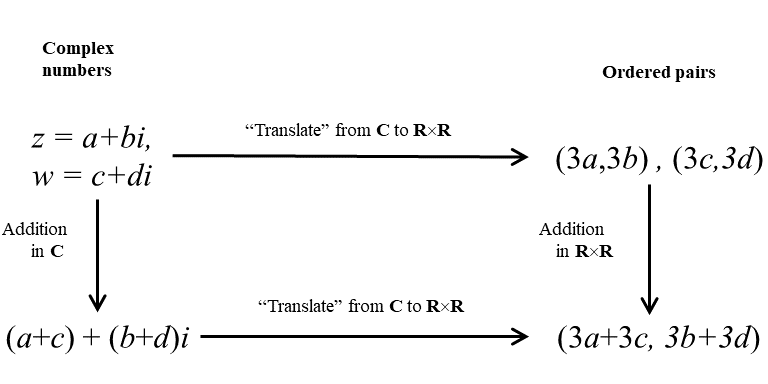
\includegraphics[width=4.in]
	         {images/CommDiagIso3.png}}
\end{figure}

\noindent\textbf{Exercise \ref{exercise:isomorph:iso_4}:}
%Prove that the function $h(a + bi) = (a+2, b+2)$ is {\bf not} an isomorphism from ${\mathbb C}$ to  ${\mathbb R} \times {\mathbb R}$.
%\hyperref[sec:isomorph:hints]{(*Hint*)}
%\\
\begin{figure}[H]
	   \center{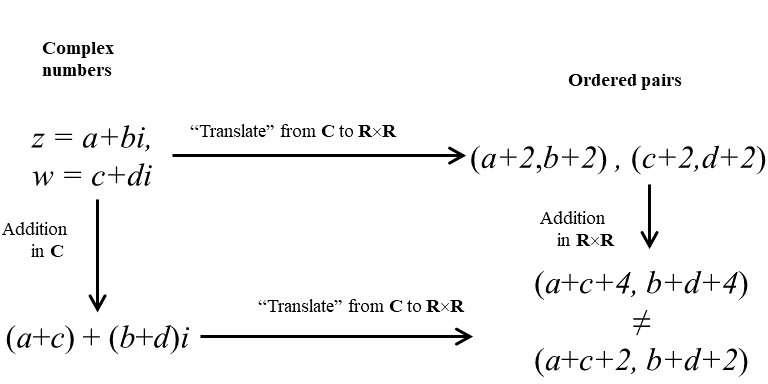
\includegraphics[width=4.in]
	         {images/CommDiagIso4.png}}
\end{figure}
Counterexample: Let $z = 3 + 4i, w = 2 + i \in {\mathbb C}$
\begin{align*}
\text{Then\ } z + w &= (3 + 4i) + (2 + i) &\text{(by substitution)}
\\
&= (3 + 2) + (4 + 1)i &\text{(complex addition)}
\\
&= 5 + 5i &\text{(basic algebra)}
\\
h(z + w) &= h(5 + 5i) &\text{(function of h)}
\\
&= (5 + 2, 5 + 2) &\text{(def of h)}
\\
&= (7, 7) &\text{(algebra)}
\\
h(z) + h(w) &= h(3 + 4i) + h(2 + i) &\text{(by substitution)}
\\
&= (3 + 2, 4 + 2) + (2 + 2, 1 + 2) &\text{(by def of h)}
\\
&= (5, 6) + (4, 3) &\text{(by algebra)}
\\
&= (5 + 4, 6 + 3) &\text{(by addition)}
\\
&= (9, 9) &\text{(algebra)}
\end{align*}
but $h(z + w) = (7, 7) \neq (9, 9) = h(z) + h(w)$
\\
so $h$ is not an isomorphism
\\
\\

\noindent\textbf{Exercise \ref{exercise:isomorph:iso_7}:}
%Determine whether each of the following functions are isomorphisms between the groups in Example~\ref{example:isomorph:sym_ex}. Justify your answers. 
\begin{enumerate}[(a)]
\item
%$ f: {\mathbb Z_4}  \longrightarrow \langle i \rangle$ defined by 
%\[  
%f(0) = 1,~~
% f(1) = -1,~~
% f(2) = i,~~
% f(3) = -i.
%\]
To show that $f$ is not an isomorphism, it is sufficient to find one example where the isomorphism relation fails.
We have:  $f(1+1) = f(2) = i$  but $f(1) \cdot f(1) = (-1)(-1) = 1$.  It follows that $f(1+1) \neq f(1)\cdot f(1)$, so $f$ is not an isomorphism.

\item
%$ g: {\mathbb Z_4}  \longrightarrow R_4$ defined by 
%\[ 
%g(0) = \var{id},~~
%g(1) = r_{270},~~
%g(2) = r_{90} ,~~
%g(3) = r_{180}. 
%\]
Verify that $g(1+1) \neq g(1)\cdot g(1)$, which shows that $g$ is not an isomorphsim.\\

\item
The Cayley table for $\langle i \rangle$ is:

\begin{multicols}{2}
\begin{table}[H]
{\small
\begin{center}
\begin{tabular}{c|cccccccc}
$\cdot$ & 1 & i & -1 & -i  \\
\hline
1        & 1 & i & -1 & -i  \\
i       & i & -1 & -i & 1  \\
-1       & -1 & -i & 1 & i \\
-i    & -i & 1 & i & -1 \\
\end{tabular}
\end{center}
}
\end{table}
\end{multicols}
We replace the elements in the above table with their images under $h$ and obtain:

\begin{multicols}{2}
\begin{table}[H]
{\small
\begin{center}
\begin{tabular}{c|cccccccc}
$\compose$ & id &$r_{270}$ &$ r_{180}$ & $r_{90}$  \\
\hline
id        & id & $r_{270}$ &$r_{180}$ & $r_{90}$  \\
$r_{270}$ & $r_{270}$ &$r_{180}$ & $r_{90}$ & id \\
$r_{180}$ &$r_{180}$ & $r_{90}$ & id& $r_{270}$  \\
$r_{90}$   & $r_{90}$ & id& $r_{270}$ &$r_{180}$ \\
\end{tabular}
\end{center}
}
\end{table}
\end{multicols}
This agrees with the Cayley table for $R_4$ (with the rows and columns rearranged), so $h$ is an isomorphism.

\item
Not an isomorphism: find an example that doesn't work.

\end{enumerate}

\noindent\textbf{Exercise \ref{exercise:isomorph:iso_6}:}

\begin{enumerate}[(a)]
\item
$ 0 \rightarrow 1;\,\,1\rightarrow -i; \,\,2 \rightarrow -1;\,\, 3 \rightarrow i$

\item
$ 1 \rightarrow id;\,\,i \rightarrow -r_{270} \,\,-1 \rightarrow r_{180};\,\, -i \rightarrow r_{90}$

\item
$ 0 \rightarrow id;\,\,1 \rightarrow -r_{270} \,\,2 \rightarrow r_{180};\,\, 3 \rightarrow r_{90}$
\end{enumerate}

\noindent\textbf{Exercise \ref{exercise:isomorph:iso_8}:}
\begin{enumerate}[(a)]
\item
For the solution to (a), take the solution to (b) and replace $a$ with 5.
\item
%Let $a$ be a nonzero real number, and consider the function $\phi_a : \mathbb{R} \rightarrow \mathbb{R}$ defined by:  $\phi_a(x) = ax$.  Show that $\phi_a$ defines an isomorphism. What are the two isomorphic groups involved?
%\\
%\\
First, note that $\phi$ is a bijection since it is invertible:  $\phi_a^{-1}(y) = y/a$.
Next, let $x,y \in {\mathbb R}$ (note the group operation is addition, since $ 0 \in {\mathbb R}$).
\begin{align*}
\phi_a(x \circ y) &= \phi_a(x + y) &\text{(by group operations)}
\\
&= a(x + y) &\text{(by definition\ } \phi_a)
\\
&= ax + ay &\text{(by distributive property)}
\\
\text{also,\ } \phi_a(x) \circ \phi_a(y) &= \phi_a(x) + \phi_a(y) &\text{(by group operations)}
\\
&= a(x) + a(y) &\text{(by definition\ } \phi_a)
\\
&= ax + ay &\text{(by basic algebra)}
\end{align*}
Since $\phi_a(x \circ y) = \phi_a(x) \circ \phi_a(y)$, we have concluded that $\phi_a$ is an isomorphism.
\\
The result shows that ${\mathbb R}$ is isomorphic to itself.
\\
\end{enumerate}

\noindent\textbf{Exercise \ref{exercise:isomorph:phi_id}:}
%Fill in the blanks in the following proof of Proposition~\ref{IsoId}:
%\medskip

%\noindent
%Given that $e$ is the identity of \underline{$~<1>~$} and $h$ is an arbitrary element of \underline{$~<2>~$}.  Since $\phi$ is a bijection, then there exists $g \in \underline{~<3>~}$ such that $\phi(\underline{~<4>~}) = h$.  Then  we have:
%\begin{align*}
%\phi(e) \circ h &= \phi(e) \circ \phi(\underline{~<5>~}) & \textrm{(substitution)}\\
%&= \phi( e \cdot \underline{~<6>~}) & \textrm{(definition of~} \underline{~<7>~})\\
%&= \phi( \underline{~<8>~}) & \textrm{(definition of \underline{~<9>~})}\\
%&= h & \textrm{(substitution)}
%\end{align*}
%Following the same steps, we can also show
%\begin{align*}
%h \circ \phi(e) = \underline{~<10>~}.
%\end{align*}
%It follows from the definition of identity that $\underline{~<11>~}$ is the identity of the group $\underline{~<12>~}$.

\begin{multicols}{3}
\begin{enumerate}
\item
$G$

\item
$H$

\item
$G$

\item
$g$

\item
$g$

\item
$g$

\item
isomorphism

\item
$g$

\item
identity

\item
$h$

\item
$\phi(e)$

\item
$H$
\end{enumerate}
\end{multicols}

\noindent\textbf{Exercise \ref{exercise:isomorph:phi_inverse}:}
%Fill in the blanks in the following proof of Proposition~\ref{IsoInv}:
%\medskip
%
%\noindent
%Let $e$ and $f$ be the identities of $G$ and $H$, respectively. Given that $g \in \underline{~<1>~}$, we have:
%\begin{align*}
%\phi(g) \circ \phi(g^{-1}) &= \phi(g \cdot g^{-1}) & \textrm{(definition of}~\underline{~<2>~})\\
%&= \phi(e) &\textrm{(definition of}~\underline{~<3>~})\\
%&= f &\textrm{(Proposition}~\underline{~<4>~} ).
%\end{align*}
%Using the same steps, we can also show
%\begin{align*}
%\phi(g^{-1}) \circ \phi(g) = \underline{~<5>~}.
%\end{align*}
%By the definition of inverse, it follows that
%\begin{align*}
%( \phi(g))^{-1} = \underline{~<6>~}.
%\end{align*}

\begin{multicols}{3}
\begin{enumerate}
\item
$G$

\item
isomorphism

\item
inverse

\item
Proposition~\ref{proposition:isomorph:IsoId}

\item
$f$

\item
$\phi(g^{-1})$
\end{enumerate}
\end{multicols}

\noindent\textbf{Exercise \ref{exercise:isomorph:InvCompIso}:}
\\
\begin{enumerate}[(a)]
\item
%Given that  $\phi : G \rightarrow H$ is an  isomorphism, show that  $\phi^{-1} : H \rightarrow G$ is also an  isomorphism.
%\hyperref[sec:isomorph:hints]{(*Hint*)}
%\\
%\\
Proof:  First, it is clear that $\phi^{-1}$ is invertible, and hence a bijection.
\\
Given $x, y \in H$ then, let $a = \phi^{-1}(x), b = \phi^{-1}(y)$
\begin{align*}
\implies \phi(a) &= x &\text{(definition of inverse)}
\\
\phi(b) &= y &\text{(definition of inverse)}
\\
\phi(a \cdot b) &= \phi(a) \circ \phi(b) &\text{(by Definition~\ref{isomorph_defn})}
\\
\phi(\phi^{-1}(x) \cdot \phi^{-1}(y)) &= x \circ y &\text{(substitution)}
\\
\phi^{-1}(\phi(\phi^{-1}(x) \cdot \phi^{-1}(y))) &= \phi^{-1}(x \circ y) &\text{(left multiply by\ } \phi^{-1})
\\
\phi^{-1}(x) \cdot \phi^{-1}(y) &= \phi^{-1}(x \circ y) &\text{(def of inverse)}
\end{align*}
Therefore $\phi^{-1}$ is an isomorphism by Definition~\ref{isomorph_defn}.
\\

\item
%Given that  $\phi : G \rightarrow H$ and $\psi : H \rightarrow K$ are  isomorphisms, show that  $\psi \circ\phi:G \rightarrow K$ is also an  isomorphism.
%\hyperref[sec:isomorph:hints]{(*Hint*)}
%\\
%\\
Show: $(i)$ Show that $\psi \circ \phi$ is a bijection and $(ii)\ \psi \circ \phi$ preserves group operation i.e. $\psi \circ \phi(a \cdot b) = (\psi \circ \phi(a)) \times (\psi \circ \phi(b))$.
	\begin{enumerate}[($i$)]
	\item
	\begin{align*}
	\psi \ \circ \ \phi(a \cdot b) &= \psi(\phi(a \cdot b)) &\text{(by definition of composition)}
	\\
	&=\psi(\phi(a) \cdot \phi(b)) &(\phi \text{\ is a bijection, operation of\ } H \text{\ is\ } \cdot)
	\\
	&= \psi(\phi(a)) \times \psi(\phi(b)) &(\psi \text{\ is a bijection, operation of\ } K \text{\ is\ } \times)
	\\
	&= (\psi \circ \phi(a)) \times (\psi \circ \phi(b)) &\text{(group operation is preserved)}
	\end{align*}

	\item
	$\psi \circ \phi(a \cdot b) = \psi \circ \phi$ \quad (by definition of composition)
	\end{enumerate}
and by Exercise \ref{exercise:Functions:BijectionComposeExer}, if $\psi$ and $\phi$ are bijections, then $\psi \circ \phi$ is a bijection.
\end{enumerate}

\noindent\textbf{Exercise \ref{exercise:isomorph:GpEquivRel}:}
%\\
%Prove Proposition~\ref{GpEquivRel}.
%\hyperref[sec:isomorph:hints]{(*Hint*)}
%\\
\\
Proof: Show that it is $(i)$ reflexive: $G \cong G$ , $(ii)$ symmetric: $G \cong H \implies H \cong G$, and $(iii)$ transitive: $G \cong H$ and $H \cong K \implies G \cong K$. 
\begin{enumerate}[($i$)]
\item
Define $\phi: G \rightarrow G$ by $\phi(x) = x$.  $\phi$ is a bijection that satisfies the isomorphism property.  So $G$ is isomorphic to iself.

\item
Given $G \cong H$, then $\exists \phi: G\rightarrow H$, such that $\phi$ is an isomorphism. Then from Exercise \ref{exercise:isomorph:InvCompIso}a, $\phi^{-1}$ is also an isomorphism and so $H \cong G$. This shows that $G \cong H \implies H \cong G$, so $\cong$ is symmetric.

\item
Let $G \cong H$ and $H \cong K$. Which we can define as: $\phi: G \rightarrow H$ and $\psi: H \rightarrow K$, then using Exercise \ref{exercise:isomorph:InvCompIso}b we know that $\phi \circ \psi$ is also an isomorphism and therefore $\cong$ is transitive.
\end{enumerate}

\noindent\textbf{Exercise \ref{exercise:isomorph:e_isomorph_proof}:}
%Define the function $\psi$ by: $\psi(x) = e^x$ for $x \in \mathbb{R}$.
\begin{enumerate}[(a)]
\item
%Given that the domain of $\psi$ is all real numbers, what is the range of $\psi$?
%\\
%\\
Domain: ${\mathbb R}$.  Range: ${\mathbb R}^+$.

\item
%Prove that $\psi(x)$ is a bijection between its domain and range.
%\\
%\\
From calculus we know that the natural logarithm function $\log: {\mathbb R}^+ \rightarrow {\mathbb R}$ is the inverse of the exponetial function.  Since $\psi$ has an inverse, it is a bijection.  

\item
%Find group operations on the domain and range of $\psi$ such that $\psi(x)$ preserves operations; i.e. $\psi(x \cdot y) = \psi(x)\compose \psi(y)$, where $\cdot$  and $\compose$ are the group operations on the domain and range,respectively. Verify that $\psi$ does indeed preserve operations for these two operations.
%\\
%\\
Let $x, y \in {\mathbb R}$ and $\psi: {\mathbb R} \rightarrow {\mathbb R}^+$ where $\psi(a) = e^a$, then
\begin{align*}
\psi(x + y) &= e^{(x + y)} &\text{(by definition of\ } \psi)
\\
&= (e^x)(e^y) &\text{(by rules of exponents)}
\\
&= \psi(x) \cdot \psi(y) &\text{(definition of\ } \psi)
\end{align*}

\item
%Now that we know $\psi(x)$ is an isomorphism, what can we conclude about $({\mathbb R}^+,\cdot)$ and $({\mathbb R},+)$?
%\\
%\\
%\\
Since we have shown that $\psi$ is a bijection between $({\mathbb R},+)$ and $({\mathbb R}^+,\cdot)$, then by Proposition \ref{proposition:isomorph:GpEquivRel} and Exercise \ref{exercise:isomorph:GpEquivRel}, we know that $({\mathbb R},+) \cong ({\mathbb R}^+,\cdot)$
\\
\end{enumerate}

\noindent\textbf{Exercise \ref{exercise:isomorph:ln_isomorph_proof}:}
\begin{enumerate}[(a)]
\item
%What is the largest possible domain and range of the natural logarithm function $\ln(x)$? (Consider only real logarithms,and not complex-valued logarithms or logarithms of complex numbers.)
%\\
Domain: ${\mathbb R}^+$  Range: ${\mathbb R}$

\item
%Using the previous exercise, the relation between natural logarithm and exponential function, as well as a result from earlier in this chapter, show that the natural logarithm function is an isomorphism. What are the two isomorphic groups?
%\\
Proof: Show that $\phi$ is a bijection we must show that it is $(i)$ 1:1 and $(ii)$ onto.
	\begin{enumerate}[($i$)]
	\item
	Let $x, y \in {\mathbb R}^+$, such that $\phi(x) = \phi(y)$, then
	\begin{align*}
	\ln(x) &= \ln(y) &\text{(by definition of\ } \phi)
	\\
	x &= y &\text{(take the e of both sides)}
	\end{align*}
	so $\phi$ is 1:1.

	\item
	Let $x = e^y$, for all $y \in {\mathbb R}$, then
	\begin{align*}
	\phi(x) &= \ln(x) &\text{(definition of\ } \phi)
	\\
	&= \ln(e^y) &\text{(by substitution)}
	\\
	&= y &\text{(by algebra)}
	\end{align*}
	so $\phi$ is onto.
	\end{enumerate}

	Since, $\phi$ is both 1:1 and onto, it is a bijection. 
	\\
	Now, we must show that group operations are preseved.
	\\
	Let $x, y \in {\mathbb R}^+$ and $\phi: {\mathbb R}^+ \rightarrow {\mathbb R}$, where $\phi(a) = \ln(a)$, then
	\\
	\begin{align*}
	\phi(x \cdot y) &= \ln(x \cdot y) &\text{(by definition of\ } \phi)
	\\
	&= \ln(x) + \ln(y) &\text{(by log rules)}
	\\
	&= \phi(x) + \phi(y) &\text{(by definition of\ } \phi \text{\ and group operations)}
	\end{align*}
	Since $\phi$ is a bijection and group operations are preserved $\phi$ is an isomorphism and the two groups are $({\mathbb R}^+, \cdot) \cong ({\mathbb R}, +)$.
	
\skipitems{2}
\end{enumerate}

\noindent\textbf{Exercise \ref{exercise:isomorph:iso_prac1}:}
\\
%%Prove that ${\mathbb Z} \cong n{\mathbb Z}$,  for every nonzero integer $n$.
%\\
Proof:  We must show that $(i)$ a bijection exists and $(ii)$ group operations are preserved.
\\
Define $\phi: {\mathbb Z} \rightarrow n{\mathbb Z}$ such that $\phi(x) = nx \forall x \in {\mathbb Z}$ and $n \in {\mathbb Z}^*$
\begin{enumerate}[($i$)]
\item
$\phi$ has an inverse function:  $\phi^{-1}(x) = x/n \forall x \in n{\mathbb Z}$.  Since $\phi$ is invertible, it is a bijection.

\item
Let $x, y \in {\mathbb Z}$ and define $\phi: {\mathbb Z} \rightarrow n{\mathbb Z}$ such that $\phi(a) = n\cdot a$, then
\\
\begin{align*}
\phi(x + y) &= n(x + y) &\text{(by substitution)}
\\
&= n\cdot x + n\cdot y &\text{(by distribution)}
\\
&= \phi(x) + \phi(y) &\text{(by definition of\ } \phi)
\end{align*}
This shows that the group operation is preserved.  
\end{enumerate}
Since $\phi$  is a bijection from ${\mathbb Z} \rightarrow n{\mathbb Z}$ that preserves group operations, then by definition, ${\mathbb Z} \cong n{\mathbb Z}$.
\\
\\

\noindent\textbf{Exercise \ref{exercise:isomorph:U8_U12_Cayley}:}
%Give the Cayley tables for $U(8)$ and $U(12)$.
\begin{multicols}{2}

\begin{table}[H]
\caption{Cayley table for $U(8)$}
{\small
\begin{center}
\begin{tabular}{c|cccccccc}
$\cdot$ & 1 & 3 & 5 & 7  \\
\hline
1        & 1 & 3 & 5 & 7  \\
3       & 3 & 1 & 7 & 5  \\
5       & 5 & 7 & 1 & 3 \\
7       & 7 & 5 & 3 & 1 \\
\end{tabular}
\end{center}
}
\end{table}

\begin{table}[H]
\caption{Cayley table for $U(12)$}
{\small
\begin{center}
\begin{tabular}{c|cccccccc}
$\cdot$ & 1 & 5 & 7 & 11  \\
\hline
1        & 1 & 5 & 7 & 11  \\
5       & 5 & 1 & 11 & 7 \\
7       & 7 & 11 & 1 & 5  \\
11      & 11 & 7 & 5 & 1 \\
\end{tabular}
\end{center}
}
\end{table}
\end{multicols}
\noindent $U(8)  \rightarrow U(12)$ is an isomorphism.  $\phi$ is 1:1 and onto, and it preserves the group operations so $U(8) \cong U(12)$ as per the book. 
\\
\\

\noindent\textbf{Exercise \ref{exercise:isomorph:U8_U12_other}:}
\begin{enumerate}[(a)]
\skipitems{1}

\item
Define a different isomorphism between $U(8)$ and $U(12)$, and use Cayley tables to verify that it's an isomorphism. 
\begin{multicols}{2}
\begin{table}[H]
\caption{Cayley table for $U(8)$}
{\small
\begin{center}
\begin{tabular}{c|cccccccc}
$\cdot$ & 1 & 3 & 5 & 7  \\
\hline
1        & 1 & 3 & 5 & 7  \\
3       & 3 & 1 & 7 & 5  \\
5       & 5 & 7 & 1 & 3 \\
7       & 7 & 5 & 3 & 1 \\
\end{tabular}
\end{center}
}
\end{table}

\begin{table}[H]
\caption{Cayley table for $U(12)$}
{\small
\begin{center}
\begin{tabular}{c|cccccccc}
$\cdot$ & 1 & 7 & 5 & 11  \\
\hline
1        & 1 & 7 & 5 & 11  \\
7       & 7 & 1 & 11 & 5 \\
5       & 5 & 11 & 1 & 7  \\
11      & 11 & 5 & 7 & 1 \\
\end{tabular}
\end{center}
}
\end{table}
\end{multicols}
$\psi : U(8) \rightarrow U(12)$, given by: $1\mapsto 1, 3 \mapsto 7, 5 \mapsto 5$, and $7 \mapsto 11$, so $\psi$ is also an isomorphism.
\end{enumerate}

\noindent\textbf{Exercise \ref{exercise:isomorph:U8_U12_Z2Z2}:}
%Prove that both $U(8)$ and $U(12)$ are isomorphic to ${\mathbb Z}_2 \times {\mathbb Z}_2$ (recall $\mathbb{Z}_2 \times \mathbb{Z}_2$ is the set of all pairs $(a,b)$ with $a,b \in \mathbb{Z}_2$, where 
%the group operation is addition mod 2 on each element in the pair). 
\begin{multicols}{3}
\begin{table}[H]
\caption{Cayley table for $U(8)$}
{\small
\begin{center}
\begin{tabular}{c|cccccccc}
$\cdot$ & 1 & 3 & 5 & 7  \\
\hline
1        & 1 & 3 & 5 & 7  \\
3       & 3 & 1 & 7 & 5  \\
5       & 5 & 7 & 1 & 3 \\
7       & 7 & 5 & 3 & 1 \\
\end{tabular}
\end{center}
}
\end{table}

\begin{table}[H]
\caption{Cayley table for $U(12)$}
{\small
\begin{center}
\begin{tabular}{c|cccccccc}
$\cdot$ & 1 & 5 & 7 & 11  \\
\hline
1        & 1 & 5 & 7 & 11  \\
5       & 5 & 1 & 11 & 7 \\
7       & 7 & 11 & 1 & 5  \\
11      & 11 & 7 & 5 & 1 \\
\end{tabular}
\end{center}
}
\end{table}

\begin{table}[H]
\caption{Cayley table for ${\mathbb Z}_2 \times {\mathbb Z}_2$}
{\small
\begin{center}
\begin{tabular}{c|cccccccc}
$+$ & (0, 0) & (1, 0) & (0, 1) & (1, 1)  \\
\hline
(0, 0)        & (0, 0) & (1, 0) & (0, 1) & (1, 1)  \\
(1, 0)       & (1, 0) & (0, 0) & (1, 1) & (0, 1)  \\
(0, 1)       & (0, 1) & (1, 1) & (0, 0) & (1, 0) \\
(1, 1)       & (1, 1) & (0, 1) & (1, 0) & (0, 0) \\
\end{tabular}
\end{center}
}
\end{table}
\end{multicols}
\noindent If we define $\phi : U(8) \rightarrow {\mathbb Z}_2 \times {\mathbb Z}_2$, given by: $1\mapsto (0, 0), 3 \mapsto (1, 0), 5 \mapsto (0, 1)$, and $7 \mapsto (1, 1)$, then we can see the function is 1:1, and onto, and also the group operation is preserved. 
\\
\\
We can define $\psi: U(12) \rightarrow {\mathbb Z}_2 \times {\mathbb Z}_2$, given by $1\mapsto (0, 0), 5 \mapsto (1, 0), 7 \mapsto (0, 1)$, and $11 \mapsto (1, 1)$, then we can see the function is 1:1, and onto, and also the group operation is preserved. 
\\
\\

\noindent\textbf{Exercise \ref{exercise:isomorph:iso_prac3}:}
%Prove that $U(8)$ is isomorphic to the group of matrices
%\[
%\begin{pmatrix}
%1 & 0 \\
%0 & 1
%\end{pmatrix},
%\begin{pmatrix}
%1 & 0 \\
%0 & -1
%\end{pmatrix},
%\begin{pmatrix}
%-1 & 0 \\
%0 & 1
%\end{pmatrix},
%\begin{pmatrix}
%-1 & 0 \\
%0 & -1
%\end{pmatrix}.
%\]
%\\
\begin{table}[H]
\caption{Cayley table for $U(8)$}
{\small
\begin{center}
\begin{tabular}{c|cccccccc}
$\cdot$ & 1 & 3 & 5 & 7  \\
\hline
1        & 1 & 3 & 5 & 7  \\
3       & 3 & 1 & 7 & 5  \\
5       & 5 & 7 & 1 & 3 \\
7       & 7 & 5 & 3 & 1 \\
\end{tabular}
\end{center}
}
\end{table}


\begin{table}[H]
\caption{Cayley table for$A$ ( group of 4 matrices)}
{\small
\begin{center}
\begin{tabular}{c|cccccccc}
$\cdot$ & $\begin{pmatrix}1 & 0 \\ 0 & 1 \end{pmatrix}$ 
& $\begin{pmatrix}1 & 0 \\0 & -1\end{pmatrix}$ 
& $\begin{pmatrix}-1 & 0 \\0 & 1\end{pmatrix}$ 
& $\begin{pmatrix}-1 & 0 \\0 & -1\end{pmatrix}$  \\
\hline
$\begin{pmatrix}1 & 0 \\ 0 & 1 \end{pmatrix}$ 
& $\begin{pmatrix}1 & 0 \\ 0 & 1 \end{pmatrix}$ 
& $\begin{pmatrix}1 & 0 \\0 & -1\end{pmatrix}$ 
& $\begin{pmatrix}-1 & 0 \\0 & 1\end{pmatrix}$
& $\begin{pmatrix}-1 & 0 \\0 & -1\end{pmatrix}$\\
\\
$\begin{pmatrix}1 & 0 \\0 & -1\end{pmatrix}$       
& $\begin{pmatrix}1 & 0 \\0 & -1\end{pmatrix}$ 
& $\begin{pmatrix}1 & 0 \\ 0 & 1 \end{pmatrix}$ 
& $\begin{pmatrix}-1 & 0 \\0 & -1\end{pmatrix}$ 
& $\begin{pmatrix}-1 & 0 \\0 & 1\end{pmatrix}$ \\
\\
$\begin{pmatrix}-1 & 0 \\0 & 1\end{pmatrix}$       
& $\begin{pmatrix}-1 & 0 \\0 & 1\end{pmatrix}$ 
& $\begin{pmatrix}-1 & 0 \\0 & -1\end{pmatrix}$ 
& $\begin{pmatrix}1 & 0 \\ 0 & 1 \end{pmatrix}$ 
& $\begin{pmatrix}1 & 0 \\0 & -1\end{pmatrix}$ \\
\\
$\begin{pmatrix}-1 & 0 \\0 & -1\end{pmatrix}$       
& $\begin{pmatrix}-1 & 0 \\0 & -1\end{pmatrix}$ 
& $\begin{pmatrix}-1 & 0 \\0 & 1\end{pmatrix}$ 
& $\begin{pmatrix}1 & 0 \\0 & -1\end{pmatrix}$ 
& $\begin{pmatrix}1 & 0 \\ 0 & 1 \end{pmatrix}$ \\
\end{tabular}
\end{center}
}
\end{table}

\noindent We can define $\phi: U(8) \rightarrow A$, where $A$ is the group of 4 matrices, given by  $1\mapsto \begin{pmatrix}1 & 0 \\ 0 & 1 \end{pmatrix}, 3 \mapsto \begin{pmatrix}1 & 0 \\0 & -1\end{pmatrix},
\\
5 \mapsto \begin{pmatrix}-1 & 0 \\0 & 1\end{pmatrix}$, and $7 \mapsto \begin{pmatrix}-1 & 0 \\0 & -1\end{pmatrix}$, then we can see the function is 1:1, onto, and also the group operation is preserved. 
\\
\\

\noindent\textbf{Exercise \ref{exercise:isomorph:iso_prac4}:}
%Show that the matrices
%\begin{gather*}
%\Big\{
%\begin{pmatrix}
%1 & 0 & 0 \\
%0 & 1 & 0 \\
%0 & 0 & 1
%\end{pmatrix},
%\begin{pmatrix}
%1 & 0 & 0 \\
%0 & 0 & 1 \\
%0 & 1 & 0
%\end{pmatrix},
%\begin{pmatrix}
%0 & 1 & 0 \\
%1 & 0 & 0 \\
%0 & 0 & 1
%\end{pmatrix}, \\
%\begin{pmatrix}
%0 & 0 & 1 \\
%1 & 0 & 0 \\
%0 & 1 & 0
%\end{pmatrix},
%\begin{pmatrix}
%0 & 0 & 1 \\
%0 & 1 & 0 \\
%1 & 0 & 0
%\end{pmatrix},
%\begin{pmatrix}
%0 & 1 & 0 \\
%0 & 0 & 1 \\
%1 & 0 & 0
%\end{pmatrix}
%\Big\}
%\end{gather*}
%form a group. Find an isomorphism of $G$ with a more familiar group of
%order~6.
%\\
\begin{multicols}{3}
$A =
\begin{pmatrix}
1 & 0 & 0 \\
0 & 1 & 0 \\
0 & 0 & 1
\end{pmatrix}$

$B =
\begin{pmatrix}
1 & 0 & 0 \\
0 & 0 & 1 \\
0 & 1 & 0
\end{pmatrix}$

$C =
\begin{pmatrix}
0 & 1 & 0 \\
1 & 0 & 0 \\
0 & 0 & 1
\end{pmatrix}$

$D =
\begin{pmatrix}
0 & 0 & 1 \\
1 & 0 & 0 \\
0 & 1 & 0
\end{pmatrix}$

$E =
\begin{pmatrix}
0 & 0 & 1 \\
0 & 1 & 0 \\
1 & 0 & 0
\end{pmatrix}$

$F =
\begin{pmatrix}
0 & 1 & 0 \\
0 & 0 & 1 \\
1 & 0 & 0
\end{pmatrix}$
\end{multicols}

\begin{table}[H]
\caption{Cayley table for$A$ - group of 4 matrices}
{\small
\begin{center}
\begin{tabular}{c|cccccc}
$\cdot$ & $A$
& $B$ 
& $C$
& $D$
& $E$  
& $F$
\\
\\
\hline
$A$
&$A$
& $B$ 
& $C$
& $D$
& $E$  
& $F$\\
\\
$B$    
& $B$ 
& $A$
& $F$
& $E$
& $D$
& $C$\\
\\
$C$  
& $C$
&  $D$
&$A$
& $B$ 
& $F$
& $E$\\
\\
 $D$ 
&  $D$
& $C$
& $E$
&$F$
& $B$
& $A$\\
\\
$E$
& $E$
& $F$
&  $D$
& $C$
& $A$
& $B$
\\
\\
$F$
& $F$
& $E$
& $B$
& $A$
& $C$
& $D$
\\
\\
\end{tabular}
\end{center}
}
\end{table}

\noindent
The Cayley table shows closure, there is an identity element $I_3$, every element has an inverse such that $x \circ x^{-1} = \var{id}$, and you can see associative from the table. Therefore, $G$ is a group.  
\\
If you use Remark~\ref{remark:symmetries:comp_order} and the Cayley table created in Exercise \ref{exercise:permute:11}a, you will see that $A \mapsto \var{id}, B \mapsto \mu_1, C \mapsto \mu_3, D \mapsto \rho_1, E \mapsto \mu_2$, and $F \mapsto \rho_2$, then we can see the function is 1:1, onto, and also the group operation is preserved. 
\\
\\

\noindent\textbf{Exercise \ref{exercise:isomorph:factor_S3}:}
%Prove that the factor group $S_3/A_3 \cong {\mathbb Z}_2$.
\begin{multicols}{2}
\begin{table}[H]
\caption{Cayley table for $S_3/A_3$}
{\small
\begin{center}
\begin{tabular}{c|ccc}
$\circ$ &$ A_3$ & $(12)A_3$  \\
\hline
$A_3$        &$A_3$ &$ (12)A_3$  \\
$(12)A_3$  & $(12)A_3$  &$A_3$   \\
\end{tabular}
\end{center}
}
\end{table}

\begin{table}[H]
\caption{Cayley table for${\mathbb Z}_2$}
{\small
\begin{center}
\begin{tabular}{c|ccc}
$\oplus$ & 0 & 1 \\

\hline
0 & 0 & 1 \\ 
1& 1 & 0 \\
\end{tabular}
\end{center}
}
\end{table}
\end{multicols}
\noindent We can define $\phi:S_3/A_3 \rightarrow {\mathbb Z}_2$,  given by  $A_3\mapsto 0,  (12)A_3 \mapsto 1$, so $S_3/A_3 \cong {\mathbb Z}_2$.
\\
\\

\noindent\textbf{Exercise \ref{exercise:isomorph:factor_iso}:}
%Prove the following:
\begin{enumerate}[(a)]
\item
%${\mathbb Z}/ 3 {\mathbb Z} \cong {\mathbb Z}_3$
\begin{multicols}{2}
\begin{table}[H]
\caption{Cayley table for ${\mathbb Z}/ 3 {\mathbb Z}$}
{\small
\begin{center}
\begin{tabular}{c|ccc}
$\cdot$ & $ 3 {\mathbb Z}$ & $ 3 {\mathbb Z} + 1$ & $ 3 {\mathbb Z} + 2$ \\
\hline
$ 3 {\mathbb Z}$ & $ 3 {\mathbb Z}$ & $ 3 {\mathbb Z} + 1$ & $ 3 {\mathbb Z} + 2 $  \\
$ 3 {\mathbb Z} + 1$  & $ 3 {\mathbb Z} + 1$  & $ 3 {\mathbb Z} + 2$ &  $3 {\mathbb Z}$   \\
$ 3 {\mathbb Z} + 2$  & $ 3 {\mathbb Z} + 2$ & $ 3 {\mathbb Z}$ & $ 3 {\mathbb Z} + 1$ \\
\end{tabular}
\end{center}
}
\end{table}

\begin{table}[H]
\caption{Cayley table for${\mathbb Z}_3$}
{\small
\begin{center}
\begin{tabular}{c|ccc}
$\oplus$ & 0 & 1  & 2\\

\hline
0 & 0 & 1  & 2\\ 
1& 1 & 2 & 0\\
2 & 2 & 0 & 1\\
\end{tabular}
\end{center}
}
\end{table}
\end{multicols}
We can define $\phi:{\mathbb Z}/ 3 {\mathbb Z} \rightarrow {\mathbb Z}_3$,  given by  $3 {\mathbb Z} \mapsto 0,  3 {\mathbb Z} + 1 \mapsto 1$, and $3 {\mathbb Z} + 2 \mapsto 2$. Since it is a group and it retains group operations we've shown $S_3/A_3 \cong {\mathbb Z}_3$.

\skipitems{1}
\end{enumerate}

\noindent\textbf{Exercise \ref{exercise:isomorph:another_pattern}:}
%By using the preceding propositions and comparing diagonal elements of Cayley tables, prove  that ${\mathbb Z}_4 \ncong U(12)$.
\begin{itemize}
\item
Using the Cayley table for $U(12)$, you see that the identity element, 1, is the entry for each element composed with itself.
\begin{table}[H]
\caption{Cayley table for $U(12)$}
{\small
\begin{center}
\begin{tabular}{c|cccccccc}
$\cdot$ & 1 & 5 & 7 & 11  \\
\hline
1        & 1 & 5 & 7 & 11  \\
5       & 5 & 1 & 11 & 7 \\
7       & 7 & 11 & 1 & 5  \\
11      & 11 & 7 & 5 & 1 \\
\end{tabular}
\end{center}
}
\end{table}

\item
If you rearranged the rows and columns of this Cayley table the identity element, 1, is the entry for each element composed with itself, so the pattern remains the same.
\begin{table}[H]
\caption{Cayley table for $U(12)$}
{\small
\begin{center}
\begin{tabular}{c|cccccccc}
$\cdot$ & 1 & 7 & 5 & 11  \\
\hline
1        & 1 & 7 & 5 & 11  \\
7       & 7 & 1 & 11 & 5 \\
5      & 5 & 11 & 1 & 7  \\
11      & 11 & 5 & 7 & 1 \\
\end{tabular}
\end{center}
}
\end{table}

\item
Therefore, if you compare the diagonal entries of the two Cayley tables you will see that there is no arrangement of compositions where they will be a bijection to each other.
\end{itemize}

\noindent\textbf{Exercise \ref{exercise:isomorph:iso_prac5}:}
%Prove or disprove: $U(8) \cong {\mathbb Z}_4$.
\begin{multicols}{2}
\begin{table}[H]
\caption{Cayley table for $U(8)$}
{\small
\begin{center}
\begin{tabular}{c|cccccccc}
$\cdot$ & 1 & 3 & 5 & 7  \\
\hline
1        & 1 & 3 & 5 & 7  \\
3       & 3 & 1 & 7 & 5  \\
5       & 5 & 7 & 1 & 3 \\
7       & 7 & 5 & 3 & 1 \\
\end{tabular}
\end{center}
}
\end{table}

\begin{table}[H]
\caption{Cayley table for ${\mathbb Z}_4$}
{\small
\begin{center}
\begin{tabular}{c|cccccccc}
$\oplus$ & 0 & 1 & 2 & 3  \\
\hline
0        & 0 & 1 & 2 & 3  \\
1       & 1 & 2 & 3 & 0  \\
2       & 2 & 3 & 0 & 1 \\
3       & 3 & 0 & 1 & 2 \\
\end{tabular}
\end{center}
}
\end{table}

\end{multicols}
\noindent The diagonal entries of the two Cayley cannot be arranged to create a bijection, because ${\mathbb Z}_4$ has an alternating diagonal, therefore they cannot be isomorphic, which also means they are not $\cong$.
\\
\\

\noindent\textbf{Exercise \ref{exercise:isomorph:iso_prac6}:}
%Let $\sigma$ be the permutation $(12)$, and let $\tau$ be the permutation $(34)$.
%Let $G$ be the set $\{ \var{id}, \sigma, \tau, \sigma\tau \}$ together with the operation of composition.
\begin{enumerate}[(a)]
\item
%Give the Cayley table for the group $G$.
\begin{table}[H]
\caption{Cayley table for $G =\{id, \sigma, \tau, \sigma\tau\}$}
{\small
\begin{center}
\begin{tabular}{c|cccccccc}
$\circ $ & id & $\sigma$ & $\tau$ & $\sigma\tau$  \\
\hline
id        & id & $\sigma$ & $\tau$  & $\sigma\tau$  \\
$\sigma$       & $\sigma$ & id & $\sigma\tau$ & $\tau$  \\
$\tau$      & $\tau$ & $\sigma\tau$ & id & $\sigma$ \\
$\sigma\tau$      & $\sigma\tau$  & $\tau$ & $\sigma$ & id \\
\end{tabular}
\end{center}
}
\end{table}

\item
%Prove or disprove: $G \cong {\mathbb Z}_4$.
\begin{table}[H]
\caption{Cayley table for ${\mathbb Z}_4$}
{\small
\begin{center}
\begin{tabular}{c|cccccccc}
$\oplus$ & 0 & 1 & 2 & 3  \\
\hline
0        & 0 & 1 & 2 & 3  \\
1       & 1 & 2 & 3 & 0  \\
2       & 2 & 3 & 0 & 1 \\
3       & 3 & 0 & 1 & 2 \\
\end{tabular}
\end{center}
}
\end{table}
The diagonal entries of the two Cayley cannot be arranged to create a bijection, therefore they cannot be isomorphic, which also means they are not $\cong$.

\item
Prove or disprove: $G \cong U(12)$.
\begin{table}[H]
\caption{Cayley table for $U(12)$}
{\small
\begin{center}
\begin{tabular}{c|cccccccc}
$\cdot$ & 1 & 5 & 7 & 11  \\
\hline
1        & 1 & 5 & 7 & 11  \\
5       & 5 & 1 & 11 & 7 \\
7       & 7 & 11 & 1 & 5  \\
11      & 11 & 7 & 5 & 1 \\
\end{tabular}
\end{center}
}
\end{table}
\end{enumerate}
We can define $\phi:G \rightarrow U(12)$,  given by  $\var{id} \mapsto 1,  \sigma \mapsto 5, \tau \mapsto 7$, and $\sigma\tau \mapsto 11$. Since it is a group and it retains group operations we've shown $G \cong U(12)$.
\\
\\

\noindent\textbf{Exercise \ref{exercise:isomorph:cyclic_noncyclic}:}
%Prove Proposition \ref{proposition:isomorph:cyclic_noncyclic}.
\\
Proof: Suppose there exists an isomorphism $\phi: G \rightarrow H$ for a cyclic group $G = \langle a \rangle$ and a non-cyclic group $H$.
\\
Let $h \in H$ such that $h = \phi(g)$ for some $g \in G$, then
\begin{align*}
h &= \phi(g) &\text{(by supposition)}
\\
&= \phi \underbrace{(a \cdot a \cdot \dotsc \cdot a)}_{\substack{a^n = g \\ (n\  \text{times})}} &\text{(by definition of cyclic groups\ } G = \langle a \rangle \implies a^n = g)
\\
&= \underbrace{\phi(a) \cdot \phi(a) \cdot \dotsc \cdot  \phi(a)}_{n\ \text{times}} &\text{(by definition of isomorphism)}
\end{align*}
So, then $h \in \langle \phi(a) \rangle$, but we supposed that $H$ was not a cyclic group, so this is a contradiction.
\\
Then our supposition must be false, if $G$ is a cyclic group, $G \cong H$, then $H$ must also by a cyclic group.
\\
\\

\noindent\textbf{Exercise \ref{exercise:isomorph:noniso_cyclic}:}
\begin{enumerate}[(a)]
\item
%Prove that ${\mathbb Q}$ is not isomorphic to ${\mathbb Z}$.
%\\
Proof: Suppose ${\mathbb Q}$ is cyclic, then ${\mathbb Q} = \langle a \rangle$ for some $a \in {\mathbb Q}$.
\\
Then ${\mathbb Q} = \{ \dotsc , -2a, -a, 0, a, 2a, \dotsc\}$.
\\
Consider, $\frac{a}{2}$, since $\frac{a}{2} \in {\mathbb Q} \implies \frac{a}{2} = ka \implies \frac{a}{2} - ka = 0 \implies a(\frac{1}{2} - k) = 0$.
\\
By the zero divisor property of ${\mathbb Q}$ this $\implies a = 0$ or $(\frac{1}{2} - k) = 0$ or $a = 0$ and $(\frac{1}{2} - k) = 0$.
\\
Since $\langle 0 \rangle = \{0\}$, so $a \neq 0$.
\\
Also, $k \in {\mathbb Z}$, which means $\frac{1}{2} - k \neq 0$, and so then $a(\frac{1}{2} - k) \neq 0$.
\\
This contradicts the supposition and therefore ${\mathbb Q}$ is not cyclic.

\item
%Prove that  ${\mathbb Z}_3 \times {\mathbb Z}_3$ is not isomorphic to ${\mathbb Z}_9$.
%\\
We showed in Example~\ref{example:groups:construct_Z6} that ${\mathbb Z}_6$ is cyclic.  ${\mathbb Z}_3$ and ${\mathbb Z}_4$ are cyclic based on the same procedure.
\\
Proof: Consider ${\mathbb Z}_3 \times {\mathbb Z}_3 = \{(0, 0), (0, 1), (0, 2), (1, 0), (1, 1), (1, 2), (2, 0), (2, 1), (2,2)\}$.
\\
Suppose  ${\mathbb Z}_3 \times {\mathbb Z}_3$ is cyclic, then ${\mathbb Z}_3 \times {\mathbb Z}_3 = \langle a \rangle$ for some $a \in {\mathbb Z}_3 \times {\mathbb Z}_3$, by exhaustion:
\begin{align*}
\langle(0, 0)\rangle &= \{(0, 0)\}
\\
\langle(0, 1)\rangle &= \{(0, 1), (0, 2), (0, 0)\}
\\
\langle(0, 2)\rangle &= \{(0, 2), (0, 1), (0, 0)\}
\\
\langle(1, 0)\rangle &= \{(1, 0), (2, 0), (0, 0)\}
\\
\langle(1, 1)\rangle &= \{(1, 1), (2,2), (0, 0)\}
\\
\langle(1, 2)\rangle &= \{(1, 2), (2, 1), (0, 0)\}
\\
\langle(2, 0)\rangle &= \{(2, 0), (1, 0), (0, 0)\}
\\
\langle(2, 1)\rangle &= \{(2, 1), (1, 2), (0, 0)\}
\\
\langle(2, 2)\rangle &= \{(2, 2), (1, 1), (0, 0)\}
\end{align*}
and we can see $\forall\ a \in {\mathbb Z}_3 \times {\mathbb Z}_3, \langle a \rangle \neq {\mathbb Z}_3 \times {\mathbb Z}_3$, so by definition is it not cyclic.
\\
Then, by Proposition~\ref{proposition:isomorph:cyclic_noncyclic}, since ${\mathbb Z}_9$ is cyclic and ${\mathbb Z}_3 \times {\mathbb Z}_3$ is not cyclic, ${\mathbb Z}_9 \ncong {\mathbb Z}_3 \times {\mathbb Z}_3$.

\item
%Prove that  $D_4 \ncong {\mathbb Z}_{24} / \langle 8 \rangle$
%\\
Proof: Consider $D_4$, where $|D_4| = 2n = 2 \cdot 4 = 8$    (by definition of $D_4$), by exhaustion:
\begin{align*}
\langle \var{id} \rangle &= \{\var{id}\}
\\
\langle r \rangle &= \{r, r^2, r^3, \var{id}\}
\\
\langle r^2 \rangle &= \{r^2, \var{id}\}
\\
\langle r^3 \rangle &= \{r^3, r^2, r, \var{id}\}
\\
\langle s \rangle &= \{s, \var{id}\}
\\
\langle s \circ r \rangle &= \{ s \circ r, \var{id}\}
\\
\langle s \circ r^2 \rangle &= \{s \circ r^2, \var{id}\}
\\
\langle s \circ r^3 \rangle &= \{s \circ r^3, \var{id}\}
\end{align*}
for $a \in D_4$ since for $\langle a \rangle \neq D_4, D_4$ is not cyclic.
\\
Then consider 
\begin{align*}
{\mathbb Z}_{24} / \langle 8 \rangle &= \{ \langle 8 \rangle, \langle 8 \rangle + 1, \langle 8 \rangle + 2, \langle 8 \rangle + 3, \langle 8 \rangle + 4, \langle 8 \rangle + 5, \langle 8 \rangle + 6, \langle 8 \rangle + 7\}
\\
\langle \langle 8 \rangle + 1 \rangle &= \{ \langle 8 \rangle + 1, \langle 8 \rangle + 2, \langle 8 \rangle + 3, \langle 8 \rangle + 4, \langle 8 \rangle + 5, \langle 8 \rangle + 6, \langle 8 \rangle + 7\}
\end{align*}
So ${\mathbb Z}_{24} / \langle 8 \rangle$ is a cyclic group. By Proposition \ref{proposition:isomorph:abelian_non-abelian}, a cyclic group cannot be isomorphic to a noncyclic group so  $D_4 \ncong {\mathbb Z}_{24} / \langle 8 \rangle$.
\end{enumerate}

\noindent\textbf{Exercise \ref{exercise:isomorph:phigprime_subgroup_H}:}
%Fill in the blanks of the following proof of Step (I)  (that is, $\phi(G')$ is a subgroup of $H$):
%\medskip

%Let us suppose that $G'$ is a subgroup of $G$. We claim that $\phi(G')$ is actually a subgroup of \underline{$~<1>~$}.  To show this, by Proposition~\ref{proposition:groups:subgroup_prove_2} it's enough to show that if $h_1$ and $h_2$ are elements of  $\phi(G')$, then $h_1 h_2^{-1}$ is also an element of \underline{$~<2>~$}.
%
%Now given that  $h_1, h_2 \in \phi(G')$, by the definition of $\phi(G')$ it must be true that there exist $g_1, g_2 \in \underline{~<3>~}$ such that $\phi(g_1) = h_1, \phi(g_2) = h_2$. But then we have 
%\begin{align*}
%h_1 h_2^{-1} &= \phi(g_1) \phi(g_2)^{-1} &\text{(by substitution)}\\
%&= \phi(g_1) \phi(g_2^{-1}) &(\text{by Proposition~}\underline{~<4>~})\\
%&= \phi(g_1 g_2^{-1}) &(\text{by the definition of }\underline{~<5>~}).
%\end{align*}
%Since $g_1 g_2^{-1}$ is an element of $G'$, it follows that $h_1 h_2^{-1} \in \underline{~<6>~}$. This completes the proof of Step (I).

\begin{multicols}{3}
\begin{enumerate}
\item
$H$

\item
$\phi(G')$

\item
$G'$

\item
\ref {proposition:isomorph:IsoInv}

\item
isomorphism

\item
$\phi(G')$
\end{enumerate}
\end{multicols}

\noindent\textbf{Exercise \ref{exercise:isomorph:gprime_phigprime_iso}:}
%Complete the following proof of Step (II) (that is, $G'$ and $\phi(G')$ are isomorphic). 
%\medskip
%
%Consider the function $\phi$ restricted to the set $G'$: that is, $\phi: G' \rightarrow \phi(G')$.  To  prove this gives an isomorphism from $G'$ to $\phi(G')$, we need to show (i) $\phi: G' \rightarrow \phi(G')$ is a bijection; and (ii) $\phi: G' \rightarrow \phi(G')$ has the operation-preserving property.
%
%To show (i), we note that by the definition of $\phi(G')$, for every $h \in \phi(G')$ there exists a $g \in \underline{~<1>~}$ such that $\phi(\underline{~<2>~}) = h$. It follows that $\phi$ maps $G'$ onto $\underline{~<3>~}$.  Also, if $g_1, g_2 \in G'$ and $\phi(g_1) = \phi(g_2)$, then since $\phi$ is a one-to-one function on $G$ it follows that $g_1 = \underline{~<4>~}$. From this it follows that $\phi$ is also a one-to-one function on $\underline{~<5>~}$.  We conclude that $\underline{~<6>~}$ is a bijection.
%
%To show (ii), given $g_1, g_2 \in \underline{~<7>~}$ we have that $\phi(g_1 g_2) = \underline{~<8>~}$ since by assumption $\phi$ is an isomorphism from \underline{$~<9>~$} to \underline{$~<10>~$}. This implies that $\phi$ also has the operation-preserving  property when it's considered as a function from  \underline{$~<11>~$} to \underline{$~<12>~$}.  This completes the proof of Step (II).

\begin{multicols}{3}
\begin{enumerate}
\item
$G'$

\item
$g$

\item
$\phi(G')$

\item
$g_2$

\item
$G'$

\item
$\phi$

\item
$G'$

\item
$\phi(g_1) \circ \phi(g_2)$

\item
$G'$

\item
$\phi(G')$

\item
$G'$

\item
$\phi(G')$
\end{enumerate}
\end{multicols}





\section{Solutions for ``Group Actions''}
\noindent\textbf{\textit{ (Chapter \ref{actions}})}\bigskip

\noindent(\emph{NOTE that in the problems that ask to give rotations, the listings are not exhaustive: other answers are possible.})

\noindent\textbf{Exercise \ref{exercise:actions:Cube1}}
\begin{enumerate}[(a)]
\item
%Give rotations that take the bottom face ($z_-$) to each of the faces $x_-,x_+,y_-,y_+$.
	\begin{multicols}{4}
	\begin{itemize}
	\item
	$z_-\rightarrow x_-$: 
		\begin{itemize}
		\item
		$r_y$
		
		\item
		$r_y^{-3} $ 
		\end{itemize}
				
	\item
	$z_-\rightarrow x_+$: 
		\begin{itemize}
		\item
		$r_y\compose r_z^2$
		
		\item
		$r_y^{-1}$
		
		\item
		$r_y^3$
		\end{itemize}
				
	\item
	$z_-\rightarrow y_-$: 
		\begin{itemize}
		\item
		$r_x^3$
		
		\item
		$r_x^{-1}$
		\end{itemize}
				
	\item
	$z_-\rightarrow y_+$:
		\begin{itemize}
		\item
		$r_x$
		
		\item
		$r_x^{-3}$
		\end{itemize}
				
	\end{itemize}
	\end{multicols}
	
\item
%Give rotations that take the face $y_- $ to each of the faces $x_-,x_+,y_+,z_-,z_+$.
\begin{multicols}{3}
	\begin{itemize}
	\item
	$y_-\rightarrow x_-$: 
		\begin{itemize}
		\item
		$r_z^{3}$
		
		\item
		$r_x^{3}$
		\end{itemize}
				
	\item
	$y_-\rightarrow x_+$:
		\begin{itemize}
		\item
		$r_z$
		
		\item
		$r_z^{-3}$
		\end{itemize}
				
	\item
	$y_-\rightarrow y_+$:   
		\begin{itemize}
		\item
		$r_z^{-2}$ 
		
		\item
		$r_z^{2}$
		\end{itemize}
	
	\columnbreak
	
	\item
	$y_-\rightarrow z_-$:    
		\begin{itemize}
		\item
		$r_x$
		
		\item
		$r_x^{-3}$
		\end{itemize}
		
	\item
	 $y_-\rightarrow z_+$
		\begin{itemize}
		\item
		$r_x^{-1}$
		
		\item
		$r_x^{3}$
		\end{itemize}
	\end{itemize}
	\end{multicols}
	
\item
%Let's define a notation for the cube's vertices as follows.  For example, $+++$ represents the vertex in the first octant ($x>0,y>0,z>0$).  The vertex $+-\,-$ will be in the octant where $x>0,y<0,z<0$ (Which is the vertex at lower left in Figure~\ref{fig:CubeRot}).  Give rotations that take the vertex $+-\,-$ to each of the of the vertices 
%\[ +++, ~-\,++,~+\,-\,+,~ ++\,-,~-\,-\,+,~-\,+\,-,~-\,-\,-. \]
\begin{multicols}{3}
	\begin{itemize}
	\item
	$+-\,-\rightarrow +++$: 
		\begin{itemize}
		\item
		$r_x^2$
		
		\item
		$r_x^{-2}$
		\end{itemize}
 
 	\item
 	$+-\,-\rightarrow -\,++$: 
 		\begin{itemize}
 		\item
 		$r_z \circ r_x^{2}$
 		\end{itemize}
 		
 	\item
 	$+-\,-\rightarrow +-\,+$:
 		\begin{itemize}
		\item
 		$r_x^3$
 		\end{itemize}
 	
 	\item
 	$+-\,-\rightarrow ++-\,$:
 		\begin{itemize}
 		\item
 		$r_x$
 		\end{itemize}
 		
 	\item
 	$+-\,-\rightarrow -\,-\,+$:
 		\begin{itemize}
 		\item
 		$r_y^2$
 		\end{itemize}
 	
 	\item
 	$+-\,-\rightarrow -\,+-\,$:
 		\begin{itemize}
 		\item
 		$r_z^2$
 		\end{itemize}
 	\end{itemize}
	\end{multicols}
	
\item 
%Let's denote the edges of the cube as follows.  For example, $\overline{x_+,z_-}$ represents the edge where the faces $x_+$ and $z_-$ meet.  The edge $\overline{x_+,y_-}$ is where the faces $x_+$ and $y_-$ meet.  (This is the left, front-facing edge of cube in Figure~\ref{fig:CubeRot}.)  
	\begin{enumerate}[(i)]
	\item 
%	Using the above notation, list all edges of the cube.
		\begin{multicols}{4}
		\begin{itemize}
		\item
		$\overline{x_+y_+}$
		
		\item
		$\overline{x_+y_-\,}$
		
		\item
		$\overline{x_+z_+}$
		
		\item
		$\overline{x_+z_-\,}$
		
		\item
		$\overline{x_-\,y_+}$
		
		\item
		$\overline{x_-\,y_-\,}$
		
		\item
		$\overline{x_-\,z_+}$
		
		\item
		$\overline{x_-\,z_-\,}$
		
		\item
		$\overline{y_+z_+}$
		
		\item
		$\overline{y_+z_-\,}$
		
		\item
		$\overline{y_-\,z_+}$
		
		\item
		$\overline{y_-\,z_-\,}$
		\end{itemize}
		\end{multicols}
	
	
\item 
%Give rotations that take the edge $\overline{x_+y_+}$ to each of the other edges. 
	\begin{multicols}{3}
		\begin{itemize}
		\item
		$\overline{x_+y_+} \rightarrow \overline{x_+y_+}$: 
			\begin{itemize}
			\item
			\var{id}
			\end{itemize}
	 
	 	\item
	 	$\overline{x_+y_+} \rightarrow \overline{x_+y_-\,}$: 
	 		\begin{itemize}
	 		\item
	 		$r_x^2$
	 		
	 		\item
	 		$r_z^3$
	 		\end{itemize}
	 	
	 	\item
	 	$\overline{x_+y_+} \rightarrow \overline{x_+z_+}$: 
	 		\begin{itemize}
	 		\item
	 		$r_x$
	 		\end{itemize}
	 		
	 	\item
	 	$\overline{x_+y_+} \rightarrow \overline{x_+z_-\,}$: 
	 		\begin{itemize}
	 		\item
	 		$r_x^3$
	 		\end{itemize}
	 		
	 	\item
	 	$\overline{x_+y_+} \rightarrow \overline{x_-\,y_+}$: 
	 		\begin{itemize}
	 		\item
	 		$r_z$
	 		
	 		\item
	 		$r_y^2$
	 		\end{itemize}
	 		
	 	\item
	 	$\overline{x_+y_+} \rightarrow \overline{x_-\,y_-\,}$: 
	 		\begin{itemize}
	 		\item
	 		$r_z^2$
	 		\end{itemize}
	 	
	 \item
	 	$\overline{x_+y_+} \rightarrow \overline{x_-\,z_+}$: 
	 		\begin{itemize}
	 		\item
	 		$r_z \circ r_x$
	 		\end{itemize}
	 		
	 	\item
	 	$\overline{x_+y_+} \rightarrow \overline{x_-\,z_-\,}$: 
	 		\begin{itemize}
	 		\item
	 		$r_z \circ r_x^3$
	 		\end{itemize}
	 		
	 	\item
	 	$\overline{x_+y_+} \rightarrow \overline{y_+z_+}$: 
	 		\begin{itemize}
	 		\item
	 		$r_y^3$
	 		\end{itemize}
	 		
	 	\item
	 	$\overline{x_+y_+} \rightarrow \overline{y_+z_-\,}$: 
	 		\begin{itemize}
	 		\item
	 		$r_y$
	 		\end{itemize}
	 		
	 	\item
	 	$\overline{x_+y_+} \rightarrow \overline{y_-\,z_+}$: 
	 		\begin{itemize}
	 		\item
	 		$r_z^2 \circ r_y$
	 		\end{itemize}
	 		
	 	\item
	 	$\overline{x_+y_+} \rightarrow \overline{y_-\,z_-\,}$: 
	 		\begin{itemize}
	 		\item
	 		$r_z^2 \circ r_y^3$
	 		\end{itemize}
	 		
	 	\end{itemize}
		\end{multicols}

\end {enumerate}
\end{enumerate}

\noindent\textbf{Exercise \ref{exercise:actions:Cube2}}
%\\
%Consider the edge $\overline{y_+,z_+}$ of a cube.  What is the equivalence class of this edge under $G$-equivalence, where $G$ is the group of rotational symmetries of a cube? \emph{Explain} your answer.
%\\
\\
All edges of the cube are in the equivalence class.  This is due to the nature of the $G$-class, the edge $\overline{y_+z_+}$ will map to every other edge in the cube with some $g \in G$.
\\

\noindent\textbf{Exercise \ref{exercise:actions:orbits2}}
\begin{enumerate}[(a)]
\item 
%Let $G=\{\var{id},\mu_1\}$ which is a subgroup of $S_3$ (the symmetry group of an equilateral triangle) (See Figure~\ref{groups_s3_symmetry_fig} in Section~\ref{SymmetryGroup}.) Let $X=\{A,B,C\}$ be the set of vertices of an equilateral triangle. List the orbits of $X$ under $G$
%\\
%\\
The orbit of $X$ is $\{A\}, \{B, C\}$

\item 
%Let $G$ be the permutation group defined by
%\begin{align*}
%G =&\{(1), (1358),(15)(38), (1853), (247),(274), (1358)(247),(15)(38)(247),\\
%&~~ (1853)(247),(1358)(274),(15)(38)(274),(1853)(274) \}
%\end{align*}
%and $X = \{ 1, 2, 3, 4, 5,6,7,8\}$. Then $X$ is a $G$-set.  List the orbits of $X$ under $G$.
%\\
%\\
The orbits of $X$ are $\{1, 3, 5, 8\}, \{6\}, \{2, 4, 7\}$
\end{enumerate}

\noindent\textbf{Exercise \ref{exercise:actions:s4_gset_group}}
%Let $G = S_4$ (the permutations of 4 elements), and let $X = \{1,2,3,4\}$.  $X$ is a $G$-set.
\begin{enumerate}[(a)]
\item
%Give $G_2$, $G_4$, and $G_2 \cap G_4$.  Is $G_2 \cap G_4$ a group? \emph{Explain} your answer.
	\begin{itemize}
	\item
	$G_2 = \{(1), (13), (14), (34), (134), (143)\}$
	
	\item
	$G_4 = \{(1), (12), (13), (23), (123), (132)\}$
	
	\item
	$G_2 \cap G_4 = \{(1), (13)\}$
	
	\item
	Closure: $(1)(1) = (1); (1)(13) = (13); (13)(1) = (13); (13)(13) = (1)$. We have shown closure.
	\\
	Inverse: $(1)(1) = (1)(1) = (1)$ and $(13)(13) = (13)(13) = (1)$. We have shown inverse.
	\\
	So $G_2 \cap G_4$ is a group.
	\end{itemize}
	
\item
%Give $X_{(123)}$, $X_{(234)}$,and  $X_{(123)} \cap X_{(234)}$.
	\begin{itemize}
	\item
	$X_{(123)} = \{4\}$
	
	\item
	$X_{(234)} = \{1\}$
	
	\item
	$X_{(123)} \cap X_{(234)} = \O$
	\end{itemize}
	
\item
%Repeat part (a) with $G=A_4$ (the group of even permutations on 4 elements).
	\begin{itemize}
	\item
	$G_2 = \{(1), (134), (143)\}$
	
	\item
	$G_4 = \{(1), (123), (132)\}$
	
	\item
	$G_2 \cap G_4 = \{(1)\}$
	
	\item
	In Exercise \ref{exercise:Groups:trivial} we showed that the trivial group is a group, so $G_2 \cap G_4$ is a group containing only the identity element.
	\end{itemize}
	
\item
%Repeat part (b) with $G=A_4$ (the group of even permutations on 4 elements).
	\begin{itemize}
	\item
	$X_{(123)} = \{4\}$
	
	\item
	$X_{(234)} = \{1\}$
	
	\item
	$X_{(123)} \cap X_{(234)} = \O$
	\end{itemize}
\end{enumerate}

\noindent\textbf{Exercise \ref{exercise:actions:sn_gset_group}}
%Let $G = S_n$ (the permutations of n elements), and let $X = \{1,2,\ldots n \}$.  $X$ is a $G$-set.
\begin{enumerate}[(a)]
\item
%What is $|G_1|$? What is $|G_2|$? What is $|G_k|$ where $k \in X$?  (Recall that $|S_n| = n!$)
	\begin{itemize}
	\item
	$|G_1| = (n - 1)!$
	
	\item
	$|G_2| = (n - 1)!$
	
	\item
	$|G_k| = (n - 1)!$
	\end{itemize}
	
\item
%If $g$ is a $3$-cycle, then what is $|X_g|$? What if $g$  is a 5-cycle?  (You may assume that $n \ge 5$).
	\begin{itemize}
	\item
	$|X_3| = n - 3$
	
	\item
	$|X_5| = n - 5$
	\end{itemize}
	
\item
%Give a general formula for $|X_g|$, where $g$ is a $k$-cycle ($2 \le k \le n$).

$|X_g| = n - k$

\skipitems{3}
\end{enumerate}

\noindent\textbf{Exercise \ref{exercise:actions:CountingFormula2}}
\begin{enumerate}[(a)]
\item 
%Find the stabilizer subgroup for the edge $\overline{x_+,z_+}$. 
%\hyperref[sec:actions:hints]{(*Hint*)}
$G_{\overline{x_+,z_+}}=$
	\begin{itemize}
	\item
	$\{r_x^2\compose r_y, \var{id}\}$
	
	\item
	$\{r_y\circ r_z^2, \var{id}\}$
	\end{itemize}
	
\item 
%Find the stabilizer subgroup for the edge $\overline{x_-,y_+}$.
$G_{\overline{x_-,y_+}}=$
	\begin{itemize}
	\item
	$\{r_y^2\compose r_z^{-1}, \var{id}\}$
	
	\item
	$\{r_z\circ r_y^{2}, \var{id}\}$
	\end{itemize}
	
\item 
%In Example ~\ref{example:actions:CountingFormula1} we constructed a formula for $|G|$ in terms of $| G_{x_+}|$ and $|{\cal O}_{x_+}|$.  Construct a similar formula using $G_{\overline{x_+,z_+}}$ and $|{\cal O}_{\overline{x_+,z_+}}|$, and show that you get the same answer. Do the same thing with $G_{\overline{x_-,y_+}}$ and $|{\cal O}_{\overline{x_-,y_+}}|$.  
	\begin{itemize}
	\item
	$|G| = |G_{\overline{x_+,z_+}}| \cdot |{\cal O}_{\overline{x_+,z_+}}| = 24$
	
	\item
	$|G| = |G_{\overline{x_+,y_+}}| \cdot |{\cal O}_{\overline{x_+,y_+}}| = 24$
	\end{itemize}
	
\item 
%Find the stabilizer subgroup for the vertex $+,+,+$ 
%\hyperref[sec:actions:hints]{(*Hint*)}
$G_{+,+,+}=$
	\begin{itemize}
	\item
	$\{\var{id}, r_y\compose r_z, r_z^{-1}\compose r_y^{-1} \}$
	
	\item
	$\{\var{id}, r_y\circ r_z, r_x\circ r_y \}$
	\end{itemize}
	
\item 
%Find the stabilizer subgroup for the vertex $+\,,-\,,+$. 
$G_{+\,-\,+}=$
	\begin{itemize}
	\item
	$\{\var{id}, r_y\compose r_z^{-1}, r_z\compose r_y^{-1} \}$
	
	\item
	$\{\var{id}, r_x\circ r_z, r_y\circ r_z^{3}\}$
	\end{itemize}
	
\item
% Using parts (d) and (e), construct alternative formulas for $|G|$.
	\begin{itemize}
	\item
	$|G| = |G_{+,+,+}| \cdot |{\cal O}_{+,+,+}| = 24$
	
	\item
	$|G| = |G_{+\,-\,+}| \cdot |{\cal O}_{+\,-\,+}| = 24$
	\end{itemize}
\end{enumerate}

\noindent\textbf{Exercise \ref{exercise:actions:Stabilizers1}}
%Consider the edges of a cube.
\begin{enumerate}[(a)]
\item
%For each edge, how many rotations (besides the identity) leave that edge fixed?
Two faces meet at each edge so besides the identity there is 1 rotation (which switches the 2 faces)  that leaves each edge fixed.  
 
\item
%What are the orders of the rotations (besides the identity) that leave an edge fixed?
order 2 

\item
%Do edges come in pairs or not?  If so give the pairs, if not, explain why not.
Yes, each edge has another edge that is directly opposite.
	\begin{multicols}{2}
	\begin{itemize}
	\item
	 $\overline{x_+,y_+}$ and $\overline{x_-\,,y_-\,}$
	 
	\item
	 $\overline{x_+,z_+}$ and $\overline{x_-\,,z_-\,}$
	 
	 \item
	 $\overline{x_-\,,y_+}$ and $\overline{x_+,y_-\,}$
	 
	\item
	 $\overline{x_-\,,z_+}$ and $\overline{x_+,z_-\,}$
	 
	 \item
	 $\overline{y_+,z_+}$ and $\overline{y_-\,,z_-\,}$
	 
	 \item
	 $\overline{y_-,z_+}$ and $\overline{y_+,z_-\,}$
	\end{itemize}
	\end{multicols}
	
\item
%Altogether how many group elements (besides the identity) stabilize at least one edge?
There are 6 pairs of edges each stabilized by one element of order two as well as the identity.  There are 6 group elements in the stabilizers of the different edges.
\\
We obtain 1 additional element from the stabilizers of different edges.  They have an order of 2.
\end{enumerate}

\noindent\textbf{Exercise \ref{exercise:actions:Stabilizers2}}
%Based on the information given in the preceding discussion, complete the following table to characterize the group elements of the rotational symmetries of a cube according to their orders and fixed point sets (you may also find this video to be helpful: \url{http://www.youtube.com/watch?v=gBg4-lJ19Gg}).
%\hyperref[sec:actions:hints]{(*Hint*)}
\begin{center}
\begin{tabular}{ |l |c|c| r |}\hline
  Number of elements & order of the element & Type of set that it stabilizes \\ \hline
  1 & 1 & entire cube (identity) \\ \hline
  6 & 4 & face \\ \hline
 3 & 2 & face \\ \hline
8 & 3& vertex \\ \hline
6& 2 & edge \\ \hline
\end{tabular}
\end{center}

\noindent\textbf{Exercise \ref{exercise:actions:Tetra 1}}
\begin{enumerate}[(a)]
\item 
%How many degrees does $ r_{Aa}$ rotate face $a$?
120 degrees
\item 
%What is the order of $r_{Aa}$?
order 3
\end{enumerate}

\noindent\textbf{Exercise \ref{exercise:actions:Tetra4}}
%Consider the vertex $A$ of a tetrahedron.  What is the equivalence class of this vertex under $G$-equivalence, where $G$ is the groups of rotational symmetries of a tetrahedron?   (Note:  This $G$-equivalence class is the same as orbit of $A$. which we denote as ${\cal O}_A$.)
\\
$ \cal{O}_A =\{A,B,C,D\}$
\\

\noindent\textbf{Exercise \ref{exercise:actions:Tetra5}}
%Let $G$ be the rotational symmetries of a tetrahedron
\begin{enumerate}[(a)]
\item
%What is the fixed point set of $r_{Bb}$?
$X_{r_{Bb}}=\{B,b\}$

\item 
%What is the fixed point set of $r_{Bb}\compose r_{Dd}$? 
%\hyperref[sec:actions:hints]{(*Hint*)}
$X_{ r_{Bb}\compose r_{Db }}=\{A,a\}$

\skipitems{2}
\end{enumerate}

\noindent\textbf{Exercise \ref{exercise:actions:Tetra9}}
%Complete the following table (similar to the table in Exercise~\ref{exercise:actions:Stabilizers2})to characterize the group elements of the rotational symmetries of a tetrahedron according to the type(s) of sets they stabilize.  We show two rows: fill in the blanks, and add as many rows as necessary to complete the table.
%  
%\begin{tabular}{| c |c|c| r |} \hline
% \textbf{ Number of group elements} & \textbf{Order} & \textbf{Fixed point set} \\ \hline
%  1&  --& entire tetrahedron (identity) \\ \hline
%  -- & 3& vertex + face \\   
%\end{tabular}
\\
\begin{tabular}{| c |c|c| r |} \hline
\textbf{ Number of group elements} & \textbf{Order} & \textbf{Fixed point set} \\ \hline
 1&  1& entire tetrahedron (identity) \\ \hline
8 & 3 & face and vertex \\ \hline
 3 & 2 & edge \\ \hline
\end{tabular}
 \\

\noindent\textbf{Exercise \ref{exercise:actions:Octa1}}
\begin{enumerate}[(a)]
\item
% List all the faces of the octahedron using the notation above.
\begin{multicols}{4}
	\begin{itemize}
	\item
	$\triangle_{ +++}$
	
	\item
	$\triangle_{ +-\,+}$
	
	\item
	$\triangle_{ ++-\,}$
	
	\item
	$\triangle_{ +-\,-\,}$
	
	\item
	$\triangle_{-\,++}$
	
	\item
	$\triangle_{-\,-\,+}$
	
	\item
	$\triangle_{-\,+-\,}$
	
	\item
	$\triangle_{-\,-\,-\,}$
	\end{itemize}
	\end{multicols}
	
\item
% Based on Figure~\ref{fig:OctaRot}  how many faces does an octahedron have? How many vertices?  How many edges?
8 faces, 12 edges, 6 vertices
\end{enumerate}

\noindent\textbf{Exercise \ref{exercise:actions:Octa2}}
%What is the order of $r_z$?
\\
$|r_z|=4$
\\

\noindent\textbf{Exercise \ref{exercise:actions:Octa3}}
\begin{enumerate}[(a)]
\item
% Give rotations that take $\triangle _{+++}$ to each to each of the other faces.
	\begin{multicols}{2}
	\begin{itemize}
	\item
	$\triangle_{ +++} \rightarrow \triangle_{ +++}:$
		\begin{itemize}
		\item
		$\var{id}$
		\end{itemize}
		
	\item
	$\triangle_{ +++} \rightarrow \triangle_{ +-\,+}: $
		\begin{itemize}
		\item
		$r_z^3$
		\end{itemize}
	
	\item
	$\triangle_{ +++} \rightarrow \triangle_{ ++-\,}:$
		\begin{itemize}
		\item
		$r_z \circ r_x^2$
		
		\item
		$r_z^3 \circ r_x^2$
		
		\item
		$r_y$
		\end{itemize}
	
	\item
	$\triangle_{ +++} \rightarrow \triangle_{ +-\,-\,}: $
		\begin{itemize}
		\item
		$r_x^2$
		
		\item
		$r_y^3 \circ r_z$
		\end{itemize}
		
	\item
	$\triangle_{ +++} \rightarrow \triangle_{-\,++}:$ 
		\begin{itemize}
		\item
		$r_z $
		\end{itemize}
		
	\item
	$\triangle_{ +++} \rightarrow \triangle_{-\,-\,+}:$ 
		\begin{itemize}
		\item
		$r_z^2$
		\end{itemize}
		
	\item
	$\triangle_{ +++} \rightarrow \triangle_{-\,+-\,}:$
		\begin{itemize}
		\item
		$r_z^2 \circ r_x^2$
		
		\item
		$r_y^2$
		\end{itemize}
		
	\item
	$\triangle_{ +++} \rightarrow \triangle_{-\,-\,-\,}:$
		\begin{itemize}
		\item
		$r_z \circ r_x^2$
		
		\item
		$r_z^3 \circ r_x^2$
		
		\item
		$r_y^2 \circ r_z$
		\end{itemize}
	\end{itemize}
	\end{multicols}
	
\item
% Give rotations that take  $x_-$ to each of the other vertices.
	\begin{multicols}{3}
	\begin{itemize}
	\item
	$x_-\, \rightarrow x_-\: \var{id}$
	
	\item
	$x_-\, \rightarrow x_+: r_z^2$
	
	\item
	$x_-\, \rightarrow y_+: r_z^3$
	
	\item
	$x_-\, \rightarrow y_-\,: r_z$
	
	\item
	$x_-\, \rightarrow z_+: r_y $
	
	\item
	$x_-\, \rightarrow z_-\,: r_y^3$
	\end{itemize}
	\end{multicols}
	
\item
% Give a rotation that takes edge $\overline{z_+y_+}$ to each of the other edges.
	\begin{multicols}{2}
	\begin{itemize}
	\item
	$\overline{z_+y_+} \rightarrow \overline{z_+y_+}: \var{id}$
	
	\item
	$\overline{z_+y_+} \rightarrow \overline{z_+x_-\,}: r_z$
	
	\item
	$\overline{z_+y_+} \rightarrow \overline{z_+y_-\,}: r_z^2$
	
	\item
	$\overline{z_+y_+} \rightarrow \overline{z_+x_+}: r_z^3$
	
	\item
	$\overline{z_+y_+} \rightarrow \overline{x_+y_+}: r_y$
	
	\item
	$\overline{z_+y_+} \rightarrow \overline{x_-\,y_+}: r_z \circ r_y$
	
	\item
	$\overline{z_+y_+} \rightarrow \overline{x_-\,y_-\,}: r_z^2 \circ r_y$
	
	\item
	$\overline{z_+y_+} \rightarrow \overline{x_+y_-\,}: r_z^3 \circ r_y$
	
	\item
	$\overline{z_+y_+} \rightarrow \overline{y_+z_-\,}: r_y^2$
	
	\item
	$\overline{z_+y_+} \rightarrow \overline{x_-\,z_-\,}: r_z \circ r_y^2$
	
	\item
	$\overline{z_+y_+} \rightarrow \overline{y_-\,z_-\,}: r_z^2 \circ r_y^2$
	
	\item
	$\overline{z_+y_+} \rightarrow \overline{x_+z_-\,}: r_z^3 \circ r_y^2$
	\end{itemize}
	\end{multicols}
\end{enumerate}

\noindent\textbf{Exercise \ref{exercise:actions:Octa4}}
%Consider the edge $\overline{x_-y_+}$ of a octahedron. What is ${\cal O}_{\overline{x_-y_+}}$?
\\
${\cal O}_{\overline{x_-y_+}} = \{\text{all edges of the octahedron}\} = 12$
\\

\noindent\textbf{Exercise \ref{exercise:actions:Octa5}}
%Let $G$ be the rotational symmetries of an octahedron
\begin{enumerate}[(a)]
\item 
% What is the fixed point set of $r_{y}\compose r_{z}$?
$X_{r_{y}\circ r_{z}}= \{\triangle_{ +++}, \triangle_{-\,-\,-\,}\}$

\item 
%What is the fixed point set of $r_{y}^2\compose r_{x}$? 
$X_{r_{y}^2\circ r_{x}}=\{\overline {y_+z_-\,},\overline{y_-\,z_+}\}$

\item
% What is the fixed point set of $r_{x}^2\compose r_{y}$?
$X_{r_{x}^2\circ r_{y}}=\{\overline {x_+z_+},\overline{x_-\,z_-\,}\}$ 
\end{enumerate}

\noindent\textbf{Exercise \ref{exercise:actions:Octa5a}}
%Find the stabilizer subgroups for each of the vertices of the octahedron. 
%\hyperref[sec:actions:hints]{(*Hint*)}
\\
\bigskip
$G_{x_+} = G_{x_-\,} = \{\var{id}, r_x, r_x^2, r_x^3\}$
\\
\bigskip
$G_{y_+} = G_{y_-\,} = \{\var{id}, r_y, r_y^2, r_y^3\}$
\\
$G_{z_+} = G_{z_-\,} = \{\var{id}, r_z, r_z^2, r_z^3\}$
\\

\noindent\textbf{Exercise \ref{exercise:actions:Octa6}}
%Let $G$ be the rotational symmetries of an octahedron. Construct a formula for $|G|$ in terms of $| G_{y_+}|$ and $|{\cal O}_{y_+}|$ (see Example~\ref{example:actions:CountingFormula1}).
\\
$|G| = | G_{y_+}| \cdot |{\cal O}_{y_+}| = 24$
\\

\noindent\textbf{Exercise \ref{exercise:actions:Octa7}}
\begin{enumerate}[(a)]
\item
% Find the stabilizer subgroup for the edge $\overline{y_+~z_+}$. 
$G_{\overline{y_+z_+}} =$
	\begin{itemize}
	\item
	$\{\var{id}, r_z^2 \circ r_x\}$
	
	\item
	$\{\var{id}, r_x \circ r_y^2\}$
	\end{itemize}
	
\item
% Find the stabilizer subgroup for the edge $\overline{y_-~z_-}$.
$G_{\overline{y_-\,z_-\,}} =$
	\begin{itemize}
	\item
	$\{\var{id}, r_z^2 \circ r_x^2\}$
	
	\item
	$\{\var{id}, r_x \circ r_y^2\}$
	\end{itemize}
	
\item
% How many different group elements (besides the identity) stabilize at least one edge?
6, one group element stabilizes each pair of edges and there are 6 pairs of edges
\end{enumerate}

\noindent\textbf{Exercise \ref{exercise:actions:Octa8}}
\begin{enumerate}[(a)]
\item 
%Find the stabilizer subgroup for the face $\triangle_{+ + +}$.
$G_{\triangle_{+ + +}} =$
	\begin{itemize}
	\item
	$\{\var{id}, r_z \circ r_x, r_y \circ r_z\}$
	
	\item
	$\{\var{id}, r_y \circ r_z, r_y \circ r_z \circ r_y \circ r_z\}$
	\end{itemize}
	
\item 
%Find the stabilizer subgroup for the face $\triangle_{ -~-~-}$.
$G_{\triangle_{ -~-~-}} =$
	\begin{itemize}
	\item
	$\{\var{id}, r_z \circ r_x, r_y \circ r_z\}$
	
	\item
	$\{\var{id}, r_y \circ r_z, r_y \circ r_z \circ r_y \circ r_z\}$
	\end{itemize}
	
\item 
%How many different group elements stabilize at least one face?
8
\end {enumerate}

\noindent\textbf{Exercise \ref{exercise:actions:Octa9}}
%In Exercise ~\ref{exercise:actions:Octa6} we constructed a formula for $|G|$ in terms of $|G_{y_+}|$ and $|{\cal O}_{y_+}|$. Do the same thing using $|G_{\triangle_{+ + +}}|$ and $|{\cal O}_{\triangle_{+ + +}}|$, and show that you get the same value for $|G|$.
\\
$|G| = |G_{\triangle_{+ + +}}| \cdot |{\cal O}_{\triangle_{+ + +}}| = 24$
\\


\noindent\textbf{Exercise \ref{exercise:actions:Octa10}}
%Complete the following table to characterize the group elements of the rotational symmetries of an octahedron.  We show two rows, how many more to complete the table? 
% 
%\begin{tabular}{| c |c|c| r |} \hline
% \textbf{ Number of group elements} & \textbf{Order} & \textbf{Fixed point set} \\ \hline
%  ---&  ---& entire  octahedron (identity) \\ \hline
%  --- & ---&  opposite vertices \\
%
%\end{tabular}

\begin{tabular}{| l | c | r |} \hline
\textbf{ Number of group elements} & \textbf{Order} & \textbf{Fixed point set} \\ \hline
1 & 1 & entire octahedron (identity) \\ \hline
6 & 4  & opposite vertices\\ \hline
3 & 2 & opposite vertices\\ \hline
8 & 3 & opposite faces  \\ \hline
6 & 2 & opposite edges \\ \hline
\end{tabular}
\\
\\

\noindent\textbf{Exercise \ref{exercise:actions:Dodeca2}}
\begin{enumerate}[(a)]
\item 
%What is the order of $r_{f_1}$?
order 5

\item
% Let $G$ be the rotational symmetry group of a dodecahedron.  List all rotations in the stabilizer subgroup $G_{f_1}$.  What else do they stabilize?
$G_{f_1}={\var{id},r_{f_1},r_{f_1}^2, r_{f_1}^3, r_{f_1}^4}$, $G_{f_1}$ will also stabilize the opposite (parallel) face.

\item 
%What is $|G_{f_1}|?$
$|G_{f_1}|=5$

\item 
%How many group elements in $G$ stabilize at least 1 face?
25 elements 4 rotations for each of 6 pairs of opposite faces, plus the identity.

\item
% What is $|{\cal O}_{f_1}|$?
$|{\cal O}_{f_1}|=12$ The orbit of $f_1$ includes all faces of the dodecahedron.
\end{enumerate}

\noindent\textbf{Exercise \ref{exercise:actions:Dodeca3}}
\\
$5\times 12=60$
\\

\noindent\textbf{Exercise \ref{exercise:actions:Dodeca4}}
\begin{enumerate} 
\item
% Find the order of $r_{v_1}$.
order 3

\item 
%List all rotations in the stabilizer subgroup $G_{v_1}$.  What else do they stabilize?
$G_{v_1}={\var{id},r_{v_1},r_{v_1}^2}$ $G_{v_1}$ will also stabilize the opposite vertex.

\item
% How many group elements in $G$ (besides the identity) stabilize at least 1 vertex?
20 rotations 10 pairs of vertices, 2 rotations besides the identity stabilize each pair.

\item
% What is $|{\cal O}_{v_1}|$?
$|{\cal O}_{v_1}|=20$ The orbit of $v_1$ includes all the vertices of the dodecahedron.
\end{enumerate}


\noindent\textbf{Exercise \ref{exercise:actions:Dodeca5}}
\begin{enumerate}[(a)]
\item
% Let $e_1$ be one edge of the dodecahedron. What is $|G_{e_1}|$?
2

\item 
%%Are the edges of a dodecahedron stabilized in pairs?  Explain your answer.
%\hyperref[sec:actions:hints]{(*Hint*)}
There are 60 group elements in $G$.  By previous exercise 25 elements stabilize faces, 20 rotations stabilize vertices. We need 15 more elements to make up $G$.  There are $30/2=15$ pairs of edges, so edges must come in pairs.
\end{enumerate}

\noindent\textbf{Exercise \ref{exercise:actions:Dodeca6}}
\begin{enumerate}[(a)]
\item
% How many group elements of $G$ besides the identity stabilize at least 1 edge?
15, one rotation for each pair of edges.

\item
%Complete the following table to characterize the group elements of the rotational symmetries of a dodecahedron.  We show two rows, how many more to complete the table?  
%\begin{tabular}{| c |c|c| r |} \hline
% \textbf{ Number of group elements} & \textbf{order} & \textbf{Fixed point set} \\ \hline
%  --&  --& entire  dodecahedron (identity) \\ \hline
%  -- & --&  -- \\ 
%\end{tabular}
%\end{enumerate}
\begin{tabular}{| c |c|c| r |}\hline
Number of elements & order of the element & Type of set that it stabilizes \\ \hline
1 & 1 & entire dodecahedron (identity) \\ \hline
24 & 5 & face \\ \hline
15 & 2 & edge\\ \hline
20 & 3  & vertices\\ \hline
\end{tabular}
\end{enumerate}

\noindent\textbf{Exercise \ref{exercise:actions:Soccer1}}
\begin{enumerate}[(a)]
\item
%Given one particular pentagonal face of the soccer ball, what is the order of its stabilizer?
order = 5
\item
%Given that there are 12 pentagonal faces, find $|G|$ where $G$ is  group of rotational symmetries of the soccer ball.
%\hyperref[sec:actions:hints]{(*Hint*)}
$|G| = |G_{\text{faces pentagon}} \cdot |{\cal O}_{\text{faces pentagon}}| = 60$
\end{enumerate}

\noindent\textbf{Exercise \ref{exercise:actions:Soccer2}}
\begin{enumerate}[(a)]
\item
%Given one particular hexagonal face of the soccer ball, what is the order of its stabilizer?
order = 3

\item
%Using your answers to (a) and part (b) of Exercise~\ref{exercise:actions:Soccer1}, determine the number of hexagonal faces. \hyperref[sec:actions:hints]{(*Hint*)}
$|G| = 60 \implies 60 = |G_{\text{hex faces}}| \cdot |{\cal O}_{\text{hex faces}}| \implies 60 = 3 \cdot |{\cal O}_{\text{hex faces}}| \implies 20 = |{\cal O}_{\text{hex faces}}|$
\end{enumerate}

\noindent\textbf{Exercise \ref{exercise:actions:Soccer3}}
\begin{enumerate}[(a)]
\item
%Consider an edge which joins a hexagonal face and a pentagonal face. How many rotations (besides the identity) stabilize this edge?  \emph{Explain} your answer.
There are no symmetries that stabilize an edge, because other than the id if you rotate it $180^{\circ}$ the edge will be in the correct position but the faces will be flipped.

\item
%Consider an edge which joins two hexagonal faces. How many rotations stabilize this edge?  \emph{Explain} your answer.
There are 2 rotations, the id and $180^{\circ}$.  The edge will be in the correct position and the faces are the same so they can be on either side.

\item
%Using the counting formula and your answers to previous exercises, determine the number of edges which join  two hexagons.
$|G| = |G_{\text{hex edges}}| \cdot |{\cal O}_{\text{hex edges}}| = 30$

\item
%Note each pentagon touches 5 hexagons. Use this information and information from Exercise~\ref{exercise:actions:Soccer1} to determine the number of edges which join a pentagon and hexagon.
There are 12 pentagonal faces and each one touches 5 hexagons. $5 \cdot 12 = 60$
\end{enumerate}

\noindent\textbf{Exercise \ref{exercise:actions:Soccer4}}
\begin{enumerate}[(a)]
\item
%Consider a particular vertex. How many rotations (besides the identity) stabilize this edge?  \emph{Explain} your answer.
The faces are only in the correct position for the identity rotation.

\item
%Note each vertex touches one pentagon, and each pentagon has five vertices. Use this information and information from Exercise~\ref{exercise:actions:Soccer1} to determine the number of vertices.
With 5 vertices per pentagon and 12 pentagonal faces there are 60 vertices.
\end{enumerate}

\noindent\textbf{Exercise \ref{exercise:actions:Eulers1}}
\begin{enumerate}[(a)]
\item
%Complete the table and compare $|G|$ to the number of edges of each polyhedron.  The number of edges is equal to the order of the orbit of any edge $e$, denoted as $|{\cal O}_e|$.
%
%\begin{tabular}{|c | c | c|}\hline
%polyhedron & number of edges ($|{\cal O}_e|$) & order of group ($|G|$)\\ \hline
%cube &  12 &   24\\ \hline
%tetrahedron &  -- &   --\\ \hline
%octahedron & -- &--\\ \hline
%dodecahedron &  --&--\\ \hline 
%\end{tabular}
\begin{tabular}{|c | c | c|}\hline
polyhedron & number of edges ($|{\cal O}_e|$) & order of group ($|G|$)\\ \hline
cube &  12 &   24\\ \hline
tetrahedron &  6&   12\\ \hline
octahedron & 12 &24\\ \hline
dodecahedron &  30&60\\ \hline 
\end{tabular}

\item
% Based on the table, guess an equation for $|G|$ in terms of ${\cal O}_e$.
$|G| = 2 \cdot {\cal O}_e$

\item 
%Prove your equation using Proposition~\ref{proposition:actions:CountingFormula}.
By Proposition \ref{proposition:actions:CountingFormula}, $|{\cal O}_x| = [G : G_x]$.  
\\
This can be rewritten as $|{\cal O}_x| = \frac{|G|}{|{G_x|}}$, by Definition \ref{definition:Cosets:factor_group}.
\\
By multiplication we get $|G| = |G_x| \cdot |{\cal O}_x|$. 
\\
Since the stabilization group of an edge has an order of two, (only two faces share any one edge), then $|G| = 2 \cdot |{\cal O}_e|$.
\end{enumerate}

\noindent\textbf{Exercise \ref{exercise:actions:Euler5}}
%A certain regular polyhedron has 20 triangular faces. 
\begin{enumerate}[(a)]
\item
%Using Proposition~\ref{proposition:actions:CountingFormula}, find the number of edges.
By Proposition \ref{proposition:actions:CountingFormula}, $|{\cal O}_x| = [G : G_x]$.  
\\
This can be rewritten as $|{\cal O}_x| = \frac{|G|}{|{G_x|}}$, by Definition \ref{definition:Cosets:factor_group}.
\\
By multiplication we get $|G| = |G_\text{faces}| \cdot |{\cal O}_\text{faces}|$. 
\\
$|G| = 3 \cdot 20 \implies 60$ faces
\\
$|G| = |G_\text{egdes}| \cdot |{\cal O}_\text{edges}|$
\\
$60 = 2 \cdot |{\cal O}_\text{edges}|$
\\
$30 = |{\cal O}_\text{edges}|$

\item
%Using Euler's formula, find the number of vertices.
$|{\cal O}_f| + |{\cal O}_v| - |{\cal O}_e| = 2$
\\
$20 +  |{\cal O}_v| -30 = 2$
\\
$ |{\cal O}_v| = 12$

\item
%Using Proposition~\ref{proposition:actions:CountingFormula}, find the number of edges which meet at each vertex.
$\frac{60}{12} = 5$, edges meet at one vertex.
\end{enumerate}
 
 
\noindent\textbf{Exercise \ref{exercise:actions:Euler 4}}
\begin{enumerate}[(a)]
\item 
%Verify Euler's formula for the cube and tetrahedron.
	\begin{itemize}
	\item
	Cube:
	\\
	$|{\cal O}_f| + |{\cal O}_v| - |{\cal O}_e| = 2$
	\\
	$6 + 8 -12 = 2$
	
	\item
	Tetrahedron:
	\\
	$|{\cal O}_f| + |{\cal O}_v| - |{\cal O}_e| = 2$
	\\
	$4 + 4 - 6 = 2$
	\end{itemize}
	
\item 
%Explain why the proof we have given does not apply to the soccer ball. Verify that notwithstanding, Euler's formula still works for the soccer ball anyway! 
The proof works with polyhedrons with faces, edges, and vertices of the same order.  The soccer ball's faces and edges have different orders.
\\
Verify:
\begin{align*}
(|{\cal O}_{\text{pen faces}}| + |{\cal O}_{\text{hex faces}}|) +  (|{\cal O}_{\text{vertices}}|)  -  (|{\cal O}_{\text{pen edges}}| + |{\cal O}_{\text{hex edges}}|) &= 2 
\\
[(12) + (20)] + (60) - [(60) + (30)] &= 2 
\\
92 - 90 &= 2
\\
2 &= 2 
\end{align*}
\end{enumerate}
 
\noindent\textbf{Exercise \ref{exercise:actions:Conj1}}

%For each $\sigma$ and $f$, complete a commutative diagram like the one in Figure~\ref{fig:Commutative1}. Find the conjugate mapping using the relabeling method, and verify that the result agrees with $f \compose \sigma \compose f^{-1}$.
\begin{enumerate}[(a)]
\item
% $\sigma=(12)(35)$ and $f=\begin{pmatrix} 1&2&3&4&5\\ A&B&C&D&E& \end{pmatrix} $
\begin{figure}[H]
\begin{center}
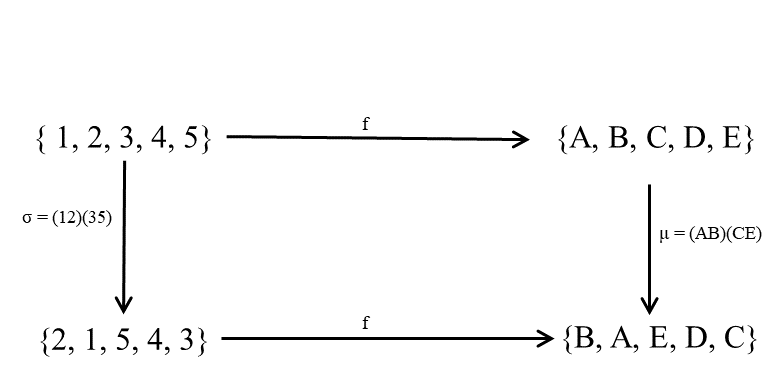
\includegraphics[width=3in]{images/Conj1a.png}
\caption{Conjugate mapping with $\sigma$ and $\mu$ permuting $\{1,2,3,4,5\}$.}
\end{center}
\end{figure}

\item
% $\sigma=(2346)$ and $f=\begin{pmatrix} 1&2&3&4&5&6\\ A&B&C&D&E&F \end{pmatrix}$
\begin{figure}[H]
\begin{center}
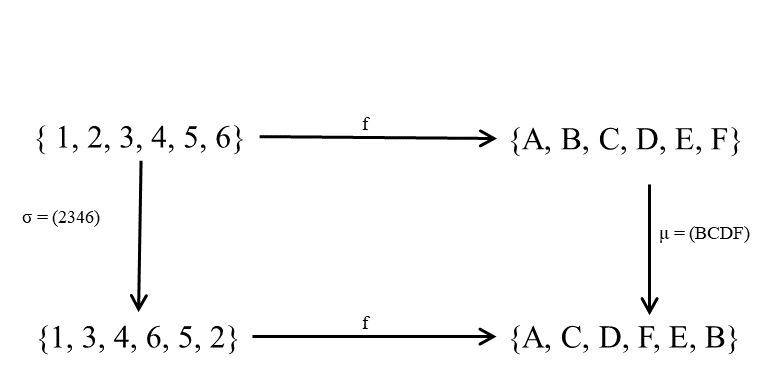
\includegraphics[width=3in]{images/Conj1b.png}
\caption{Conjugate mapping with $\sigma$ and $\mu$ permuting $\{1,2,3,4,5,6\}$.}
\end{center}
\end{figure}
\end{enumerate}

\noindent\textbf{Exercise \ref{exercise:actions:Conj3}}
%Given $\sigma$ and $\tau$ use the relabeling method to find the permutation conjugate to $\sigma$.  Check your work by computing $\tau\sigma\tau^{-1}$.
\begin{enumerate}[(a)]
\item 
%$\sigma=(6247)$ and $\tau=(527)(63)$.  $\sigma$ and $\tau$ act on the set $\{1,2,3,4,5,6,7\}$.
$\tau=\begin{pmatrix}1&2&3&4&5&6&7\\6&7&3&2&1&5&4
\end{pmatrix}$
\begin{align*}
\tau \circ \tau^{-1} &= (527)(63) \circ (6247) \circ (527)^2 (63)
\\
&= (527)(63) \circ (6247)\circ (257)(63)
\\
&= (527)(63) \circ (2563)(47)
\\
&= (3745)
\end{align*}

\item
%$\sigma=(256)(134)$ and $\tau=(21643)$.  $\sigma$ and $\tau$ act on the set $\{1,2,3,4,5,6\}$.
$\tau=\begin{pmatrix}1&2&3&4&5&6\\6&1&2&3&5&4
\end{pmatrix}$
\begin{align*}
\tau \circ \tau^{-1} &= (21643) \circ (256)(134) \circ (21643)^4
\\
&= (21643) \circ (256)(134) \circ (12346)
\\
&= (21643) \circ (1563)(24)
\\
&= (154)(236)
\end{align*}

\skipitems{1}
\end{enumerate}

\noindent\textbf{Exercise \ref{exercise:actions:Conj5}}
%In each of the following find a permutation $\tau$ that makes $\sigma$ and $\mu$ conjugate.  Check that $\sigma$ and $\mu$ are conjugate according to: $\mu = \tau \sigma \tau^{-1}$.

\begin{enumerate}[(a)]
\item
% $\sigma=(135)(792)(468)$, $\mu=(236)(189)(457)$
	\begin{multicols}{3}
	\begin{itemize}
	\item
	$1 \rightarrow 4$
	
	\item
	$2 \rightarrow 6$
	
	\item
	$3 \rightarrow 5$
	
	\item
	$4 \rightarrow 1$
	
	\item
	$5 \rightarrow 7$
	
	\item
	$6 \rightarrow 8$
	
	\item
	$7 \rightarrow 2$
	
	\item
	$8 \rightarrow 9$
	
	\item
	$9 \rightarrow 3$
	\end{itemize}
	\end{multicols}
$\tau = (14)(2689357)$
\\
check: $(14)(2689357)(135)(792)(468)(2753986)(14) = (189)(236)(457) = \mu$

\item
% $\sigma=(2879)(3561)$, $\mu=(2461)(5793)$
	\begin{multicols}{3}
	\begin{itemize}
	\item
	$1 \rightarrow 3$
	
	\item
	$2 \rightarrow 2$
	
	\item
	$3 \rightarrow 5$
	
	\item
	$4 \rightarrow 8$
	
	\item
	$5 \rightarrow 7$
	
	\item
	$6 \rightarrow 9$
	
	\item
	$7 \rightarrow 6$
	
	\item
	$8 \rightarrow 4$
	
	\item
	$9 \rightarrow 1$
	\end{itemize}
	\end{multicols}
$\tau = (135769)(48)$
\\
check: $(135769)(48)(2879)(3561)(48)(196753) = (1246)(3579) = \mu$

\skipitems{1}
\end{enumerate}

\noindent\textbf{Exercise \ref{exercise:actions:Conj7}}
%Complete the previous example with $G=D_4$ and $H=\{e,s\}$ by listing all the pairs $(h,g)$ with $h\in H$ and $g \in G$ together with the result of the mapping $hgh^{-1}$.  Simplify your expression for $hgh^{-1}$ as much as possible.
\\
$H = \{e, s\}$ and $G = \{e, r, r^2, r^3, s, s \circ r, s \circ r^2, s \circ r^3\}$
\begin{align*}
(h, g) &\implies hgh^{-1}
\\
(e, e) &\implies e \circ e \circ e^{-1} \implies e
\\
(e, r) &\implies e \circ r \circ e^{-1} \implies r
\\
(e, r^2) &\implies e \circ r^2 \circ e^{-1} \implies r^2
\\
(e, r^3) &\implies e \circ r^3 \circ e^{-1} \implies r^3
\\
(e, s) &\implies e \circ s \circ e^{-1} \implies s
\\
(e, s \circ r) &\implies e \circ s \circ r \circ e^{-1} \implies s \circ r
\\
(e, s \circ r^2) &\implies e \circ s \circ r^2 \circ e^{-1} \implies s \circ r^2
\\
(e, s \circ r^3) &\implies e \circ s \circ r^3 \circ e^{-1} \implies s \circ r^3
\\
(s, e) &\implies s \circ e \circ s^{-1} \implies e
\\
(s, r) &\implies s \circ r \circ s^{-1} \implies s \circ r \circ s \implies s \circ s \circ r^3 \implies r^3
\\
(s, r^2) &\implies s \circ r^2 \circ s^{-1} \implies s \circ r^2 \circ s \implies s \circ s \circ r^2 \implies r^2
\\
(s, r^3) &\implies s \circ r^3 \circ s^{-1} \implies s \circ r^3 \circ s \implies s \circ s \circ r \implies r
\\
(s, s) &\implies s \circ s \circ s^{-1} \implies s^2 \circ s \implies s
\\
(s, s \circ r) &\implies s \circ s \circ r \circ s^{-1} \implies r \circ s \implies s \circ r^3
\\
(s, s \circ r^2) &\implies s \circ s \circ r^2 \circ s^{-1} \implies r^2 \circ s \implies s \circ r^2
\\
(s, s \circ r^3) &\implies s \circ s \circ r^3 \circ s^{-1} \implies r^3 \circ s \implies s \circ r
\end{align*}

\noindent\textbf{Exercise \ref{exercise:actions:Conj8}}
%Fill in the blanks to prove the proposition:
%
%\noindent
%First, we have that $\underline{~<1>~}$ is in  $H$ and $e.g=\underline{~<2>~}g\underline{~<3>~} = g$.
%So the identity condition for a group action holds. 
%
%Also, observing that
%\[(h_1h_2).g =\underline{~<4>~}g\underline{~<5>~}
%= h_1(h_2g\underline{~<6>~} )\underline{~<7>~}
%= h_1. (\underline{~<8>~}. g)),\]
%we see that the compatibility condition is also satisfied.
\begin{multicols}{4}
\begin{enumerate}
\item
$e$

\item
$e$

\item
$e^{-1}$

\item
$h_1h_2$ 

\item
$(h_1h_2)^{-1}$

\item
$h_2^{-1}$

\item
$h_1^{-1}$

\item
$h_2$
\end{enumerate}
\end{multicols}

\noindent\textbf{Exercise \ref{exercise:actions:Conj15b}}
%Fill in the blanks to complete the proof that a group element and its conjugate always have the same order.
%
%Suppose that $\tilde{g}$ is conjugate to $g$. This means that there exists an $x\in G$ such that $\tilde{g}=\underline{~<1>~}$. Suppose $|g|=n$. Compute $\tilde{g}^n$ as follows:
%\begin{align*}
% \tilde{g}^n&=(\tilde{g} \ldots \tilde{g}~~~~~~~~~~~~(n~\text{ times)}\\ 
%&=(\underline{~<2>~}) \ldots (\underline{~<3>~})~~~~~~~~~~~~(n~\text{ substitutions)}\\ 
%& =xg(\underline{~<4>~})g \ldots g(\underline{~<5>~})gx^{-1}\qquad\text{(associative property)}\\
%&=xg(\underline{~<6>~})g...g(\underline{~<7>~})gx^{-1}\quad\text{( inverse property)}\\
%&=x(\underline{~<8>~})x^{-1}\quad\text{( identity property)}\\
%&=x(\underline{~<9>~})x^{-1}\quad\text{(definition of order)}\\
%&=\underline{~<10>~}\quad\text{(identity and inverse properties)}
%\end{align*}
%\noindent
%From Proposition~\ref{proposition:Groups:Cyclic_subgrp_order}, it follows that  $| \tilde{g}|$ divides $|\underline{~<11>~}|$. On the other hand, \[(\underline{~<12>~})\tilde{g}(\underline{~<13>~})=g\qquad\text{(inverse property)}.\]  
%The same proof  with $g$ and $\tilde{g}$ interchanged shows that $|g|$ divides $|\underline{~<14>~}|$ Therefore,  $|g|=\underline{~<15>~}$ 
\begin{multicols}{4}
\begin{enumerate}
\item
$xgx^{-1}$

\item
$xgx^{-1}$

\item
$xgx^{-1}$

\item
$x^{-1}x$

\item
$x^{-1}x$

\item
$e$

\item
$e$

\item
$g^n$

\item
$e$

\item
$e$

\item
$|g|$

\item
$x^{-1}$

\item
$x$

\item
$|\tilde{g}|$

\item
$|\tilde{g}|$
\end{enumerate}
\end{multicols}

\noindent\textbf{Exercise \ref{exercise:actions:Conj17}}
\begin{enumerate}[(a)]
\item
% Complete a conjugacy table like the one in  Example~\ref{example:actions:Conj16} for $G=D_4$. As in the example $r$ is a counterclockwise rotation by  $90^{\circ}$ and $s$ is the reflection that leaves the vertex labeled "1" fixed. Compute and simplify the conjugate expressions as compositions of $r$ and $s$. We show one row.  How many more rows are needed to complete the table?
%
%\begin{center}
%
%\begin{tabular}{ |r| c | c |c |c |c |c | c|c |} \hline
%  $g$ &$\var{id}$ & $r$ &$r^2$ &$r^3$ & $s$ &$s\compose r$ & $s\compose r ^2$ & $s\compose r^3$\\ \hline
%  $g\compose \var{id}\compose g^{-1}$ &--- & -- & -- &-- &--&--&--&-- \\
%\end{tabular}
%\end{center}
%
% Remember, once a group element appears in a row, you don't need to compute a row for that element, because you have already found its conjugacy class.
\begin{tabular}{ |r| c | c |c |c |c |c | c|c |} \hline
  $g$ &$\var{id}$ & $r$ &$r^2$ &$r^3$ & $s$ &$s\circ r$ & $s\circ r ^2$ & $s\circ r^3$\\ \hline
  $g\circ \var{id}\circ g^{-1}$ & $\var{id}$ & $\var{id}$ & $\var{id}$ & $\var{id}$ & $\var{id}$ & $\var{id}$ & $\var{id}$ & $\var{id}$ \\ \hline
  $g\circ r \circ g^{-1}$ & $r$ & $r$ & $r$ & $r$ & $r^3$ & $r^3$ & $r^3$ & $r^3$ \\ \hline
  $g\circ r^2 \circ g^{-1}$ & $r^2$ & $r^2$ & $r^2$ & $r^2$ & $r^2$ & $r^2$ & $r^2$ & $r^2$\\ \hline
  $g\circ s \circ g^{-1}$ & $s$ & $s \circ r^2$ & $s$ & $s \circ r^2$ & $s$ & $s \circ r^2$ & $s$ & $s \circ r^2$ \\ \hline
  $g\circ (s \circ r) \circ g^{-1}$ & $s \circ r$ & $s \circ r^3$ & $s \circ r$ & $s \circ r^3$ & $s \circ r^3$ & $s \circ r$ & $s \circ r^3$ & $s \circ r$ \\ \hline
\end{tabular}

\item 
%Verify that the class equation correctly calculates $|D_4|$.
$|D|_4| = 1 + 2 + 1 + 2 + 2 = 8$
\end{enumerate}

\noindent\textbf{Exercise \ref{exercise:actions:Conj21}}
%Let $G$ be an abelian group of finite order and $x,g\in G$.
%Simplify the conjugate expression $x\compose g\compose x^{-1}$.  How many conjugacy classes are in the abelian group $G$? How many elements are in each conjugacy class? 
\\
Since $G$ is abelian, 
\begin{align*}
x \circ g \circ x^{-1} &= x \circ x^{-1} \circ g &&\text{(commutative)}
\\
&= e \circ g &&\text{(inverse)}
\\
&= g &&\text{(identity)}
\end{align*}
The number of conjugacy classes is equal to $|G|$. There is only 1 element in each conjugacy class.

\section{Solutions for ``Polynomials''}
\noindent\textbf{\textit{ (Chapter \ref{poly})}}\bigskip

\noindent\textbf{Exercise \ref{exercise:poly:poly1}}
\begin{enumerate} [(a)]
\item
 Sum: $x^3$ , Product: $x^5+x^3+x^2+1$
\item
 Sum: $x^3+1$ , Product: $x^8+x^7+x^5+x^3+x^2$
\item
 Sum: $0$ , Product: $x^8+x^6+x^4+x^2+1$
\end {enumerate}

\noindent\textbf{Exercise \ref{exercise:poly:poly2}}
\begin{enumerate} [(a)]
\item
 $\mathbb{Z}[x]$,$\mathbb{Q}[x]$,$\mathbb{R}[x]$,$\mathbb{C}[x]$,$\mathbb{Z}_5[x]$,$\mathbb{Z}_6[x]$
\item
 None
\item
 $\mathbb{Q}^*[x],\mathbb{R}^*[x], \mathbb{C}^*[x], {\mathbb{Z}_5}^*[x]$
\item
 None
\end {enumerate}

\noindent\textbf{Exercise \ref{exercise:poly:poly3l}}
\begin{enumerate} [(a)]
\item
 Sum: $x^3+x+1$ , Product: $2x^5+2x^4+4x^3+3x^2$
\item
 Sum: $2x^4+4x^3$ , Product: $2x^7+x^6+4x^5+4x^3+4x^2+5$
\end {enumerate}

\noindent\textbf{Exercise \ref{exercise:poly:poly4}}
\begin{enumerate} [(a)]
\item
 $\sum_{i=0}^{4} (2i+1)x^2i$, degree: 8
\item
 $\sum_{i=0}^{3} \cis(i\pi/2)x^2i$, degree: 6
\item 
$\sum_{i=0}^{3} (7i^3-18i^2+13i+1)x^i$, degree: 3
\item
 $\sum_{i=0}^{5} ((-1)^i/(2i+1))x^i$, degree: 5
\end {enumerate}

\noindent\textbf{Exercise \ref{exercise:poly:poly5}}
\begin{enumerate} [(a)]
\item
 No
\item 
Yes
\item
 n is a prime number.
\end {enumerate}

\noindent\textbf{Exercise \ref{exercise:poly:poly6}}
\begin{enumerate} [(a)]
\item
 $p(x)=2x$, $q(x)=2x^3+2$
\item 
No
\item
 $p(x) \cdot q(x)=0$, where $p(x)=3x^3$ and $q(x)=2x^2$ are in $\mathbb{Z}_6[x]$.
\end {enumerate}

\noindent\textbf{Exercise \ref{exercise:poly:mult2way}}
\begin{enumerate} [(a)]
\item 
 $x^3-2x^2-15x$
\item
 $5x^4-5\sqrt{3}x^2+2\sqrt{3}x-6$
\item
$4x^5-3x^4+\frac{7}{2}x^3+8x^2-6x+7$
\item
$80x^7-40x^6+64x^5-90x^4+47x^3-21x^2$
\end {enumerate}

\noindent\textbf{Exercise \ref{exercise:poly:multform}}
\begin{enumerate} [(a)]
\item 
 $x^6+2x^5+3x^4+4x^3+3x^2+2x+1$
\item
 $2x^5+5x^4+8x^3+3x^2$
\item
$2x^8+x^7-2x^6-6x^5-10x^4-2x^3+4x^2+7x+6$
\item
$12x^8+6x^7-12x^6-36x^5-60x^4-12x^3+24x^2+42x+36$
\end {enumerate}

\noindent\textbf{Exercise \ref{exercise:poly:div1}}
\begin{enumerate} [(a)]
\item 
 $q(x)=x+5$, $r(x)=37$
\item
 $q(x)=15x^2+75x+388$, $r(x)=1913$
\item
$q(x)=5x-\frac{1}{2}$, $r(x)=23x+25$
\end {enumerate}

\noindent\textbf{Exercise \ref{exercise:poly:div2}}
\begin{enumerate} [(a)]
\item
$3x^5 + 2x^4 + 3x^3 + x^2 +2x +4$
\item
$x^6 + x^5 + x^2 + x$
\item
$4x^4 + 6x^3 + 2x^2 + 1$
\item
$x^3+2x^2+5x+4$
\end {enumerate}

\noindent\textbf{Exercise \ref{exercise:poly:complexPoly}}
\begin{enumerate} [(a)]
\item
$(x+1)(x-3-2i)(x-3+2i)$
\end {enumerate}


%\end {answer}



%
%\backmatter
%% bibliography, glossary and index would go here.
%
%\end{document}


\section{Solutions for ``Induction''}
\subsection{Proofs for Section~\ref{sec:basic_induction}}
\subsubsection{Induction proofs, type I: sum/product formulas}


\textbf{Proof of (a):}
We seek to show that, for all $n\in\NN$,  
\[
\sum_{i=1}^n i(i+1)=\frac{n(n+1)(n+2)}{3}. 
\tag{$*$}
\]

\textbf{Base case:} When $n=1$, the left side of ($*$) is $1\cdot(1+1) =2$,
and the
right side is $1\cdot(1+1)(1+2)/3=2$, so both sides are equal and ($*$) is
true for $n=1$.

\textbf{Induction step:} Let $k\in\NN$ be given and suppose 
($*$) is true for $n=k$. Then
\begin{align*}
\sum_{i=1}^{k+1}i(i+1)
&=
\sum_{i=1}^{k}i(i+1)
+(k+1)(k+2)
\\
&=\frac{k(k+1)(k+2)}{3} 
+(k+1)(k+2)
\quad \text{(by induction hypothesis)}
\\
&=\frac{(k+1)(k+2)(k+3)}{3}.
\end{align*}
Thus, ($*$) holds for $n=k+1$, and the proof of the induction step is complete. 

\textbf{Conclusion:} By the principle of induction,  it follows that
($*$) is true for all $n\in\NN$.  
\medskip
We furnish no proofs for (b) and (c).  Note that (b) is a special case of (c).

\medskip


\textbf{Proof of (d):}
We seek to show that, for all $n\in\NN$,
\[
\sum_{i=0}^n i! i
= (n+1)!-1. 
\tag{$*$}
\]

\textbf{Base case:} When $n=1$, the left side of ($*$) is $0+1 \cdot 1! =1$,
and the
right side is $(1+1)!-1=1$, so both sides are equal and ($*$) is
true for $n=1$.

\textbf{Induction step:} Let $k\in\NN$ be given and suppose 
($*$) is true for $n=k$. Then
\begin{align*}
\sum_{i=1}^{k+1}i\cdot i!
&=
\sum_{i=1}^{k}i\cdot i! + (k+1)(k+1)!
\\
&= (k+1)!-1 + (k+1)(k+1)!
\quad \text{(by induction hypothesis)}
\\
&=(k+1)!(k+2)-1
\\
&=(k+2)!-1.
\end{align*}
Thus, (2) holds for $n=k+1$, and the proof of the induction step is complete. 

\textbf{Conclusion:} By the principle of induction, 
($*$) is true for all $n\in\NN$.  

\subsubsection{Induction proofs, type II: Inequalities}

We will give detailed proofs for (c), (d), (e). The other inequalities can
be proved similarly.

\medskip

\textbf{Proof of (c):}
A direct check of the inequality for the first few values of $n$ shows
that the left-right pairs in the stated inequality 
are $(1,2),(2,4),(6,8),(24,16),(120,32)$. Thus, the inequality
fails for $n=1,2,3$, but holds for $n=4,5$. This suggests that it indeed
holds for all $n$ from $4$ onwards. We will prove this by induction,
i.e., we will show that 
\[
n!>2^n
\tag{$*$}
\]
holds for all $n\ge4$.

\textbf{Base case:} For $n=4$, the left and right sides of ($*$) are 
$24$ and $16$, respectively, so ($*$) is true in this case. 

\textbf{Induction step:} Let $k\ge4$ be given and suppose 
($*$) is true for $n=k$. Then
\begin{align*}
(k+1)!&=k!(k+1)
\\
&>2^k(k+1)
\quad \text{(by induction hypothesis)}
\\
&\ge 2^k\cdot 2
\quad \text{(since $k\ge4$ and so $k+1\ge2$))}
\\
&=2^{k+1}.
\end{align*}
Thus, ($*$) holds for $n=k+1$, and the proof of the induction step is complete. 

\textbf{Conclusion:} By the principle of induction, 
it follows that ($*$) is true for all $n\ge4$.  

\bigskip

\textbf{Proof of (d) and (e):}
We will prove that for any real number $x>-1$  
\[
(1+x)^n\ge 1+nx.
\tag{$*$}
\]
holds for any $n\in\NN$.
This simultaneously proves both statements (d) and (e): (e) corresponds
to the case $x>0$, while (d) corresponds to the case $-1<x<0$ (with
$x'=-x$ in place of $x$).

\textbf{Base case:} For $n=1$, the left and right sides of ($*$) are 
both $1+x$, so ($*$) holds.

\textbf{Induction step:} Let $k\in\NN$ be given and suppose ($*$) is true
for $n=k$ and any real number $x>-1$.   We seek to show that ($*$) holds
for $n=k+1$ and any real number $x>-1$.

Let $x>-1$ be given. Then
\begin{align*}
(1+x)^{k+1}
&=(1+x)^k(1+x)
\\
&\ge (1+kx)(1+x) 
\quad\text{(by ind. hyp. and since $x>-1$ and thus $(1+x)>0$)}
\\
&=1+(k+1)x +kx^2
\quad\text{(by algebra)}
\\
&\ge 1+(k+1)x 
\quad\text{(since $kx^2\ge0$)}.
\end{align*}
Hence ($*$) holds for $n=k+1$, and the proof of the induction step is
complete.

\textbf{Conclusion:} By the principle of induction, it follows that ($*$)
holds for all $n\in\NN$.

\subsubsection{Induction proofs, type III:
Extension of theorems from $2$ variables to $n$ variables}

We will prove by induction on $n$ the following statement: 

\[
\tag*{$P(n)$:}
\parbox{5in}{\slshape For all real numbers $a_i$ and $b_i$ ($i=1,\dots,n$)
such that $a_i\le b_i$ for all $i$ we
have}
\]
\[
\sum_{i=1}^na_i\le \underline{~~~~~~~}. 
\tag{$*$}
\]
(Note that the condition ``for all real numbers $a_i$ and $b_i$''
must be part of the induction statement we seek to prove.)

\textbf{Base case:} For $n=1$, the 
left and right sides are \underline{~~~} and \underline{~~~~}, respectively, and the
inequality ($*$) therefore follows from our hypothesis that
$a_i\le b_i$ for all $i=1,\dots,n$.  Hence \underline{~~~~} is true.

\textbf{Induction step:}
\begin{itemize}
\item Let $k\ge 1$, and suppose $P(k)$ is true, i.e.,
suppose that 
for $n=$\underline{~~~} and any choice of real numbers 
$a_1,\dots,a_k$ and $b_1,\dots,b_k$ 
satisfying \underline{~~~~} for each $i$, the inequality ($*$) holds.
\item
We seek to show that \underline{~~~} is true, i.e., that 
for $n=$\underline{~~~~}
any choice of real numbers $a_1,\dots,a_{k+1}$ and $b_1,\dots,b_{k+1}$
satisfying \underline{~~~~~} for each $i$, the inequality ($*$) holds.
\item
Let $a_1,\dots,a_{k+1}$ and $b_1,\dots,b_{k+1}$ be given real numbers
such that \underline{~~~~~} for each $i$.
\item Then
\begin{align*}
\sum_{i=1}^{k+1}a_i
&=\underline{~~~~~} + a_{k+1}
\\
&\le \underline{~~~~~~} + a_{k+1}
\quad \text{(by induction hypothesis applied to $a_1,\dots a_k$)}
\\
&\le \sum_{i=1}^{k}b_i + \underline{~~~~~}
\quad \text{(by assumption $a_{k+1}\le b_{k+1}$)}
\\
&=\sum_{i=1}^{k+1}b_i.
\end{align*}
\item 
Thus, ($*$) holds for $n=$\underline{~~~~} and the given numbers $a_1,\dots,a_{k+1}$ 
and $b_1,\dots,b_{k+1}$.
\item Since the $a_1,\dots,a_{k+1}$ 
and $b_1,\dots,b_{k+1}$ were arbitrary
real numbers satisfying $a_i\le b_i$ for each $i$,
we have obtained statement $P(k+1)$, 
and the proof of the induction step is complete.
\end{itemize}


\textbf{Conclusion:} By the principle of induction, 
it follows that $P(n)$ is true for all $n\in\NN$.  
  {\hspace\fill$\square$\par\medskip}

We seek to prove by induction on $n$ the following statement: 
\[
\tag*{$P(n)$:}
\parbox{5in}{\slshape For all real numbers $x_1,\dots,x_n$ 
we have}
\]
\[
\left|\sin\left(\sum_{i=1}^n x_i\right)\right|
\le \sum_{i=1}^n\left|\sin x_i\right|.
\tag{$*$}
\]

The key to the argument is the trig identity
\[
\sin(\alpha+\beta)=\sin\alpha \cos \beta+\sin\beta\cos\alpha,
\]
which is valid for any real $\alpha$ and $\beta$. Since $|\cos x|\le 1$,
this identity implies, via the triangle inequality,
\begin{align*}
\tag{$**$}
|\sin(\alpha+\beta)|
&\le|\sin\alpha \cos \beta|+|\sin\beta\cos\alpha|
\\
&\le|\sin\alpha|+|\sin\beta|.
\end{align*}
The inequality $(**)$ is the case $n=2$ of the statement $(*)$ 
we seek to prove, and will be needed in the induction proof. (One could
also use it as the base case of an induction proof that starts with $n=2$, 
but it is easier to start the induction with $n=1$, where the base case
is trivial.)

\bigskip


\textbf{Base case:} For $n=1$, the 
left and right sides of ($*$) are both equal to $|\sin x_1|$, so  
($*$) holds trivially in this case. Hence $P(1)$ is true.

\textbf{Induction step:}
\begin{itemize}
\item Let $k\ge 1$, and suppose $P(k)$ is true, i.e.,
suppose that ($*$) holds for $n=k$ and any choice of real numbers 
$x_1,\dots,x_k$.
\item
We seek to show that $P(k+1)$ is true, i.e., that for
any choice of real numbers $x_1,\dots,x_{k+1}$
the inequality ($*$) holds. 
\item
Let $x_1,\dots,x_{k+1}$  be given real numbers. 
\item Then
\begin{align*}
\left|\sin\left(\sum_{i=1}^{k+1} x_i\right)\right|
&=\left|\sin\left(\left(\sum_{i=1}^{k} x_i\right) + x_{k+1}\right)\right|
\\
&\le \left|\sin\left(\sum_{i=1}^{k} x_i\right)\right|
+ \left|\sin x_{k+1}\right|
\quad \text{(by ($**$)
with $\alpha=\sum_{i=1}^k x_i$ and $\beta=x_{k+1}$)}
\\
&\le \sum_{i=1}^k\left|\sin x_i\right|
+ \left|\sin x_{k+1}\right|
\quad \text{(by induction hypothesis applied to $x_1,\dots, x_k$)}
\\
&=\sum_{i=1}^{k+1}\left|\sin x_i\right|.
\end{align*}
\item 
Thus, ($*$) holds for $n=k+1$ and the given numbers $x_1,\dots,x_{k+1}$.
\item
Since the $x_1,\dots,x_{k+1}$ were
arbitrary real numbers, we have obtained statement $P(k+1)$, and 
proof of the induction step is complete.
\end{itemize}

\textbf{Conclusion:} By the principle of induction, 
it follows that $P(n)$ is true for all $n\in\NN$.  

We seek to prove by induction on $n$ the following statement: 
\[
\tag*{$P(n)$:}
\parbox{5in}{\slshape For all sets $A_1,\dots,A_n$  
we have}
\]
\[
\left(A_1\cup \dots \cup A_n\right)^c
=A_1^c\cap\dots \cap A_n^c.
\tag{$*$}
\]

The key to the argument is two set version of De Morgan's Law:
\[
(A\cup B)^c = A^c\cap B^c,
\tag{$**$}
\]
which holds for any sets $A$ and $B$.


\textbf{Base case:} For $n=1$, the 
left and right sides of ($*$) are both equal to $A_1^c$,
so ($*$) holds trivially in this case. Hence $P(1)$ is true.
\iffalse
Though not necessary, we can also easily verify the next case,
$n=2$: In this case, the left and right sides of ($*$) are $(A_1\cup A_2)^c$
and $A_1^c\cap A_2^c$, respectively, so the identity is just the two set
version of De Morgan's Law, i.e., ($**$) with $A=A_1$ and $B=A_2$.
\fi

\textbf{Induction step:} 
\begin{itemize}
\item Let $k\ge 1$, and suppose $P(k)$ is true, i.e.,
suppose that ($*$) holds for $n=k$ and any sets $A_1,\dots,A_k$.
\item
We seek to show that $P(k+1)$ is true, i.e., that for
any sets $A_1,\dots,A_{k+1}$, ($*$) holds. 
\item
Let $A_1,\dots,A_{k+1}$  be given sets.
\item
Then
\begin{align*}
\left(A_1\cup \dots \cup A_{k+1}\right)^c
&=\left(\left(A_1\cup \dots \cup A_{k}\right)\cup A_{k+1}\right)^c
\\
&=\left(A_1\cup \dots \cup A_{k}\right)^c\cap A_{k+1}^c
\quad\\
& \qquad \qquad\qquad \text{(by ($**$) with $A=(A_1\cup \dots \cup A_k)$ and 
$B=A_{k+1}$)}
\\
&=\left(A_1^c\cap\dots \cap A_k^c\right)\cap A_{k+1}^c\\
& \qquad \qquad\qquad \text{(by induction hypothesis applied to $A_1,\dots, A_k$)}
\\
&=A_1^c\cap\dots \cap A_k^c\cap A_{k+1}^c.
\end{align*}
\item
Thus, ($*$) holds for $n=k+1$
and the given sets $A_1,\dots,A_{k+1}$.
\item 
Since the $A_1,\dots,A_{k+1}$ were
arbitrary sets, we have obtained statement $P(k+1)$, and the 
proof of the induction step is complete.
\end{itemize}

\textbf{Conclusion:} By the principle of induction, 
it follows that $P(n)$ is true for all $n\in\NN$.  
 

\subsection{Proofs for Section~\ref{sec:Induction:StrongInductionPractice}}
\subsubsection{``Strong induction and recurrences''}

\noindent
\textbf{Proof of (a):}

We seek to show that, for all $n\in\NN$, 
\[
\tag{$*$}
\sum_{i=1}^n F_i=F_{n+2}-1.
\]

\textbf{Base case:} When $n=1$, the left side of ($*$) is $F_1 =1$,
and the
right side is $F_3-1=2-1=1$, so both sides are equal and ($*$) is
true for $n=1$.

\textbf{Induction step:} Let $k\in\NN$ be given and suppose 
($*$) is true for $n=k$. Then
\begin{align*}
\sum_{i=1}^{k+1}F_i
&=
\sum_{i=1}^{k}F_i
+F_{k+1}
\\
&=F_{k+2}-1 + F_{k+1}
\quad \text{(by ind. hyp. $(*)$ with $n=k$)}
\\
&=F_{k+3}-1 
\quad \text{(by recurrence for $F_n$)}
\end{align*}
Thus, ($*$) holds for $n=k+1$, and the proof of the induction step is complete. 

\textbf{Conclusion:} By the principle of induction,  it follows that
($*$) is true for all $n\in\NN$.  

\bigskip

\textbf{Remark:} Here standard induction was sufficient, since we were
able to relate the $n=k+1$ case directly to the $n=k$ case, in the
same way as in the induction proofs for summation formulas like 
$\sum_{i=1}^n i=n(n+1)/2$.  Hence, a single base case was sufficient.

(For convenience, we define $F_0=0$; with this definition, the recurrence
relation $F_n=F_{n-1}+F_{n-2}$ holds for all $n\ge2$ and the above matrix
is well defined for all $n\ge1$.)

\textbf{Base case:} When $n=1$, 
the four entries of the matrix on the right are $F_2=1$, $F_1=1$, $F_1=1$, 
and $F_0=0$, so ($*$) holds in this case. 

\newcommand{\mat}[4]{\begin{pmatrix}#1 & #2 \\ #3 & #4\end{pmatrix}}
\textbf{Induction step:} Let $k\in\NN$ be given and suppose 
($*$) holds for $n=k$. Then
\begin{align*}
\mat 1110^{k+1}
&=\mat 1110^k\mat1110
\\
&=\mat{F_{k+1}}{F_k}
{F_k}{F_{k-1}}\mat1110
\quad\text{(by $(*)$ with $n=k$)}
\\
&=\mat{F_{k+1}+F_k}{F_{k+1}}{F_{k}+F_{k-1}}{F_k}
\quad \text{(by matrix multiplication)}
\\
&=\mat{F_{k+2}}{F_{k+1}}{F_{k+1}}{F_k}
\quad \text{(by recurrence for $F_n$)}.
\end{align*}
Thus, ($*$) holds for $n=k+1$, and the proof of the induction step is complete. 

\textbf{Conclusion:} By the principle of induction,  it follows that
($*$) is true for all $n\in\NN$.  

\textbf{Proof of (b):}

We will use induction to show that the following statement 
holds for all $m\in\NN$:
\[
\tag*{$P(m):$}
\text{
$F_{3m-2}$ and $F_{3m-1}$ are odd,
and $F_{3m}$ is even.}
\]

\textbf{Base case:} When $m=1$, the three Fibonacci numbers appearing in 
$P(m)$ are $F_1=1$, $F_2=1$, and $F_3=2$, and thus are of the required
parity. Hence $P(1)$ is true.

\textbf{Induction step:} Let $k\in\NN$ be given and suppose 
$P(m)$ is true for $m=k$. Thus, $F_{3k-2}$ and $F_{3k-1}$ are odd and 
$F_{3k}$ is even.

By the recurrence for $F_n$, we have $F_{3k+1}=F_{3k}+F_{3k-1}$. Hence
$F_{3k+1}$ is the sum of an even number $F_{3k}$, and an odd number,
$F_{3k-1}$, and therefore odd. 

Similarly, $F_{3k+2}=F_{3k+1}+F_{3k}$, so $F_{3k+2}$ is the sum of an odd
number, $F_{3k+1}$, and an even number, $F_{3k}$, and hence odd.

Finally, $F_{3k+3}=F_{3k+2}+F_{3k+1}$, so $F_{3k+3}$ is the sum of two odd
numbers and hence even. 

Altogether, we have shown that, of the three numbers
$F_{3k+1},F_{3k+2},F_{3k+3}$, the first two are odd and the last one is
even. Thus $P(m)$ holds for $m=k+1$, and the proof of the 
induction step is complete. 

\textbf{Conclusion:} By the principle of induction,  it follows that
$P(m)$ is true for all $m\in\NN$.  

\bigskip

\textbf{Alternative argument:} The above proof lumps together groups of
three consecutive Fibonacci numbers and establishes the desired parity
properties simultaneously for all three numbers.  
Alternatively, one can treat the sequences $F_{3m-2}$, $F_{3m-1}$, and
$F_{3m}$ separately using  the following identity, valid for 
all $n\ge4$:
\[
F_{n}=F_{n-1}+F_{n-2}=(F_{n-2}+F_{n-3})+F_{n-2}=2F_{n-2}+F_{n-3}.
\]
It follows from this identity that if $F_{n-3}$ is odd, then so is $F_{n}$,
and if $F_{n-3}$ is even, then so is $F_n$.  Using 
induction with $n=1$ as the base case then shows that the numbers
$F_1=1,F_4,F_7,\dots$ are all odd.  With $n=2$ as base case one gets that 
$F_2=1,F_5,F_8,\dots$ are all odd, and taking $n=3$ as base case 
shows that $F_3=2,F_6,F_9,\dots$ are all even.


\textbf{Proof of (c):}
We will prove $(*)$ by strong induction.

\textbf{Base step:} 
For $n=1,2,3$, $T_n$ is equal to $1$, whereas the
right-hand side of ($*$) is equal to $2^1=2$, $2^2=4$, and $2^3=8$,
respectively. Thus, ($*$) holds for $n=1,2,3$.

\textbf{Induction step:} Let $k\ge3$ be given and suppose 
($*$) is true for all $n=1,2,\dots,k$. Then
\begin{align*}
T_{k+1}&=T_{k}+T_{k-1}+T_{k-2}
\quad \text{(by recurrence for $T_n$)}
\\
&<2^{k}+2^{k-1}+2^{k-2} \quad \text{(by strong ind. hyp. ($*$)
with $n=k$, $k-1$, and $k-2$)}
\\
&=2^{k+1}\left(\frac12+\frac14+\frac18\right)
\\
&=2^{k+1}\frac{7}{8}
<2^{k+1}.
\end{align*}
Thus, ($*$) holds for $n=k+1$, and the proof of the induction step is complete. 

\textbf{Conclusion:} By the strong induction principle,  it follows that
($*$) is true for all $n\in\NN$.  

\subsubsection{Strong induction and representation problems}

\textbf{Proof of (a):}

A quick direct check shows that the 
positive numbers $n<15$ that have a
representation $n=3x+7y$ with $x,y\in\NN\cup \{0\}$) are exactly
$3,6,7,9,10,12,13,14$.  We now use strong induction to show that from
$12$ onwards every integer has a representation in the above form.
In other words, we will prove that the following 
statement holds for all $n\ge12$:
\[
\text{$n$ has a representation $(*)$ $n=3x+7y$ with $x,y\in\NN\cup \{0\}$}
\tag{$P(n)$}
\]
\textbf{Base case:} For $n=12,13,14$, the representations $12=3\cdot 4$,
$13=3\cdot 2+7$ and $14=7\cdot 2$ show that $P(n)$ is true.

\textbf{Induction step:} 
Let $k\ge14$ be given and suppose $P(k')$ is true for all $k'$ with 
$k'=12,13,\dots,k$, i.e., suppose that all such $k'$ have a representation in
the form $(*)$. We seek to show that $k+1$ also has a representation of
this form. 

Write  $k+1=3+k'$, so that $k'=k-2$. Note that $k'\le k$ and  also
$k'\ge 12$ since we assumed $k\ge14$. Thus, we can apply the strong
induction hypothesis to $k'$ and obtain a representation 
\[
k'=3x+7y,
\]
where $x,y\in\NN\cup\{0\}$. Adding $3$ to both sides of this
representation, we get
\[
k+1=k'+3= 3x+7y+3=3(x+1)+7y,
\]
which is a representation of the desired form for $k+1$.
Hence $P(k+1)$ is true, and the proof of the induction step is complete.

\textbf{Conclusion:} By the strong induction principle, 
it follows that $P(n)$  is true for all $n\ge12$.

\bigskip

\textbf{Remark:} Note that, in the induction step, in order to be able
to apply the induction hypothesis with $k'=k-2$ we need to ensure that 
$k'$ is at least $12$. This in turn requires $k$ 
to be at least $14$ in the induction step,
and the cases $k=12,13,14$ to be treated as base
cases.


\textbf{Proof of (b):}
We will prove by strong induction that the following statement  
holds for all $n\in\NN$:

\[\text{$n$ has a representation}(*) ~~n=2^{i_1}+\dots + 2^{i_h} \]
\[ \text{with distinct integers $i_1,\dots,i_h\in\NN\cup\{0\}$.}
\tag{$P(n)$}
\]
\textbf{Base case:} The integer $n=1$ has the representation $1=2^0$,
which is of the desired form. Hence $P(n)$ holds for $n=1$.


\textbf{Induction step:} 
Let $k\ge1$ be given and suppose $P(n)$ is true for all positive
integers $ n\le k$, i.e., suppose that all such $n$ have a
representation in the form $(*)$. We seek to show that $n=k+1$ also has a
representation of this form. 

Let $2^m$ be the largest (integer) power of $2$ that satisfies $2^m\le k+1$.

If $2^m=k+1$, then $k+1$ has a representation of the desired form
(namely as a sum of a single power of $2$, $2^m$), and we are done.

If $2^m<k+1$, we let $k'=k+1-2^m$.  Since $2^m\ge1$
and $2^m<k+1$, $k'$ is an integer with $1\le k'\le k$. 
Hence we can apply the strong induction hypothesis to $k'$ and obtain a
representation of $k'$ as a sum of distinct powers of $2$.

Adding $2^m$ to this representation gives a representation of $k+1=k'+2^m$
as a sum of powers of $2$. To complete the proof of the induction step,
we still need to show that the powers of $2$ involved here are distinct.

Since the powers of $2$ representing $k'$ were already distinct, it
suffices to show that the added power $2^m$ cannot occur among the
powers in the representation for $k'$. 
To do this, we exploit the fact that $2^m$ was chosen as the largest
power of $2$ below $k+1$. Thus, we have
\[
2^m< k+1 < 2^{m+1}.
\]
Subtracting $2^m$ from both sides, we get 
\[
0< k+1-2^m<2^{m+1}-2^m=2^m,
\]
and since $k'=k+1-2^m$, it follows that $k'$ is strictly less than
$2^m$, and so $2^m$ cannot occur in the representation for $k'$.
This is what we wanted to show.

Thus, the representation for $k+1$ that we obtained is indeed a
representation of the desired form and the proof of the 
induction step is complete.

\textbf{Conclusion:} By the strong induction principle, 
it follows that $P(n)$  is true for all $n\ge1$.

\bigskip

\textbf{Remarks:} The argument used above in the induction step is called a
``greedy'' algorithm: In constructing a binary representation for $k+1$, one
starts  out by using the largest possible ``building block'' (namely, the
largest power of $2$ that is $\le k+1$), and then uses the strong induction
hypothesis to make up for the left over part. 


An alternative, but less flexible, approach to the induction step is as
follows: If $k+1$ is even, then $k+1=2k'$, where $k'$ is an integer in
the range $1\le k'\le k$. By the strong induction hypothesis $k'$
has a representation as sum of distinct powers of $2$, and multiplying this
representation by $2$ gives a representation of the desired form for $k+1$. 
If $k+1$ is odd, a similar argument based on the representation $k+1=2k'+1$
yields the same conclusion. 

The latter approach, however, relies heavily on specific arithmetic properties
of the powers of $2$ and does not generalize to other sequences like Fibonacci
numbers or factorials. By contrast, the ``greedy'' approach is one that can be
used for many representation problems and, in fact, is the standard way to
handle such problems.

\bigskip

\textbf{Uniquess of representation:} The above argument proves only the
\emph{existence} of a representation, not its uniqueness.  One way to prove the
uniqueness is by contradiction: Assume there are positive integers with
multiple representations, let $n$  be the smallest of these exceptional
integers, and derive a contradiction from this assumption.

Another way to prove uniquess is to incorporate the uniqueness claim into the
statement $P(n)$ to be proved. The strengthened statement requires an additional
argument in the induction step showing that uniqueness holds for $k+1$,
provided it holds for all $k'\le k$. This is not difficult; the key observation
is that any representation of $k+1$ must necessarily involve the power $2^m$ 
defined above.

\textbf{Proof of (c):}
We will prove by strong induction that the following statement  
holds for all $n\in\NN$.
\[
\text{$n$ has a representation 
$(*)$ $\sum_{i=1}^rd_ii!$
with $d_i\in\{0,1,\dots,i\}$.}
\tag{$P(n)$}
\]
\textbf{Base case:} The integer $n=1$ has the representation $1=1\cdot 1!$,
which is of the desired form. Hence $P(n)$ holds for $n=1$.


\textbf{Induction step:} 
Let $k\ge1$ be given and suppose $P(n)$ is true for all positive
integers $ n\le k$, i.e., suppose that all such $n$ have a
representation in the form $(*)$. We seek to show that $n=k+1$ also has a
representation of this form. 

Let $r$ be the \emph{largest} integer such that $r!\le k+1$; i.e., $r$ is the
unique integer for which  
\[
r!\le k+1 < (r+1)!.
\tag{1}
\]

If $r!=k+1$, then $k+1$ has a representation of the desired form,
and we are done.

If $r!<k+1$, we let $k'=k+1-r!$.  Since $1\le r!<k+1$, 
$k'$ is an integer in the range $1\le k'\le k$. 
Hence we can apply the strong induction hypothesis to $k'$ and obtain a
representation of $k'$ as a finite sum of terms $d_ii!$, with ``digits'' 
$d_i$ in the range $0\le d_i\le i$.  

Adding $r!$ to this representation gives a representation of $k+1=k'+r!$
as a sum of factorials.  To complete the induction step, we need to make sure
that this new representation still satisfies the constraints $0\le d_i\le i$ 
on the digits. 

If $r!$ does not occur in the representation of $k'$, this is clearly the case.

If $r!$ does occur in the representation of $k'$ with an associated
``digit'' $d_r$ satisfying $d_r\le r-1$, 
then adding $r!$ to this representation gives a
representation with $d_r$ replaced by $d_r+1$ and all other digits unchanged, 
and since $d_r\le r-1$, the new digit $d_r+1$ satisfies the required
constraint, $d_r+1\le r$.

It remains to consider the case when $k'$ has a representation involving $r!$
in which the associated digit is maximal, i.e., $d_r=r$. But then 
\[
k+1=k'+r!\ge d_rr!+r! =r\cdot r! + r!=(r+1)!,
\]
so $(r+1)!\le k+1$, contradicting (1). Therefore this case is impossible. 

Hence, in each case we have obtained a representation of $k+1$ of the 
desired form and the proof of the 
induction step is complete.

\textbf{Conclusion:} By the strong induction principle, 
it follows that $P(n)$  is true for all $n\ge1$.

\subsection{Proofs for Section~\ref{practice_non_formula}}

\textbf{Proof of (a):}
We use a variation of the above argument (showing that an
$n$-element set has $2^n$ subsets).  For brevity, we call a subset with an odd
number of elements an ``odd subset'', and a subset with an even number of
elements an ``even subset.'' 

Let $P(n)$ denote the statement that \textbf{any set with $n$ elements has
$2^{n-1}$ odd subsets and $2^{n-1}$ even subsets.}
We use induction to show that $P(n)$ holds for all $n\in\NN$.

\textbf{Base case:} A $1$-element set $A=\{a_1\}$ has exactly 
one even subset, the empty set $\emptyset$ (since the empty set has $0$
elements, and $0$ is an even number), and one odd subset, $\{a_1\}$, so $P(1)$
is true.

\textbf{Induction step:} 
Let $k\in\NN$ be given and suppose 
$P(k)$ is true, i.e., that any $k$-element set has $2^{k-1}$ even subsets and
$2^{k-1}$ odd subsets. 
We seek to show that $P(k+1)$  is true as well, i.e., that
any $(k+1)$-element set has $2^{k}$ even subsets and $2^k$ odd subsets.

Let $A$ be a set with $(k+1)$ elements.  
Choose an element $a$ in $A$, and set $A'=A-\{a\}$. 

We again classify the subsets of $A$ into two types: (I) subsets that do
\emph{not} contain $a$, and (II) subsets that do contain $a$.
The subsets of type (I) are exactly the subsets of the set
$A'$. Since $A'$ has $k$ elements, the induction
hypothesis can be applied to this set and we get that there are 
$2^{k-1}$ even subsets and $2^{k-1}$ odd subsets of type (I).

The subsets of type (II) are exactly the sets of the form $B=B'\cup
\{a\}$, where $B'$ is a subset of $A'$, and hence are in one-to-one
correspondence with subsets $B'$ of $A'$.  Moreover, $B$ is
an odd subset of
$A$ if and only if the associated set $B'$ is an even subset of $A'$,
and an even subset of
$A$ if and only if the associated set $B'$ is an odd subset of $A'$.
By the
induction hypothesis there are $2^{k-1}$ even subsets of $A'$, and $2^{k-1}$
odd subsets of $A'$.   Hence there are $2^{k-1}$ odd subsets of type (II), and
$2^{k-1}$ even subsets of type (II).

Since there are $2^{k-1}$ even subsets of each of the types (I) and
(II), the total number of even subsets of  $A$ is $2^{k-1}+2^{k-1}=2^{k}$. 
Similarly, the total number of odd subsets of $A$ is $2^{k-1}+2^{k-1}=2^k$.

Since $A$ was an arbitrary $(k+1)$-element set, we have proved that any
$(k+1)$-element set has $2^{k}$ even subsets and $2^k$ odd 
subsets. Thus $P(k+1)$ is true,
completing the induction step. 

\textbf{Conclusion:}
By the principle of induction, it follows that
$P(n)$  is true for all $n\in\NN$.

\textbf{Proof of (b):}

For brevity, we call a set of lines \emph{generic} if it satisfies the
conditions in the statement, namely that no two lines are parallel, and no
three lines intersect at the same point.

Let $P(n)$ denote the statement that 
\textbf{the number of regions created by $n$ generic lines in the plane is
$1+\frac{n(n+1)}{2}$}. 
We will use induction to show that $P(n)$ holds for all $n\in\NN$.


\textbf{Base case:} A single line divides the plane into $2$ regions. Since 
$1+1(1+1)/2=2$, this proves $P(1)$.
for $n=1$. 

\textbf{Induction step:} Let $k\in\NN$ be given, and suppose $P(n)$
holds for $n=k$, i.e., suppose that any $k$ generic lines in the plane create
$1+k(k+1)/2$ regions.  

Let $k+1$ lines $L_1,L_2,\dots,L_{k+1}$ be given that are generic in the above
sense.  Then the first $k$ lines, $L_1,\dots,L_k$ are also generic and, by the
induction hypothesis, these $k$ lines divide the plane into $1+k(k+1)/2$
regions.

Now consider the line $L_{k+1}$.  By the ``generic'' property, this line
 intersects each of the lines $L_1,\dots,L_k$ at exactly one point,
and the $k$ intersection points are all distinct and hence divide $L_{k+1}$
into $k+1$ segments.  Each of these segments divides one of the regions created
by the first $k$ lines into two parts, and hence increases the region count by
$1$.  Since there are $k+1$ such segments, the added line $L_{k+1}$ increases
the region count by $k+1$. Thus the total number of regions created by
the lines $L_1,\dots,L_{k+1}$ is  
\[
1+\frac{k(k+1)}{2}+k+1=\frac{k(k+1)+2k+4}{2}=1+\frac{(k+1)(k+2)}{2},
\]
which is the desired formula for the number of regions created by $k+1$
lines.  Hence $P(k+1)$ holds, and the proof of the induction step is
complete.

\textbf{Conclusion:} By the principle of induction, $P(n)$ holds for all
$n\in\NN$.

\textbf{Proof of (c):}

Let $P(n)$ denote the statement that \textbf{the sum of the interior
angles in an $n$-sided polygon is $(n-2)\pi$.}
We will use induction to show that $P(n)$ holds for 
all integers $n\ge3$.


\textbf{Base case:} The sum of the angles in a triangle is $\pi$, which
agrees with the formula 
$(n-2)\pi$ when $n=3$. Thus the statement $P(n)$
holds for $n=3$. 

\textbf{Induction step:} Let $k\in\NN$ with $k\ge 3$ be given, and
assume $P(n)$ holds for $n=k$, i.e., suppose that, for any $k$-sided polygon,
the sum of the interior angles is $(k-2)\pi$. 


Let $P$ be a $(k+1)$-sided polygon. Pick a vertext $P_1$ of $P$ at which the
interior angle is $<\pi$. (It is clear that such a vertex must exist.)
Let $P_0$ and $P_1$ denote the vertices of $P$ adjacent to $P_1$,
let $T$ be the triangle $P_0P_1P_2$, and 
$P'$ the polygon obtained from $P$ by removing the triangle $T$,
i.e., with the two sides $P_0P_1$ and $P_1P_2$ replaced by $P_0P_2$

Then $P'$ has $k$ sides, so by the induction hypothesis the sum of the
interior angles in $P'$ is $(k-2)\pi$. Also, since $T$ is a triangle,
the sum of the interior angles in $T$ is $\pi$.  
The sum of the interior angles in the original polygon $P$ is equal
to the sum of the interior angles of $P'$ plus the sum of the interior
angles of $T$, i.e.,  $(k-2)\pi + \pi = ((k+1)-2)\pi$. 
This is the desired formula for the sum of the interior angles of a
$(k+1)$-sided polygon, so we have proved $P(k+1)$. 

\textbf{Conclusion:} By the principle of induction, $P(n)$ holds for
every integer $n\ge3$.

\textbf{Proof of (d):}

Let $P(m)$ denote the statement that,  \textbf{given any group of $2m+1$ people
with pairwise distinct mutual distances, there is at least one survivor in the
pie fight (in the sense of not getting hit by a pie)}.
We will show by induction on $m$ that $P(m)$ holds for all $m\in\NN$.

\textbf{Base case:} When $m=1$, there are $2m+1=3$ fraternity members in the
group, By the ``distinct distance'' assumption, the triangle created by these
three members has a unique minimal side. Therefore the two members standing at
the endpoints of this side throw pies at each other, while the third person
hits one of these two, but does not get hit. Thus, this third person
``survives'' the fight, and hence the statement $P(m)$ holds for $m=1$.

\textbf{Induction step:} Let $k\in\NN$ and suppose $P(m)$ holds for $m=k$.
Consider a group of $2(k+1)+1=2k+3$ fraternity members, say
$F_1,\dots,F_{2k+2},F_{2k+3}$,
with distinct mutual distances.  Since the distances are
distinct, there exists a unique minimal distance among the distances between
pairs of fraternity members. Without loss of generality, we may assume that
$F_{2k+2}$ and $F_{2k+3}$ are the two members whose mutual distance is minimal. 
Then these two members throw pies at each other, while the remaining members, 
i.e., $F_1,\dots, F_{2k+1}$, throw pies at each other or at $F_{2k+2}$
or $F_{2k+3}$. 

If all remaining members $F_1,\dots, F_{2k+1}$ only throw  pies at themselves
(and  not at $F_{2k+2}$ or $F_{2k+3}$), then the induction hypothesis
immediately guarantees that there is a survivor among these members. 

Now consider the case when some of the members
$F_1,\dots,F_{2k+1}$
have  $F_{2k+2}$ or
$F_{2k+3}$ as their nearest target, and thus, by the rules of the game, throw a
pie at $F_{2k+2}$ or $F_{2k+3}$.  In this case, removing   $F_{2k+2}$ and
$F_{2k+3}$ as possible targets forces these members to target the nearest
neighbor among 
$F_1,\dots,F_{2k+1}$.
We can then again apply   the
induction hypothesis to obtain a survivor among $F_1,\dots,F_{2k+1}$.
Since $F_{2k+2}$ and $F_{2k+3}$ only target themselves, that person remains a
survivor after adding these two members back in. 

Thus, in either case, we have shown that there is a survivor in the given group of 
$2(k+1)+1$ fraternity members. Hence $P(k+1)$ holds, and the induction step is
complete.   

\textbf{Conclusion:} By the principle of induction, $P(m)$ holds for all
$m\in\NN$.

\subsection{Solutions to Section~\ref{sec:fallacies} } 

\textbf{Example~\ref{example:induction:fall1}}

Here there is no problem with the induction step, but the base case
is not valid despite the claim that it is true in this case.
Moral: Make sure to \emph{really} check the base case. Simply 
stating that it is true doesn't make it true!

\textbf{Example~\ref{example:induction:fall2}}
The base step is valid, as is the induction step \emph{provided $k$
is at least $2$.} However, when $k=1$, the induction step breaks down since in
this case there is no overlap in the variables in (1) and (2), so one cannot
``chain together'' these equalities. Formally, this means that in the
implication chain $P(1)\implies P(2)\implies P(3)\implies P(4)\implies\cdots$, the
first link (from $P(1)$ to $P(2)$) is broken, while all other links are valid.
This single broken link is enough to render the induction argument invalid.


\textbf{Example~\ref{example:induction:fall3}}

The base step is valid, and the induction step is valid, too,
\emph{provided $k$ is at least $1$.} However, the first $k$-value for which
we need the induction step is $k=0$ (since $n=0$ is our base case). When
$k=0$, the equation $k+1=i+j$ reduces to $1=i+j$, 
and the constraints on $i,j$ become $0\le i,j\le 0$. Since there is no  
choice of $i,j$ satisfying both these constraints  and the equation $i+j=1$,
the argument breaks down in this case. (When $k\ge1$, there is no problem
since choosing $i=1$ and $j=k$ we can satisfy both $i+j=k+1$ and 
the constraints $0\le i,j\le k$.)

\textbf{Example~\ref{example:induction:fall4}}
The base step is valid, and the induction step is valid, too,
\emph{provided $k$ is at least $1$.} However, as in the previous example, 
when $k=0$ (the first $k$-value we need in the induction step), something goes wrong:
Namely, in this case, $k-1=0-1=-1$ is negative and hence out of range of 
the induction hypothesis.

\textbf{Example~\ref{example:induction:fall5}}

The base step is valid, 
but there is a problem with the induction step: In this step
the induction hypothesis is applied with $x-1$ and $y-1$ in place
of $x$ and $y$. However, this requires that $x-1$ and $y-1$ be positive
integers, something that we are not assured.
For example, if $x=1$, then $x-1=0$, so $x-1$ is out of range, and therefore we
cannot apply the induction hypothesis with $x-1$ as the $x$-value. 
This renders the induction step invalid \emph{for all values of $k$}.









\chap{Example Test Questions}{Practice}

The following exercises were taken from various exams. The list will be added to in subsequent editions of this text.  Contributions are welcome.


\section{Preliminaries}
\begin{enumerate}[(1)]
\item
Simplify:
$\displaystyle{ \left(\frac{(x+y)^{x+y}(x-y)^{x-y}}{(x^2 - y^2)^x}\right)}$
\item
Simplify:
$ \displaystyle{\left( \frac{6^6}{2^2 3^3} +  \frac{2^8 3^6}{6^3}\right)^{1/2}} $
\item
Simplify:   $ \displaystyle{\frac{(a+b)(b+c) + (a-b)(b-c)}{a+c} }$
\item
Given the expression:  $( a(bc - cb) + (ac - ca)b) + c(ab - ba)$:
\begin{enumerate}[(a)]
\item
Simplify, using the associative property ONLY.
\item
Simplify, using the associative and distributive properties ONLY.
\item
Simplify, using associative, distributive, and commutative properties.
\end{enumerate}

\item
Given the expression:~
 $(((a-b)+b)+b)(a-b) + b^2$
\begin{enumerate}[(a)]
\item
Simplify the expression using the associative law ONLY.
\item
Simplify the expression using the associative and distributive laws ONLY.
\item
Simplify the expression using the associative, distributive, and commutative laws.
\end{enumerate}

\item
Give an example (using actual numbers) to show that division is not associative.
\item
Suppose $ab>cb, b < 0,$ and $c<0$.  For each of the following statements, either prove that it is always true, or give an example to show that
it is not always true:
\begin{enumerate}[(a)]
\item
$a > b$ \qquad 
\item
$a < 0$.
\item
$b < c$ \qquad 
\item
$a < c$ \qquad 
\end{enumerate}

\end{enumerate}

\section{Complex Numbers}

\begin{enumerate}

\item
Evaluate: $(\sqrt{6}+3\sqrt{2}i)^6/36$.

\item
Prove that  $i(z + \bar{z})(z - \bar{z})$ is real for any complex number $z$

\item
Suppose that $z$ is a complex number such that $z^{-1} = \bar{z}$.
\begin{enumerate}[(a)]
\item
 Find the modulus of $z$.
\item
How many solutions does this equation have?
\end{enumerate}
	
\item
Find all solutions to:  $\displaystyle{\frac{\bar{z}^4}{z} = 8i.}$
(\emph{Hint}:: Use polar form.)

\item
Find all solutions to:  $\bar{z}^3(z^2) = -32i.$
\item
Evaluate:  $\displaystyle{\frac{ \overline{3 + 8i} }{7 + 6i}}$.
\item
Evaluate:  $\displaystyle{( \overline{4 -7i} ) \cdot (\overline{3 + 3i})^{-1}}$.
\item
$z$ and $w$ are complex numbers. $z$ has modulus 7 and complex argument $\pi/9$, while $w$ has modulus $\sqrt{7}$ and argument $\pi/6$.  What are the modulus and argument of $z^3 w^{-4}$?

\item
Evaluate $\left(\frac{1-i}{2}\right)^{10}$.  Show your work. Give your answer in the form $a + bi$, with no decimals.

\item
Evaluate $ i^{2x+3}$, where $x$ is the smallest prime number that is greater than $1000^{1000}$.

\item
It is possible to raise numbers to imaginary powers.  A famous formula of Euler states that   
$e^{i\pi}= -1$, Where $e$ is the mathematical constant  $2.71828 \ldots$ .  Use this expression to show that $i^i$  is a positive real number between 0 and 1.  (\emph{Hint}: take the square root of both sides of Euler's formula.)

\item
Simplify:  $(z + \bar{z})(z - \bar{z}) + \overline{(z + \bar{z})(z - \bar{z})}$. \emph{Show your work.}

\item
A cubic polynomial of the form $x^3 + ax^2 + bx + c$  ($a,b,c$ are real)  has roots $11$ and $3-i$.  Find $a,b,c$.

\item
A polynomial of the form $x^4 + a_3x^3 + a_2x^2 + a_1x + a_0$  ($a_0,a_1,a_2,a_3$ are real)  has roots $3+2i$ and $1-i$.  Find $a_0,a_1,a_2,a_3$.

\item
Find all $6^{\text{th}}$ roots of  $8i$.


\item
Find all fifth roots of $-1-i$.

\item
Suppose $\bar{z} = iz$ and $z \neq 0$. Show that $z^4$ is a negative real number.

\item
Draw a picture of the following set in the complex plane:  $|\textrm{Re}[z] | = 2$.  (Recall that $\textrm{Re}[z]$ means the real part of $z$.)

\item
Show that there exists a complex number $z$ such that $\sin(t) = \text{Re}[z \cdot \cis(t)]$, and find $z$.

\item
\begin{enumerate}[(a)]
\item 
Find a complex number $w$ such that $\sin(t) - \cos(t) = \textrm{Re}[ w \cdot \cis(t) ]$. Express $w$ in complex polar form.  
\item
Using part (a), show that  $\sin(t) - \cos(t)$ can be written as $ A \cdot \cos(t + \theta)$. Find $A$ and $\theta$.  
\end{enumerate}

\end{enumerate}



\section{Modular Arithmetic}

\begin{enumerate}

\item
December 25, 2015 is on a Friday.  What day of the week is December 1, 2018?  (Note: 2016 has 366 days).

\item
A certain computer program takes 4,923 hours to run to completion. The program is started on Monday at 9:00 a.m.
\begin{enumerate}[(a)]
\item
What is the time on the clock when the program completes?
\item
On what day of the week does the program complete?
\end{enumerate}



\item
Make tables that show the results of:
\begin{enumerate}[(a)]
\item \label{Mod3TablesEx-multiplication}
multiplication modulo~$4$.
\item \label{Mod3TablesEx-subtraction}
addition modulo~$4$
\end{enumerate}
For both (a) and (b), all table entries should be  $\class{0} \ldots \class{3}$.



\item
Find integers $m$ and $n$ that solve the following equation: $4801m + 500n = 1337$.

\item
Solve these simultaneous congruences: $x \equiv 1 \bmod{2}; x \equiv 2 \bmod{3}; x \equiv 3 \bmod{5}; x\equiv4 \bmod{7}$.


\item
Show that  modular multiplication distributes over modular addition: That is, given $x,y,z \in \integer_n$ we have
\[
x \odot (y \oplus z) = (x \odot y) \oplus  (x \odot z).
\]
(\emph{Hint}:  First apply Exercise~\ref{exercise:modular:ops} part (c)  with $e=f=x, a=b=y, c=d=z$. Then, use the ordinary distributive law. on the left side of the modular equivalence.  Then, use  Proposition~\ref{proposition:modular:number_remainder} parts (a) and (b) to return to an expression with modular operations.  Finally, use Proposition~\ref{proposition:modular:equiv_mod_n} to obtain an equality instead of modular equivalence.)

\item
 Find a solution to:  $411m + 312n = 41 $.

\item
Find all solutions to: $277x \equiv 149 \pmod{113}$.

\item
Find all solutions to:  $228 x - 104 \equiv 777 \pmod{56}$


\item
Find all solutions to:  $ 470x - 120 \equiv 852 \pmod{93}$

\item
Compute:  mod($30!,19$).  (Note: $30!$ means $1 \cdot 2 \cdot 3 \cdot \ldots \cdot 30$.)

\item
Compute mod( $3^{100}$,5). 


\item
Evaluate: 
\begin{enumerate}[(a)]
\item
 gcd(111,507) 
\item
gcd(182,367) 
\item
gcd(39,409)
\end{enumerate}

\item
Find values of $m$ and $n$ that solve the following equations:
\begin{enumerate}[(a)]
\item
$88m + 97n = 19$
\item
 411m + 312n = 41 
\item
105m + 75n = 225
\end{enumerate}


\item
\begin{enumerate}[(a)]
\item
Show that if $\bmod(x,4)=1$, then $\bmod(x^2,8)=1$.
\item
Show that if $\bmod(x,4)=2$, then $\bmod(x^2,8) = 4$.
\item
Show that if $\bmod(x,4)=3$ then $\bmod(x^2,8) = 1$.
\item	
Show that if $x,y$  are integers such that $\bmod(x^2+y^2,8)=2$, then both $x$ and $y$ must be odd.
\item	
Show that if $x,y,z$ satisfy $x^2 + y^2 + 6 = 8z$, then $x$ and $y$ must both be odd.
\end{enumerate}

\item
\begin{enumerate}[(a)]	
\item
Show that if $\bmod(x,4)=1$, then $\bmod(x^4,16)=1$.
\item	
Show that if $\bmod(x,4)=2$ then $\bmod(x^4,16) = 0$.
\item	
Show that if $\bmod(x,4)=3$ then $\bmod(x^4,16) = 1$.
\item	
Show that if $\bmod(x,4)=0$ then $\bmod(x^4,16) = 0$.
\item
Show that if $\bmod(x^4+y^4,16) = 0$ then $x$ and $y$ must both be even.
\item	
Show that if $x,y, z$ are integers such that $x^4+y^4 = 16z$, then $x$ and $y$ must both be even.
\end{enumerate}

\item
Find $x,y \in \integer_{51}$ such that $x \neq \class{0}$ and $y \neq \class{0}$, but $x \cdot y = \class{0}$.


\end{enumerate}


\section{Set Theory}

\begin{enumerate}

\item
Let ${\mathbb N}$ be the universal set and suppose that
\begin{align*}
A &= \{ x \in {\mathbb N} : x \text{ is a perfect square (that is, } x=y^2 \text{ where } y \text{ is a natural number)}\} \\ 
B &= \{ x \in {\mathbb N} : x \text{ is divisible by 6}\} \\ 
C &= \{ x \in {\mathbb N} : x  \equiv 2 \text{ (mod 3)} \\
D &= \{ x \in {\mathbb N} : x  \equiv 0 \text{ (mod 3)} \\
\end{align*} 
Specify each of the following sets. You may specify a set either by describing a property, by enumerating the elements, or as one of the four sets $A, B, C, D$:
\begin{enumerate}[(a)]
\item
$(A \cap B)$
\item
$B \cap C$
\item
$C \cup (B \setminus D)$.
\end{enumerate}



\item
Prove using set identities ONLY:  
\[A = (A\setminus (B\cup C)) \cup (A\cap (B\setminus C)) \cup  (A \cap C).\]    
Set diagram or element-by-element proofs are verboten (although you may use them to help you arrive at a proof).

\item
Given a set $S$, let $G$ be the set of all subsets of $S$. We will define an operation `\textcircled{s}' on $G$ as follows.  If $X$ and $Y$ are two elements of $G$  then we define $X \textcircled{s} Y$ as follows:
\[ X \textcircled{s} Y = (X \cup Y) \setminus (X \cap Y) .\]
\begin{enumerate}[(a)]
\item
Prove that the set $G$ is closed under the operation $\textcircled{s}$.
\item
It turns out that the operation $\textcircled{s}$ has an identity: that is, there is a set $Z \in G$ such that
\[  Z \textcircled{s} X = X \textcircled{s} Z = X  \qquad \text{for any $X \in G$.} \]
Which element of $G$ has this property?  \emph{Prove} your answer.  (\emph{Hint}:  The answer is either the empty set $\emptyset$ or the entire set $S$. Tell which one, and prove your answer.)  
\item
Given a set $X \in G$, what is the inverse of $X$ under the operation $\textcircled{s}$?  \emph{Prove} your answer. 
\item
Is the operation $\textcircled{s}$ defined on the set $G$ commutative? \emph{Prove} your answer. 
\item
It also turns out that $\textcircled{s}$ is associative (you don't need to prove this).  Is $G$ a group under the operation $\textcircled{s}$?  \emph{Prove} your answer.
\end{enumerate}


\end{enumerate}

\section{Functions}

\begin{enumerate}

\item
Here is a function~$f$ given by a table of values.

\begin{center}
\begin{tabular}{c|c}
$x$ & $f(x)$ \\ \hline

0 & 3 \\
1 & 4 \\
2 & 0 \\
3 & 1 \\
4 & 2 \\
\end{tabular}
\end{center}

\begin{enumerate}[(a)]
\item  \label{FunctionByTableEx-domain}
What are the domain and range  of~$f$?
\item  \label{FunctionByTableEx-pairs}
Represent $f$ by an arrow diagram.
\item
Is $f$ a bijection? If so, give a table for $f^{-1}$.
\item  \label{FunctionByTableEx-formula}
Find a formula to represent~$f$. (\emph{Hint}:  Consider arithmetic mod 5).
\end{enumerate}

\item
Let $k$ be a positive integer, and Define $g : \integer \times \integer  \rightarrow \integer \times \integer$ by: $g(m, n) = (m + n,  m - kn)$.
\begin{enumerate}[(a)]
\item
Prove or disprove:  $g$ is one-to-one.
\item
Prove or disprove:  $g$ is onto.
\end{enumerate}

\item
Let $ f:Y \rightarrow X$ and $g:X \rightarrow Y$ be functions   such that  $f \compose g(x) = x$ for all $x \in X$.
\begin{enumerate}[(a)]
\item
Give an example to show that $g$ may not be the inverse of $f$.
\item
Suppose that $g$ is onto. Then prove that $g = f^{-1}$.
\end{enumerate}

\item
Given $f : A \rightarrow B$ and $g : B \rightarrow C$, such that $f$  is not onto but  $g \compose f$  is onto. Prove that $g$ is not one-to-one.

\item
Given $f : A \rightarrow B$ and $g : B \rightarrow C$, such that $g$  is one-to-one  but  $g \compose f$  is not one-to-one. Prove that $f$ is not one-to-one.

\item
Let $a \in \mathbb{Z}_4$, and define $f_a \colon \mathbb{Z}_4 \to \mathbb{Z}_4$ by $f_a(x) = a \odot x$.  (Here the multiplication is mod 4.) 
\begin{enumerate}[(a)]
\item \label{LinearWhenBijectionExer-not0}
For which values of $a$  is $f_a$ a bijection? (Hint: $f_0$ is not a bijection (explain why), and $f_1$ is a bijection (explain why).  You need to check $f_2$ and $f_3$.
\item \label{LinearWhenBijectionExer-0}
For all values of $a$ for which $f_a$ is a bijection, find the inverse of $f_a$.
\end{enumerate}

\item
 For the given sets $A$ and~$B$:
\[ A = \{\var{a},\var{b},\var{c}\}, B = \{\var{d},\var{e}\} \]
\begin{enumerate}[(a)] 
\item How many different functions are there from $A$ to $B$?
\item Write each function from~$A$ to~$B$ as a set of ordered pairs. 
\item  Indicate which of the functions are onto.
\item Indicate which of the functions are one-to-one.
\end{enumerate}

\item
For each function, either prove that it is a bijection, or prove that it is not.
\begin{enumerate}[(a)]
\item \label{modular9}
 $g \colon {\mathbb Z}_6 \to {\mathbb Z}_6$ defined by $g(x)= (x \odot 3) \oplus  (x \odot 2)$ .
\item \label{modular_m6}
 $g \colon {\mathbb Z}_6 \to {\mathbb Z}_6$ defined by $g(x) = (x \odot 2) \oplus (x \odot 2) $ .
 \end{enumerate}

\item
Find formulas for $(f \compose g)(x)$ and $(g \compose f)(x)$, where 
 $f(x) = ax^2 $ and $g(x) = \sqrt{b x^2 + c}$ (where $a,b,c \in \real$)

 In each case, determine whether $g$ is an inverse of~$f$.
 \begin{enumerate}[(a)]
 \item \label{VerifyInverseExers-(x^2)}
$f \colon \real^+ \to \real^+$ is defined by $f(x) =2x^2$ and 
 \\ $g \colon \real^+ \to \real^+$ is defined by $g(y) = \sqrt{y}/2$.
 \item \label{VerifyInverseExers-(sqrt(x+1)-1)}
$f \colon \real^+ \to \real^+$ is defined by $f(x) = \sqrt{x+1} - 1$ and 
 \\ $g \colon \real^+ \to \real^+$ is defined by $g(y) = y^2 + 2y$.
 \end{enumerate}



\end{enumerate}

\section{Equivalence Relations}

\begin{enumerate}

\item
\begin{enumerate}[(a)]
\item
Let $X =\{a, b\}$. List all the equivalence relations on $X$.
\item
Let $Y =\{a, b,c\}$. List all the equivalence relations on $Y$.
\end{enumerate}

\item
Let $A$ be a set, and let $\sim$ be a relation on $A$. Given an element $a$ in  $A$, we shall call $a$ an ``orphan'' if there does not exist \emph{any} $b$ in $A$ such that $a \sim b$. In other words, $a$ is an orphan if it is not related to any other element of $A$.  

Suppose that the relation $\sim$ is symmetric, transitive, and has no orphans.  
\begin{enumerate}[(a)]
\item
Show that $\sim$ is also reflexive.
\item
Prove or disprove:  $\sim$ is an equivalence relation.
\end{enumerate}

\item
Define the relation $\sim_t$ by:  $(a,b) \sim_t  (c,d)$  iff $a \equiv c \pmod{3}$ and $b \equiv d \pmod{2}$, where $a,b,c,d  \in \integer_4$.  Define the relation $\sim_s$  by:  $(a,b) \sim_s (c,d)$ iff $a \equiv d \pmod{3}$ and 
$b \equiv c \pmod{2}$, where $a,b,c,d \in \integer_4$.
\begin{enumerate}[(a)]
\item
Prove or disprove: $\sim_t$ is an equivalence relation. If it is, give the equivalence classes for $\sim_t$.
\item
Prove or disprove: $\sim_s$ is an equivalence relation. If it is, give the equivalence classes for $\sim_s$.
\end{enumerate}

\item
Let $A =  \ZZ_{12}$  (that is, the integers from 0 to 11). Draw a digraph for each of the following binary relations on~$A$: 
 \begin{enumerate}[(a)]
 \item \label{DrawBinRelExer-married}
 $ R_a = \{\, (x,y) \mid  x \equiv y \text{(mod }4 \,\} .$
  \item \label{DrawBinRelExer-lived}
 $ R_b = \{\, (x,y) \mid  x \equiv 2y \text{(mod }3 \,\} .$
 \item
Explain why $R_a$ is an equivalence relation, and give the equivalence classes for $R_a$
\item
Explain why $R_b$ is \underline{not} an equivalence relation.
\end{enumerate}

\item
Let $f\colon \ZZ_8 \to \ZZ_8$ be defined by $f(x) =  x^2 $. Define a relation $\sim$ on $\ZZ_8$ by: $n \sim m$ iff $f(n) = f(m)$.
\begin{enumerate}[(a)]
\item
Show that $\sim$ is an equivalence relation: that is, show that $\sim$ is reflexive, symmetric, and transitive.
\item
According to Proposition~\ref{EquivRel->Part}, this equivalence relation produces a partition on  $\ZZ_8$. List the sets in the partition.
\end{enumerate}

\item
 Show that$f(x)=x^2$ provides a well-defined function from~$\integer_5$ to~$\integer_5$. That is, show that if $a,b \in \integer$, such that 
\[ [a]_5 = [b]_5, \text{ then } [ a^2]_7 = [ b^2]_7.\]


\item
Show that there is a well-defined function 
$f \colon \integer_4 \to \integer_{12}$, given by \\
$ f \bigl( [a]_4 \bigr) = [a]_{12}$. 
That is, show that if $[a]_{12} = [b]_{12}$, then $f \bigl( [a]_4 \bigr) = f \bigl( [b]_4 \bigr)$.



\end{enumerate}

\section{Symmetries of Plane Figures}

\begin{enumerate}

\item
Consider a regular hexagon, with vertices labeled 1,2,3,4,5,6 (in counterclockwise order). Let $s$ be the reflection that  leaves 1 invariant, that is, $s(1) = 1$.
\begin{enumerate}[(a)]
\item
Write the tableau representations of $s \compose r^2$ and $ r^4 \compose s$.
\item
Express $r^3 \compose  s \compose  r^2 \compose  s \compose  r\compose s$ in the form $s \compose r^p$ , where $p$ is an integer between 0 and 5.
\end{enumerate}

\item
Given a regular $n$-gon, with vertices labeled 1,2,…,$n$ (in counterclockwise order).  You may assume that $n>5$. Let $r$ be the rotation that satisfies $r(1)=2$, and let $s$ be the reflection that satisfies $s(1)=1$.
\begin{enumerate}[(a)]
\item
What is $r^{-1}(n)$?
\item
What is $r^2(3)$?  
\item
Suppose there exists a reflection $\mu_1$ such that $\mu_1(1)=5$. 
\item
What is  $\mu_1(2)$?
\item  
Express $\mu_1$ in terms of $r$ and $s$.
\item
If $n$ is odd, how many vertices are left unchanged by $\mu_1$?
\item 
Suppose there is exactly one vertex $k$ such that  $\mu_1(k)=k$.  Find $k$.
\item 
Consider the symmetry given by $s \compose r^m \compose s^3 \compose r^p$, where $m$ and $p$ are positive integers. Is this symmetry a reflection or a rotation?  Prove your answer. 
\end{enumerate}

\item
With reference to an equilateral triangle with vertices labeled $A,B,C$ counterclockwise, let $r$ be the 120-degree counterclockwise rotation and let $s$ be the reflection that leaves vertex $A$ fixed. 
% We have the relations:
%\[ r^3 = {\var id}, \qquad s^2 = {\var id}, \qquad r \compose s = s \compose r^2. \]
\begin{enumerate}[(a)]
\item
{\var id} is one symmetry of the triangle. Express the 5 other symmetries of the triangle in terms of $r$ and $s$.  
\item
Fill in the blanks $<1>,  <2>$, and $<3>$: 
\[r^{<1>} = {\var id}, \qquad s^{<2>} = {\var id},\qquad  r \compose s = s \compose <3>. \]
\item
Use the relations that you wrote down in part (b) to complete the Cayley table for rotations of the triangle.  All rotations (besides ${\var id}$) should be expressed in terms of $r$ and $s$.
\end{enumerate}


\end{enumerate}

\section{Introduction to Cryptography}

\begin{enumerate}

\item
Perform the following matrix multiplication mod 44. Simplify before multiplying

$$\left(
\begin{array}{cc}
444 & 486 \\
890 & 606
\end{array}
\right)
\left(
\begin{array}{cc}
1103 & 2200 \\
990 & 133
\end{array}
\right)$$

\item
Perform the following matrix multiplication mod 37. Simplify before multiplying

$$\left(
\begin{array}{cc}
409 & 372 \\
743 & 189
\end{array}
\right)
\left(
\begin{array}{cc}
-105 & 410 \\
 -300& -225
\end{array}
\right)$$

\item
\begin{enumerate}[(a)]
\item
Show that if $m$ is odd, then $\mod(m^2,8) = 1$.

\item
If$\mod(n,8)=1$ and $n = (x+y)(x-y)$, show that  $x$ must be odd and $y$ is divisible by 4.

\item
If$\mod(n,8)=7$ and $n = (x+y)(x-y)$, show that  $y$ must be odd.

\item
If $\mod(n,8)=5$ and $n = (x+y)(x-y)$, show that  $\mod(y,4) = 2$.

\item
If$\mod(n,8)=3$ and $n = (x+y)(x-y)$, show that  $y$ is odd.
\end{enumerate}

\item 
Consider an affine cryptosystem working on an alphabet with 27 letters. For each of the following functions, (i) determine whether the  function is a valid encoding function; (ii) if the function is valid, find the decoding function. Express the decoding function in the form: $f^{-1}(c) = (a\odot c) \oplus b$ where $a$ and $b$ are numbers between 0 and 26.
\begin{enumerate}[(a)]
\item
$f(p) = (4 \odot p) \oplus 7$
\item	
$f(p) = (5 \odot p) \oplus 12$ 
\item
$f(p) = (6 \odot p) \oplus  11$
\end{enumerate}

\item
The general form for an affine cryptosystem encoding function is $f(p) =(a\odot p) \oplus b$.
\begin{enumerate}[(a)]
\item
 How many different possible values of $a$ are there, for an affine cryptosystem that works on  an alphabet of 16 letters?
\item	
For the same situation as (a), how many different possible values are there for $b$?
\item	
What is the total number of affine cryptosystems that work on an alphabet of 16 letters?
\end{enumerate}

\item
A polyalphabetic cryptosystem on an alphabet with 7 letters uses the encoding function:
$f(p)= Ap + b$,where $A=[3 , 5; 5, 6]$ and b =$ [4 ; 2]$. (\emph{Here we are using Matlab format for matrices.})  
What is the decoding function? Express your answer as:  $ f^{-1}(c) = Bc + d$, where $B$  is a $2\times 2$ matrix and $d$ is a $2 \times 1$ vector.  Both $B$ and $d$ should have entries between 0 and 6.

\item	
Make a spreadsheet to compute  $\bmod(47^x, 116)$, where $x = 64$.

\item
Make a spreadsheet to compute $\bmod(91^x, 97)$, where $x = 35$.

\item	
Make a spreadsheet that uses the brute-force method to factor 1010011.

\item	
Make a spreadsheet that uses the brute-force method to factor 6666661.

\item 
Make a spreadsheet that uses the Fermat method to factor the following number: 65072743

\item 	
Make a spreadsheet that uses the Fermat method to factor the following number: 70081027

\item	
Given that 1234567 is the number $n$ for a RSA cryptosystem.  The encoding key is 113. The decoding key is one of the following three numbers: 140797, 140897, 140997. Which of these numbers is the correct decoding key? Prove your answer.

\item
Given that 145279  is the number n for a RSA cryptosystem.  The encoding key is 113. The decoding key is one of the following three numbers:
133579, 134579, 135679.
Which of these numbers is the correct decoding key? Prove your answer.
	
\end{enumerate}








\clearpage
\addcontentsline{toc}{chapter}{Index}
\printindex

\end{document}
